\documentclass[12pt, a4paper, twoside]{report}

% ══════════════════════════════════════════════════════════════════════════════
% NTUA (Artemis) edition of the thesis. Identical to main.tex except for:
%   - Greek NTUA covers (frontmatter/ntua/), Περίληψη, Εκτεταμένη Περίληψη,
%   - Πλαίσιο Εκπόνησης; then the unchanged English Abstract / chapters.
%   - single arabic page numbering throughout.
% Compile from this directory:  tectonic main_ntua.tex
% Submission PDF:               ntua/main_ntua_final.pdf
% ══════════════════════════════════════════════════════════════════════════════

% ── Encoding & Language ──
% fontspec must be loaded before fontenc so that T1/Latin Modern stays the
% default for the (unchanged) English body; Unicode fonts are used only for Greek.
\usepackage[no-math]{fontspec}
\usepackage[utf8]{inputenc}
\usepackage[T1]{fontenc}
\usepackage[greek, english]{babel}

% ── Page Layout ──
\usepackage[
  top=2.5cm, bottom=2.5cm, left=3cm, right=2.5cm,
  headheight=14pt
]{geometry}
\usepackage{setspace}
\onehalfspacing

% ── Fonts ──
\usepackage{lmodern}
\usepackage{helvet}  % Helvetica on cover (UPC sticker style)
% \usepackage{microtype}  % Re-enable for final print version (adds ~15s compile time)

% Computer Modern Unicode: same design as Latin Modern, with Greek glyphs.
\newfontfamily\greekfont{cmunrm.otf}[
  NFSSFamily=cmugr,
  BoldFont=cmunbx.otf,
  ItalicFont=cmunti.otf,
  BoldItalicFont=cmunbi.otf,
  SlantedFont=cmunsl.otf
]

% ── Headers & Footers ──
\usepackage{fancyhdr}
\pagestyle{fancy}
\fancyhf{}
\fancyhead[LE]{\nouppercase{\leftmark}}
\fancyhead[RO]{\nouppercase{\rightmark}}
\fancyfoot[C]{\thepage}
\renewcommand{\headrulewidth}{0.4pt}

% ── Graphics & Figures ──
\usepackage{graphicx}
\graphicspath{{figures/}}
\usepackage{float}
\usepackage{placeins}
\usepackage[font=small, labelfont=bf]{caption}
\usepackage{subcaption}

% ── Tables ──
\usepackage{booktabs}
\usepackage{tabularx}
\usepackage{multirow}
\usepackage{longtable}
\usepackage{array}

% ── Math ──
\usepackage{amsmath, amssymb}

% ── Colors & Links ──
\usepackage[dvipsnames]{xcolor}
\usepackage[
  colorlinks=true,
  linkcolor=NavyBlue,
  citecolor=ForestGreen,
  urlcolor=RoyalPurple,
  bookmarks=true,
  pdfauthor={Pantelis Petrakis},
  pdftitle={AI Based Intrusion Detection for IoMT Environments},
  pdfsubject={Master's Thesis -- UPC BarcelonaTech}
]{hyperref}

% ── Bibliography ──
\usepackage[
  backend=bibtex,
  style=ieee,
  sorting=none,
  maxbibnames=6
]{biblatex}
\addbibresource{references.bib}

% ── Acronyms (lightweight, no external tools needed) ──
% ── Lightweight Acronym Macros ──
% Replaces the heavy 'glossaries' package to avoid Overleaf compile timeouts.

\makeatletter
\newcommand{\defacro}[2]{%
  \expandafter\newcommand\csname acro@#1\endcsname{#2}%
}
\newcommand{\gls}[1]{\csname acro@#1\endcsname}
\let\Gls\gls
\newcommand{\glspl}[1]{\csname acro@#1\endcsname s}
\let\Glspl\glspl
\makeatother

\defacro{iomt}{IoMT}
\defacro{iot}{IoT}
\defacro{ids}{IDS}
\defacro{ips}{IPS}
\defacro{idps}{IDPS}
\defacro{nids}{NIDS}
\defacro{hids}{HIDS}
\defacro{aids}{AIDS}
\defacro{sids}{SIDS}
\defacro{ml}{ML}
\defacro{dl}{DL}
\defacro{ai}{AI}
\defacro{ddos}{DDoS}
\defacro{dos}{DoS}
\defacro{arp}{ARP}
\defacro{mqtt}{MQTT}
\defacro{coap}{CoAP}
\defacro{tcp}{TCP}
\defacro{udp}{UDP}
\defacro{icmp}{ICMP}
\defacro{pcap}{PCAP}
\defacro{csv}{CSV}
\defacro{iat}{IAT}
\defacro{ttl}{TTL}
\defacro{cic}{CIC}
\defacro{upc}{UPC}
\defacro{cnn}{CNN}
\defacro{rnn}{RNN}
\defacro{rf}{RF}
\defacro{dt}{DT}
\defacro{svm}{SVM}
\defacro{knn}{kNN}
\defacro{xgb}{XGBoost}
\defacro{tsc}{TSC}
\defacro{npt}{NPT}
\defacro{ble}{BLE}
\defacro{enisa}{ENISA}


% ── Misc ──
\usepackage{enumitem}
\usepackage{csquotes}

% ── Custom Commands ──
\newcommand{\thesistitle}{AI Based Intrusion Detection for IoMT Environments}
\newcommand{\authorname}{Pantelis Petrakis}
\newcommand{\supervisor}{René Serral Gracià}
\newcommand{\advisors}{Josep Pegueroles \and Jordi Doménech}
\newcommand{\university}{Universitat Politècnica de Catalunya (UPC) -- BarcelonaTech}
\newcommand{\faculty}{Facultat d'Informàtica de Barcelona (FIB)}
\newcommand{\degree}{Master's Degree in Innovation and Research in Informatics}
\newcommand{\specialization}{Computer Networks and Distributed Systems}

% ── Greek front matter helpers ──
% Inside greekpart the default font is CMU (TU encoding) so that headings,
% captions and running heads, which call \normalfont, can render Greek.
% The final \clearpage ships every Greek page while the Greek font is active.
% otherlanguage* (not otherlanguage) keeps babel from writing language switches
% into the .toc/.lof/.lot files, which would typeset the English lists in TU.
\newenvironment{greekpart}{%
  \begin{otherlanguage*}{greek}%
  \lefthyphenmin=2 \righthyphenmin=2
  \renewcommand{\figurename}{Σχήμα}%
  \renewcommand{\tablename}{Πίνακας}%
  \renewcommand{\encodingdefault}{TU}%
  \renewcommand{\rmdefault}{cmugr}%
  \renewcommand{\thefigure}{\arabic{figure}}%
  \renewcommand{\thetable}{\arabic{table}}%
  \setcounter{figure}{0}\setcounter{table}{0}%
  \normalfont
}{%
  \clearpage
  \markboth{}{}%
  \end{otherlanguage*}%
}

% Unnumbered chapter that is still listed (clickable) in the English ToC.
\newcommand{\greekchapter}[1]{%
  \cleardoublepage\phantomsection
  \chapter*{#1}%
  \addcontentsline{toc}{chapter}{\texorpdfstring{{\greekfont #1}}{#1}}%
  \markboth{#1}{#1}%
}

% Manually numbered sections, kept out of the ToC and the lists of figures/tables.
\newcounter{grsection}
\newcounter{grsubsection}[grsection]
\newcommand{\grsection}[1]{%
  \stepcounter{grsection}%
  \section*{\thegrsection\quad #1}%
  \markright{\thegrsection\quad #1}%
}
\newcommand{\grsubsection}[1]{%
  \stepcounter{grsubsection}%
  \subsection*{\thegrsection.\thegrsubsection\quad #1}%
}

% Empty (unnumbered) blank page so that the next part starts on a right-hand page.
\newcommand{\cleartorightblank}{%
  \clearpage
  \ifodd\value{page}\else\thispagestyle{empty}\null\clearpage\fi
}

% ══════════════════════════════════════════════════════════════════════════════
\begin{document}

% Bibliography uses sorting=none (order of first citation). Citations in the
% Greek front matter would renumber every reference, so the order of the
% English edition (main.tex) is fixed here before any Greek citation.
\nocite{domenech2024ensuring,enisa2023health,domenech2026robust,chio2018machine,%
domenech2025evaluating,dadkhah2024ciciomt,neto2023ciciot2023,areia2024iomt,%
leon2025miotta,hospnet26,miotta_npt_github,unified_iomt_csuc2026,%
dimitrov2016medical,domenech2025preventive,khraisat2019survey,weber2023attack,%
ahmad2021network,sarker2021ml,heidari2023iot,lopez2025nprint,zeek,hady2020ids,%
hussain2021framework,cicflowmeter,holland2021nprint,abouhouran2025federated,%
noblet2025nxcap,ali2015gudm,khan2024umnids,lones2024avoid,grinsztajn2022tree,%
mcnemar1947note,sommer2010outside}

% ── Greek NTUA Covers (pages 1–4, no visible numbers) ────────────────
% Layout matches peer Artemis template:
%   1 cover (logo) · 2 blank · 3 approval/committee · 4 copyright
% After the four \clearpage calls, the counter is already at 5 → Περίληψη.
\pagenumbering{arabic}
\pagestyle{empty}
{%
  \renewcommand{\encodingdefault}{TU}%
  \renewcommand{\rmdefault}{cmugr}%
  \normalfont
  \begin{otherlanguage*}{greek}%
  \lefthyphenmin=2 \righthyphenmin=2
  % ═══════════════════════════════════════════════════════════════════════
% NTUA Greek Cover Pages — layout matched to peer Artemis template:
%   page 1 logo cover · page 2 blank · page 3 approval · page 4 copyright
% Included inside greek font / otherlanguage* from main_ntua.tex.
% ═══════════════════════════════════════════════════════════════════════

% ─────────────────────────────────────────────────────────────────────
% PAGE 1  —  Πρώτο Εξώφυλλο (με λογότυπο)
% ─────────────────────────────────────────────────────────────────────
\thispagestyle{empty}

\vspace*{-0.55cm}

\begin{center}
  
\includegraphics[width=2.55cm]{ntua_logo.png}\\[0.45em]
  {\large\bfseries ΕΘΝΙΚΟ ΜΕΤΣΟΒΙΟ ΠΟΛΥΤΕΧΝΕΙΟ}\\[0.28em]
  {\normalsize ΣΧΟΛΗ ΗΛΕΚΤΡΟΛΟΓΩΝ ΜΗΧΑΝΙΚΩΝ ΚΑΙ ΜΗΧΑΝΙΚΩΝ ΥΠΟΛΟΓΙΣΤΩΝ}\\[0.18em]
  {\normalsize Τομέας Τεχνολογίας Πληροφορικής και Υπολογιστών}
\end{center}

\vspace{1.7cm}

\begin{center}
  {\large\bfseries Ανίχνευση Εισβολών Βασισμένη σε Τεχνητή Νοημοσύνη\\[0.28em]
         για Περιβάλλοντα Διαδικτύου Ιατρικών Πραγμάτων}\\[0.45em]
  {\normalsize\itshape AI Based Intrusion Detection for IoMT Environments}
\end{center}

\vspace{0.95cm}

\begin{center}
  {\large ΔΙΠΛΩΜΑΤΙΚΗ ΕΡΓΑΣΙΑ}
\end{center}

\vspace{0.55cm}

\begin{center}
  {\large\bfseries Παντελής Πετράκης}
\end{center}

\vfill

\noindent
\begin{tabular}{@{}ll@{}}
  \textbf{Επιβλέπων:} & Εμμανουήλ Βαρβαρίγος \\
                      & Καθηγητής Ε.Μ.Π.
\end{tabular}

\vspace{1.35cm}

\noindent Αθήνα, Σεπτέμβριος 2026

\clearpage

% ─────────────────────────────────────────────────────────────────────
% PAGE 2  —  Κενή σελίδα
% ─────────────────────────────────────────────────────────────────────
\thispagestyle{empty}
\null
\clearpage

% ─────────────────────────────────────────────────────────────────────
% PAGE 3  —  Δεύτερο Εξώφυλλο / Έγκριση
% ─────────────────────────────────────────────────────────────────────
\thispagestyle{empty}

\vspace*{-0.55cm}

\begin{center}
  {\large\bfseries ΕΘΝΙΚΟ ΜΕΤΣΟΒΙΟ ΠΟΛΥΤΕΧΝΕΙΟ}\\[0.28em]
  {\normalsize ΣΧΟΛΗ ΗΛΕΚΤΡΟΛΟΓΩΝ ΜΗΧΑΝΙΚΩΝ ΚΑΙ ΜΗΧΑΝΙΚΩΝ ΥΠΟΛΟΓΙΣΤΩΝ}\\[0.18em]
  {\normalsize Τομέας Τεχνολογίας Πληροφορικής και Υπολογιστών}
\end{center}

\vspace{1.5cm}

\begin{center}
  {\large\bfseries Ανίχνευση Εισβολών Βασισμένη σε Τεχνητή Νοημοσύνη\\[0.28em]
         για Περιβάλλοντα Διαδικτύου Ιατρικών Πραγμάτων}\\[0.45em]
  {\normalsize\itshape AI Based Intrusion Detection for IoMT Environments}
\end{center}

\vspace{0.85cm}

\begin{center}
  {\large ΔΙΠΛΩΜΑΤΙΚΗ ΕΡΓΑΣΙΑ}\\[0.55em]
  {\large\bfseries Παντελής Πετράκης}
\end{center}

\vspace{1.55cm}

\noindent
\begin{tabular}{@{}ll@{}}
  \textbf{Επιβλέπων:} & Εμμανουήλ Βαρβαρίγος \\
                      & Καθηγητής Ε.Μ.Π.
\end{tabular}

\vspace{1.15cm}

\noindent
Η διπλωματική εργασία εκπονήθηκε στη Facultat d'Informàtica de Barcelona (FIB)
του Universitat Politècnica de Catalunya (UPC), στο πλαίσιο του προγράμματος
Erasmus+, υπό την επίβλεψη του Καθηγητή Josep Pegueroles.

\vspace{1.15cm}

\begin{center}
  Εγκρίθηκε από την τριμελή επιτροπή την 21η Σεπτεμβρίου 2026.
\end{center}

\vfill

% Γραμμές υπογραφής + πλήρη ονόματα (3 στήλες, χωρίς wrap τίτλων)
\noindent
\begin{tabular*}{\linewidth}{@{}c@{\extracolsep{\fill}}c@{\extracolsep{\fill}}c@{}}
  \rule{4.2cm}{0.4pt} & \rule{4.2cm}{0.4pt} & \rule{4.2cm}{0.4pt} \\[0.45em]
  Εμμανουήλ Βαρβαρίγος & Θεοδώρα Βαρβαρίγου & Κωνσταντίνος Τσερπές \\
  {\footnotesize Καθηγητής Ε.Μ.Π.} &
  {\footnotesize Καθηγήτρια Ε.Μ.Π.} &
  {\footnotesize Επίκουρος Καθηγητής Ε.Μ.Π.}
\end{tabular*}

\vspace{0.85cm}

\begin{center}
  Αθήνα, Σεπτέμβριος 2026
\end{center}

\clearpage

% ─────────────────────────────────────────────────────────────────────
% PAGE 4  —  Copyright / Αποποίηση (δομή όπως πριν + υποχρεωτικό κείμενο Οδηγού)
% ─────────────────────────────────────────────────────────────────────
\thispagestyle{empty}

\vspace*{0.12\textheight}

\noindent\rule{\linewidth}{0.4pt}

\vspace{0.35em}

\noindent{\bfseries Pantelis Petrakis}\\[0.15em]
{\small
Διπλωματούχος Ηλεκτρολόγος Μηχανικός και Μηχανικός Ηλεκτρονικών
Υπολογιστών, Ε.Μ.Π.\\
Diploma in Electrical and Computer Engineering, NTUA
}

\vspace{0.55cm}

{\small
\noindent
Copyright \textcopyright\ Παντελής Πετράκης, 2026.\\
Με επιφύλαξη παντός δικαιώματος. All rights reserved.

\vspace{0.4cm}

\noindent
Απαγορεύεται η αντιγραφή, αποθήκευση και διανομή της παρούσας εργασίας,
εξ ολοκλήρου ή τμήματος αυτής, για εμπορικό σκοπό.
Επιτρέπεται η ανατύπωση, αποθήκευση και διανομή για σκοπό μη κερδοσκοπικό,
εκπαιδευτικής ή ερευνητικής φύσης, υπό την προϋπόθεση να αναφέρεται η πηγή
προέλευσης και να διατηρείται το παρόν μήνυμα.
Ερωτήματα που αφορούν τη χρήση της εργασίας για κερδοσκοπικό σκοπό πρέπει
να απευθύνονται προς τον συγγραφέα.

\vspace{0.4cm}

\noindent
Οι απόψεις και τα συμπεράσματα που περιέχονται σε αυτό το έγγραφο εκφράζουν
τον συγγραφέα και δεν πρέπει να ερμηνευθεί ότι αντιπροσωπεύουν τις επίσημες
θέσεις του Εθνικού Μετσόβιου Πολυτεχνείου.
}

\vspace{0.55cm}

\noindent{\itshape\bfseries Pantelis Petrakis}\\[0.1em]
{\small\itshape Diploma in Electrical and Computer Engineering, NTUA.}

\vspace{0.35cm}

{\small\itshape
\noindent
Copyright \textcopyright\ Pantelis Petrakis, 2026. All Rights Reserved.

\vspace{0.35cm}

\noindent
Copying, storage and distribution of this thesis, in whole or in part, for
commercial purposes is prohibited.
Reproduction, storage and distribution for non-profit, educational or research
purposes is permitted, provided that the source is mentioned and this message
is retained.
Enquiries concerning the use of this work for profit-making purposes must be
addressed to the author.

\vspace{0.35cm}

\noindent
The views and conclusions contained in this document are those of the author and
should not be interpreted as representing the official positions of the National
Technical University of Athens.
}

\clearpage
%
  \end{otherlanguage*}%
}
\pagestyle{fancy}

% ── Front Matter ──
%   5  → Περίληψη (first visible number)
%   7  → Εκτεταμένη Περίληψη
%   21 → Πλαίσιο Εκπόνησης
%   23 → Abstract

\begin{greekpart}
% ── Περίληψη (Greek abstract, NTUA edition) ──
% Ακριβής απόδοση της αγγλικής Abstract.

\greekchapter{Περίληψη}

Η αυξανόμενη υιοθέτηση συσκευών του Διαδικτύου των Ιατρικών Πραγμάτων
(Internet of Medical Things, \gls{iomt}) στα περιβάλλοντα υγειονομικής περίθαλψης
έχει εισαγάγει σημαντικές προκλήσεις κυβερνοασφάλειας. Οι συσκευές αυτές---από
φορετούς αισθητήρες έως έξυπνες αντλίες έγχυσης---μεταδίδουν ευαίσθητα δεδομένα
ασθενών μέσω δικτύων που αποτελούν ολοένα και συχνότερα στόχο αντιπάλων.
Παρόλο που τα συστήματα ανίχνευσης εισβολών (Intrusion Detection Systems, \gls{ids})
που βασίζονται στη μηχανική μάθηση (Machine Learning, \gls{ml}) έχουν δείξει
δυνατότητες ανίχνευσης δικτυακών εισβολών, η αποτελεσματικότητά τους περιορίζεται
θεμελιωδώς από την ποιότητα και την αντιπροσωπευτικότητα των δεδομένων εκπαίδευσης.

Κρίσιμος περιορισμός στην τρέχουσα έρευνα είναι η εξάρτηση από μεμονωμένα,
απομονωμένα σύνολα δεδομένων που αποτυπώνουν μόνο ένα στενό τμήμα του τοπίου
επιθέσεων. Μοντέλα εκπαιδευμένα σε τέτοια δεδομένα συχνά αποτυγχάνουν να γενικεύσουν
σε διαφορετικές τοπολογίες δικτύου, διαμορφώσεις συσκευών και διανύσματα επίθεσης.
Η παρούσα διπλωματική εργασία αντιμετωπίζει αυτό το κενό προτείνοντας και υλοποιώντας
μια συστηματική μεθοδολογία για την ενοποίηση πολλαπλών ετερογενών συνόλων δεδομένων
δικτυακής κίνησης \gls{iomt} σε ένα ενιαίο, ενοποιημένο σύνολο δεδομένων, έτοιμο για
μηχανική μάθηση και κατάλληλο για την εκπαίδευση εύρωστων μοντέλων \gls{ids}.

Η μεθοδολογία επικεντρώνεται στη χρήση του MIOTTA-NPT, ενός εξειδικευμένου
εργαλείου προεπεξεργασίας δικτύου που εξάγει ένα τυποποιημένο σύνολο στατιστικών
χαρακτηριστικών από ακατέργαστες καταγραφές πακέτων, με βάση παραθυρική συνάθροιση
ρυθμιζόμενου παραθύρου. Με την επεξεργασία διαφορετικών συνόλων δεδομένων μέσω
μιας κοινής διοχέτευσης εξαγωγής χαρακτηριστικών, η θεμελιώδης πρόκληση της
ετερογένειας χαρακτηριστικών μεταξύ συνόλων δεδομένων επιλύεται στην πηγή.
Η διοχέτευση ενοποίησης ενσωματώνει επιπλέον εναρμόνιση ετικετών σε τρία επίπεδα
λεπτομέρειας, διαδικασίες διασφάλισης ποιότητας δεδομένων, κλιμάκωση χαρακτηριστικών
και ιχνηλάτηση προέλευσης του συνόλου δεδομένων, ώστε να καθίσταται δυνατή η αυστηρή
αξιολόγηση μεταξύ τομέων.

Το προκύπτον ενοποιημένο σύνολο δεδομένων διατηρεί την ποικιλομορφία των
συστατικών πηγών---συμπεριλαμβανομένων διαφορετικών τύπων επιθέσεων, πρωτοκόλλων
δικτύου και συμπεριφορών συσκευών---εξασφαλίζοντας ταυτόχρονα τη δομική συνέπεια
που απαιτείται για αποτελεσματική εκπαίδευση μοντέλων. Η έκδοση Phase~1
(8.011.534 εγγραφές παραθύρων με εναρμονισμένες ετικέτες και κλιμακωμένα
χαρακτηριστικά) είναι δημόσια διαθέσιμη στο αποθετήριο ερευνητικών δεδομένων CORA.
Τρεις ταξινομητές βασισμένοι σε δέντρα---Decision Tree, Random Forest και
XGBoost---εκπαιδεύτηκαν τόσο σε καθεστώτα εκπαίδευσης μίας πηγής όσο και σε
ενοποιημένο καθεστώς, και αξιολογήθηκαν σε διατηρημένα τμήματα δοκιμής καθώς και
στο HospNet26, μια καταγραφή κίνησης πραγματικού νοσοκομειακού δικτύου, προκειμένου
να εκτιμηθεί η γενίκευση μεταξύ τομέων. Τα πειραματικά αποτελέσματα δείχνουν ότι
τα μοντέλα που εκπαιδεύτηκαν στο ενοποιημένο σύνολο επιτυγχάνουν macro-F1
$\geq 0{,}948$ και στα δύο πεδία προέλευσης, υπερτερώντας καθοριστικά των βασικών
μοντέλων μίας πηγής (macro-F1 $\leq 0{,}74$). Η εφαρμογή στο HospNet26 αποκαλύπτει
σημαντική μετατόπιση συνμεταβλητών (covariate shift) μεταξύ εργαστηρίου και
κλινικής---το $90$--$96\%$ της καλόβουλης κλινικής κίνησης ταξινομείται εσφαλμένα
ως επίθεση, κυρίως ως DoS---παρέχοντας την πρώτη ποσοτική μέτρηση αυτού του χάσματος
και τεκμηριώνοντας συγκεκριμένες στρατηγικές επαναβαθμονόμησης για την ασφαλή
λειτουργική ανάπτυξη συστημάτων ανίχνευσης εισβολών σε περιβάλλοντα \gls{iomt}.

\bigskip
\noindent\textbf{Λέξεις Κλειδιά:} Διαδίκτυο των Ιατρικών Πραγμάτων, Σύστημα Ανίχνευσης Εισβολών, Μηχανική Μάθηση, Ενοποίηση Συνόλων Δεδομένων, Ανάλυση Δικτυακής Κίνησης, Εξαγωγή Χαρακτηριστικών, Κυβερνοασφάλεια.

\end{greekpart}
\cleartorightblank

\begin{greekpart}
% ── Εκτεταμένη Περίληψη (Greek extended abstract, NTUA edition) ──

\greekchapter{Εκτεταμένη Περίληψη}

% ══════════════════════════════════════════════════════════════════════════════
\grsection{Εισαγωγή}

\grsubsection{Πλαίσιο και κίνητρο}

Η διάδοση των διασυνδεδεμένων συσκευών στον χώρο της υγείας έχει οδηγήσει στη διαμόρφωση του Διαδικτύου των Ιατρικών Πραγμάτων (Internet of Medical Things, \gls{iomt}): ενός οικοσυστήματος δικτυωμένων ιατρικών οργάνων, φορητών αισθητήρων, συστημάτων παρακολούθησης ασθενών και κλινικών υποδομών που επικοινωνούν μέσω ετερογενών πρωτοκόλλων~\cite{domenech2024ensuring}. Η συνδεσιμότητα αυτή διευρύνει σημαντικά την επιφάνεια επίθεσης. Πολλές ιατρικές συσκευές σχεδιάστηκαν αρχικά για απομονωμένα κλινικά δίκτυα και σήμερα εκτίθενται στις ίδιες απειλές με τα συστήματα γενικής χρήσης, καθώς και σε επιθέσεις που εκμεταλλεύονται αδυναμίες πρωτοκόλλων ειδικών για το νοσοκομειακό περιβάλλον. Οι συνέπειες μιας επιτυχημένης εισβολής δεν περιορίζονται στη διαρροή δεδομένων: όταν παραβιάζονται αντλίες έγχυσης φαρμάκων ή συστήματα παρακολούθησης ζωτικών σημείων, απειλείται άμεσα η ασφάλεια του ασθενούς. Ο Οργανισμός της Ευρωπαϊκής Ένωσης για την Κυβερνοασφάλεια (\gls{enisa}) κατέγραψε σημαντική αύξηση των κυβερνοεπιθέσεων στον τομέα της υγείας την περίοδο 2021--2023, με κυριότερες κατηγορίες το λυτρισμικό, την υποκλοπή δεδομένων και τις επιθέσεις άρνησης υπηρεσίας~\cite{enisa2023health}.

Τα συστήματα ανίχνευσης εισβολών (Intrusion Detection Systems, \gls{ids}) που βασίζονται στη μηχανική μάθηση (\gls{ml}) μαθαίνουν πρότυπα συμπεριφοράς από τη δικτυακή κίνηση και μπορούν να εντοπίσουν τόσο γνωστές όσο και νέες επιθέσεις~\cite{chio2018machine}. Η αποτελεσματικότητά τους, ωστόσο, εξαρτάται καθοριστικά από την ποιότητα, την ποικιλομορφία και την αντιπροσωπευτικότητα των δεδομένων εκπαίδευσης. Τα περισσότερα διαθέσιμα σύνολα δεδομένων \gls{iomt} έχουν αναπτυχθεί ανεξάρτητα, με διαφορετικές τοπολογίες, συσκευές, μεθόδους εξαγωγής χαρακτηριστικών και συμβάσεις ονοματοδοσίας ετικετών. Ως αποτέλεσμα, τα μοντέλα που εκπαιδεύονται σε ένα μόνο σύνολο αποδίδουν καλά στις συνθήκες του, αλλά αποτυγχάνουν όταν εφαρμόζονται σε διαφορετικό περιβάλλον~\cite{domenech2025evaluating}.

\grsubsection{Διατύπωση του προβλήματος}

Η ανάπτυξη εύρωστων και γενικεύσιμων μοντέλων \gls{ids} για περιβάλλοντα \gls{iomt} παρεμποδίζεται από τέσσερα αλληλένδετα προβλήματα:
\begin{enumerate}[leftmargin=*, label=\textbf{Π\arabic*.}, nosep]
  \item \textbf{Απομόνωση των συνόλων δεδομένων.} Τα CICIoMT2024~\cite{dadkhah2024ciciomt} και IoMT-TrafficData~\cite{areia2024iomt} καλύπτουν το καθένα ένα περιορισμένο υποσύνολο επιθέσεων, πρωτοκόλλων και συμπεριφορών συσκευών· κανένα δεν καλύπτει πλήρως το τοπίο απειλών.
  \item \textbf{Ετερογένεια χαρακτηριστικών.} Διαφορετικά εργαλεία εξαγωγής (π.χ.\ CICFlowMeter έναντι Zeek) παράγουν δομικά ασύμβατους χώρους χαρακτηριστικών, οπότε η απευθείας συνένωση είναι αδύνατη.
  \item \textbf{Ασυνέπεια ετικετών.} Η ίδια επίθεση ονομάζεται διαφορετικά σε κάθε σύνολο (π.χ.\ \textit{DDoS\_TCP\_Flood} έναντι \textit{DoS}), γεγονός που αποκλείει την από κοινού εκπαίδευση και αξιολόγηση.
  \item \textbf{Υπερπροσαρμογή σε ένα πεδίο.} Τα μοντέλα μίας πηγής μαθαίνουν τις ιδιαιτερότητες του συγκεκριμένου δικτύου και εμφανίζουν χαμηλά ποσοστά ανίχνευσης σε κίνηση από άλλα περιβάλλοντα.
\end{enumerate}

\grsubsection{Ερευνητικό ερώτημα και στόχοι}

Η εργασία καθοδηγείται από το κεντρικό ερευνητικό ερώτημα: \textit{Πώς μπορεί η ενοποίηση πολλαπλών ετερογενών συνόλων δεδομένων να βελτιώσει την απόδοση και τη γενικευσιμότητα ενός μοντέλου μηχανικής μάθησης στην ανίχνευση εισβολών σε περιβάλλοντα IoMT;} Για την απάντησή του τέθηκαν έξι στόχοι: (Σ1) συλλογή και διερευνητική ανάλυση των συνόλων δεδομένων· (Σ2) τυποποιημένη εξαγωγή χαρακτηριστικών με το εργαλείο MIOTTA-NPT~\cite{leon2025miotta}· (Σ3) σχεδιασμός και εκτέλεση ροής ενοποίησης με εναρμόνιση ετικετών, διασφάλιση ποιότητας, κανονικοποίηση και ιχνηλάτηση προέλευσης· (Σ4) επικύρωση της ακεραιότητας του ενοποιημένου συνόλου· (Σ5) υποδομή για αυστηρή αξιολόγηση μεταξύ πεδίων (cross-domain)· και (Σ6) ανάπτυξη και αξιολόγηση μοντέλων \gls{ids}, συμπεριλαμβανομένης της εφαρμογής τους σε πραγματική νοσοκομειακή κίνηση (HospNet26~\cite{hospnet26}).

\grsubsection{Συνεισφορές}

Οι κύριες συνεισφορές της εργασίας είναι: (α)~μια αναπαραγώγιμη μεθοδολογία ενοποίησης σε επίπεδο ακατέργαστων καταγραφών πακέτων (\gls{pcap}), η οποία παρήγαγε ένα ενιαίο σύνολο 8.011.534 εγγραφών, δημόσια διαθέσιμο με DOI \href{https://doi.org/10.34810/DATA3305}{10.34810/DATA3305}~\cite{unified_iomt_csuc2026}· (β)~εμπειρική τεκμηρίωση ότι η ενοποίηση βελτιώνει δραστικά τη γενίκευση· (γ)~ένα πλαίσιο αξιολόγησης μεταξύ πεδίων βασισμένο στην καταγραφή προέλευσης· (δ)~η πρώτη ποσοτική μέτρηση του χάσματος «εργαστηρίου--κλινικής» σε πραγματική νοσοκομειακή κίνηση· και (ε)~στατιστική επικύρωση με τον έλεγχο McNemar. Τα κύρια ευρήματα έγιναν δεκτά για δημοσίευση ως πλήρες άρθρο στο \textit{Workshop on Cybersecurity in Healthcare Operations (SecHealth)}, στο πλαίσιο του διεθνούς συνεδρίου ARES~2026.

% ══════════════════════════════════════════════════════════════════════════════
\grsection{Υπόβαθρο και σχετικές εργασίες}

\grsubsection{Ασφάλεια IoMT και ανίχνευση εισβολών}

Τα περιβάλλοντα \gls{iomt} χαρακτηρίζονται από αυστηρές απαιτήσεις αξιοπιστίας, καθυστέρησης και εμπιστευτικότητας~\cite{dimitrov2016medical}. Η πρόκληση ασφάλειας ενισχύεται από τους περιορισμένους υπολογιστικούς πόρους των συσκευών, τη συνύπαρξη πολλαπλών πρωτοκόλλων (Wi-Fi, \gls{ble}, \gls{mqtt}, \gls{coap}, ZigBee), τον μακρύ κύκλο ζωής παλαιών συστημάτων χωρίς ενημερώσεις και, κυρίως, τις άμεσες επιπτώσεις στην ασφάλεια των ασθενών. Τα \gls{ids} ταξινομούνται ως προς την πηγή δεδομένων σε δικτυακά (\gls{nids}) και σε συστήματα υπολογιστή-ξενιστή (\gls{hids}), και ως προς τη μέθοδο ανίχνευσης σε συστήματα βασισμένα σε υπογραφές (\gls{sids}) και σε ανωμαλίες (\gls{aids})~\cite{khraisat2019survey}. Για το \gls{iomt}, ο συνδυασμός δικτυακής ανάπτυξης και ανίχνευσης ανωμαλιών θεωρείται ο πλέον βιώσιμος, διότι δεν απαιτεί παρεμβάσεις στις ίδιες τις ιατρικές συσκευές~\cite{domenech2024ensuring, weber2023attack}. Οι κλασικοί αλγόριθμοι \gls{ml} (\gls{dt}, \gls{rf}, \gls{xgb}) πλεονεκτούν σε χαμηλό υπολογιστικό κόστος και ερμηνευσιμότητα~\cite{heidari2023iot}, ενώ οι προσεγγίσεις βαθιάς μάθησης μαθαίνουν ιεραρχικές αναπαραστάσεις απευθείας από τα δεδομένα~\cite{lopez2025nprint}.

\grsubsection{Σύνολα δεδομένων}

Ο Πίνακας~\ref{gr:tab:datasets} συνοψίζει τα τρία σύνολα δεδομένων της εργασίας. Τα δύο σύνολα εκπαίδευσης χρησιμοποιούν δομικά ασύμβατες μεθόδους εξαγωγής χαρακτηριστικών (CIC έναντι Zeek), ενώ το HospNet26 είναι ήδη διαθέσιμο στη μορφή του MIOTTA-NPT και μοιράζεται τον ίδιο χώρο 58 χαρακτηριστικών με τα επανεπεξεργασμένα σύνολα εκπαίδευσης.

\begin{table}[!htbp]
\centering
\caption[]{Συγκριτική σύνοψη των συνόλων δεδομένων της εργασίας.}
\label{gr:tab:datasets}
\small
\begin{tabularx}{\textwidth}{@{}l X X X@{}}
\toprule
\textbf{Χαρακτηριστικό} & \textbf{CICIoMT2024} & \textbf{IoMT-TrafficData} & \textbf{HospNet26} \\
\midrule
Ρόλος & Εκπαίδευση / έλεγχος & Εκπαίδευση / έλεγχος & Δοκιμή γενίκευσης \\
Πεδίο & Πειραματική διάταξη IoMT & Πειραματική διάταξη IoMT & Πραγματικό νοσοκομείο \\
Έτος & 2024 & 2024 & 2026 \\
Συσκευές & 40 (πραγματικές + εξομοιωμένες) & Πραγματικές + προσομοιωμένες & Παραγωγικό κλινικό δίκτυο \\
Τύποι επιθέσεων & 18 & 6 κατηγορίες & Καμία (μόνο καλόβουλη) \\
Αρχικά χαρακτηριστικά & 45 & 101 (Zeek) & -- \\
Εργαλείο εξαγωγής & CIC (εσωτερικό) & Zeek & MIOTTA-NPT \\
Διαθέσιμα PCAP & Ναι & Ναι & Ναι \\
\bottomrule
\end{tabularx}
\end{table}

\grsubsection{Το εργαλείο MIOTTA-NPT}

Το MIOTTA-NPT~\cite{leon2025miotta, miotta_npt_github} είναι ένα παραμετροποιήσιμο εργαλείο ανοικτού κώδικα, ανεπτυγμένο από ερευνητική ομάδα του UPC, που μετατρέπει αρχεία \gls{pcap} σε δομημένα σύνολα δεδομένων. Υποστηρίζει έξοδο CSV με στατιστικά χαρακτηριστικά ή δυαδικές αναπαραστάσεις nPrint~\cite{holland2021nprint}, καθώς και τέσσερις τρόπους συνάθροισης (πακέτο, ροή, παράθυρο, συνδυασμένο). Στον \textit{συνδυασμένο} τρόπο εξάγει έως 103 χαρακτηριστικά: μεταδεδομένα σύνδεσης, στατιστικά μεγέθους πακέτων, κατευθυντικές μετρικές, κατανομές σημαιών \gls{tcp}, χρόνους μεταξύ αφίξεων (\gls{iat}) και δυναμικά μεγέθη ροής. Το καθοριστικό πλεονέκτημα για την ενοποίηση είναι ότι, επεξεργαζόμενο τις ακατέργαστες καταγραφές κάθε συνόλου με την ίδια διαμόρφωση, παράγει \textit{ταυτόσημους} χώρους χαρακτηριστικών, επιλύοντας την ετερογένεια στην πηγή αντί για εκ των υστέρων αντιστοίχιση.

\grsubsection{Προσεγγίσεις ενοποίησης και ερευνητικά κενά}

Η βιβλιογραφία δείχνει ότι ο έλεγχος μεταξύ διαφορετικών συνόλων αποκαλύπτει απώλειες έως και 30 ποσοστιαίων μονάδων στο macro-F1~\cite{abouhouran2025federated}. Οι προσεγγίσεις ενοποίησης περιλαμβάνουν γενικά μοντέλα ενοποίησης δεδομένων (GUDM~\cite{ali2015gudm}), επανεξαγωγή από αρχεία \gls{pcap} (UM-NIDS/META~\cite{khan2024umnids}, Nxcap~\cite{noblet2025nxcap}), σημασιολογική αντιστοίχιση χαρακτηριστικών και εναρμόνιση ετικετών σε ομοσπονδιακή μάθηση~\cite{abouhouran2025federated}. Η εργασία υιοθετεί μια \textit{υβριδική} στρατηγική: επανεξαγωγή σε επίπεδο \gls{pcap} με το MIOTTA-NPT, εναρμόνιση ετικετών πολλαπλών επιπέδων, διασφάλιση ποιότητας και ιχνηλάτηση προέλευσης. Τα κενά που καλύπτει είναι: (i)~δεν υπήρχε ενοποίηση των CICIoMT2024 και IoMT-TrafficData σε επίπεδο \gls{pcap}· (ii)~κανένα \gls{ids} για \gls{iomt} δεν είχε αξιολογηθεί σε πραγματική νοσοκομειακή κίνηση· και (iii)~δεν υπήρχε ενιαίο, έτοιμο για \gls{ml} σύνολο με εναρμονισμένες ετικέτες και ελεγχόμενη προέλευση.

% ══════════════════════════════════════════════════════════════════════════════
\grsection{Σχεδιασμός της μεθοδολογίας ενοποίησης}

Η στρατηγική ενοποίησης οργανώνεται ως ροή πολλαπλών σταδίων (Σχήμα~\ref{gr:fig:pipeline}) και διέπεται από πέντε αρχές: τυποποίηση στην πηγή, εναρμόνιση ετικετών, διατήρηση της προέλευσης, ενσωμάτωση της ποιότητας ως βασικού σταδίου και επεκτασιμότητα σε νέα σύνολα δεδομένων (π.χ.\ από την υπό ανάπτυξη πειραματική διάταξη MIoTTA-UPC).

\begin{figure}[!htbp]
\centering
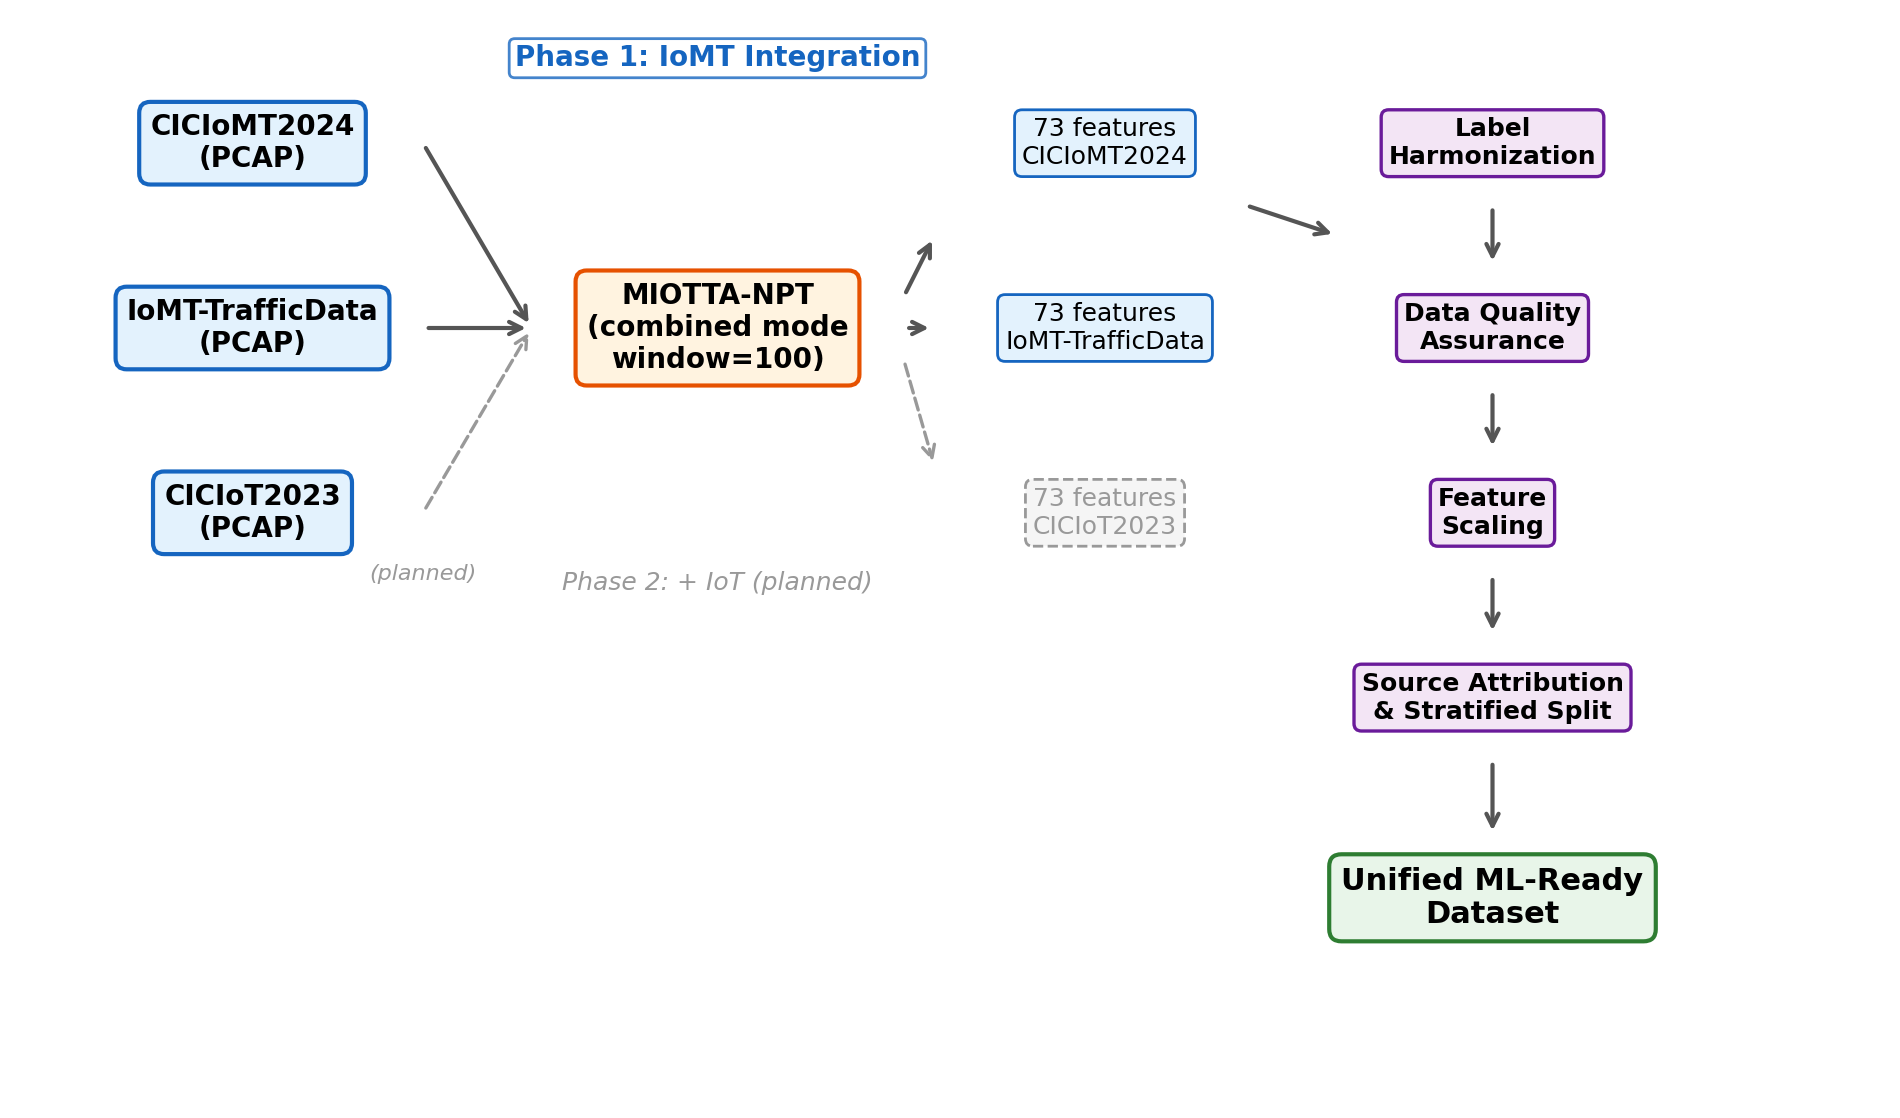
\includegraphics[width=\textwidth]{pipeline_overview.png}
\caption[]{Επισκόπηση της ροής ενοποίησης πολλαπλών σταδίων. Οι ακατέργαστες καταγραφές πακέτων των CICIoMT2024 και IoMT-TrafficData επεξεργάζονται από το MIOTTA-NPT με ταυτόσημη διαμόρφωση και στη συνέχεια περνούν από εναρμόνιση ετικετών, διασφάλιση ποιότητας, κανονικοποίηση και στρωματοποιημένο διαχωρισμό, παράγοντας το τελικό ενοποιημένο σύνολο.}
\label{gr:fig:pipeline}
\end{figure}

\grsubsection{Τυποποιημένη εξαγωγή χαρακτηριστικών}

Όλα τα σύνολα επεξεργάζονται με το MIOTTA-NPT στον συνδυασμένο τρόπο (ροή και παράθυρο) με μέγεθος παραθύρου 100 πακέτων, που εξασφαλίζει ισορροπία μεταξύ χρονικού πλαισίου και υπολογιστικής βιωσιμότητας. Κάθε εγγραφή περιγράφεται από 73 χαρακτηριστικά, οργανωμένα σε ομάδες: μεταδεδομένα σύνδεσης, στατιστικά μεγέθους πακέτων, κατευθυντικές μετρικές, δυναμική ροής, κατανομές σημαιών \gls{tcp}, χρονικά χαρακτηριστικά, δείκτες πρωτοκόλλων και συναθροίσεις επιπέδου παραθύρου.

\grsubsection{Εναρμόνιση ετικετών τριών επιπέδων}

Ορίζεται ιεραρχία ετικετών τριών επιπέδων:
\begin{enumerate}[leftmargin=*, nosep]
  \item \textit{Δυαδικό} (\texttt{label\_binary}): Benign ή Attack.
  \item \textit{Κατηγορίας} (\texttt{label\_category}): έξι λειτουργικές κατηγορίες (Benign, DDoS, DoS, MQTT, Reconnaissance, Spoofing), όπου όλες οι επιθέσεις που σχετίζονται με το \gls{mqtt} ομαδοποιούνται σε ξεχωριστή κατηγορία.
  \item \textit{Λεπτομερές} (\texttt{label\_fine}): οι αρχικές ετικέτες με ομοιόμορφη μορφοποίηση.
\end{enumerate}
Οι αντιστοιχίσεις τηρούνται ως ρητά λεξικά διαμόρφωσης, βασισμένα στις δημοσιεύσεις των συνόλων και σε διαβούλευση με τους επιβλέποντες, ώστε να είναι πλήρως ελέγξιμες.

\grsubsection{Ποιότητα, κανονικοποίηση, προέλευση και διαχωρισμός}

Η διασφάλιση ποιότητας περιλαμβάνει διαχείριση ελλειπουσών τιμών (αφαίρεση χαρακτηριστικών με ποσοστό NaN άνω του 50\% και συμπλήρωση με μηδέν όπου η απουσία οφείλεται σε απουσία πρωτοκόλλου), χειρισμό άπειρων τιμών, αφαίρεση χαρακτηριστικών μηδενικής διασποράς, επισήμανση χαρακτηριστικών σχεδόν μηδενικής διασποράς, αφαίρεση διπλότυπων και ομογενοποίηση τύπων δεδομένων. Η κανονικοποίηση γίνεται με τυποποίηση $z$-score (\texttt{StandardScaler}), της οποίας οι παράμετροι υπολογίζονται \textit{αποκλειστικά} στο σύνολο εκπαίδευσης, ώστε να αποκλείεται η διαρροή πληροφορίας. Κάθε εγγραφή φέρει στήλη προέλευσης (\texttt{source\_dataset}), που επιτρέπει αξιολόγηση μεταξύ πεδίων, ανάλυση ανά πηγή και επικύρωση με εξαίρεση μίας πηγής. Τέλος, ο διαχωρισμός σε εκπαίδευση/επικύρωση/έλεγχο (70/15/15\%) στρωματοποιείται ως προς τον συνδυασμό κατηγορίας και πηγής, ώστε κάθε κατηγορία και κάθε πηγή να εκπροσωπείται αναλογικά σε όλα τα τμήματα.

% ══════════════════════════════════════════════════════════════════════════════
\grsection{Υλοποίηση της ροής ενοποίησης}

\grsubsection{Διερευνητική ανάλυση των αρχικών συνόλων}

Το αρχικό CICIoMT2024 περιλαμβάνει 8.322.896 εγγραφές με 45 αριθμητικά χαρακτηριστικά, 18 τύπους επιθέσεων σε πέντε κατηγορίες και έντονη ανισορροπία κλάσεων (λόγος μέγιστης προς ελάχιστη κλάση $\approx$ 2.157:1)· η κίνηση επιθέσεων αντιστοιχεί στο 98,4\% των εγγραφών. Το IoMT-TrafficData περιλαμβάνει 969.141 εγγραφές ροών με 101 χαρακτηριστικά του Zeek και οκτώ τύπους επιθέσεων (ARP Spoofing, Apache Killer, CAM Table Overflow, MQTT Malaria, Netscan, RUDY, Slow Loris, Slow Read). Η θεμελιώδης δομική ασυμβατότητα των δύο σχημάτων (παράθυρα DPKT έναντι ροών Zeek, 45 έναντι 101 χαρακτηριστικών με διαφορετική σημασιολογία) επιβεβαίωσε ότι η σημασιολογική αντιστοίχιση δεν επαρκεί και ότι απαιτείται επανεξαγωγή από τα \gls{pcap}.

\grsubsection{Επεξεργασία με MIOTTA-NPT και επαλήθευση}

Η επεξεργασία με MIOTTA-NPT παρήγαγε 8.423.955 εγγραφές για το CICIoMT2024 (και οι 18 τύποι επιθέσεων και η καλόβουλη κίνηση) και 184.241 εγγραφές για το IoMT-TrafficData. Η εμπειρική σύγκριση επιβεβαίωσε ότι τα δύο σύνολα έχουν ακριβώς τις ίδιες 73 στήλες, με ίδια ονόματα και τύπους, χωρίς αποκλειστικές στήλες. Οι κατανομές τιμών διαφέρουν μεταξύ των πηγών, γεγονός αναμενόμενο και επιθυμητό, καθώς αποτυπώνει την πραγματική ποικιλομορφία των περιβαλλόντων. Οι ελλείπουσες τιμές συγκεντρώνονται στις σημαίες \gls{tcp} και οφείλονται σε παράθυρα που περιέχουν αποκλειστικά κίνηση άλλων πρωτοκόλλων.

\grsubsection{Εναρμόνιση ετικετών και διασφάλιση ποιότητας}

Οι 19 αρχικές ετικέτες του CICIoMT2024 και οι 10 του IoMT-TrafficData αντιστοιχίστηκαν πλήρως στο σχήμα τριών επιπέδων, χωρίς καμία μη αντιστοιχισμένη ετικέτα. Μετά τη συνένωση (8.608.196 εγγραφές, 73 χαρακτηριστικά), η διασφάλιση ποιότητας εκτελέστηκε σε έξι βήματα: αφαιρέθηκαν οκτώ χαρακτηριστικά σημαιών \gls{tcp} με 98,28\% ελλείπουσες τιμές· δεν εντοπίστηκε καμία άπειρη τιμή· αφαιρέθηκαν επτά χαρακτηριστικά μηδενικής διασποράς· επισημάνθηκαν (χωρίς αφαίρεση) τέσσερα χαρακτηριστικά σχεδόν μηδενικής διασποράς· αφαιρέθηκαν 596.662 διπλότυπες εγγραφές (6,93\%), που οφείλονται κυρίως σε επαναλαμβανόμενα παράθυρα επιθέσεων πλημμύρας· και όλα τα χαρακτηριστικά μετατράπηκαν σε \texttt{float32}. Το τελικό σύνολο περιλαμβάνει \textbf{8.011.534 εγγραφές} και \textbf{58 χαρακτηριστικά}.

\grsubsection{Το τελικό ενοποιημένο σύνολο δεδομένων}

Ο στρωματοποιημένος διαχωρισμός απέδωσε τρία τμήματα: 5.608.073 εγγραφές εκπαίδευσης, 1.201.730 επικύρωσης και 1.201.731 ελέγχου, με σχεδόν ταυτόσημες αναλογίες κατηγοριών και πηγών σε κάθε τμήμα (απόκλιση πηγών εντός $\pm$0,01\%). Ο Πίνακας~\ref{gr:tab:classes} παρουσιάζει την κατανομή των κατηγοριών ανά πηγή. Το σύνολο κυριαρχείται από επιθέσεις (99,33\%), με λόγο μέγιστης προς ελάχιστη κατηγορία περίπου 575:1 (DDoS έναντι Spoofing). Οι δύο πηγές είναι συμπληρωματικές: το CICIoMT2024 συνεισφέρει το 97,70\% των εγγραφών και όλη την κίνηση DDoS, ενώ το IoMT-TrafficData εισάγει έξι λεπτομερείς τύπους επιθέσεων που δεν υπάρχουν στο CICIoMT2024 (Apache\_Killer, CAM\_Table\_Overflow, MQTT\_Malaria, RUDY, SlowLoris, SlowRead). Συνολικά υπάρχουν 26 λεπτομερείς ετικέτες, ενώ οι ετικέτες Benign και ARP\_Spoofing εμφανίζονται και στις δύο πηγές, επιτρέποντας άμεση σύγκριση μεταξύ περιβαλλόντων. Το σύνολο δημοσιεύθηκε στο αποθετήριο CORA (Dataverse)~\cite{unified_iomt_csuc2026} μαζί με τον προσαρμοσμένο κανονικοποιητή (\texttt{scaler.joblib}) και τα μεταδεδομένα της ροής.

\begin{table}[!htbp]
\centering
\caption[]{Κατανομή των κατηγοριών (επίπεδο 2) ανά πηγή στο τελικό ενοποιημένο σύνολο δεδομένων.}
\label{gr:tab:classes}
\small
\begin{tabular}{@{}l r r r r@{}}
\toprule
\textbf{Κατηγορία} & \textbf{CICIoMT2024} & \textbf{IoMT-TrafficData} & \textbf{Σύνολο} & \textbf{Ποσοστό} \\
\midrule
DDoS           & 5.368.292 & 0      & 5.368.292 & 67,01\% \\
DoS            & 2.100.735 & 47.742 & 2.148.477 & 26,82\% \\
MQTT           & 320.204   & 65.734 & 385.938   & 4,82\% \\
Benign         & 23.133    & 30.323 & 53.456    & 0,67\% \\
Reconnaissance & 13.147    & 32.879 & 46.026    & 0,57\% \\
Spoofing       & 1.782     & 7.563  & 9.345     & 0,12\% \\
\midrule
\textbf{Σύνολο} & \textbf{7.827.293} & \textbf{184.241} & \textbf{8.011.534} & \textbf{100\%} \\
\bottomrule
\end{tabular}
\end{table}

% ══════════════════════════════════════════════════════════════════════════════
\grsection{Πειραματική αξιολόγηση}

\grsubsection{Αξιολόγηση ποιότητας του ενοποιημένου συνόλου}

Ο έλεγχος δομικής ακεραιότητας επιβεβαίωσε μηδενικές ελλείπουσες και άπειρες τιμές, συνέπεια τύπων, απουσία σταθερών χαρακτηριστικών, πλήρως συμπληρωμένες στήλες ετικετών και προέλευσης, καθώς και τμήματα διαχωρισμού χωρίς επικάλυψη. Στο σύνολο εκπαίδευσης οι μέσοι όροι των χαρακτηριστικών είναι πρακτικά μηδενικοί και οι τυπικές αποκλίσεις ίσες με 1, ενώ στα σύνολα επικύρωσης και ελέγχου οι μικρές αποκλίσεις (μέγιστη απόλυτη μέση τιμή 0,0013 και 0,0026) επιβεβαιώνουν την απουσία διαρροής. Τα περισσότερα χαρακτηριστικά παρουσιάζουν βαριές ουρές (52 από τα 58 με $|\text{ασυμμετρία}| > 2$), χαρακτηριστικό της δικτυακής κίνησης. Η προβολή PCA έδειξε μερική επικάλυψη των πηγών στον μειωμένο χώρο, γεγονός που υποστηρίζει την ενιαία μάθηση, ενώ διατηρούνται οι γνήσιες διαφορές μεταξύ των περιβαλλόντων.

\grsubsection{Πειραματικό πλαίσιο}

Αξιολογήθηκαν τρεις ταξινομητές αυξανόμενης πολυπλοκότητας: Δέντρο Απόφασης (DT), Τυχαίο Δάσος (RF) και XGBoost, καθώς τα μοντέλα βασισμένα σε δέντρα ανταγωνίζονται ή υπερτερούν της βαθιάς μάθησης σε πινακοειδή δεδομένα~\cite{grinsztajn2022tree}. Οι έξι κατηγορίες κωδικοποιούνται με κοινή (καθολική) αντιστοίχιση, ώστε οι πίνακες σύγχυσης να είναι συγκρίσιμοι μεταξύ πειραμάτων. Η ανισορροπία αντιμετωπίζεται με ισορροπημένα βάρη κλάσεων (DT, RF) ή ισοδύναμα βάρη δειγμάτων (XGBoost), χωρίς συνθετική υπερδειγματοληψία. Για να απομονωθεί η επίδραση της ενοποίησης, ορίστηκαν τρία καθεστώτα εκπαίδευσης που διαφέρουν \textit{μόνο} ως προς τις εγγραφές εκπαίδευσης: \textbf{B1} (μόνο CICIoMT2024), \textbf{B2} (μόνο IoMT-TrafficData) και \textbf{U} (ενοποιημένο). Οι υπερπαράμετροι ρυθμίστηκαν με \texttt{RandomizedSearchCV} (50 επαναλήψεις, στρωματοποιημένη διασταυρωμένη επικύρωση 3 τμημάτων, κριτήριο macro-F1)· για RF και XGBoost η αναζήτηση έγινε σε στρωματοποιημένο υποδείγμα 300.000 εγγραφών και το τελικό μοντέλο εκπαιδεύτηκε σε ολόκληρο το σύνολο εκπαίδευσης. Σύμφωνα με τις συστάσεις του Lones~\cite{lones2024avoid}, το σύνολο ελέγχου χρησιμοποιήθηκε μία μόνο φορά ανά μοντέλο. Κάθε μοντέλο αξιολογείται σε τρία τμήματα ελέγχου: εντός πεδίου, στο άλλο πεδίο (cross-domain) και στο πλήρες σύνολο ελέγχου. Κύρια μετρική είναι το macro-F1, που αποδίδει ίσο βάρος σε κάθε κλάση· η ακρίβεια (accuracy) αναφέρεται μόνο συμπληρωματικά λόγω της ανισορροπίας.

\grsubsection{Κατάρρευση των μοντέλων μίας πηγής και ενοποιημένη εκπαίδευση}

Ο Πίνακας~\ref{gr:tab:regimes} συγκεντρώνει τα αποτελέσματα των ρυθμισμένων μοντέλων. Τα μοντέλα μίας πηγής αποδίδουν ικανοποιητικά εντός πεδίου, αλλά καταρρέουν στο άλλο πεδίο: έως 0,0523 για B2$\to$CIC με DT και το πολύ 0,3423 για B1$\to$IoMT με RF. Η ασυμμετρία εξηγείται δομικά: ένα μοντέλο B2 δεν έχει δει ποτέ κίνηση DDoS, η οποία αποτελεί την κυρίαρχη κλάση του τμήματος CIC. Αντίθετα, τα μοντέλα του καθεστώτος U επιτυγχάνουν macro-F1 $\geq 0{,}926$ στο τμήμα CIC, $\geq 0{,}999$ στο τμήμα IoMT (επί των πέντε παρουσών κλάσεων) και $\geq 0{,}948$ στο πλήρες σύνολο ελέγχου.

\begin{table}[!htbp]
\centering
\caption[]{Macro-F1 των ρυθμισμένων μοντέλων ανά καθεστώς εκπαίδευσης και τμήμα ελέγχου. Με «(εντός)» σημειώνεται το τμήμα της ίδιας πηγής και με «(άλλο)» το τμήμα της άλλης πηγής.}
\label{gr:tab:regimes}
\small
\begin{tabular}{@{}l l c c c@{}}
\toprule
\textbf{Καθεστώς} & \textbf{Μοντέλο} & \textbf{Τμήμα CIC} & \textbf{Τμήμα IoMT} & \textbf{Πλήρες σύνολο} \\
\midrule
\multirow{3}{*}{B1 (μόνο CIC)}  & DT  & 0,9226 (εντός) & 0,2474 (άλλο) & 0,6959 \\
                                & RF  & 0,9149 (εντός) & 0,3423 (άλλο) & 0,7395 \\
                                & XGB & 0,9410 (εντός) & 0,2724 (άλλο) & 0,7199 \\
\midrule
\multirow{3}{*}{B2 (μόνο IoMT)} & DT  & 0,0523 (άλλο) & 0,8332 (εντός) & 0,3284 \\
                                & RF  & 0,0586 (άλλο) & 0,8333 (εντός) & 0,2029 \\
                                & XGB & 0,1079 (άλλο) & 0,8333 (εντός) & 0,3708 \\
\midrule
\multirow{3}{*}{U (ενοποιημένο)} & DT  & 0,9262 & 0,9990\textsuperscript{*} & 0,9480 \\
                                 & RF  & 0,9285 & 0,9995\textsuperscript{*} & 0,9487 \\
                                 & XGB & 0,9382 & 0,9999\textsuperscript{*} & \textbf{0,9522} \\
\bottomrule
\end{tabular}

\vspace{0.3em}
\raggedright\footnotesize
\textsuperscript{*}\,Υπολογισμένο επί των πέντε κλάσεων που υπάρχουν στο τμήμα IoMT (δεν περιέχει DDoS)· το macro-F1 επί και των έξι κλάσεων είναι $\approx$ 0,833.
\end{table}

Η μετάβαση από το καλύτερο μοντέλο μίας πηγής στο πλήρες σύνολο ελέγχου (RF-B1, 0,7395) στο ασθενέστερο ενοποιημένο μοντέλο (DT-U, 0,9480) αντιστοιχεί σε βελτίωση $+20{,}85$ ποσοστιαίων μονάδων, ενώ η διαφορά μεταξύ των τριών ενοποιημένων μοντέλων είναι μόλις 0,42 μονάδες. Η συνεισφορά της ενοποίησης είναι επομένως περίπου \textbf{50 φορές μεγαλύτερη} από τη συνεισφορά της πολυπλοκότητας του μοντέλου.

\grsubsection{Ανάλυση ανά κλάση}

Στο καλύτερο μοντέλο (XGBoost-U), τέσσερις από τις έξι κατηγορίες (Benign, MQTT, Reconnaissance, Spoofing) ταξινομούνται με F1 $\geq 0{,}98$· η κατηγορία Spoofing επιτυγχάνει F1 = 0,98 παρότι αντιστοιχεί μόλις στο 0,12\% των δεδομένων, χάρη στα ισορροπημένα βάρη και στο διακριτό αποτύπωμα του ARP Spoofing. Όπως φαίνεται στο Σχήμα~\ref{gr:fig:cm}, το κυρίαρχο υπολειπόμενο σφάλμα είναι η αμφίδρομη σύγχυση DDoS$\leftrightarrow$DoS, η οποία ευθύνεται για περισσότερο από το 99\% των σφαλμάτων και στα τρία μοντέλα. Η σύγχυση αυτή είναι αναμενόμενη: οι επιθέσεις DDoS και DoS τύπου TCP/IP (πλημμύρες SYN, ICMP, UDP, TCP) έχουν σχεδόν ταυτόσημα στατιστικά ανά παράθυρο, ενώ ο διακριτικός παράγοντας, δηλαδή το πλήθος των πηγών επίθεσης, δεν αποτυπώνεται στα 58 χαρακτηριστικά. Το γεγονός ότι το F1 της κλάσης DoS παραμένει 0,82 και στα τρία μοντέλα, ενώ της DDoS αυξάνεται οριακά από 0,91 σε 0,92, υποδεικνύει περιορισμό της \textit{αναπαράστασης χαρακτηριστικών} και όχι της \textit{χωρητικότητας του μοντέλου}.

\begin{figure}[!htbp]
\centering
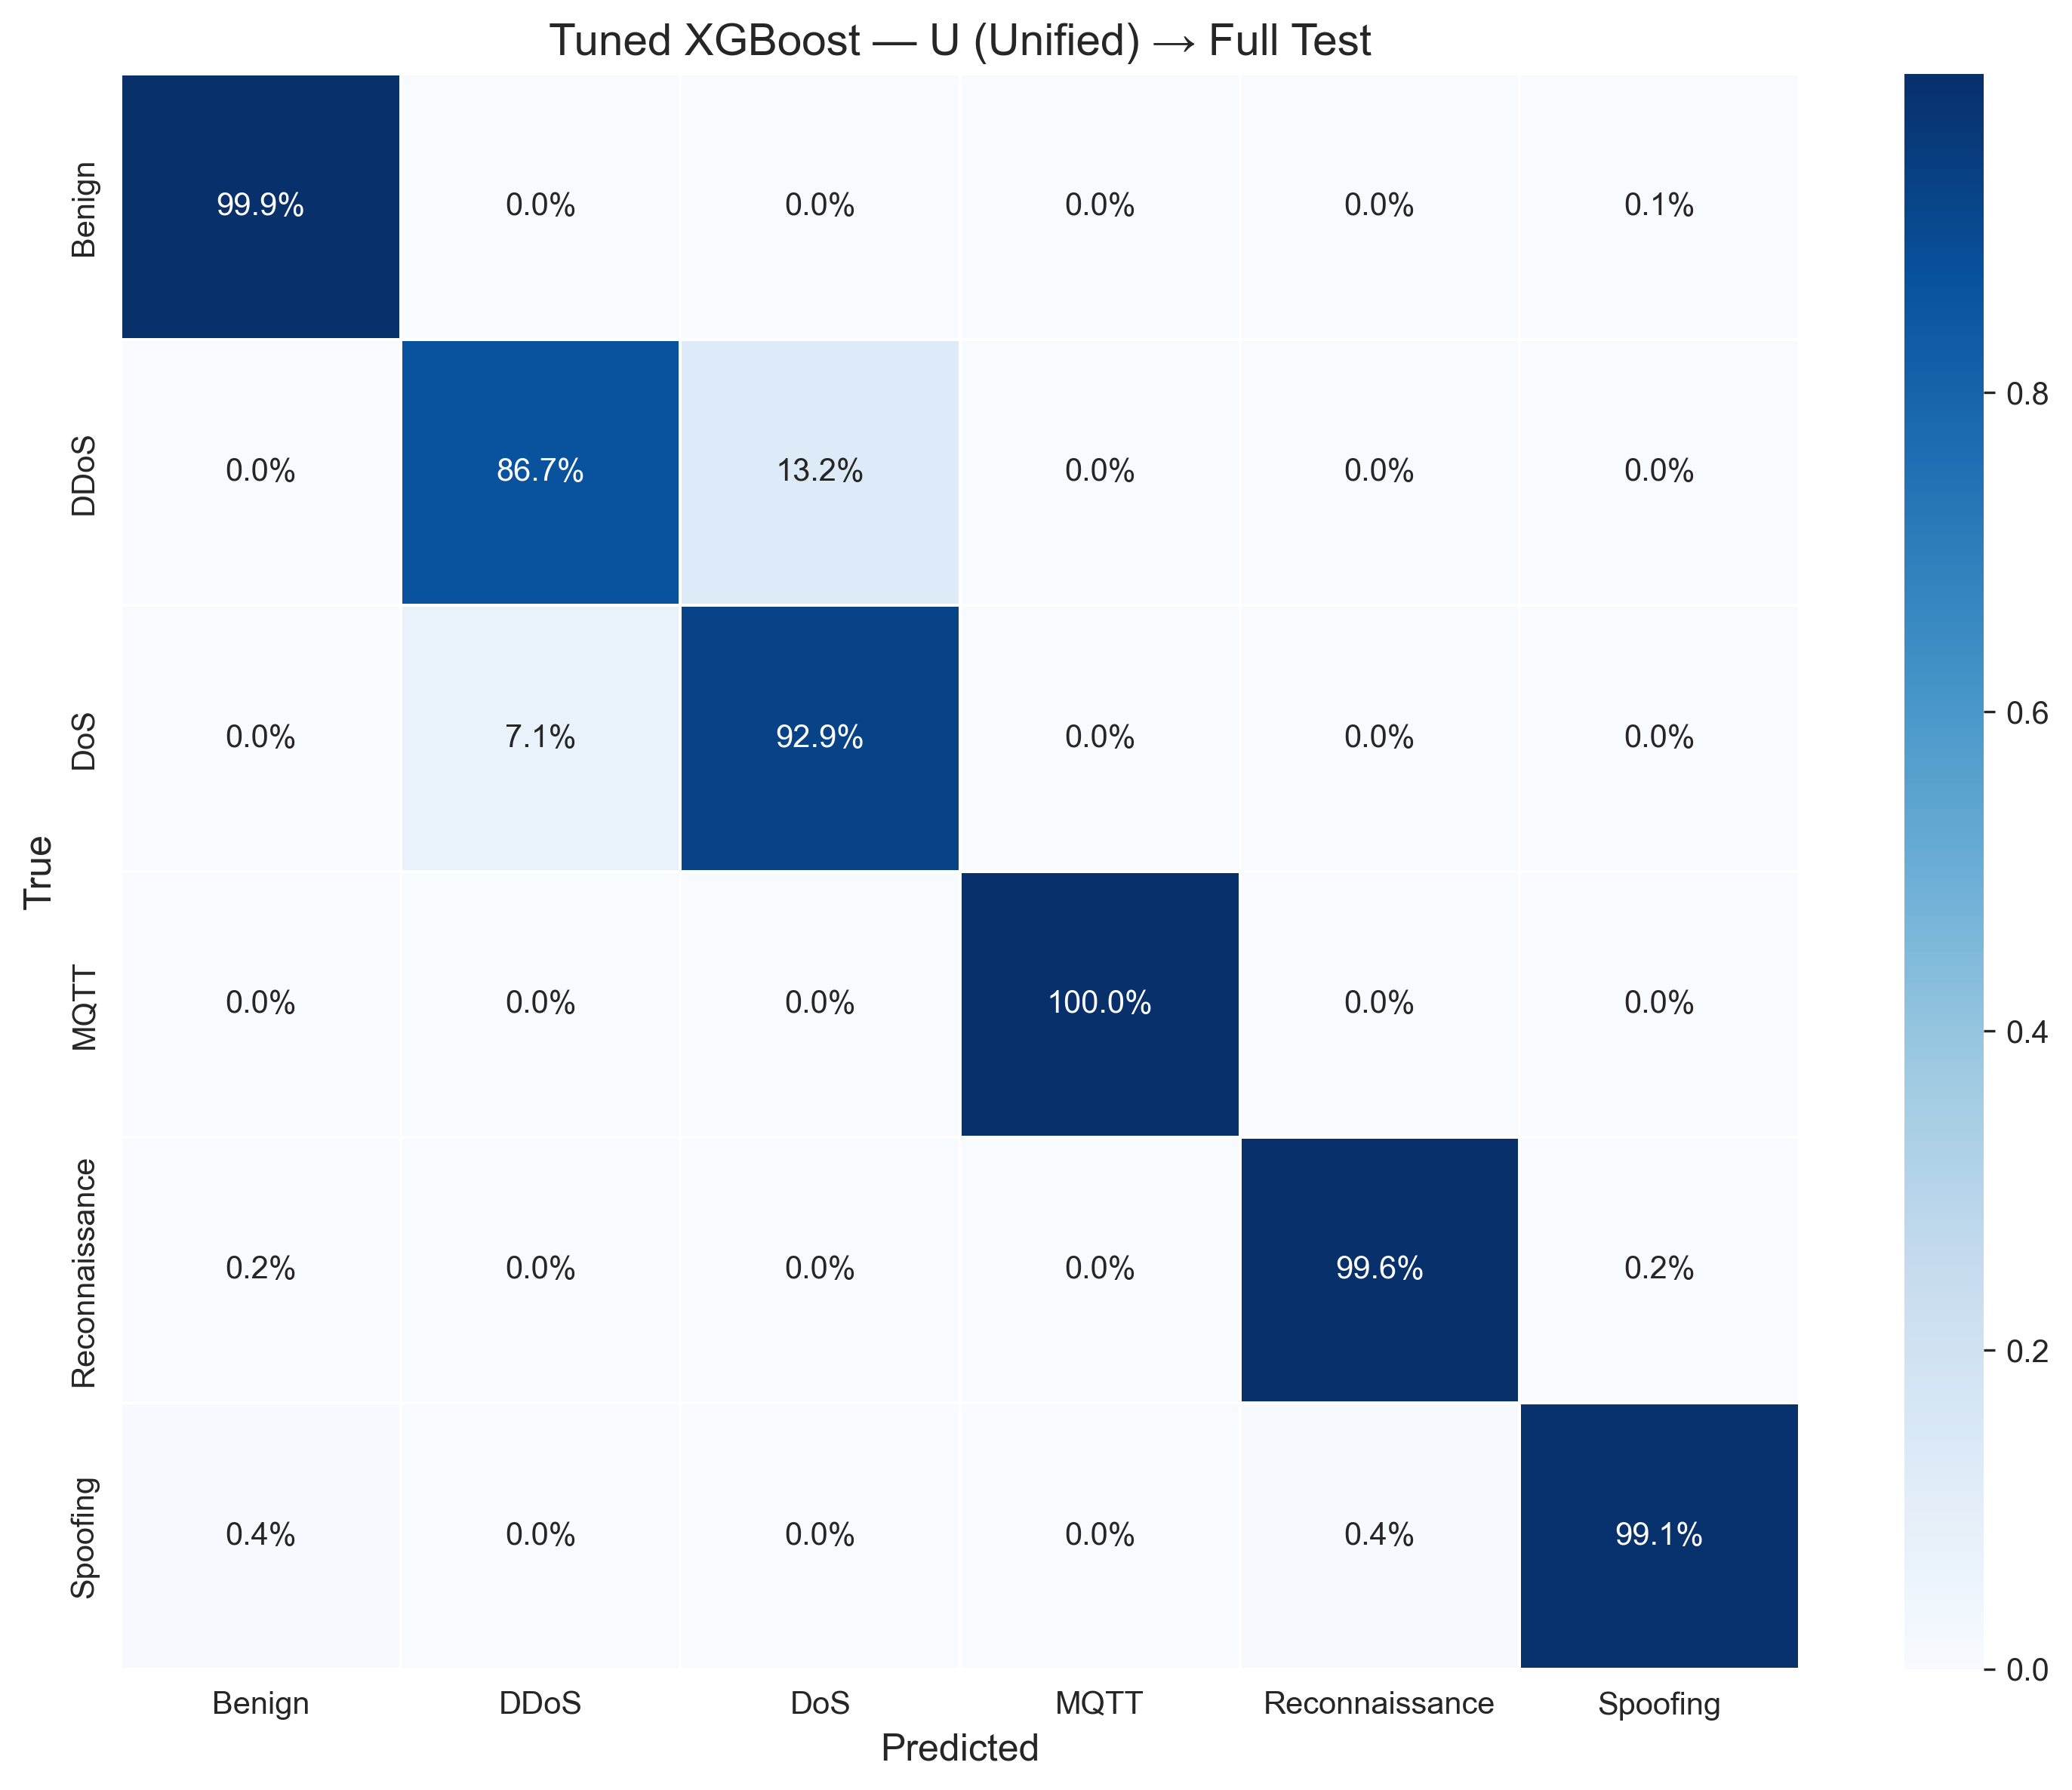
\includegraphics[width=0.62\textwidth]{ch5_xgb_cm_u_full.png}
\caption[]{Κανονικοποιημένος πίνακας σύγχυσης του ρυθμισμένου μοντέλου XGBoost (ενοποιημένο καθεστώς) στο πλήρες σύνολο ελέγχου (1.201.731 δείγματα). Τα σφάλματα συγκεντρώνονται σχεδόν αποκλειστικά στο ζεύγος DDoS--DoS.}
\label{gr:fig:cm}
\end{figure}

Το Σχήμα~\ref{gr:fig:perclass} συγκρίνει το F1 ανά κλάση για τα τρία καθεστώτα του XGBoost: η εκπαίδευση μίας πηγής καταρρέει στις κλάσεις της άλλης πηγής, ενώ το ενοποιημένο μοντέλο ανακτά και τις έξι κλάσεις.

\begin{figure}[!htbp]
\centering
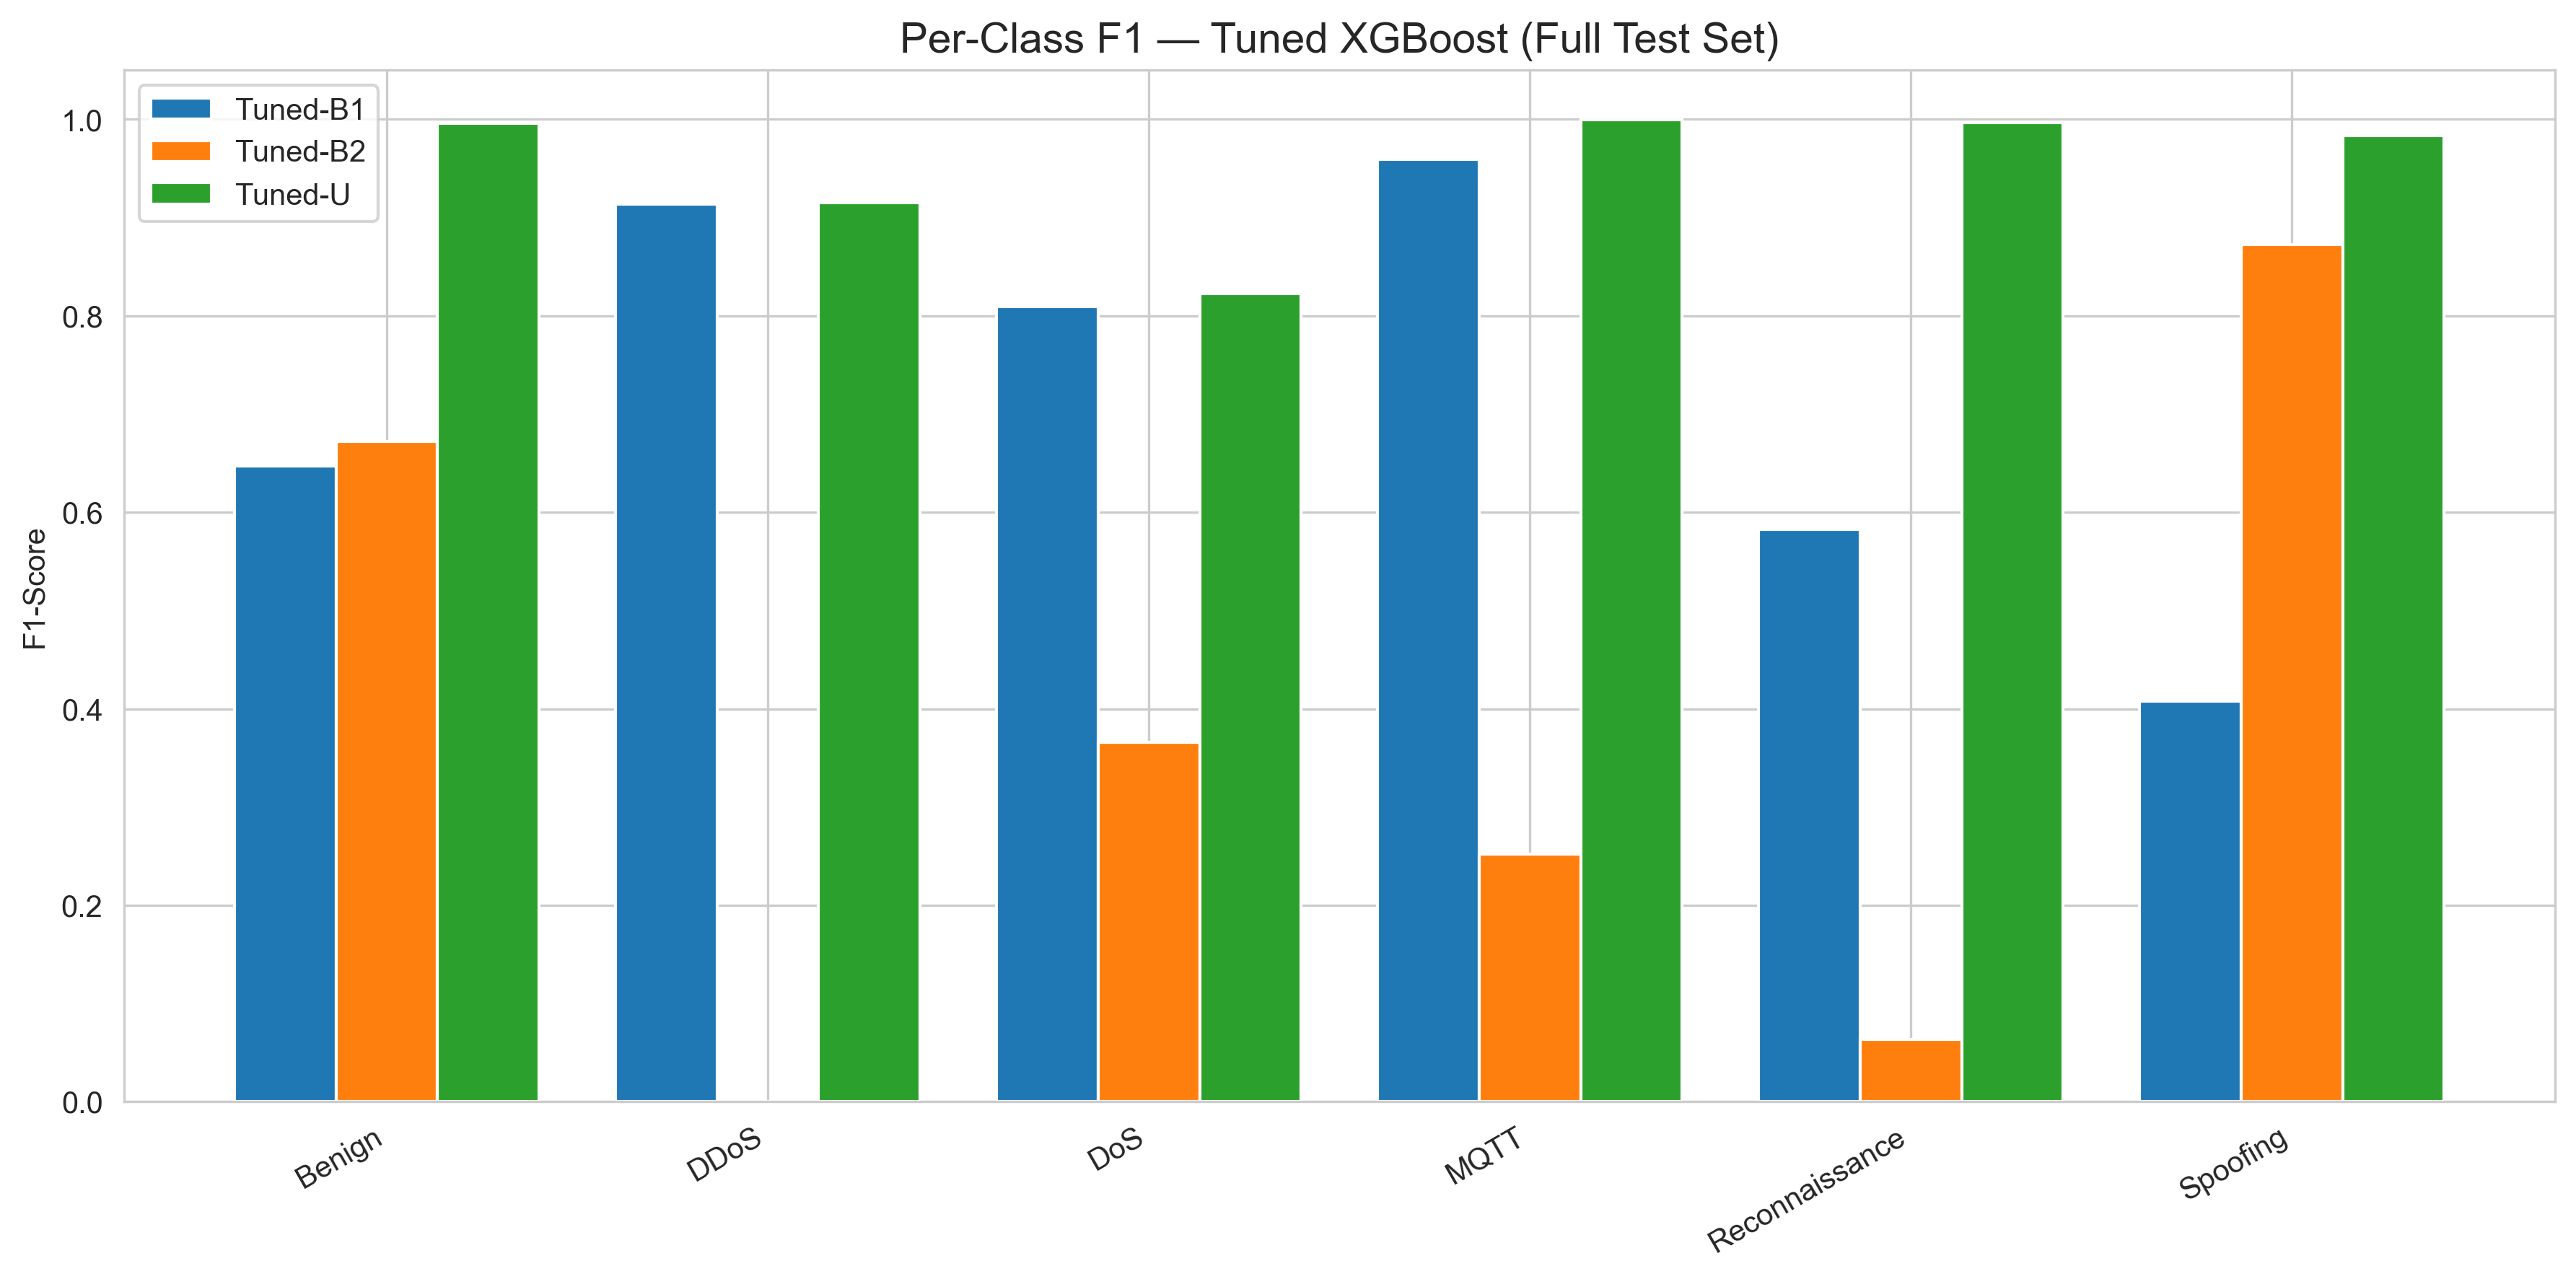
\includegraphics[width=\textwidth]{ch5_xgb_per_class_f1.png}
\caption[]{Σύγκριση του F1 ανά κλάση μεταξύ των καθεστώτων εκπαίδευσης B1, B2 και U (ρυθμισμένο XGBoost, πλήρες σύνολο ελέγχου).}
\label{gr:fig:perclass}
\end{figure}

\grsubsection{Στατιστική σημαντικότητα}

Η σημαντικότητα των διαφορών μεταξύ των ενοποιημένων μοντέλων ελέγχθηκε με τον έλεγχο McNemar~\cite{mcnemar1947note} με διόρθωση συνέχειας Yates, κατάλληλο για ζευγαρωτές παρατηρήσεις στο ίδιο σύνολο ελέγχου. Επειδή με $N = 1.201.731$ δείγματα ακόμη και αμελητέες διαφορές γίνονται στατιστικά σημαντικές, αναφέρεται επιπλέον η σχετική μείωση σφάλματος (RER) ως μέτρο μεγέθους επίδρασης (Πίνακας~\ref{gr:tab:mcnemar}). Το XGBoost υπερέχει στατιστικά και πρακτικά έναντι των DT και RF (RER $\approx$ 3\%, δηλαδή περίπου 4.000 λιγότερα σφάλματα). Η σύγκριση DT--RF είναι στατιστικά σημαντική αλλά πρακτικά οριακή: το RF κάνει ελαφρώς περισσότερα συνολικά σφάλματα, έχει όμως υψηλότερο macro-F1, επειδή μεταφέρει σφάλματα από τις μειοψηφικές κλάσεις προς το όριο DDoS/DoS, που είναι και η επιδιωκόμενη συμπεριφορά της εκπαίδευσης με ισορροπημένα βάρη.

\begin{table}[!htbp]
\centering
\caption[]{Έλεγχος McNemar για τις ζευγαρωτές συγκρίσεις των ενοποιημένων μοντέλων στο πλήρες σύνολο ελέγχου. $b$: το Α σωστό και το Β λάθος· $c$: το Α λάθος και το Β σωστό· RER $> 0$: το Β κάνει λιγότερα σφάλματα.}
\label{gr:tab:mcnemar}
\small
\begin{tabular}{@{}l c c r r r@{}}
\toprule
\textbf{Ζεύγος (Α έναντι Β)} & $b$ & $c$ & $\chi^2$ (Yates) & \textbf{τιμή $p$} & \textbf{RER (\%)} \\
\midrule
DT έναντι RF  & 6.919 & 6.372  & 22,43    & $2{,}2 \times 10^{-6}$ & $-0{,}41$ \\
DT έναντι XGB & 7.314 & 11.297 & 851,99   & $< 10^{-15}$ & $+2{,}98$ \\
RF έναντι XGB & 4.246 & 8.776  & 1.575,17 & $< 10^{-15}$ & $+3{,}38$ \\
\bottomrule
\end{tabular}
\end{table}

% ══════════════════════════════════════════════════════════════════════════════
\grsection{Γενίκευση σε πραγματική νοσοκομειακή κίνηση: HospNet26}

\grsubsection{Σύνολο δεδομένων και πρωτόκολλο}

Το HospNet26~\cite{hospnet26} είναι δημόσιο σύνολο αναφοράς με ανωνυμοποιημένα χαρακτηριστικά κίνησης από το εσωτερικό δίκτυο ενός νοσοκομείου Helios στη Γερμανία, που καταγράφηκε κατά τη διάρκεια μίας εβδομάδας κανονικής κλινικής λειτουργίας (Αύγουστος 2025). Δεν περιέχει ετικέτες επιθέσεων: τεκμηριώνεται ως αποκλειστικά νόμιμη κίνηση και κάθε πρόβλεψη διαφορετική από Benign αποτελεί ψευδώς θετικό. Τα τέσσερα χρονικά τμήματα (Παρασκευή, Σαββατοκύριακο, Δευτέρα, Δευτέρα--Παρασκευή) συνενώθηκαν σε \textbf{1.265.240 παράθυρα}· εξήχθησαν τα 58 χαρακτηριστικά με την ίδια σειρά, εφαρμόστηκε ο \textit{ίδιος} κανονικοποιητής του συνόλου εκπαίδευσης (χωρίς νέα προσαρμογή) και τα τρία ενοποιημένα μοντέλα εφαρμόστηκαν χωρίς επανεκπαίδευση. Ως μετρική χρησιμοποιείται το ποσοστό προβλέψεων Benign $r_B$, το οποίο στη συγκεκριμένη περίπτωση ισούται με την ειδικότητα του μοντέλου.

\grsubsection{Αποτελέσματα}

Όπως δείχνει ο Πίνακας~\ref{gr:tab:hospnet}, και τα τρία μοντέλα ταξινομούν το 90--96\% της πραγματικής νοσοκομειακής κίνησης ως κάποια μορφή επίθεσης, με $r_B$ μόλις 3,72--9,96\%. Η κυρίαρχη κλάση ψευδώς θετικών είναι η DoS (51--72\% των παραθύρων). Το XGBoost επιτυγχάνει το υψηλότερο $r_B$ (9,96\%). Τα παράθυρα του Σαββατοκύριακου εμφανίζουν ακόμη χαμηλότερα ποσοστά Benign (0,86--5,86\%) από τις καθημερινές, γεγονός που υποδηλώνει χρονικά μη στάσιμη μετατόπιση κατανομής. Συμπληρωματικά, στο σχετικό άρθρο δείχνεται ότι και τα μοντέλα μίας πηγής (B1, B2) παραμένουν στην ίδια ζώνη 0--10\%· άρα το χάσμα δεν κλείνει με αλλαγή της σύνθεσης των εργαστηριακών δεδομένων εκπαίδευσης.

\begin{table}[!htbp]
\centering
\caption[]{Κατανομή προβλέψεων των τριών ρυθμισμένων ενοποιημένων μοντέλων σε 1.265.240 παράθυρα πραγματικής νοσοκομειακής κίνησης (HospNet26). Όλη η κίνηση είναι καλόβουλη, επομένως η τελευταία στήλη ($r_B$) είναι η ειδικότητα του μοντέλου και όλες οι υπόλοιπες στήλες είναι ποσοστά ψευδώς θετικών.}
\label{gr:tab:hospnet}
\small
\begin{tabular}{@{}l r r r r r r | r@{}}
\toprule
\textbf{Μοντέλο} & \textbf{Benign} & \textbf{DDoS} & \textbf{DoS} & \textbf{MQTT} & \textbf{Recon.} & \textbf{Spoofing} & \textbf{$r_B$} \\
\midrule
Decision Tree  & 6,07\% &  7,80\% & 72,04\% & 0,22\% &  5,30\% &  8,57\% & \textbf{6,07\%} \\
Random Forest  & 3,72\% &  0,60\% & 71,37\% & 0,06\% & 19,08\% &  5,17\% & \textbf{3,72\%} \\
XGBoost        & 9,96\% & 23,80\% & 51,14\% & 0,11\% &  4,28\% & 10,71\% & \textbf{9,96\%} \\
\bottomrule
\end{tabular}
\end{table}

\grsubsection{Ερμηνεία και στρατηγικές επαναβαθμονόμησης}

Το αποτέλεσμα δεν αποτελεί αποτυχία του μοντέλου, αλλά περίπτωση \textit{μετατόπισης συμμεταβλητών} (covariate shift)~\cite{sommer2010outside}: η κατανομή των καλόβουλων δεδομένων εκπαίδευσης διαφέρει συστηματικά από εκείνη του περιβάλλοντος λειτουργίας. Η καλόβουλη κίνηση των εργαστηριακών συνόλων παρήχθη υπό ελεγχόμενες συνθήκες, ενώ ένα πραγματικό νοσοκομείο μεταφέρει ροές ιατρικής απεικόνισης (DICOM/PACS), συστήματα ηλεκτρονικού φακέλου υγείας (HL7, FHIR), ιδιόκτητα κλινικά πρωτόκολλα και μεγάλο όγκο διοικητικής κίνησης. Οι μεταφορές υψηλού ρυθμού παράγουν στατιστικά τύπου «ριπής» που επικαλύπτονται με την περιοχή χαρακτηριστικών της κλάσης DoS, κάτι που εξηγεί γιατί η DoS κυριαρχεί στα ψευδώς θετικά. Για τη γεφύρωση του χάσματος προτείνονται δύο στρατηγικές χαμηλού κόστους: (α)~\textit{λεπτομερής προσαρμογή με λίγα δείγματα} (few-shot fine-tuning), δηλαδή επανεκπαίδευση με ένα μικρό, επιβεβαιωμένα καλόβουλο δείγμα από το νοσοκομείο-στόχο (περίπου 10.000--50.000 παράθυρα)· και (β)~\textit{εκ των υστέρων βαθμονόμηση κατωφλίου} στις πιθανότητες εξόδου του μοντέλου, με στόχο αποδεκτό ποσοστό ψευδών συναγερμών (π.χ.\ $\leq 1\%$). Και οι δύο απαιτούν μόνο καλόβουλη κίνηση, που είναι άφθονη σε κάθε δίκτυο, και αποφεύγουν τα ηθικά και πρακτικά προβλήματα συλλογής επισημασμένων επιθέσεων σε πραγματικό νοσοκομείο.

% ══════════════════════════════════════════════════════════════════════════════
\grsection{Βιωσιμότητα και ηθικές διαστάσεις}

Από περιβαλλοντική σκοπιά, η εργασία εκτελέστηκε σε συμβατικό υλικό, χωρίς συστοιχίες υψηλών επιδόσεων· η προτίμηση αποδοτικών αλγορίθμων με δέντρα και η δημοσίευση ενός επαναχρησιμοποιήσιμου συνόλου μειώνουν τον υπολογιστικό φόρτο που θα απαιτούσε η επανάληψη της ίδιας προεπεξεργασίας από κάθε ερευνητή. Από οικονομική σκοπιά, όλα τα εργαλεία και τα σύνολα δεδομένων είναι ανοικτά, με ελάχιστο άμεσο κόστος, ενώ το δημόσιο σύνολο (DOI \texttt{10.34810/DATA3305}) αυξάνει τη μακροπρόθεσμη αξία της εργασίας. Κοινωνικά, η εργασία συμβάλλει στην προστασία κρίσιμων υποδομών υγείας και στη διάχυση της γνώσης μέσω αναπαραγώγιμης μεθοδολογίας. Από ηθική σκοπιά, τα σύνολα εκπαίδευσης προέρχονται από ελεγχόμενες πειραματικές διατάξεις χωρίς δεδομένα ασθενών, τα στατιστικά χαρακτηριστικά δεν διατηρούν αναγνωριστικά δικτύου, η εργασία έχει αμιγώς αμυντικό προσανατολισμό και η καταγραφή προέλευσης επιτρέπει τον εντοπισμό μεροληψιών ανά πηγή.

% ══════════════════════════════════════════════════════════════════════════════
\grsection{Συμπεράσματα}

\grsubsection{Απάντηση στο ερευνητικό ερώτημα}

Η απάντηση στο ερευνητικό ερώτημα έχει τρία σκέλη. \textit{Πώς επιτυγχάνεται η ενοποίηση:} με εφαρμογή ενός κοινού εργαλείου εξαγωγής χαρακτηριστικών (MIOTTA-NPT) στις ακατέργαστες καταγραφές κάθε πηγής, εναρμόνιση των ετικετών σε κοινή ταξινομία και συνένωση των εγγραφών με μεταδεδομένα προέλευσης· έτσι αίρονται τα δομικά εμπόδια (Π2, Π3) που αποκλείουν την απλή συνένωση. \textit{Αν βελτιώνει την απόδοση:} ναι· η ενοποιημένη εκπαίδευση αύξησε το macro-F1 στο ετερογενές σύνολο ελέγχου από 0,70--0,74 (καλύτερο μοντέλο μίας πηγής) σε 0,948--0,952, με υψηλή απόδοση και στις έξι κατηγορίες. \textit{Ποια είναι τα όριά της:} η ενοποίηση εργαστηριακών πηγών βελτιώνει τη γενίκευση \textit{μεταξύ αυτών των πηγών}, αλλά δεν κλείνει το χάσμα προς τα πραγματικά κλινικά περιβάλλοντα· η γενίκευση σε επίπεδο λειτουργίας απαιτεί αντιπροσωπευτικά δείγματα από το δίκτυο-στόχο, όπως έδειξε η αξιολόγηση στο HospNet26.

\grsubsection{Περιορισμοί}

Τα ευρήματα πρέπει να ερμηνεύονται λαμβάνοντας υπόψη ότι: (i)~τα δεδομένα εκπαίδευσης προέρχονται από εργαστηριακές διατάξεις· (ii)~ενοποιήθηκαν μόνο δύο πηγές· (iii)~το μέγεθος παραθύρου (100 πακέτα) διατηρήθηκε σταθερό· (iv)~η εναρμόνιση ετικετών περιλαμβάνει υποκειμενικές επιλογές· (v)~το HospNet26 δεν διαθέτει επισημασμένη αλήθεια εδάφους, οπότε κάποια «ψευδώς θετικά» θα μπορούσαν θεωρητικά να είναι πραγματικές επιθέσεις· και (vi)~εξετάστηκαν μόνο μοντέλα βασισμένα σε δέντρα, χωρίς συγκρίσεις με βαθιά μάθηση.

\grsubsection{Μελλοντική εργασία}

Ως άμεση προτεραιότητα προκύπτει η εμπειρική επικύρωση των στρατηγικών επαναβαθμονόμησης με πραγματικά κλινικά δεδομένα και ο προσδιορισμός του απαιτούμενου πλήθους καλόβουλων παραθύρων για αποδεκτή ειδικότητα. Περαιτέρω κατευθύνσεις είναι: η ενσωμάτωση επιπλέον πηγών μέσω της ίδιας αρθρωτής ροής· η χρήση πιο προηγμένης βελτιστοποίησης υπερπαραμέτρων (π.χ.\ Bayesian βελτιστοποίηση με Optuna, Hyperband, BOHB)· η μηχανική χαρακτηριστικών για το όριο DDoS/DoS, όπως η ποικιλομορφία διευθύνσεων πηγής ανά παράθυρο ή η ασυμμετρία όγκου ροών· η διερεύνηση ακολουθιακών μοντέλων βαθιάς μάθησης (1D-CNN, LSTM, Transformer) πάνω στην αναπαράσταση nPrint του MIOTTA-NPT· και, τέλος, η μετάβαση σε πρωτότυπο λειτουργίας πραγματικού χρόνου, με περιορισμούς καθυστέρησης, μνήμης, μετατόπισης εννοιών (concept drift) και κόπωσης από συναγερμούς.

Συνολικά, η εργασία δείχνει ότι η πολυπηγαία ενοποίηση είναι ο καθοριστικός παράγοντας για τη γενίκευση των \gls{ids} μεταξύ εργαστηριακών περιβαλλόντων \gls{iomt}, ενώ η γεφύρωση του χάσματος προς τα πραγματικά κλινικά δίκτυα παραμένει ανοικτή πρόκληση, για την οποία προτείνονται συγκεκριμένες και εφαρμόσιμες λύσεις. Η αποδοχή των ευρημάτων στο SecHealth @ ARES~2026 επιβεβαιώνει ότι η μεθοδολογία και τα αποτελέσματα ανταποκρίνονται στα πρότυπα της διεθνούς ερευνητικής κοινότητας.

\end{greekpart}
\cleartorightblank

% Σημείωμα / Πλαίσιο Εκπόνησης (page 21; adds clickable ToC entry)
\begin{greekpart}
% ═══════════════════════════════════════════════════════════════════════
% Πλαίσιο Εκπόνησης της Διπλωματικής Εργασίας — ntua_note.tex
% Included inside a {greekpart} environment in main_ntua.tex.
% Appears after the Εκτεταμένη Περίληψη; adds a clickable ToC entry.
% ═══════════════════════════════════════════════════════════════════════

\greekchapter{Πλαίσιο Εκπόνησης της Διπλωματικής Εργασίας}

% ── Ελληνικό τμήμα ──────────────────────────────────────────────────
Η παρούσα διπλωματική εργασία εκπονήθηκε στο Εθνικό Μετσόβιο Πολυτεχνείο (Ε.Μ.Π.)
στο πλαίσιο της διεθνούς ακαδημαϊκής συνεργασίας μέσω του ευρωπαϊκού προγράμματος
\textbf{Erasmus+}.
Για τους σκοπούς εκπόνησής της, φιλοξενήθηκα στη
Σχολή Πληροφορικής της Βαρκελώνης
(\foreignlanguage{english}{Facultat d'Informàtica de Barcelona, FIB})
της \foreignlanguage{english}{Universitat Politècnica de Catalunya}
(\foreignlanguage{english}{UPC -- BarcelonaTech}),
στη Βαρκελώνη της Ισπανίας.
Η επιστημονική επίβλεψη κατά τη διάρκεια της παραμονής στη Βαρκελώνη
ανατέθηκε στον \foreignlanguage{english}{Josep Pegueroles},
Καθηγητή της \foreignlanguage{english}{UPC}.
Η επίβλεψη εκ μέρους του Ε.Μ.Π.\ ανατέθηκε στον Εμμανουήλ Βαρβαρίγο,
Καθηγητή Ε.Μ.Π.
Το κείμενο που ακολουθεί αποτελεί την πλήρη αγγλόγλωσση διπλωματική εργασία,
όπως υποβλήθηκε στο \foreignlanguage{english}{UPC}.

\bigskip

% ── English section ──────────────────────────────────────────────────
{\itshape
This diploma thesis was carried out at the National Technical University of Athens (NTUA)
within the framework of the \textbf{Erasmus+} international exchange programme.
For the purposes of completing it, I was hosted at the
\foreignlanguage{english}{Facultat d'Informàtica de Barcelona (FIB)}
of the \foreignlanguage{english}{Universitat Politècnica de Catalunya (UPC -- BarcelonaTech)}
in Barcelona, Spain.
Scientific supervision during the exchange period was provided by
\foreignlanguage{english}{Josep Pegueroles}, Professor at \foreignlanguage{english}{UPC}.
The NTUA supervision was assigned to Professor Emmanouil Varvarigos.
The document that follows is the complete English-language thesis as submitted to \foreignlanguage{english}{UPC}.
}

\end{greekpart}
\cleartorightblank

% ── Abstract ──

\chapter*{Abstract}
\addcontentsline{toc}{chapter}{Abstract}

The growing adoption of Internet of Medical Things (IoMT) devices in healthcare environments has introduced significant cybersecurity challenges. These devices---ranging from wearable sensors to smart infusion pumps---transmit sensitive patient data across networks that are increasingly targeted by adversaries. While machine learning (ML)-based intrusion detection systems (IDSs) have shown promise in detecting network intrusions, their effectiveness is fundamentally constrained by the quality and representativeness of the training data.

A critical limitation in current research is the reliance on individual, isolated datasets that capture only a narrow slice of the attack landscape. Models trained on such data often fail to generalize across different network topologies, device configurations, and attack vectors. This thesis addresses this gap by proposing and executing a systematic methodology for integrating multiple heterogeneous IoMT network traffic datasets into a single, unified, ML-ready dataset suitable for training robust IDS models.

The methodology centers on the use of MIOTTA-NPT, a specialized network preprocessing tool that extracts a standardized set of statistical features from raw packet captures using a configurable window-based aggregation approach. By processing disparate datasets through a common feature extraction pipeline, the fundamental challenge of feature heterogeneity across datasets is resolved at the source. The integration pipeline further incorporates label harmonization across three granularity levels, data quality assurance procedures, feature scaling, and dataset provenance tracking to enable rigorous cross-domain evaluation.

The resulting unified dataset preserves the diversity of the constituent sources---including varied attack types, network protocols, and device behaviors---while ensuring structural consistency required for effective model training. The Phase~1 release (8,011,534 window records with harmonized labels and scaled features) is publicly available in the CORA Research Data Repository. Three tree-based classifiers---Decision Tree, Random Forest, and XGBoost---were trained under both single-source and unified training regimes and validated on held-out test partitions as well as on HospNet26, a real hospital network traffic capture, to assess cross-domain generalizability. The experimental results show that unified-trained models reach macro-F1 $\geq 0.948$ across both source domains, decisively outperforming single-source baselines (macro-F1 $\leq 0.74$). Deployment on HospNet26 reveals a significant laboratory-to-clinic covariate shift---$90$--$96\%$ of benign clinical traffic is misclassified as attack, primarily as DoS---providing the first quantitative measurement of this gap and motivating concrete recalibration strategies for safe operational deployment of IoMT intrusion detection systems.

\bigskip
\textbf{Keywords:} Internet of Medical Things, Intrusion Detection System, Machine Learning, Dataset Integration, Network Traffic Analysis, Feature Extraction, Cybersecurity.

\cleardoublepage

% ── Resum (Catalan) ──
\chapter*{Resum}
\addcontentsline{toc}{chapter}{Resum}

La creixent adopció de dispositius de l'Internet de les Coses Mèdiques (\gls{iomt}) en entorns sanitaris ha introduït reptes significatius de ciberseguretat. Aquests dispositius---des de sensors vestibles fins a bombes d'infusió intel·ligents---transmeten dades sensibles de pacients a través de xarxes cada vegada més amenaçades per adversaris. Tot i que els sistemes de detecció d'intrusions (\gls{ids}) basats en aprenentatge automàtic (\gls{ml}) han demostrat potencial, la seva eficàcia està fonamentalment limitada per la qualitat i representativitat de les dades d'entrenament.

Una limitació crítica en la investigació actual és la dependència de conjunts de dades individuals i aïllats que capturen tan sols una porció reduïda del panorama d'amenaces. Models entrenats en aquestes dades tendeixen a sobreajustar-se a topologies de xarxa específiques i fallen en generalitzar a entorns reals. Aquesta tesi aborda aquesta mancança proposant i executant una metodologia sistemàtica per integrar múltiples conjunts de dades heterogenis de tràfic de xarxa \gls{iomt} en un únic conjunt de dades unificat i preparat per a \gls{ml}. La metodologia es basa en l'eina MIOTTA-NPT, que extreu un conjunt estandarditzat de característiques estadístiques directament de captures en brut de paquets, resolent la heterogeneïtat de característiques a l'origen. El procés es complementa amb harmonització d'etiquetes a tres nivells de granularitat, assegurament de la qualitat de les dades, escalat de característiques i seguiment de la procedència.

El conjunt de dades unificat resultant (8.011.534 registres de finestra procedents de CICIoMT2024 i IoMT-TrafficData) s'ha publicat al dipòsit de dades de recerca CORA. Tres classificadors basats en arbres---Decision Tree, Random Forest i XGBoost---van ser entrenats sota règims de font única i unificats, i avaluats en particions de test i en HospNet26, una captura de tràfic d'una xarxa hospitalària real, per quantificar la generalització entre dominis. Els resultats experimentals mostren que els models entrenats amb el conjunt unificat assoleixen macro-F1 $\geq 0{,}948$ en ambdós dominis font, superant decisivament els models de font única (macro-F1 $\leq 0{,}74$). El desplegament en HospNet26 revela un desplaçament de covariable significatiu entre laboratori i clínica---el $90$--$96\%$ del tràfic clínic benigne és classificat erròniament com a atac---proporcionant la primera mesura quantitativa d'aquesta bretxa i motivant estratègies de recalibració per al desplegament operacional segur de sistemes \gls{ids} en entorns hospitalaris.

\bigskip
\textbf{Paraules clau:} Internet de les Coses Mèdiques, Detecció d'intrusions, Aprenentatge automàtic, Integració de dades, Anàlisi de tràfic de xarxa, Ciberseguretat, Generalització entre dominis.

\cleardoublepage

% ── Resumen (Spanish) ──
\chapter*{Resumen}
\addcontentsline{toc}{chapter}{Resumen}

La creciente adopción de dispositivos del Internet de las Cosas Médicas (\gls{iomt}) en entornos sanitarios ha introducido importantes desafíos de ciberseguridad. Estos dispositivos---desde sensores corporales hasta bombas de infusión inteligentes---transmiten datos sensibles de pacientes a través de redes cada vez más amenazadas por adversarios. Aunque los sistemas de detección de intrusiones (\gls{ids}) basados en aprendizaje automático (\gls{ml}) han demostrado potencial, su eficacia está fundamentalmente limitada por la calidad y representatividad de los datos de entrenamiento.

Una limitación crítica en la investigación actual es la dependencia de conjuntos de datos individuales y aislados que capturan únicamente una pequeña parte del panorama de amenazas. Los modelos entrenados en estos datos tienden a sobreajustarse a topologías de red específicas y fallan al generalizarse a entornos reales. Esta tesis aborda esta carencia proponiendo y ejecutando una metodología sistemática para integrar múltiples conjuntos de datos heterogéneos de tráfico de red \gls{iomt} en un único conjunto de datos unificado y preparado para \gls{ml}. La metodología se basa en la herramienta MIOTTA-NPT, que extrae un conjunto estandarizado de características estadísticas directamente desde capturas brutas de paquetes, resolviendo la heterogeneidad de características en el origen. El proceso se complementa con armonización de etiquetas en tres niveles de granularidad, garantía de calidad de los datos, escalado de características y seguimiento de la procedencia.

El conjunto de datos unificado resultante (8.011.534 registros de ventana procedentes de CICIoMT2024 e IoMT-TrafficData) ha sido publicado en el repositorio de datos de investigación CORA. Tres clasificadores basados en árboles---Decision Tree, Random Forest y XGBoost---fueron entrenados bajo regímenes de fuente única y unificados, y evaluados en particiones de test y en HospNet26, una captura de tráfico de una red hospitalaria real, para cuantificar la generalización entre dominios. Los resultados experimentales muestran que los modelos entrenados con el conjunto unificado alcanzan macro-F1 $\geq 0{,}948$ en ambos dominios fuente, superando de forma decisiva a los modelos de fuente única (macro-F1 $\leq 0{,}74$). El despliegue en HospNet26 revela un significativo desplazamiento covariable entre laboratorio y clínica---el $90$--$96\%$ del tráfico clínico benigno es clasificado erróneamente como ataque---proporcionando la primera medición cuantitativa de esta brecha y motivando estrategias de recalibración para el despliegue operacional seguro de sistemas \gls{ids} en entornos hospitalarios.

\bigskip
\textbf{Palabras clave:} Internet de las Cosas Médicas, Detección de intrusiones, Aprendizaje automático, Integración de datos, Análisis de tráfico de red, Ciberseguridad, Generalización entre dominios.

\cleardoublepage

\tableofcontents
\cleardoublepage

\listoffigures
\cleardoublepage

\listoftables
\cleardoublepage

% ── List of Acronyms (manual table) ──
\chapter*{List of Acronyms}
\addcontentsline{toc}{chapter}{List of Acronyms}

\begin{longtable}{@{}l l@{}}
\toprule
\textbf{Acronym} & \textbf{Definition} \\
\midrule
\endhead
AI      & Artificial Intelligence \\
AIDS    & Anomaly-based Intrusion Detection System \\
ARP     & Address Resolution Protocol \\
BLE     & Bluetooth Low Energy \\
CIC     & Canadian Institute for Cybersecurity \\
CNN     & Convolutional Neural Network \\
CoAP    & Constrained Application Protocol \\
CSV     & Comma-Separated Values \\
DDoS    & Distributed Denial of Service \\
DL      & Deep Learning \\
DoS     & Denial of Service \\
DT      & Decision Tree \\
ENISA   & European Union Agency for Cybersecurity \\
HIDS    & Host-based Intrusion Detection System \\
IAT     & Inter-Arrival Time \\
ICMP    & Internet Control Message Protocol \\
IDPS    & Intrusion Detection and Prevention System \\
IDS     & Intrusion Detection System \\
IoMT    & Internet of Medical Things \\
IoT     & Internet of Things \\
IPS     & Intrusion Prevention System \\
kNN     & k-Nearest Neighbors \\
ML      & Machine Learning \\
MQTT    & Message Queuing Telemetry Transport \\
NIDS    & Network-based Intrusion Detection System \\
NPT     & Network Preprocessing Tool \\
PCAP    & Packet Capture \\
RF      & Random Forest \\
RNN     & Recurrent Neural Network \\
SIDS    & Signature-based Intrusion Detection System \\
SVM     & Support Vector Machine \\
TCP     & Transmission Control Protocol \\
TSC     & Time Series Classification \\
TTL     & Time to Live \\
UDP     & User Datagram Protocol \\
UPC     & Universitat Polit\`ecnica de Catalunya \\
XGBoost & Extreme Gradient Boosting \\
\bottomrule
\end{longtable}

\cleardoublepage

% ── Main Matter ──

\chapter{Introduction}
\label{ch:introduction}

\section{Context and Motivation}
\label{sec:context}

The proliferation of connected devices in healthcare has given rise to the \gls{iomt}, an ecosystem of networked medical instruments, wearable sensors, patient monitors, and clinical infrastructure that communicate over heterogeneous network protocols. The \gls{iomt} represents one of the fastest-growing segments of the broader \gls{iot} landscape, driven by the promise of remote patient monitoring, automated diagnostics, and more efficient clinical workflows~\cite{enisa2023health}.

However, this connectivity introduces a substantially enlarged attack surface. Medical devices---many of which were originally designed for isolated clinical networks---now operate in environments where they are exposed to the same classes of cyber threats that affect general-purpose computing systems, and in some cases, to domain-specific threats that exploit protocol weaknesses unique to healthcare deployments~\cite{domenech2024ensuring}. The consequences of successful intrusions in \gls{iomt} environments extend beyond data breaches; they can directly impact patient safety when devices responsible for drug infusion, vital sign monitoring, or surgical assistance are compromised.

The European Union Agency for Cybersecurity (\gls{enisa}) reported that cyberattacks targeting the health sector increased significantly between 2021 and 2023, with ransomware, data exfiltration, and denial-of-service among the most prevalent threat categories~\cite{enisa2023health}. This trend underscores the urgent need for effective \gls{idps} mechanisms tailored to the operational constraints and communication patterns of \gls{iomt} environments.

\Gls{ml}-based \glspl{ids} have emerged as a promising approach to address this challenge. Unlike signature-based systems that can only detect previously catalogued attacks, \gls{ml}-based systems learn behavioral patterns from network traffic data, enabling the detection of both known and novel attack vectors~\cite{chio2018machine}. Nevertheless, the effectiveness of these systems is fundamentally dependent on the quality, diversity, and representativeness of the datasets used for training.

Herein lies a critical gap in the current state of research: most existing \gls{iomt} and \gls{iot} intrusion detection datasets are developed independently, using different network topologies, device configurations, feature extraction methodologies, and labeling conventions. Models trained on a single dataset tend to perform well under the conditions of that specific dataset but fail to generalize when deployed in different environments or confronted with previously unseen attack patterns~\cite{domenech2025evaluating}. This phenomenon---the lack of cross-domain generalizability---represents one of the most significant barriers to the practical deployment of \gls{ml}-based \gls{ids} in real-world healthcare settings.

\section{Problem Statement}
\label{sec:problem}

The development of robust, generalizable \gls{ids} models for \gls{iomt} environments is hindered by the following interrelated problems:

\begin{enumerate}[leftmargin=*, label=\textbf{P\arabic*.}]
    \item \textbf{Dataset isolation.} Existing benchmark datasets for \gls{iomt} and \gls{iot} intrusion detection---such as CICIoMT2024~\cite{dadkhah2024ciciomt}, CICIoT2023~\cite{neto2023ciciot2023}, and IoMT-TrafficData---are developed independently, each capturing a limited subset of attack types, network protocols, and device behaviors. No single dataset provides comprehensive coverage of the threat landscape.

    \item \textbf{Feature heterogeneity.} Different datasets employ different feature extraction tools and methodologies. For instance, one dataset may use flow-level statistics extracted by Zeek, while another uses packet-level features computed with DPKT. The resulting feature spaces are structurally incompatible, making direct concatenation or comparison infeasible without substantial preprocessing.

    \item \textbf{Label inconsistency.} Attack taxonomies vary across datasets---one may label an attack as \textit{``DDoS\_TCP\_Flood''} while another records a similar pattern as \textit{``DoS''}. This absence of a unified labeling scheme prevents meaningful cross-dataset training and evaluation.

    \item \textbf{Overfitting to single domains.} Models trained on a single dataset tend to overfit to the specific network conditions, traffic distributions, and attack characteristics present in that dataset, exhibiting poor detection rates when applied to traffic from different environments~\cite{domenech2025evaluating}.
\end{enumerate}

These problems collectively limit the practical applicability of current \gls{ml}-based \gls{ids} approaches and motivate the need for a principled methodology that integrates heterogeneous data sources into a unified, coherent dataset.

\section{Research Question}
\label{sec:rq}

This thesis is guided by the following central research question:

\begin{quote}
\textit{How can the integration of multiple heterogeneous datasets improve the performance and generalizability of a machine learning model in detecting intrusions in IoMT environments?}
\end{quote}

This question encompasses both technical challenges (how to achieve meaningful integration despite structural differences) and empirical validation (whether the resulting unified dataset yields measurable improvements in model generalization).

\section{Objectives}
\label{sec:objectives}

To address the research question, this thesis defines the following objectives:

\begin{enumerate}[leftmargin=*, label=\textbf{O\arabic*.}]
    \item \textbf{Data collection and exploratory analysis.} Acquire and thoroughly analyze multiple \gls{iomt} and \gls{iot} network traffic datasets, characterizing their structure, feature spaces, attack taxonomies, class distributions, and data quality attributes.

    \item \textbf{Standardized feature extraction.} Apply the MIOTTA-NPT preprocessing tool to extract a uniform set of statistical features from the raw packet captures of each dataset, resolving feature heterogeneity at the source by ensuring all datasets share an identical feature space.

    \item \textbf{Integration pipeline design and execution.} Design and implement a systematic pipeline for dataset integration that incorporates: label harmonization across multiple granularity levels, data quality assurance, feature scaling, and dataset provenance tracking. Execute this pipeline to produce a final, unified, \gls{ml}-ready dataset.

    \item \textbf{Validation and quality assurance.} Validate the integrity and consistency of the unified dataset through statistical analysis, ensuring that the integration process preserves the informational content of the original sources while achieving structural coherence.

    \item \textbf{Cross-domain evaluation readiness.} Establish the infrastructure for rigorous cross-domain evaluation by incorporating source attribution and stratified splitting strategies that enable assessment of model generalizability across the constituent datasets.
\end{enumerate}

Additionally, should the timeline permit, an extended objective is defined:

\begin{enumerate}[leftmargin=*, label=\textbf{O\arabic*.}, start=6]
    \item \textbf{IDS model development and evaluation (extended scope).} Train and evaluate \gls{ml}-based \gls{ids} models on the unified dataset, assessing their ability to generalize across the heterogeneous data sources and comparing their performance against models trained on individual datasets.
\end{enumerate}

\section{Scope and Limitations}
\label{sec:scope}

The primary scope of this thesis encompasses the complete data engineering pipeline---from raw packet captures to a validated, \gls{ml}-ready unified dataset. The work focuses on three principal datasets:

\begin{itemize}
    \item \textbf{CICIoMT2024}~\cite{dadkhah2024ciciomt}: A multi-protocol \gls{iomt} dataset containing 18 attack types across protocols including Wi-Fi, \gls{mqtt}, and \gls{ble}.
    \item \textbf{IoMT-TrafficData}: An \gls{iomt} network traffic dataset capturing various attack categories in medical device environments.
    \item \textbf{CICIoT2023}~\cite{neto2023ciciot2023}: A large-scale general \gls{iot} dataset providing broad attack coverage across 33 attack types.
\end{itemize}

The thesis explicitly differentiates between two integration phases: a first phase focusing on the semantic integration of the two \gls{iomt}-specific datasets, and a second phase incorporating the general \gls{iot} dataset through a pipeline-oriented approach.

The following are considered outside the primary scope but may be addressed as extensions:

\begin{itemize}
    \item Training and evaluating complete \gls{ids} models (Objective~O6).
    \item Real-time deployment or performance benchmarking of \gls{ids} systems.
    \item Generation of new synthetic network traffic or adversarial samples.
\end{itemize}

\section{Methodology Overview}
\label{sec:methodology}

The methodology adopted in this thesis follows a structured, iterative approach comprising the following stages:

\begin{enumerate}
    \item \textbf{Dataset acquisition and individual exploration.} Each dataset is acquired in its original form and subjected to comprehensive exploratory data analysis, examining feature spaces, statistical properties, class distributions, data quality, and correlation structures.

    \item \textbf{Feature standardization via MIOTTA-NPT.} Raw packet captures from each dataset are processed through the MIOTTA-NPT tool using a consistent configuration (combined mode, window size of 100 packets), yielding a uniform 73-feature statistical representation for each dataset.

    \item \textbf{Cross-dataset compatibility analysis.} The MIOTTA-processed datasets are compared to verify feature alignment and identify any remaining differences in data distributions, value ranges, or quality characteristics.

    \item \textbf{Integration pipeline design.} A multi-stage pipeline is designed, encompassing label harmonization (at binary, categorical, and fine-grained levels), missing value treatment, feature scaling, source attribution, and stratified dataset splitting.

    \item \textbf{Pipeline execution and unified dataset generation.} The designed pipeline is implemented and executed, producing the final unified dataset with all quality assurance measures applied.

    \item \textbf{Validation.} The resulting dataset is validated through statistical analysis and consistency checks to ensure it meets the requirements for \gls{ml} model training.
\end{enumerate}

\section{Thesis Structure}
\label{sec:structure}

The remainder of this thesis is organized as follows:

\begin{description}
    \item[Chapter~\ref{ch:state-of-art}] reviews the state of the art in \gls{iomt} security, \gls{ids} approaches, existing datasets, and preprocessing tools relevant to this work.

    \item[Chapter~\ref{ch:solution-design}] presents the detailed specification and design of the integration methodology, including dataset selection rationale, the MIOTTA-NPT feature extraction approach, the two-phase integration strategy, and the label harmonization scheme.

    \item[Chapter~\ref{ch:execution}] describes the development and execution of the integration pipeline, presenting the exploratory analyses, the cross-dataset compatibility verification, and the step-by-step construction of the unified dataset.

    \item[Chapter~\ref{ch:experimentation}] presents the experimental evaluation: unified dataset quality assessment, \gls{ids} model training and evaluation on the preprocessed data, and a synthesis that addresses the research question in light of those empirical results.

    \item[Chapter~\ref{ch:sustainability}] analyzes the sustainability and ethical implications of this work, covering environmental, economic, and social dimensions.

    \item[Chapter~\ref{ch:conclusions}] summarizes the contributions, discusses limitations, and outlines directions for future research.
\end{description}

\chapter{State of the Art}
\label{ch:state-of-art}

This chapter reviews the current state of knowledge across the domains that intersect in this thesis: the \gls{iomt} ecosystem and its security challenges, \gls{ids} approaches with emphasis on \gls{ml}-based methods, the benchmark datasets available for network intrusion detection research, and the preprocessing tools that transform raw network traffic into representations suitable for model training. The chapter concludes by identifying the specific gaps that this thesis aims to address.

% ══════════════════════════════════════════════════════════════════════════════
\section{The Internet of Medical Things}
\label{sec:iomt}

\subsection{Definition and Evolution}
\label{subsec:iomt-def}

The \gls{iomt} refers to the interconnected infrastructure of medical devices, software applications, and health systems that communicate over networks to enable healthcare delivery and monitoring~\cite{dimitrov2016medical}. Unlike general-purpose \gls{iot} deployments, \gls{iomt} environments are characterized by stringent requirements on reliability, latency, and data confidentiality, driven by their direct impact on patient safety~\cite{domenech2024ensuring}.

The \gls{iomt} ecosystem encompasses a broad spectrum of devices, including but not limited to: wearable health monitors (electrocardiographs, pulse oximeters), smart infusion pumps, connected imaging systems, remote patient monitoring platforms, and hospital asset tracking systems. These devices typically communicate using lightweight protocols such as \gls{mqtt} and \gls{coap}, which are optimized for resource-constrained environments but were not originally designed with comprehensive security mechanisms~\cite{domenech2025preventive}.

\subsection{Security Challenges}
\label{subsec:iomt-security}

The convergence of clinical operations with network connectivity exposes \gls{iomt} environments to a wide range of cyber threats. The \gls{enisa} reported a significant increase in cyberattacks targeting the health sector between 2021 and 2023, with hospitals, healthcare providers, and medical device manufacturers among the most affected entities~\cite{enisa2023health}.

Several characteristics of \gls{iomt} environments amplify the security challenge:

\begin{itemize}
    \item \textbf{Resource constraints.} Many medical devices operate with limited computational resources, restricting the deployment of conventional security mechanisms such as encryption or deep packet inspection at the device level.

    \item \textbf{Heterogeneous protocols.} The coexistence of multiple communication protocols (Wi-Fi, \gls{ble}, \gls{mqtt}, \gls{coap}, ZigBee) within a single clinical environment creates a complex attack surface with diverse vulnerability profiles~\cite{dadkhah2024ciciomt}.

    \item \textbf{Legacy systems.} Healthcare environments frequently operate medical devices with long lifecycles, many of which lack support for modern security patches or firmware updates.

    \item \textbf{Patient safety implications.} Unlike many other \gls{iot} domains, compromised \gls{iomt} devices---particularly active devices such as infusion pumps or ventilators---can directly endanger patient health, elevating the consequences of successful attacks beyond data theft to potential physical harm~\cite{domenech2024ensuring}.
\end{itemize}

The attack landscape in \gls{iomt} environments includes reconnaissance activities, \gls{arp} spoofing, man-in-the-middle attacks, various forms of \gls{dos} and \gls{ddos} attacks, data injection, and protocol-specific attacks targeting \gls{mqtt} or \gls{coap} communications~\cite{leon2025miotta}. This diversity of attack vectors necessitates detection systems capable of identifying a wide spectrum of malicious behaviors.

% ══════════════════════════════════════════════════════════════════════════════
\section{Intrusion Detection Systems}
\label{sec:ids}

\subsection{Taxonomy}
\label{subsec:ids-taxonomy}

An \gls{ids} is a security mechanism designed to monitor network traffic or system activities and identify potential security violations. The literature typically classifies \gls{ids} along two orthogonal dimensions~\cite{khraisat2019survey}:

\paragraph{By data source:}
\begin{itemize}
    \item \textbf{\Gls{nids}:} Monitors network traffic at strategic points, analyzing packet headers and payloads to detect suspicious patterns. This approach is particularly suitable for \gls{iomt} environments where installing host-based agents on resource-constrained devices is impractical.

    \item \textbf{\Gls{hids}:} Operates on individual hosts, monitoring system calls, file integrity, and local network connections. While effective for servers and workstations, its applicability to \gls{iomt} devices is limited by their computational constraints.
\end{itemize}

\paragraph{By detection method:}
\begin{itemize}
    \item \textbf{\Gls{sids}:} Detects intrusions by matching observed patterns against a database of known attack signatures. This approach achieves high precision for known threats but is inherently unable to detect novel or zero-day attacks.

    \item \textbf{\Gls{aids}:} Establishes a baseline model of normal system behavior and flags deviations as potential intrusions. This approach can detect previously unseen attacks but is susceptible to higher false positive rates, particularly during the initial profiling phase.
\end{itemize}

For \gls{iomt} environments, the combination of network-based deployment and anomaly-based detection is generally considered the most viable approach, as it does not require modifications to the medical devices themselves and can potentially detect novel threats~\cite{domenech2024ensuring, weber2023attack}.

\subsection{Machine Learning for Intrusion Detection}
\label{subsec:ml-ids}

The application of \gls{ml} techniques to intrusion detection has attracted substantial research attention, driven by the ability of learning algorithms to automatically extract discriminative patterns from network traffic data~\cite{ahmad2021network, sarker2021ml}.

\paragraph{Traditional \gls{ml} approaches.} Algorithms such as \gls{rf}, \gls{dt}, \gls{svm}, \gls{knn}, and \gls{xgb} have been widely applied to network intrusion detection, typically operating on engineered feature vectors derived from network flows or traffic windows. These methods benefit from relatively low computational requirements and interpretability, making them suitable for deployment in resource-aware environments~\cite{heidari2023iot}.

\paragraph{\Gls{dl} approaches.} Neural network architectures, including \glspl{cnn}, \glspl{rnn}, and hybrid models, have demonstrated the ability to learn hierarchical feature representations directly from network data. Recent work has explored \gls{tsc} models that process sequences of packets or traffic windows, capturing temporal dynamics that may be indicative of ongoing attacks~\cite{lopez2025nprint}.

\paragraph{Challenges.} Despite the promising results reported in the literature, the practical deployment of \gls{ml}-based \gls{ids} in \gls{iomt} environments faces several persistent challenges: (i)~the lack of representative training data that captures the diversity of real-world attack scenarios, (ii)~the difficulty of achieving generalization across different network environments, and (iii)~the trade-off between detection accuracy and computational efficiency~\cite{domenech2025evaluating}.

% ══════════════════════════════════════════════════════════════════════════════
\section{Benchmark Datasets for IoMT/IoT Intrusion Detection}
\label{sec:datasets}

The quality and characteristics of the training data fundamentally determine the performance ceiling of any \gls{ml}-based \gls{ids}. This section reviews the two \gls{iomt}-specific datasets used for training and the real hospital network dataset used for deployment-environment evaluation, alongside other relevant benchmarks.

\subsection{CICIoMT2024}
\label{subsec:ciciomt2024}

The CICIoMT2024 dataset~\cite{dadkhah2024ciciomt}, developed by the Canadian Institute for Cybersecurity (\gls{cic}), is specifically designed for multi-protocol security assessment in \gls{iomt} environments. It captures network traffic from 40 real and emulated medical devices communicating over five protocols: Wi-Fi, \gls{mqtt}, \gls{ble}, ZigBee, and a combined multi-protocol scenario.

The dataset encompasses 18 distinct attack types organized into broad categories including \gls{ddos}, \gls{dos}, reconnaissance, spoofing, and \gls{mqtt}-specific attacks. The original dataset provides 45 features extracted using the CIC's internal preprocessing tools, with features computed at both flow and window levels. The dataset includes approximately 54 million records distributed across training and testing partitions.

Key characteristics relevant to this thesis include the multi-protocol coverage, the diversity of attack types, and the availability of raw \gls{pcap} files that enable reprocessing with alternative feature extraction tools.

\subsection{IoMT-TrafficData}
\label{subsec:iomt-trafficdata}

The IoMT-TrafficData dataset~\cite{areia2024iomt} provides network traffic captures from an \gls{iomt} testbed simulating a hospital environment with both real and simulated medical devices. The dataset captures six categories of attacks: \gls{arp} spoofing, data malformation, \gls{dos}, \gls{ddos}, reconnaissance, and their combinations.

In its original form, the dataset provides 101 features extracted using Zeek~\cite{zeek} at the flow level. The features encompass connection metadata, flow-level statistics, packet size distributions, \gls{tcp} flag counts, inter-arrival times, and directional traffic metrics. The Zeek-based extraction methodology differs fundamentally from the window-based approach used by the CIC datasets, creating a structural incompatibility that complicates direct integration.

This dataset is particularly valuable for its focus on IoMT-specific attack scenarios that complement the CICIoMT2024 coverage, especially in the areas of data malformation and combined attack patterns.

\subsection{HospNet26}
\label{subsec:hospnet26}

The HospNet26 dataset~\cite{hospnet26} is a real-world hospital network traffic capture collected from a production clinical network during normal operation in 2026. Unlike the two testbed datasets described above, it contains exclusively legitimate traffic---no injected attacks are present---making it the first publicly available real-world reference dataset for network security research in a healthcare setting~\cite{domenech2026robust}.

The dataset is organized into four temporal segments (Friday, Weekend, Monday, and Tuesday--Friday), totalling 1,265,240 windows after processing with MIOTTA-NPT in combined mode using the same 100-packet window configuration as the training datasets. All 58 MIOTTA features extracted from HospNet26 are shared with the training feature space, enabling direct model inference without any feature adaptation.

In this thesis, HospNet26 serves as a \textbf{real-world deployment probe}: the trained \gls{ids} models are applied to its traffic without retraining or adaptation. Since all traffic is presumed benign, the fraction of windows classified as \texttt{Benign} (the benign prediction rate $r_B$) provides a quantitative measure of model specificity under genuine clinical network conditions.

\subsection{Other Relevant Datasets}
\label{subsec:other-datasets}

Several other datasets have contributed to the \gls{iomt} and \gls{iot} intrusion detection research landscape:

\begin{itemize}
    \item \textbf{WUSTL-EHMS}~\cite{hady2020ids}: A dataset from a simulated electronic health monitoring system, incorporating both network and biometric data with 34 flow-level features.

    \item \textbf{IoT-Healthcare}~\cite{hussain2021framework}: A dataset using real and simulated medical devices with 50 packet-level features, accompanied by publicly available preprocessing tools.

    \item \textbf{CICIoT2023}~\cite{neto2023ciciot2023}: A large-scale general \gls{iot} dataset from the \gls{cic} capturing network traffic from 105 \gls{iot} devices across 33 attack types. While not used in the integration phase of this thesis, it represents an important benchmark in the broader \gls{iot} intrusion detection literature.
\end{itemize}

\subsection{Comparative Analysis of Selected Datasets}
\label{subsec:dataset-comparison}

Table~\ref{tab:dataset-comparison} summarizes the key characteristics of the three datasets selected for this thesis.

\begin{table}[htbp]
\centering
\caption{Comparative summary of the datasets used in this thesis.}
\label{tab:dataset-comparison}
\small
\begin{tabularx}{\textwidth}{@{}l X X X@{}}
\toprule
\textbf{Characteristic} & \textbf{CICIoMT2024} & \textbf{IoMT-TrafficData} & \textbf{HospNet26} \\
\midrule
Role & Training / testing & Training / testing & Generalization probe \\
Domain & IoMT testbed & IoMT testbed & Real hospital network \\
Year & 2024 & 2024 & 2026 \\
Devices & 40 (real + emulated) & Real + simulated & Production clinical \\
Protocols & Wi-Fi, MQTT, BLE, ZigBee & MQTT, CoAP & Multiple \\
Attack types & 18 & 6 categories & None (benign only) \\
Original features & 45 & 101 (Zeek) & N/A \\
Extraction tool & CIC internal & Zeek & MIOTTA-NPT \\
Extraction level & Flow + Window & Flow & Window (combined) \\
PCAP available & Yes & Yes & Yes \\
\bottomrule
\end{tabularx}
\end{table}

A critical observation emerges from the two training datasets: CICIoMT2024 and IoMT-TrafficData employ structurally incompatible feature extraction methodologies---CICFlowMeter-based flow statistics versus Zeek-derived per-connection records, respectively. This structural mismatch makes direct concatenation or cross-dataset comparison infeasible without returning to the raw \gls{pcap} captures. HospNet26, by contrast, is already available in MIOTTA-NPT combined-mode format, sharing the same 58-feature representation as the reprocessed training datasets and therefore requiring no feature adaptation for inference. This feature heterogeneity between the two training sources constitutes the primary technical challenge addressed by this thesis.

% ══════════════════════════════════════════════════════════════════════════════
\section{Network Traffic Preprocessing and Feature Extraction}
\label{sec:preprocessing}

The transformation of raw network traffic into structured representations suitable for \gls{ml} models is a critical step in the \gls{ids} pipeline. The choice of preprocessing methodology directly influences the quality and expressiveness of the resulting features, and consequently, the upper bound on model performance~\cite{leon2025miotta}.

\subsection{Feature Extraction Approaches}
\label{subsec:extraction-approaches}

Network traffic feature extraction can be categorized along several dimensions:

\paragraph{Granularity.}
\begin{itemize}
    \item \textbf{Packet-level}: Each individual packet generates one feature vector, capturing attributes such as header fields, payload size, and protocol flags. This provides the finest granularity but results in very large datasets and may not capture temporal relationships between packets.

    \item \textbf{Flow-level}: Packets sharing the same 5-tuple (source/destination IP, source/destination port, protocol) are aggregated into flows, and statistical features are computed over the entire flow. Tools such as CICFlowMeter~\cite{cicflowmeter} and Zeek~\cite{zeek} operate at this level. This approach captures connection-level behavior but loses intra-flow temporal dynamics.

    \item \textbf{Window-level}: Packets are grouped into fixed-size windows (e.g., every $N$ packets), and features are computed over each window. This provides a balance between granularity and context, capturing short-term traffic patterns while maintaining a manageable dataset size.

    \item \textbf{Combined}: Flow identification is performed within each window, yielding per-flow statistics contextualized within a temporal window. This approach, adopted by MIOTTA-NPT in its \textit{combined} mode, captures both flow-level semantics and temporal windowing.
\end{itemize}

\paragraph{Feature engineering philosophy.}
\begin{itemize}
    \item \textbf{Statistical features}: Hand-crafted features such as packet counts, byte totals, header lengths, flag distributions, and inter-arrival time statistics. These features encode domain knowledge about what aspects of network traffic are informative for intrusion detection.

    \item \textbf{Raw representations}: Approaches such as nPrint~\cite{holland2021nprint} that encode packets as binary vectors, delegating feature discovery to the \gls{ml} model. While potentially more expressive, this approach requires significantly more computational resources for model training.
\end{itemize}

\subsection{MIOTTA-NPT: Network Preprocessing Tool}
\label{subsec:miotta-npt}

\begin{figure}[htbp]
\centering
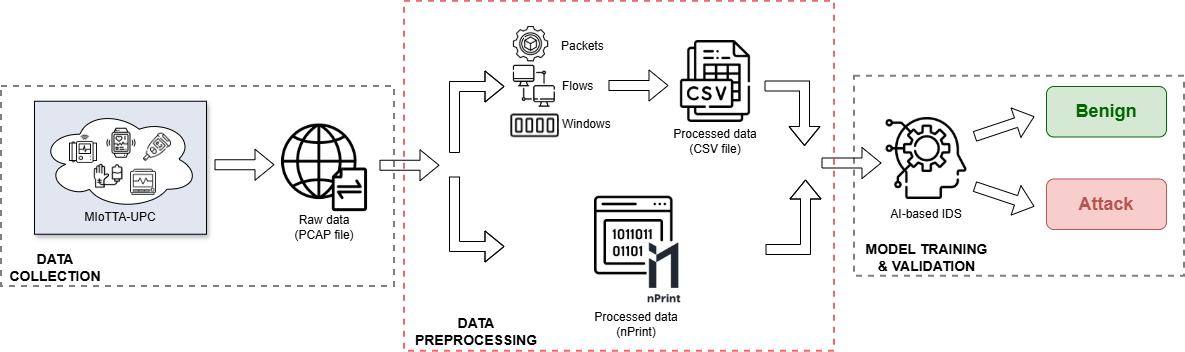
\includegraphics[width=0.85\textwidth]{miotta_npt_workflow.png}
\caption{MIOTTA-NPT tool workflow: from raw \gls{pcap} captures to structured feature datasets. The tool supports four extraction modes (packet, flow, window, combined) and two output formats (CSV, nPrint). Source:~\cite{miotta_npt_github}.}
\label{fig:miotta-workflow}
\end{figure}

The MIOTTA-NPT (Network Preprocessing Tool)~\cite{leon2025miotta, miotta_npt_github} is a configurable, open-source tool developed by the research group at UPC for transforming \gls{pcap} files into structured datasets. It occupies a central role in this thesis, as it provides the mechanism through which feature heterogeneity across datasets is resolved.

\paragraph{Architecture and modes.} The tool accepts \gls{pcap} files as input and supports two primary output formats: (i) CSV with statistical features, and (ii) nPrint binary representations. For the CSV output, four aggregation modes are available---packet, flow, window, and combined---allowing researchers to configure the extraction granularity according to their experimental needs.

\paragraph{Feature set.} In its combined mode (flow + window), the tool extracts up to 103 configurable features organized into three categories: 25 packet-level attributes, 42 flow-level statistics, and 36 window-level aggregations. These features capture a comprehensive range of traffic characteristics, including:

\begin{itemize}
    \item Connection metadata (IP addresses, ports, protocols)
    \item Packet size statistics (min, max, mean, standard deviation)
    \item Directional metrics (forward/backward packet counts, byte totals, rates)
    \item \gls{tcp} flag distributions
    \item \gls{iat} statistics
    \item Flow dynamics (covariance, variance ratio, weight, magnitude)
\end{itemize}

\paragraph{Significance for integration.} The key advantage of MIOTTA-NPT for dataset integration is its ability to process raw \gls{pcap} captures from any dataset through the same extraction pipeline, yielding identical feature spaces regardless of the source dataset. By reprocessing the \gls{pcap} files of CICIoMT2024 and IoMT-TrafficData through MIOTTA-NPT with identical configuration parameters (combined mode, window size of 100 packets), the fundamental challenge of feature heterogeneity is resolved at the source rather than through post-hoc feature mapping or engineering.

\paragraph{Comparison with existing tools.} Table~\ref{tab:tool-comparison} positions MIOTTA-NPT relative to other preprocessing tools in the literature.

\begin{table}[htbp]
\centering
\caption{Comparison of network traffic preprocessing tools~\cite{leon2025miotta}.}
\label{tab:tool-comparison}
\small
\begin{tabularx}{\textwidth}{@{}l c X p{2.2cm} c c@{}}
\toprule
\textbf{Tool} & \textbf{Year} & \textbf{Extraction Level} & \textbf{Format} & \textbf{Config.} & \textbf{\# Feat.} \\
\midrule
CICFlowMeter~\cite{cicflowmeter} & 2016 & Flow & CSV & No & 76 \\
WUSTL-EHMS~\cite{hady2020ids} & 2020 & Flow & CSV & No & 34 \\
IoT-Healthcare~\cite{hussain2021framework} & 2021 & Packet & CSV & No & 50 \\
CICIoT2023~\cite{neto2023ciciot2023} & 2023 & Flow + Window & CSV & No & 47 \\
CICIoMT2024~\cite{dadkhah2024ciciomt} & 2024 & Flow + Window & CSV & No & 45 \\
IoMT-TrafficData~\cite{areia2024iomt} & 2024 & Flow + Packet & CSV & No & 64 \\
\textbf{MIOTTA-NPT}~\cite{leon2025miotta} & \textbf{2025} & \textbf{All levels} & \textbf{CSV, nPrint} & \textbf{Yes} & \textbf{103} \\
\bottomrule
\end{tabularx}
\end{table}

% ══════════════════════════════════════════════════════════════════════════════
\section{Dataset Integration in Cybersecurity Research}
\label{sec:integration}

\subsection{The Challenge of Multi-Dataset Integration}
\label{subsec:integration-challenge}

The integration of multiple cybersecurity datasets is a recognized challenge in the research community, yet it remains underexplored. Most studies in \gls{ids} research rely on single datasets for training and evaluation, which limits the generalizability of the resulting models~\cite{domenech2025evaluating}. A comprehensive dataset-centric evaluation of federated \gls{ids} models across three IoT/IIoT datasets demonstrated that cross-dataset testing exposes substantial performance degradation---up to 30 percentage-point macro-F1 loss---when models trained on one dataset face unseen environments~\cite{abouhouran2025federated}. This finding empirically validates the necessity of multi-dataset integration for building robust detection systems.

The primary barriers to multi-dataset integration include:

\begin{enumerate}
    \item \textbf{Feature space mismatch}: Datasets extracted with different tools produce different feature sets, making direct concatenation impossible without feature engineering or re-extraction.

    \item \textbf{Semantic differences}: Even features with similar names may carry different semantics depending on the extraction methodology. For example, a ``flow duration'' computed by Zeek follows different aggregation rules than one computed by CICFlowMeter. Recent work on unified benchmarking formats has shown that such inconsistencies, together with data collection errors and duplication artifacts, are pervasive across popular \gls{nids} datasets~\cite{noblet2025nxcap}.

    \item \textbf{Label incompatibility}: Attack taxonomies and labeling conventions vary across datasets, with different granularity levels and naming schemes. Research on federated \gls{ids} has addressed this through harmonization to common family-level schemas, demonstrating that combined multi-dataset training with harmonized labels substantially restores cross-domain transfer performance~\cite{abouhouran2025federated}.

    \item \textbf{Distribution shifts}: Datasets captured in different network environments exhibit different baseline traffic distributions, which can confound model training if not properly addressed.
\end{enumerate}

\subsection{Approaches to Dataset Integration}
\label{subsec:integration-approaches}

The literature identifies several approaches to multi-dataset integration, ranging from general-purpose methodologies to domain-specific solutions:

\paragraph{General-purpose data unification.} Ali et al.~\cite{ali2015gudm} proposed the Global Unified Data Model (GUDM), a domain-independent framework for combining diverse data sources into unified datasets for learning and reasoning. Their approach employs a sequential pipeline of preprocessing methods (missing value handling, intrinsic relationship discovery, dataset reduction) followed by data modeling methods (priority-based attribute resolution, unified schema definition). A key contribution is the \textit{expert-centric priority-based} approach for resolving overlapping attributes---when multiple datasets contain semantically similar features, domain expert priorities determine which representation is preserved in the unified dataset. While developed for healthcare data, the underlying principles of systematic preprocessing, attribute conflict resolution, and unified schema generation are directly applicable to cybersecurity dataset integration.

\paragraph{PCAP-based re-extraction.} The most methodologically rigorous approach to achieving feature space unification is to reprocess raw network captures through a common extraction tool, yielding identical feature spaces by construction. Khan et al.~\cite{khan2024umnids} demonstrated this approach with the Unified Multimodal NIDS (UM-NIDS) dataset, which integrates four well-established datasets (CIC-IDS 2017, CIC-IoT 2023, UNSW-NB15, and CIC-DDoS 2019) by processing their raw \gls{pcap} files through a standardized three-stage pipeline that extracts flow-level features, packet payload information, and time-window-based contextual features. The resulting unified dataset enables cross-dataset validation and supports extensibility through the addition of new \gls{pcap} sources processed with the same tool. Complementarily, Noblet et al.~\cite{noblet2025nxcap} proposed Nxcap, a unified flow-oriented capture format for \gls{nids} benchmarking that bridges raw \gls{pcap} files and flow-level statistics. Their advanced deduplication engine revealed significant quality issues in established datasets, underscoring the importance of standardized processing pipelines that integrate data quality verification.

\paragraph{Feature-level semantic integration.} An alternative approach maps features from heterogeneous feature spaces into a common representation by identifying semantically equivalent features across datasets. This approach preserves the original feature extraction but requires careful validation that the mapped features are genuinely comparable. It is most suitable when the constituent datasets have been extracted using tools with similar underlying methodologies.

\paragraph{Federated label harmonization.} In distributed learning settings, recent work has demonstrated the effectiveness of harmonizing labels to a common family-level schema while aligning features to the intersection set across datasets~\cite{abouhouran2025federated}. Combined multi-dataset federation with harmonized labels yields approximately 90\% macro-F1 across datasets, significantly outperforming models trained on single datasets when evaluated cross-domain.

\subsection{Positioning of This Thesis}
\label{subsec:integration-positioning}

This thesis adopts a \textbf{hybrid strategy} that combines the strengths of the approaches described above. Following the PCAP-based re-extraction methodology validated by Khan et al.~\cite{khan2024umnids}, all constituent datasets are reprocessed through MIOTTA-NPT with identical configuration parameters, resolving feature heterogeneity at the source. The label harmonization follows a multi-level scheme informed by the family-level approach demonstrated in federated settings~\cite{abouhouran2025federated}, while extending it with fine-grained labels that preserve the original attack type information. The data quality assurance pipeline incorporates the preprocessing principles advocated by Ali et al.~\cite{ali2015gudm} and the deduplication awareness highlighted by Noblet et al.~\cite{noblet2025nxcap}. Finally, provenance tracking enables the cross-domain evaluation strategies whose importance has been empirically established in the recent literature~\cite{abouhouran2025federated, domenech2025evaluating}.

% ══════════════════════════════════════════════════════════════════════════════
\section{Chapter Summary and Identified Gaps}
\label{sec:gaps}

This review of the state of the art reveals the following key findings and gaps:

\begin{enumerate}
    \item \textbf{Growing threat landscape}: The \gls{iomt} domain faces an expanding array of cyber threats, with attacks increasing in both frequency and sophistication, underscoring the need for effective automated detection mechanisms.

    \item \textbf{Dataset limitations}: While several valuable benchmark datasets exist, each captures only a partial view of the threat landscape. No single dataset provides comprehensive coverage of the protocols, attack types, and device behaviors encountered in real-world \gls{iomt} deployments.

    \item \textbf{Feature heterogeneity barrier}: The use of different feature extraction tools and methodologies across datasets creates structural incompatibilities that have, to date, prevented systematic multi-dataset integration in the \gls{iomt} domain.

    \item \textbf{MIOTTA-NPT as enabler}: The availability of MIOTTA-NPT provides, for the first time, a configurable and open-source tool capable of processing raw captures from multiple datasets through a unified pipeline, resolving the feature heterogeneity barrier.

    \item \textbf{Lack of unified datasets}: No prior work has systematically integrated multiple \gls{iomt}/\gls{iot} datasets into a single, unified, \gls{ml}-ready dataset with harmonized labels and controlled provenance tracking.
\end{enumerate}

This thesis directly addresses gaps 3, 4, and 5 by leveraging MIOTTA-NPT as the foundation for a comprehensive dataset integration methodology, the design and execution of which are presented in the following chapters.

\chapter{Solution Specification and Design}
\label{ch:solution-design}

This chapter presents the detailed specification and design of the integration methodology. The approach addresses the challenges identified in the state of the art by combining standardized feature extraction through MIOTTA-NPT with a systematic multi-stage pipeline that encompasses label harmonization, data quality assurance, and provenance tracking.

% ══════════════════════════════════════════════════════════════════════════════
\section{Integration Strategy Overview}
\label{sec:strategy}

The integration strategy is structured as a multi-stage pipeline, illustrated in Figure~\ref{fig:pipeline-overview}, that transforms raw network traffic captures from multiple heterogeneous datasets into a single, unified, \gls{ml}-ready dataset. The strategy is guided by the following design principles:

\begin{enumerate}
    \item \textbf{Source-level standardization}: Feature heterogeneity is resolved at the source by reprocessing raw \gls{pcap} captures through a common tool (MIOTTA-NPT), rather than attempting post-hoc feature mapping.

    \item \textbf{Label-level harmonization}: A three-tiered labeling scheme provides classification targets at different granularity levels, enabling both broad and fine-grained intrusion detection experiments.

    \item \textbf{Provenance preservation}: Each record in the unified dataset retains explicit attribution to its source dataset, enabling cross-domain evaluation and analysis of per-source model performance.

    \item \textbf{Quality-first processing}: Data quality assurance is integrated as a core pipeline stage, not an afterthought, ensuring that missing values, outliers, and distribution anomalies are systematically addressed.

    \item \textbf{Extensibility}: The pipeline is designed to accommodate additional datasets (e.g., future custom datasets from the MIoTTA-UPC testbed) without requiring architectural modifications.
\end{enumerate}

\begin{figure}[htbp]
\centering
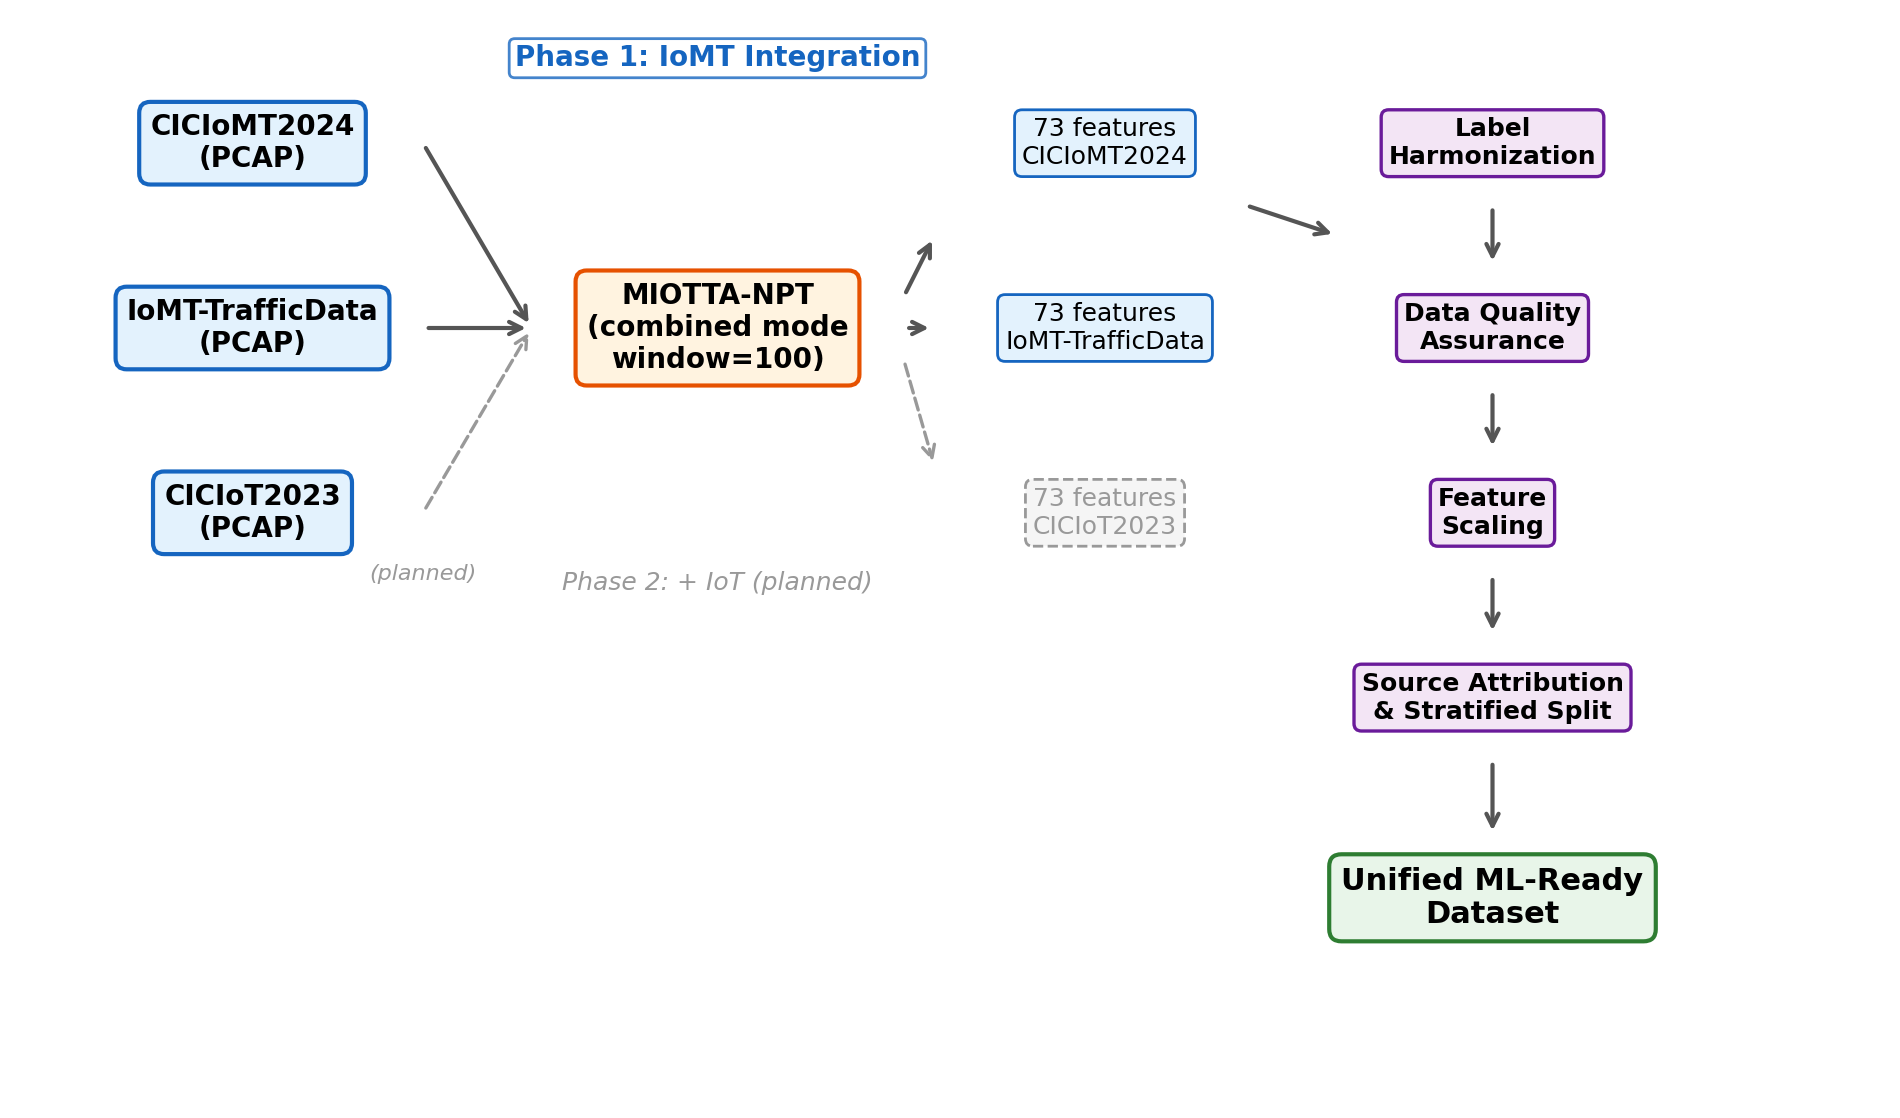
\includegraphics[width=\textwidth]{pipeline_overview.png}
\caption{Overview of the multi-stage integration pipeline. Raw packet captures from CICIoMT2024 and IoMT-TrafficData are processed through MIOTTA-NPT with identical configuration, yielding standardized 73-feature representations. These are then passed through the integration pipeline stages (label harmonization, data quality assurance, feature scaling, and stratified splitting) to produce the final unified ML-ready dataset.}
\label{fig:pipeline-overview}
\end{figure}

% ══════════════════════════════════════════════════════════════════════════════
\section{Dataset Selection and Justification}
\label{sec:dataset-selection}

The selection of datasets for integration is driven by three criteria: (i)~domain relevance to \gls{iomt} security, (ii)~complementarity in attack coverage, and (iii)~availability of raw \gls{pcap} captures for reprocessing. Table~\ref{tab:selection-criteria} summarizes how each dataset meets these criteria.

\begin{table}[htbp]
\centering
\caption{Dataset selection criteria evaluation.}
\label{tab:selection-criteria}
\small
\begin{tabularx}{\textwidth}{@{}l c c X@{}}
\toprule
\textbf{Dataset} & \textbf{Domain} & \textbf{PCAP} & \textbf{Complementary Coverage} \\
\midrule
CICIoMT2024 & IoMT & \checkmark & Multi-protocol IoMT attacks (18 types) \\
IoMT-TrafficData & IoMT & \checkmark & Hospital testbed attacks, data malformation \\
HospNet26 & Real hospital & \checkmark & Real clinical traffic (benign only) — generalization probe \\
\bottomrule
\end{tabularx}
\end{table}

The integration focuses on the two \gls{iomt}-specific datasets:

\begin{itemize}
    \item \textbf{Phase~1 (IoMT integration):} Integrates CICIoMT2024 and IoMT-TrafficData, which share a common \gls{iomt} domain focus, yielding a unified dataset with diverse attack coverage. The resulting artifact is published for community reuse~\cite{unified_iomt_csuc2026}.
\end{itemize}

Additionally, the trained models are evaluated on HospNet26 real hospital network traffic as an out-of-distribution generalization test, without any retraining or adaptation.

% ══════════════════════════════════════════════════════════════════════════════
\section{Feature Standardization via MIOTTA-NPT}
\label{sec:feature-standardization}

\subsection{Processing Configuration}
\label{subsec:processing-config}

All datasets are processed through MIOTTA-NPT using an identical configuration to ensure strict feature space alignment:

\begin{itemize}
    \item \textbf{Mode}: Combined (flow + window), which provides the richest feature representation by capturing both per-flow statistics and window-level temporal aggregations.
    \item \textbf{Window size}: 100 packets, providing a balance between temporal context and computational tractability.
    \item \textbf{Feature set}: The full set of combined-mode features, yielding 73 features per record (the subset of the 103 total features that applies to the combined mode).
\end{itemize}

The choice of the combined mode is motivated by several factors: (i)~it captures both flow-level semantics (who is communicating, how much data is exchanged) and window-level temporal patterns (traffic behavior over a fixed packet window), (ii)~it provides a sufficiently rich feature space for diverse \gls{ml} architectures, and (iii)~the resulting feature count (73) is manageable for both traditional and deep learning models.

\subsection{Resulting Feature Space}
\label{subsec:feature-space}

After processing through MIOTTA-NPT, each dataset produces records with an identical set of 73 features. These features can be organized into the following functional groups:

\begin{enumerate}
    \item \textbf{Connection metadata} (5 features): Flow identifier, window number, protocol type, IP-related fields.
    \item \textbf{Packet size statistics} (6 features): Minimum, maximum, mean, and standard deviation of packet lengths; total bytes; total packet size.
    \item \textbf{Directional metrics} (14 features): Forward/backward packet counts, byte totals, payload sizes, header sizes, and per-second rates.
    \item \textbf{Flow dynamics} (6 features): Rate, source/destination rates, magnitude, radius, covariance, variance ratio.
    \item \textbf{TCP flag distributions} (12 features): Counts and ratios of SYN, ACK, FIN, RST, PSH, ECE, CWR, and URG flags.
    \item \textbf{Temporal features} (6 features): Forward/backward/flow inter-arrival times, timestamps.
    \item \textbf{Protocol indicators} (14 features): Binary or count indicators for HTTP, HTTPS, DNS, TCP, UDP, ARP, ICMP, SSH, SMTP, IRC, DHCP, Telnet, LLC, IGMP, IPv4.
    \item \textbf{Window-level aggregations} (10 features): Header length, TTL, inter-arrival time at window level, initial RTT, connection state indicators.
\end{enumerate}

The strict identity of the feature spaces across datasets---verified empirically as described in Chapter~\ref{ch:execution}---eliminates the need for any feature mapping or alignment procedures.

\subsection{Progressive Deployment of MIOTTA-NPT}
\label{subsec:progressive-miotta}

The pipeline is designed to be agnostic to the number of input datasets: adding a new MIOTTA-processed dataset requires only the creation of a corresponding label mapping (Section~\ref{sec:label-harmonization}) and its inclusion in the concatenation stage. This extensibility also accommodates future datasets generated from the MIoTTA-UPC testbed under development at the university.

% ══════════════════════════════════════════════════════════════════════════════
\section{Integration Architecture}
\label{sec:two-phase}

\subsection{Phase 1: IoMT Semantic Integration}
\label{subsec:phase1}

Phase~1 focuses on the integration of the two \gls{iomt}-specific datasets (CICIoMT2024 and IoMT-TrafficData), both of which have been processed through MIOTTA-NPT with identical configuration. Since the MIOTTA-NPT processing guarantees structural compatibility at the feature level, the integration effort in this phase concentrates on:

\begin{enumerate}
    \item \textbf{Cross-dataset feature verification}: Confirming that the MIOTTA-processed datasets share identical column names, data types, and value ranges.
    \item \textbf{Label harmonization}: Mapping the different attack labels from each dataset into a unified three-level labeling scheme (Section~\ref{sec:label-harmonization}).
    \item \textbf{Data quality normalization}: Applying consistent missing value treatment, infinity value handling, and zero-variance feature removal across both datasets.
    \item \textbf{Source attribution}: Adding a provenance column to track the origin of each record.
\end{enumerate}

The \textit{semantic} nature of this phase refers to the careful attention paid to ensuring that the mapped labels carry consistent meaning across the integrated dataset, and that any dataset-specific characteristics (e.g., NaN values in TCP flag features for non-TCP traffic) are understood and handled consistently.

% ══════════════════════════════════════════════════════════════════════════════
\section{Label Harmonization}
\label{sec:label-harmonization}

The absence of a common labeling convention across datasets necessitates a systematic harmonization procedure. This thesis defines a three-level labeling hierarchy, each level serving a distinct analytical purpose:

\subsection{Three-Level Labeling Scheme}
\label{subsec:label-levels}

\begin{description}
    \item[Level 1 --- Binary (\texttt{label\_binary}):] Classifies each record as either \texttt{Benign} or \texttt{Attack}. This level is useful for basic intrusion detection (is there an attack?) and provides the most balanced class distribution.

    \item[Level 2 --- Category (\texttt{label\_category}):] Groups attack types into six operational categories used in this thesis: \texttt{Benign}, \texttt{DDoS}, \texttt{DoS}, \texttt{MQTT}, \texttt{Reconnaissance}, and \texttt{Spoofing}. The operational mapping adopts a dedicated \texttt{MQTT} category: all MQTT-related attacks (\texttt{MQTT-DDoS-*}, \texttt{MQTT-DoS-*}, \texttt{MQTT-Malformed\_Data}, and \texttt{MQTT Malaria}) are grouped under \texttt{MQTT}. The remaining categories retain nature-based semantics. This level supports multi-class classification at a practical operational level, enabling security analysts to understand both attack nature and protocol-oriented behavior.

    \item[Level 3 --- Fine-grained (\texttt{label\_fine}):] Preserves the original attack type labels from each dataset (e.g., \texttt{DDoS\_TCP\_Flood}, \texttt{ARP\_Spoofing}), with normalization applied to ensure consistent formatting. This level enables the most detailed analysis but may exhibit significant class imbalance due to the uneven representation of specific attack types across datasets.
\end{description}

\subsection{Mapping Strategy}
\label{subsec:label-mapping}

For each dataset, an explicit mapping dictionary defines the correspondence between the original labels and the three harmonized levels. These mappings are developed based on:

\begin{itemize}
    \item The attack type descriptions provided in the original dataset publications~\cite{dadkhah2024ciciomt, areia2024iomt}.
    \item Analysis of the attack execution methodologies described by the dataset authors.
    \item Consultation with the thesis advisors to resolve ambiguous cases where an attack type could plausibly belong to multiple categories.
\end{itemize}

The mapping dictionaries are maintained as configuration artifacts within the integration pipeline, enabling transparent auditing and modification as needed.

% ══════════════════════════════════════════════════════════════════════════════
\section{Data Quality Assurance}
\label{sec:quality}

Data quality issues, if unaddressed, can introduce noise, bias, or artifacts into the unified dataset. The pipeline incorporates the following quality assurance procedures:

\begin{enumerate}
    \item \textbf{Missing value treatment}: Features with NaN values (e.g., TCP flag statistics for windows containing only non-TCP traffic) are imputed with 0 when the NaN arises from the absence of the relevant protocol, or flagged for removal if the missingness rate exceeds a configurable threshold.

    \item \textbf{Infinity value handling}: Infinite values, typically arising from division by zero in rate or ratio computations, are replaced with the maximum finite value of the respective feature column.

    \item \textbf{Zero-variance feature removal}: Features that exhibit no variation across the entire integrated dataset are removed, as they carry no discriminative information.

    \item \textbf{Near-zero-variance detection}: Features with extremely low variance are flagged for review, as they may add noise without contributing to model performance.

    \item \textbf{Duplicate removal}: Exact duplicate rows are identified and removed to prevent artificial inflation of certain traffic patterns.

    \item \textbf{Type consistency}: All numeric features are cast to consistent data types (\texttt{float32} or \texttt{float64}) across datasets to prevent type-related processing errors.
\end{enumerate}

% ══════════════════════════════════════════════════════════════════════════════
\section{Feature Scaling}
\label{sec:scaling}

After concatenation and quality assurance, feature scaling is applied to normalize the value ranges across the unified dataset. The primary motivation is that features from different datasets, even when representing the same physical quantity, may exhibit different value ranges due to differences in network traffic volumes, packet sizes, or timing characteristics.

For this thesis, the Phase~1 integration pipeline adopts a single scaling strategy throughout: \textbf{standardization} ($z$-score normalization) implemented with scikit-learn's \texttt{StandardScaler}. For each feature, the scaler subtracts the mean and divides by the standard deviation computed \textbf{only on the training partition}, then applies the same transformation to the validation and test partitions. The fitted scaler is persisted (\texttt{scaler.joblib}) so that inference and any future experiments reuse identical preprocessing. This choice matches the implementation in Chapter~\ref{ch:execution} and in the exported CSV splits used for model training.

Alternative schemes such as min--max scaling to $[0,1]$ are \textit{not} used in the current work: they were considered only at the design stage; the final pipeline commits to z-score standardization for consistency with gradient-based and distance-based learners and to avoid compressing heavy-tailed traffic features into a bounded interval in a way that could distort relative magnitudes.

Feature scaling is applied \textit{after} the train/validation/test split. Computing scaling parameters exclusively on the training partition prevents information leakage from the validation and test sets.

% ══════════════════════════════════════════════════════════════════════════════
\section{Dataset Provenance and Source Attribution}
\label{sec:provenance}

Each record in the unified dataset includes a \texttt{source} column that identifies its dataset of origin (e.g., \texttt{CICIoMT2024}, \texttt{IoMT-TrafficData}). This simple but critical mechanism enables several advanced evaluation strategies:

\begin{itemize}
    \item \textbf{Cross-domain evaluation}: Models can be trained on one or more source datasets and tested on held-out data from a different source, directly measuring cross-domain generalizability.
    \item \textbf{Source-stratified analysis}: Performance metrics can be disaggregated by source dataset, revealing whether a model's overall accuracy masks poor performance on a specific data domain.
    \item \textbf{Leave-one-source-out validation}: A dataset can be entirely excluded from training and used exclusively for testing, simulating deployment in a novel environment.
\end{itemize}

% ══════════════════════════════════════════════════════════════════════════════
\section{Stratified Splitting Strategy}
\label{sec:splitting}

The unified dataset is partitioned into training, validation, and test sets using a stratified splitting approach that preserves both the label distribution and the source distribution in each partition. Concretely, the stratification key is the combination of \texttt{label\_category} and \texttt{source}, ensuring that:

\begin{itemize}
    \item Each attack category is represented proportionally in all partitions.
    \item Each source dataset contributes proportionally to all partitions.
    \item Rare attack types from specific sources are not entirely lost to a single partition.
\end{itemize}

The default split ratios are 70\% training, 15\% validation, and 15\% testing, configurable through pipeline parameters.

% ══════════════════════════════════════════════════════════════════════════════
\section{Chapter Summary}
\label{sec:design-summary}

This chapter has presented the complete specification and design of the dataset integration methodology. The key design decisions are:

\begin{enumerate}
    \item \textbf{MIOTTA-NPT as the unification backbone}: Processing all datasets through the same tool with identical configuration eliminates feature heterogeneity at the source.
    \item \textbf{Three-level label harmonization}: Multiple classification granularities support diverse experimental setups.
    \item \textbf{Provenance tracking}: Source attribution enables rigorous cross-domain evaluation.
    \item \textbf{Quality-integrated pipeline}: Data quality assurance is embedded as a core pipeline stage.
\end{enumerate}

The following chapter describes the execution of this pipeline, presenting the empirical findings from each stage and the characteristics of the resulting unified dataset.

\chapter{Development of the Integration Pipeline}
\label{ch:execution}

This chapter describes the development and execution of each stage of the integration pipeline designed in Chapter~\ref{ch:solution-design}. The presentation follows the chronological order in which the work was carried out: first, the exploratory analysis of the original datasets; then, the examination of the MIOTTA-NPT processed versions; and finally, the execution of the integration pipeline that produces the unified dataset.

% ══════════════════════════════════════════════════════════════════════════════
\section{Exploratory Analysis of Original Datasets}
\label{sec:eda-original}

Before proceeding with the integration, each dataset was subjected to comprehensive exploratory data analysis in its original feature representation. This step served to understand the structure, content, and quality of each source, and to identify characteristics that would inform the subsequent integration decisions.

\subsection{CICIoMT2024 --- Original Feature Space}
\label{subsec:eda-ciciomt}

The CICIoMT2024 dataset, introduced by Dadkhah et al.~\cite{dadkhah2024ciciomt}, was created by the Canadian Institute for Cybersecurity specifically for evaluating the security of IoMT devices. The experimental testbed comprised 40 IoMT devices (25 real and 15 simulated via IoTFlock), with attacks executed by four Raspberry Pi units across WiFi and MQTT protocols. Features were extracted from raw PCAP files using a DPKT-based window aggregation pipeline---the same extraction methodology employed for CICIoT2023.

The exploratory analysis revealed the following characteristics:

\begin{itemize}
    \item \textbf{Scale}: 8,322,896 records (6,708,714 training, 1,614,182 test), each described by 45 features. The dataset occupies approximately 5.1~GB in memory.
    \item \textbf{Feature space}: All 45 features are numeric (\texttt{float64}), comprising packet/flow statistics (Header\_Length, Rate, Tot\_size, IAT), protocol indicator flags (HTTP, DNS, TCP, UDP, MQTT), and TCP flag counts. Notably, the \texttt{Duration} column actually encodes TTL (Time-To-Live) values (range 0--255), not time duration---a critical observation for correct interpretation.
    \item \textbf{Attack taxonomy}: 18 distinct attack types organized into 5 categories---DDoS (4~types, 66.6\%), DoS (4~types, 26.7\%), MQTT (5~types, 3.3\%), Reconnaissance (4~types, 1.6\%), and Spoofing (1~type, 0.2\%)---plus Benign traffic (1.6\%). The 5 MQTT-specific attacks (DDoS/DoS Connect and Publish Flood, Malformed Data) are unique to this dataset and not present in CICIoT2023.
    \item \textbf{Class imbalance}: Substantial, with a maximum-to-minimum ratio of approximately 2,157:1 between DDoS variants and Spoofing. At the binary level, attack traffic constitutes 98.4\% of records.
    \item \textbf{Data quality}: Minimal issues---only 148 missing values (in the Weight and Variance features), no infinite values, and 7,216 duplicate rows (0.09\%).
\end{itemize}

\subsection{IoMT-TrafficData --- Original Feature Space}
\label{subsec:eda-iomt-traffic}

The IoMT-TrafficData dataset, introduced by Areia et al.~\cite{areia2024iomt}, provides network traffic from a hospital-oriented IoMT testbed with 10+ medical devices communicating over CoAP, MQTT, and HTTP protocols. Unlike the CIC datasets, features were extracted using \textbf{Zeek} (formerly Bro), a flow-oriented network analysis framework that produces per-connection records rather than window-based aggregations.

The exploratory analysis revealed characteristics fundamentally different from CICIoMT2024:

\begin{itemize}
    \item \textbf{Scale}: 969,141 flow records described by 101 features (88 numeric, 13 categorical/string). The dataset is considerably smaller than CICIoMT2024 but provides complementary attack coverage.
    \item \textbf{Feature space}: The 101 Zeek-derived features are organized into functional groups---connection metadata (15 features), Zeek base statistics (6), flow duration and rates (6), forward packet statistics (20), backward packet statistics (20), flow-level packet statistics (11), inter-arrival times (7), active/idle periods (4), bulk transfer metrics (6), and TCP window sizes (6). This schema is semantically richer than the CIC window-based features but structurally incompatible: direct column-matching between the two schemas is not possible.
    \item \textbf{Attack taxonomy}: 8 attack types plus Benign traffic---ARP Spoofing, Apache Killer (DoS), CAM Table Overflow, MQTT Malaria (MQTT flooding), Reconnaissance (Netscan), R-U-Dead-Yet/RUDY (slow POST), Slow Loris (slow HTTP), and Slow Read (slow read DoS). Several of these overlap with CICIoMT2024 attacks (ARP Spoofing, Reconnaissance, DoS variants), enabling cross-dataset label harmonization.
    \item \textbf{Class imbalance}: Moderate, with a maximum-to-minimum ratio of approximately 22:1---significantly less extreme than CICIoT2023 but still requiring attention during model training.
    \item \textbf{Data quality}: No missing values and no infinite values in the original data. However, 8 features exhibited zero variance and 17 had near-zero variance (>95\% identical values), indicating that a substantial portion of the feature space carries minimal discriminative information. Additionally, 36 features showed high skewness ($|s| > 5$), and 6,434 duplicate rows (0.66\%) were identified.
    \item \textbf{Integration implication}: The fundamental difference between the Zeek flow-level schema and the DPKT window-based schema used by the CIC datasets confirmed that semantic feature mapping alone would be insufficient for reliable integration. This observation was a primary motivation for adopting MIOTTA-NPT as the unifying feature extraction tool, as it can reprocess the raw PCAPs from all datasets into a common representation.
\end{itemize}

\subsection{CICIoT2023 --- Original Feature Space}
\label{subsec:eda-ciciot}

The CICIoT2023 dataset, introduced by Neto et al.~\cite{neto2023ciciot2023}, represents the largest-scale IoT attack dataset employed in this work. It was generated in a realistic smart-home topology comprising 105 IoT devices (67 directly involved, 38 Zigbee/Z-Wave peripherals), with 7 Raspberry Pi units orchestrating attacks. Feature extraction followed the same DPKT window-based aggregation pipeline as CICIoMT2024, establishing structural compatibility between the two CIC datasets.

The exploratory analysis revealed:

\begin{itemize}
    \item \textbf{Scale}: 44,763,144 records distributed across 63 CSV files (\(\sim\)9.1~GB), each record described by 39 features plus a label column (40 columns total). This makes it the largest dataset by an order of magnitude.
    \item \textbf{Feature space}: 39 features---38 \texttt{float64} and 1 \texttt{int64} (Protocol Type). The feature set largely overlaps with CICIoMT2024 (same extraction methodology), although 7 features documented in the paper (including \texttt{flow\_duration}, \texttt{Srate}, \texttt{Drate}, \texttt{urg\_count}, \texttt{Magnitue}, \texttt{Radius}, \texttt{Covariance}) are absent from the actual CSV files, while \texttt{IGMP} and \texttt{Time\_To\_Live} appear as extras. This discrepancy between the published schema and the distributed data was an important finding.
    \item \textbf{Attack taxonomy}: 33 distinct attack types organized into 7 categories---DDoS (12~types, \(\sim\)34M records), DoS (4~types, \(\sim\)8.1M), Mirai (3~types, \(\sim\)2.6M), Benign (\(\sim\)1.1M), Spoofing (2~types, \(\sim\)0.5M), Reconnaissance (5~types, \(\sim\)0.35M), Web-based (6~types, \(\sim\)25K), and Brute Force (1~type, \(\sim\)13K). The Mirai, Web-based, and Brute Force categories are exclusive to this dataset and not found in the IoMT-specific sources.
    \item \textbf{Class imbalance}: Extreme, with a maximum-to-minimum ratio of approximately 5,750:1 between DDOS-ICMP\_FLOOD (6.85M records) and UPLOADING\_ATTACK (1,192 records). At the binary level, 97.7\% of records represent attack traffic.
    \item \textbf{Data quality}: 35 infinity values (concentrated in the Rate feature, replaced with NaN), 1,803,394 missing values after replacement, and a high duplicate rate of 33.33\% in the analyzed sample. The elevated duplication is attributable to the window-based aggregation methodology, where consecutive windows of identical packet patterns produce identical feature vectors.
    \item \textbf{Window aggregation bias}: Different attack categories use different window sizes---10 packets for low-volume attacks (Web-based, Reconnaissance, Spoofing, Benign, Brute Force) and 100 packets for high-volume attacks (DDoS, DoS, Mirai). This introduces a systematic methodological difference across categories that must be considered when interpreting per-category results.
\end{itemize}

\subsection{Key Observations from Original Analyses}
\label{subsec:eda-summary}

A critical finding from the exploratory analyses is the fundamental structural incompatibility across the three datasets. As illustrated in Figure~\ref{fig:feature-count-comparison}, each dataset was originally extracted using a different tool and yields a different number of features: CICIoMT2024 provides 45 features (CIC internal tool), IoMT-TrafficData provides 101 features (Zeek), and CICIoT2023 provides 47 features (CIC internal tool). Beyond the numerical difference, the features carry different semantics---Zeek operates at the flow level with a distinct aggregation logic compared to the CIC window-based approach. This incompatibility confirmed the necessity of re-extracting all datasets through MIOTTA-NPT to achieve a unified feature space.

\begin{figure}[htbp]
\centering
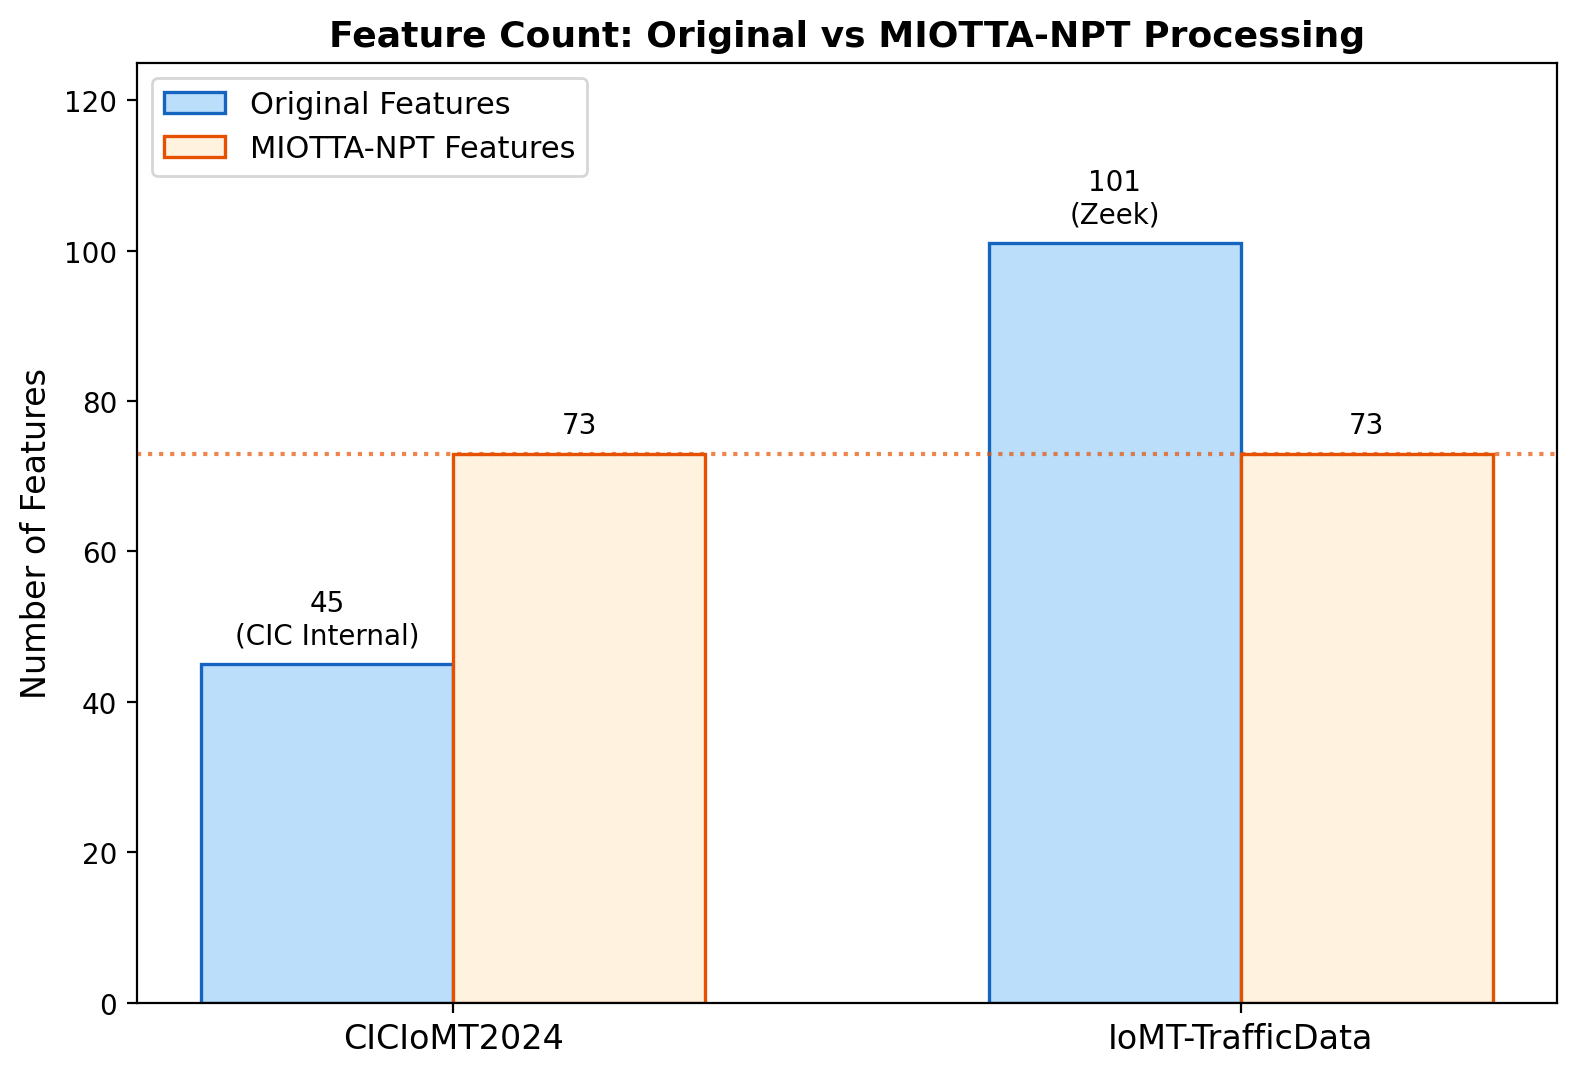
\includegraphics[width=0.85\textwidth]{feature_count_comparison.png}
\caption{Comparison of original feature counts across the three datasets versus the standardized 73-feature space produced by MIOTTA-NPT. The dashed bar for CICIoT2023 indicates that its MIOTTA-NPT processing is planned for Phase~2. The horizontal dotted line marks the unified target of 73 features.}
\label{fig:feature-count-comparison}
\end{figure}

% ══════════════════════════════════════════════════════════════════════════════
\section{MIOTTA-NPT Feature Extraction Results}
\label{sec:miotta-results}

This section presents the results of processing the available datasets through MIOTTA-NPT, verifying that the tool produces the expected standardized feature space and examining the characteristics of the resulting data. Figure~\ref{fig:dataset-summary} provides an overview of the two MIOTTA-processed datasets.

\begin{figure}[htbp]
\centering
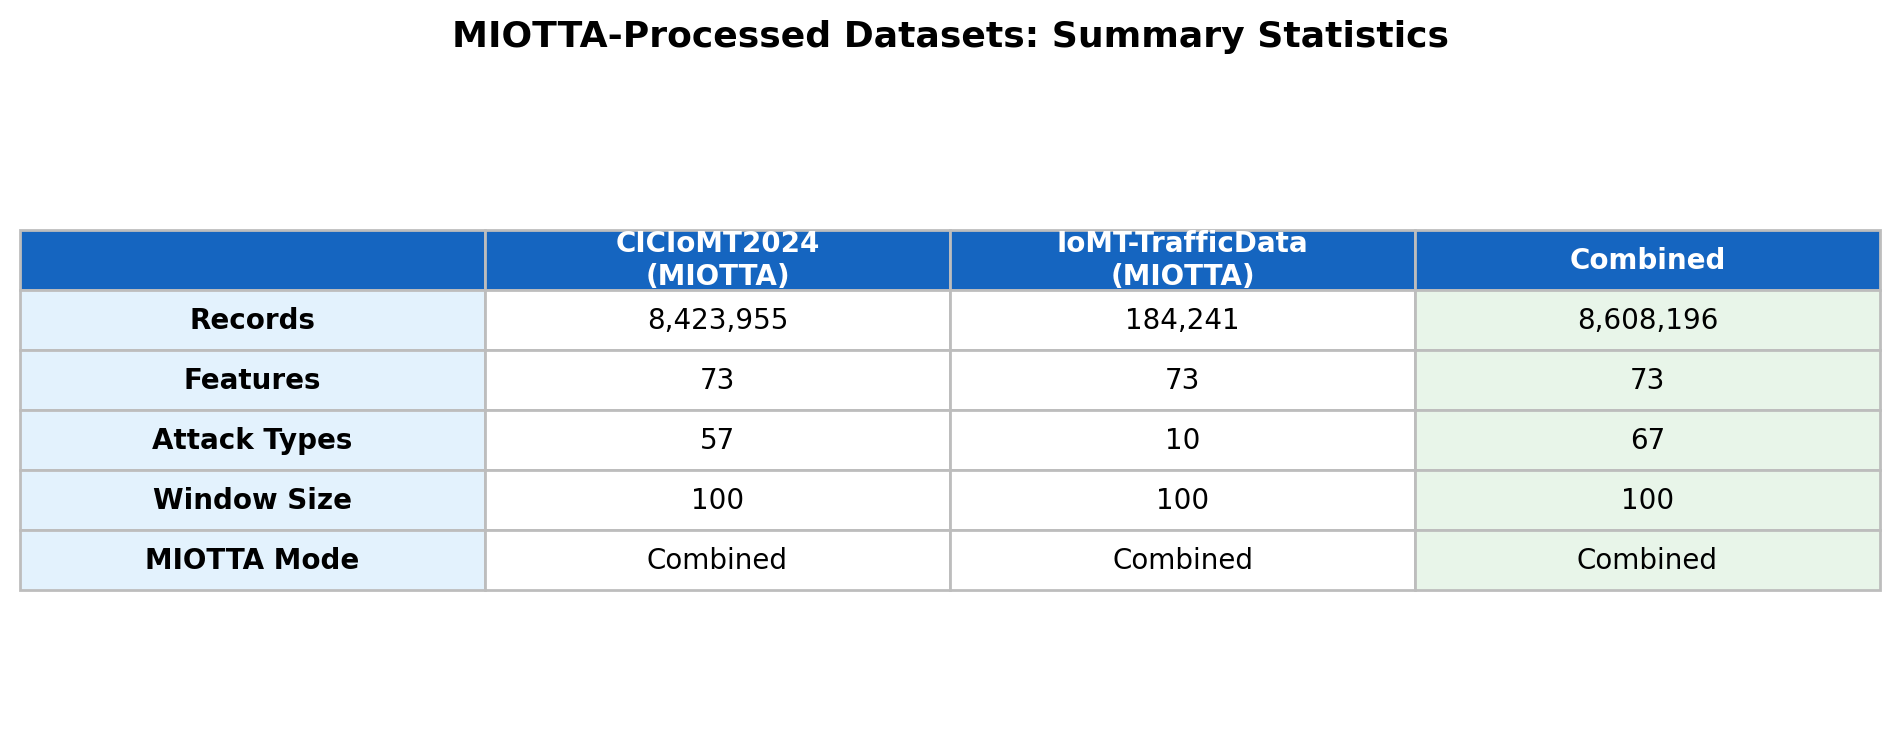
\includegraphics[width=0.85\textwidth]{dataset_summary_table.png}
\caption{Summary statistics of the two MIOTTA-processed datasets. Both datasets share an identical 73-feature space extracted in combined mode with a window size of 100 packets.}
\label{fig:dataset-summary}
\end{figure}

\subsection{CICIoMT2024 --- MIOTTA-Processed}
\label{subsec:miotta-ciciomt}

The MIOTTA-NPT processing of CICIoMT2024 yielded 8,423,955 records (6,872,287 train and 1,551,668 test) across 73 features, covering all 18 original attack types plus benign traffic. Figure~\ref{fig:ciciomt-attack-dist} shows the distribution of records across attack types, revealing significant class imbalance---a characteristic inherited from the original dataset that the integration pipeline must address.

\begin{figure}[htbp]
\centering
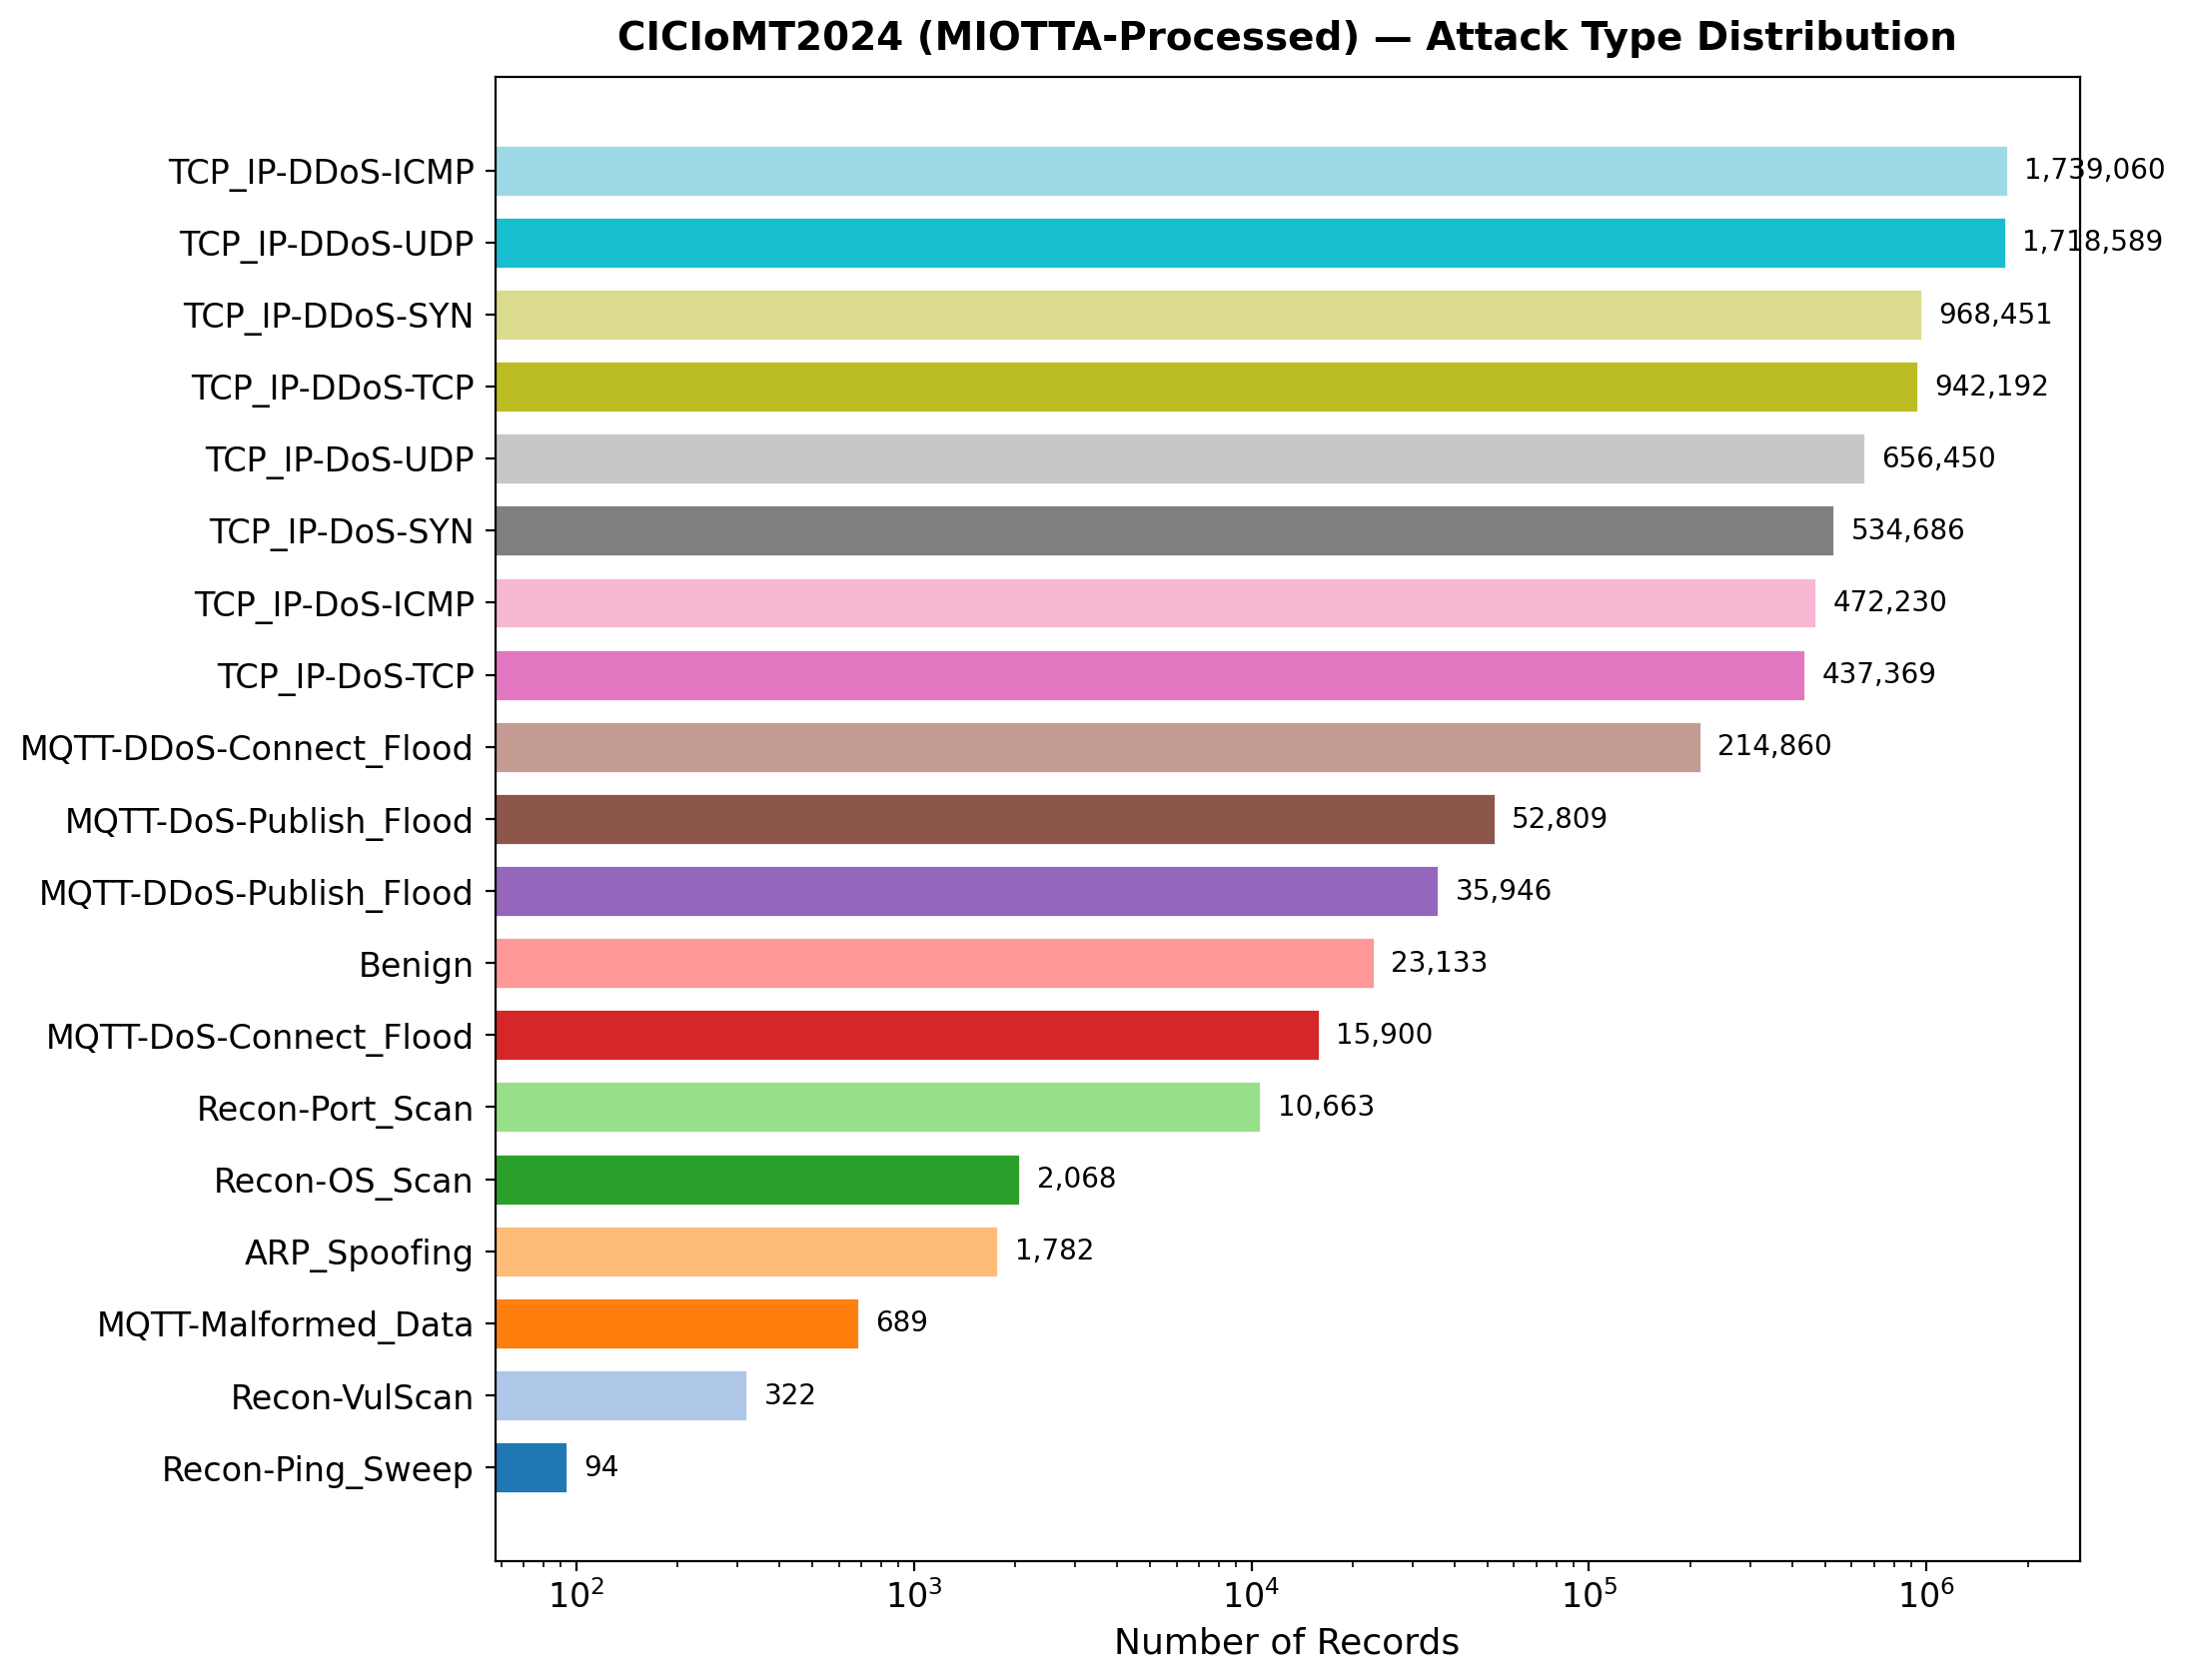
\includegraphics[height=0.86\textheight, keepaspectratio]{ciciomt2024_miotta_attack_dist.png}
\caption{Attack type distribution in the MIOTTA-processed CICIoMT2024 dataset. The logarithmic scale reveals the substantial class imbalance, with certain attack types (e.g., DDoS variants) having orders of magnitude more records than others.}
\label{fig:ciciomt-attack-dist}
\end{figure}

\subsection{IoMT-TrafficData --- MIOTTA-Processed}
\label{subsec:miotta-iomt-traffic}

The MIOTTA-NPT processing of IoMT-TrafficData produced 184,241 records across the same 73 features. Figure~\ref{fig:iomt-attack-dist} shows the attack type distribution. Compared to CICIoMT2024, this dataset is considerably smaller but provides complementary attack coverage, particularly in categories such as Apache Killer, CAM Table Overflow, and RUDY that are not present in CICIoMT2024.

\begin{figure}[htbp]
\centering
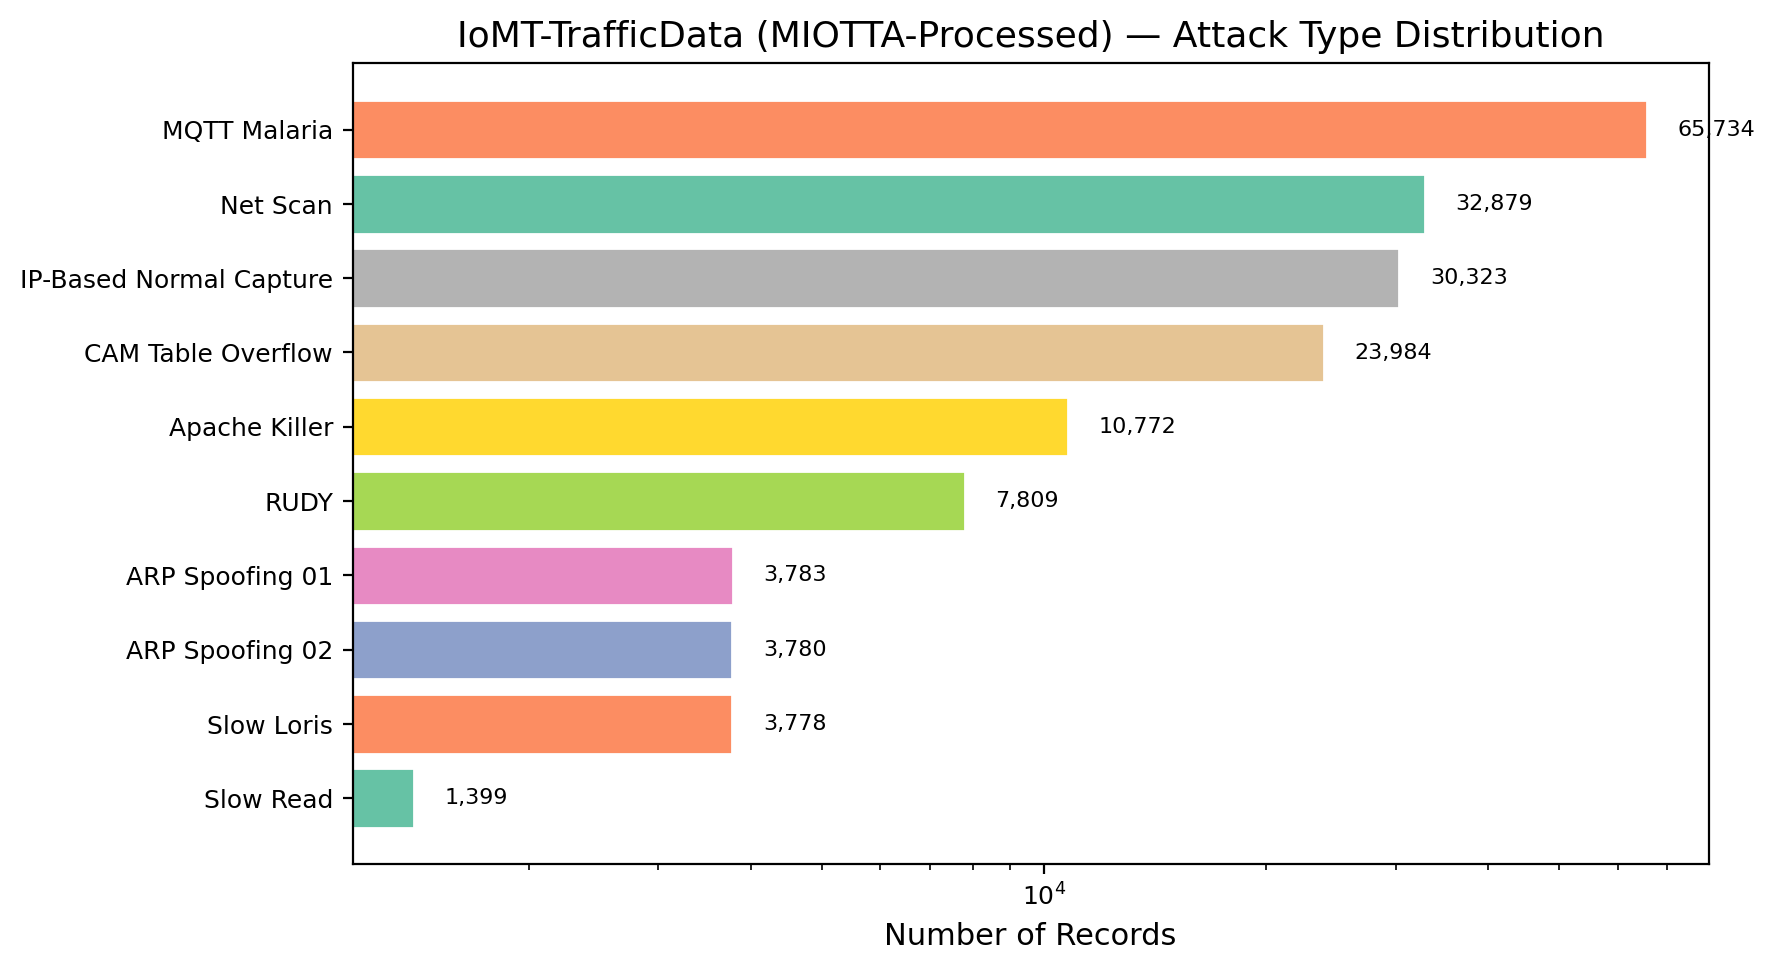
\includegraphics[width=0.85\textwidth]{iomt_traffic_miotta_attack_dist.png}
\caption{Attack type distribution in the MIOTTA-processed IoMT-TrafficData dataset. The dataset contains 10 traffic categories including benign traffic and 9 attack types relevant to IoMT environments.}
\label{fig:iomt-attack-dist}
\end{figure}

\subsection{Cross-Dataset Feature Verification}
\label{subsec:feature-verification}

A fundamental prerequisite for the integration is that both MIOTTA-processed datasets share an identical feature space. This was verified empirically, as shown in Figure~\ref{fig:feature-verification}: both datasets produce exactly 73 columns with identical names and data types, confirming that MIOTTA-NPT resolves the feature heterogeneity problem at the source.

\begin{figure}[htbp]
\centering
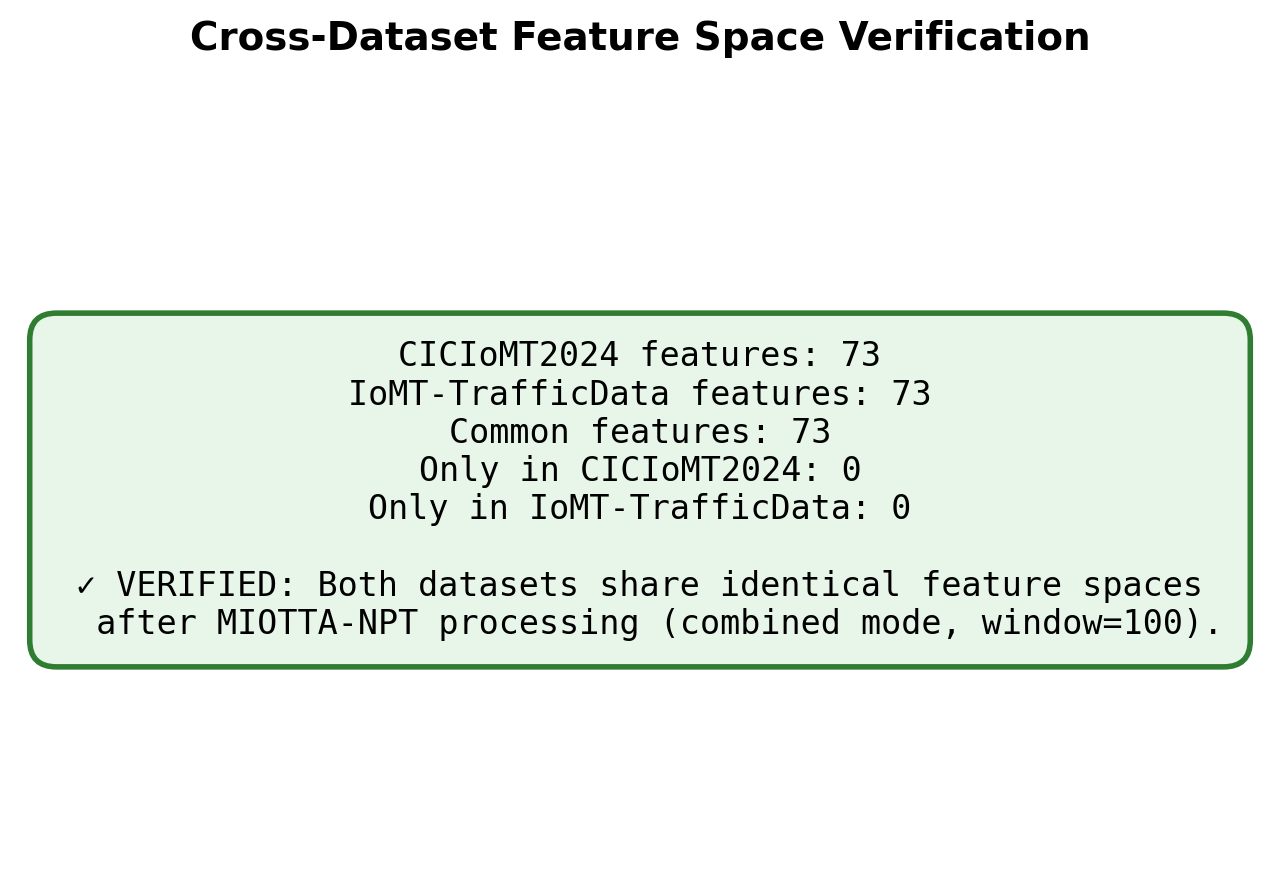
\includegraphics[width=0.7\textwidth]{feature_verification.png}
\caption{Cross-dataset feature space verification. The comparison confirms that both MIOTTA-processed datasets share an identical set of 73 features, with no dataset-exclusive columns.}
\label{fig:feature-verification}
\end{figure}

While the feature names are identical, the value distributions differ across datasets---reflecting genuine differences in network traffic characteristics. Figure~\ref{fig:feature-distributions} presents the distributions of eight key features across both datasets, revealing notable differences in value ranges and distribution shapes. These differences are expected and desirable, as they represent the diversity of network environments that the unified dataset aims to capture.

\begin{figure}[htbp]
\centering
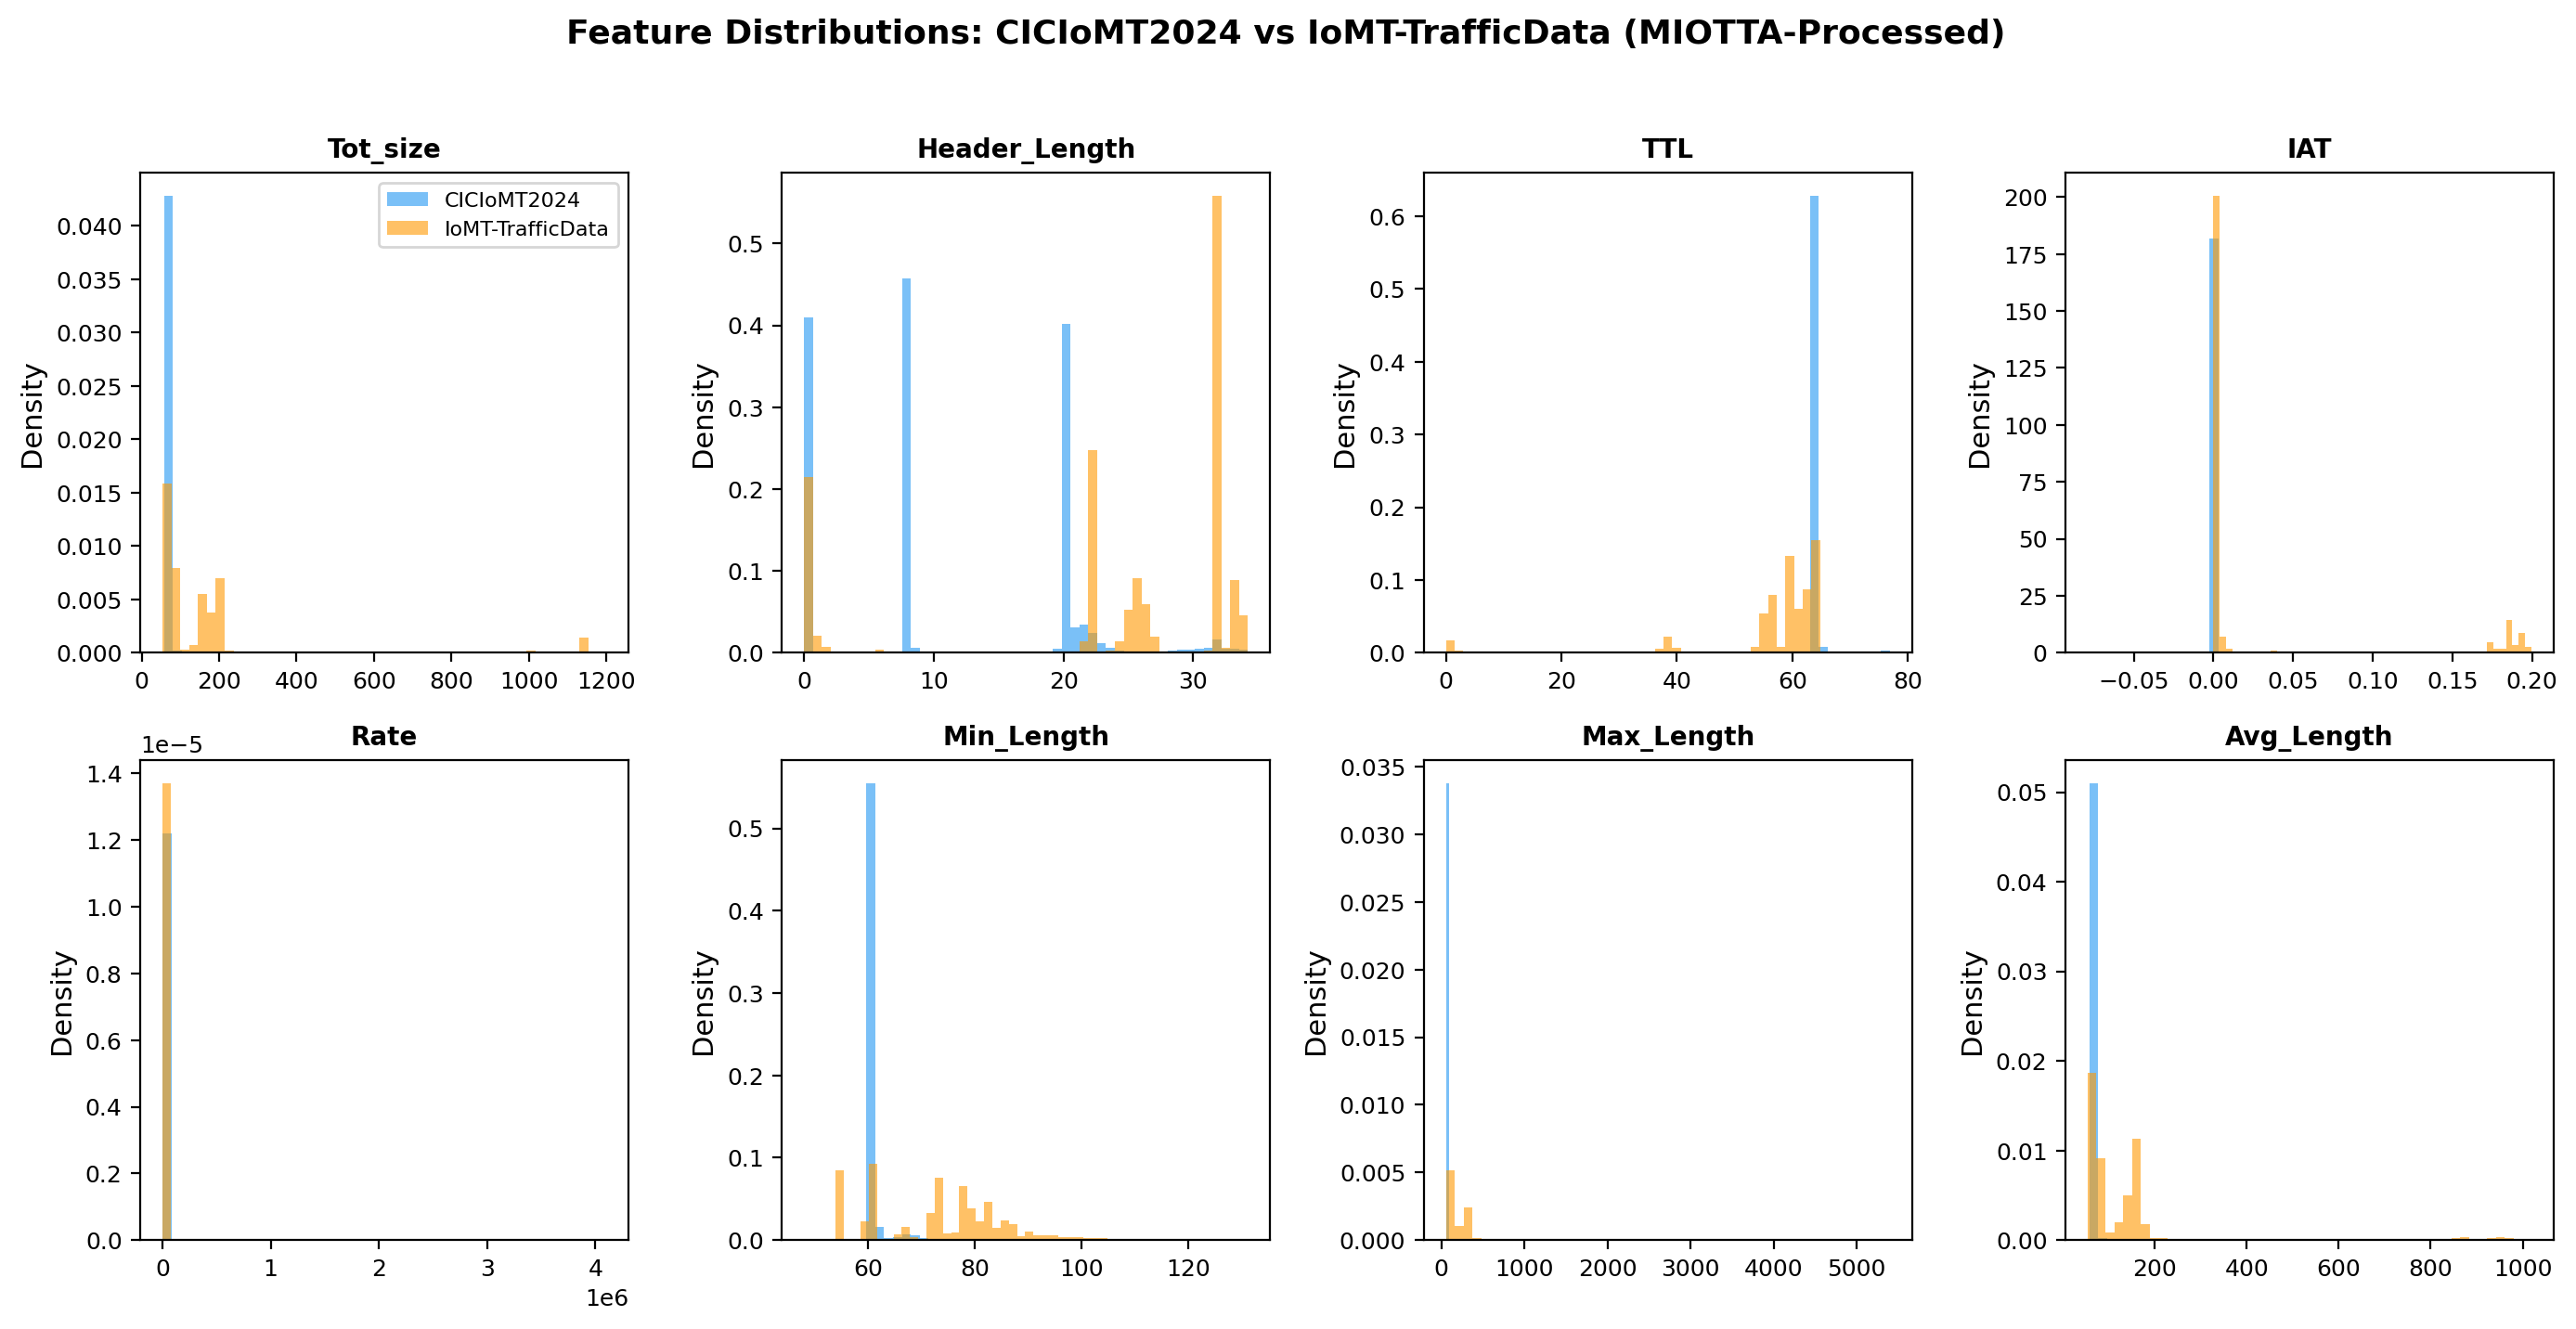
\includegraphics[width=\textwidth]{feature_distributions_comparison.png}
\caption{Distribution comparison of key features across the two MIOTTA-processed datasets (99th percentile clipping applied for visualization). The differences in distributions reflect genuine variation in network traffic characteristics between the two environments.}
\label{fig:feature-distributions}
\end{figure}

The correlation structure of the features was also examined. Figure~\ref{fig:correlation-heatmaps} shows the correlation matrices for both datasets, revealing similar overall patterns but with notable differences in the strength of certain inter-feature correlations. Several feature groups exhibit high mutual correlation (e.g., forward/backward packet statistics), which is consistent with the nature of network traffic data.

\begin{figure}[htbp]
\centering
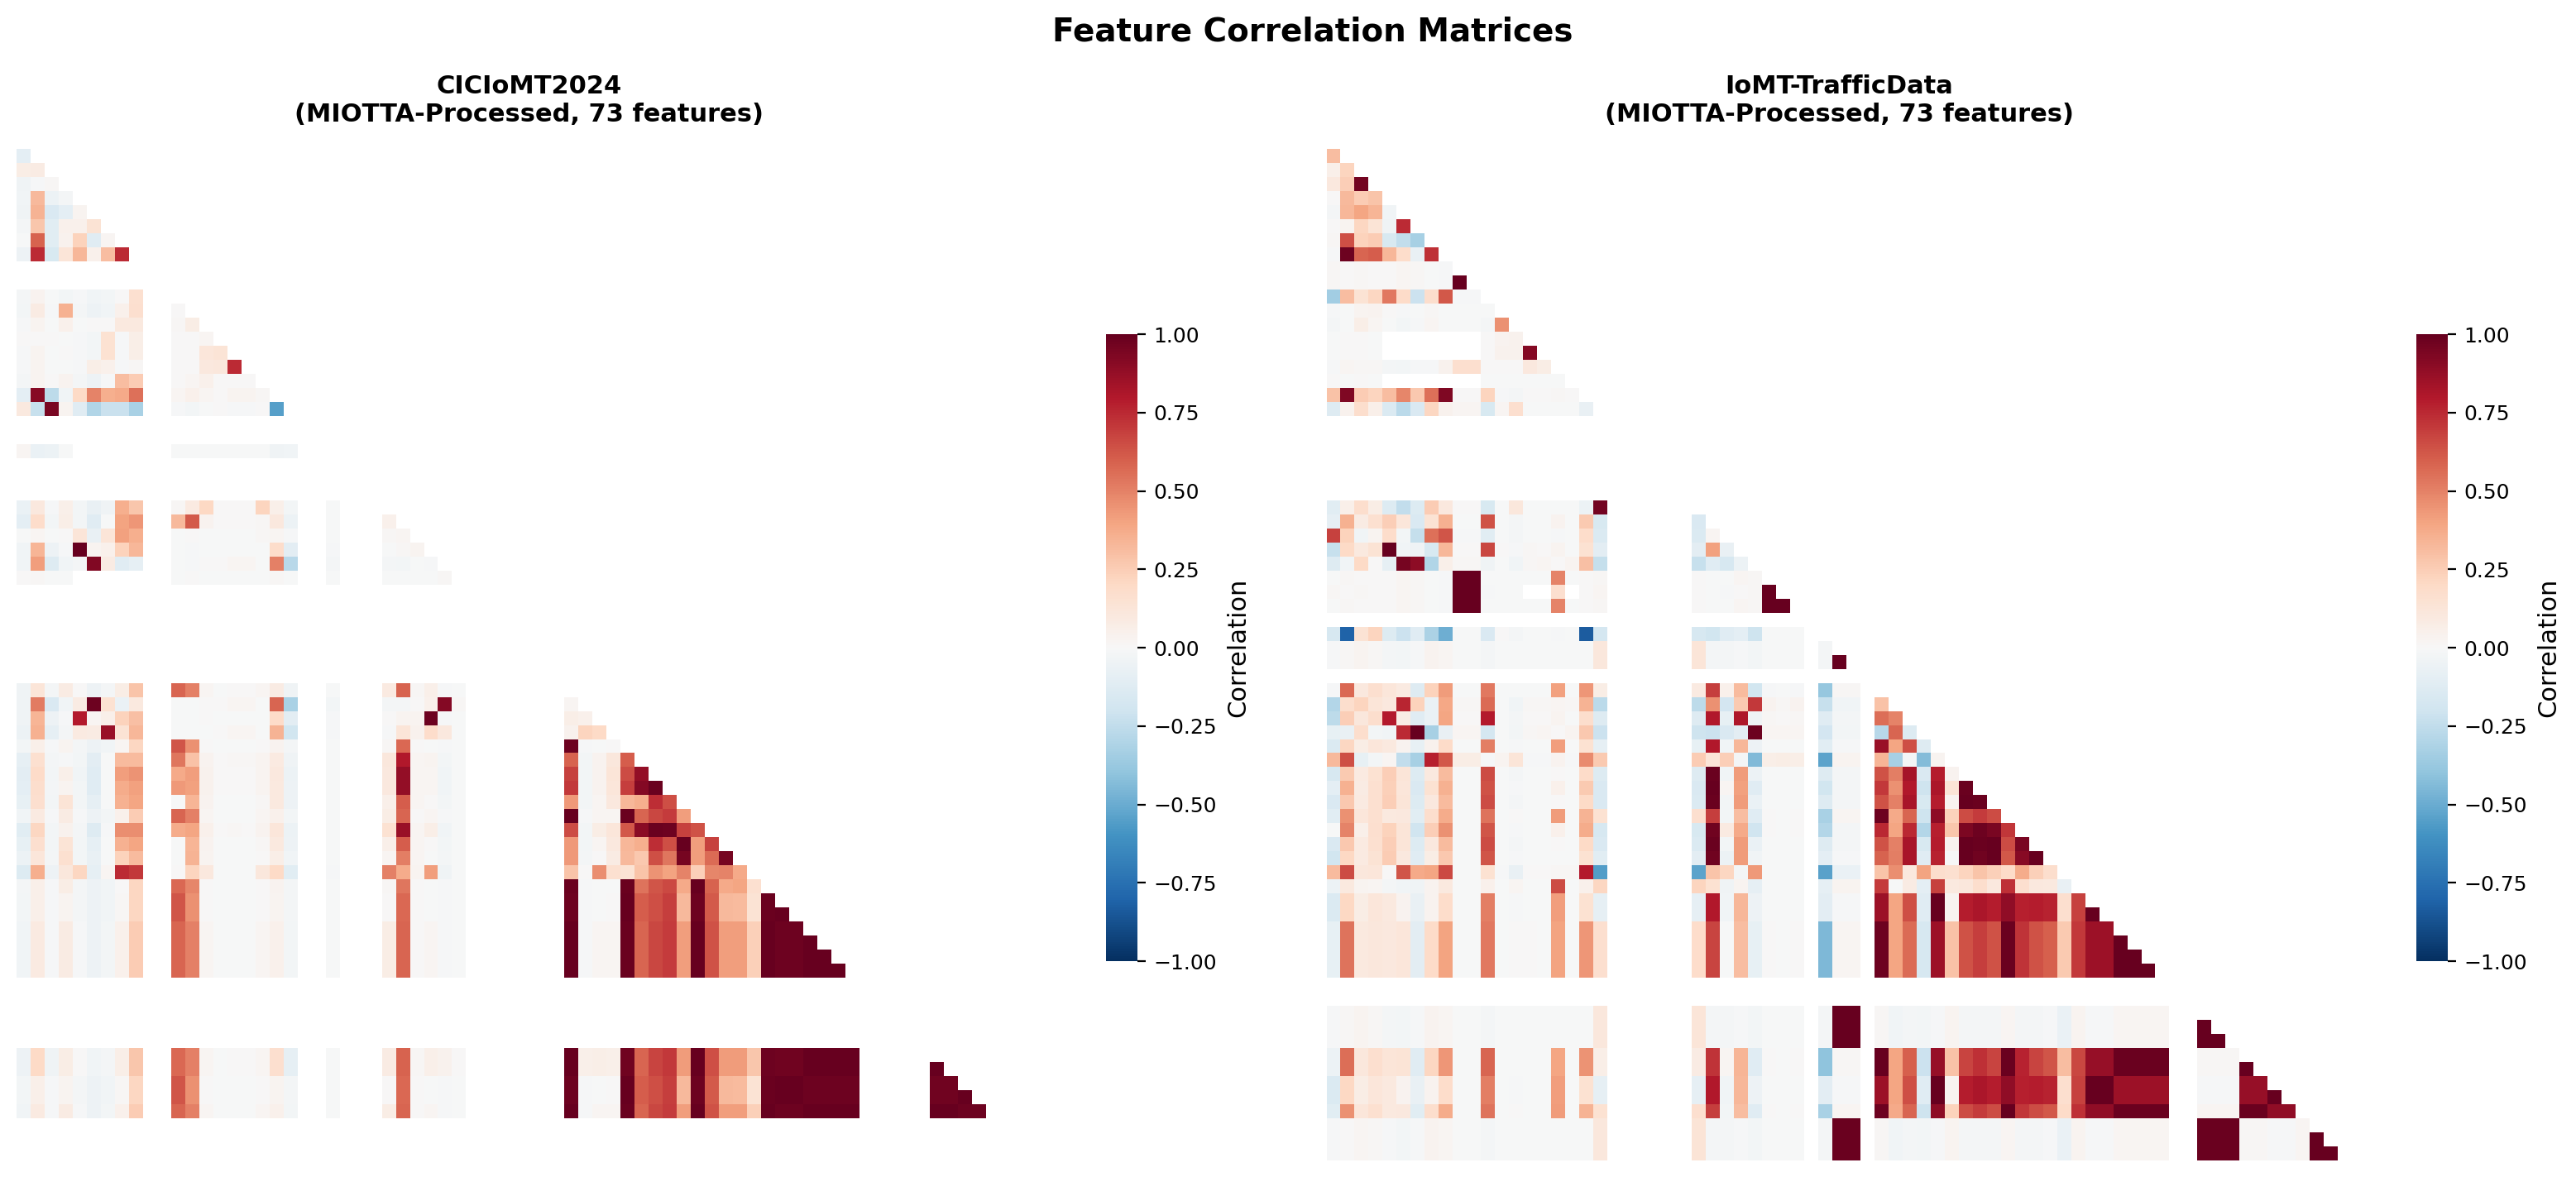
\includegraphics[width=\textwidth]{correlation_heatmaps.png}
\caption{Feature correlation matrices for CICIoMT2024 (left) and IoMT-TrafficData (right), both MIOTTA-processed. Similar overall correlation patterns are observed, with clusters of highly correlated features in the packet statistics and TCP flag groups.}
\label{fig:correlation-heatmaps}
\end{figure}

The analysis of missing values, presented in Figure~\ref{fig:missing-values}, reveals that certain features (primarily TCP flag statistics) contain NaN values. This is expected behavior: windows that contain only non-TCP traffic (e.g., purely ARP or UDP traffic) naturally lack TCP flag statistics. The integration pipeline addresses this through targeted imputation with zero values for protocol-absent features.

\begin{figure}[htbp]
\centering
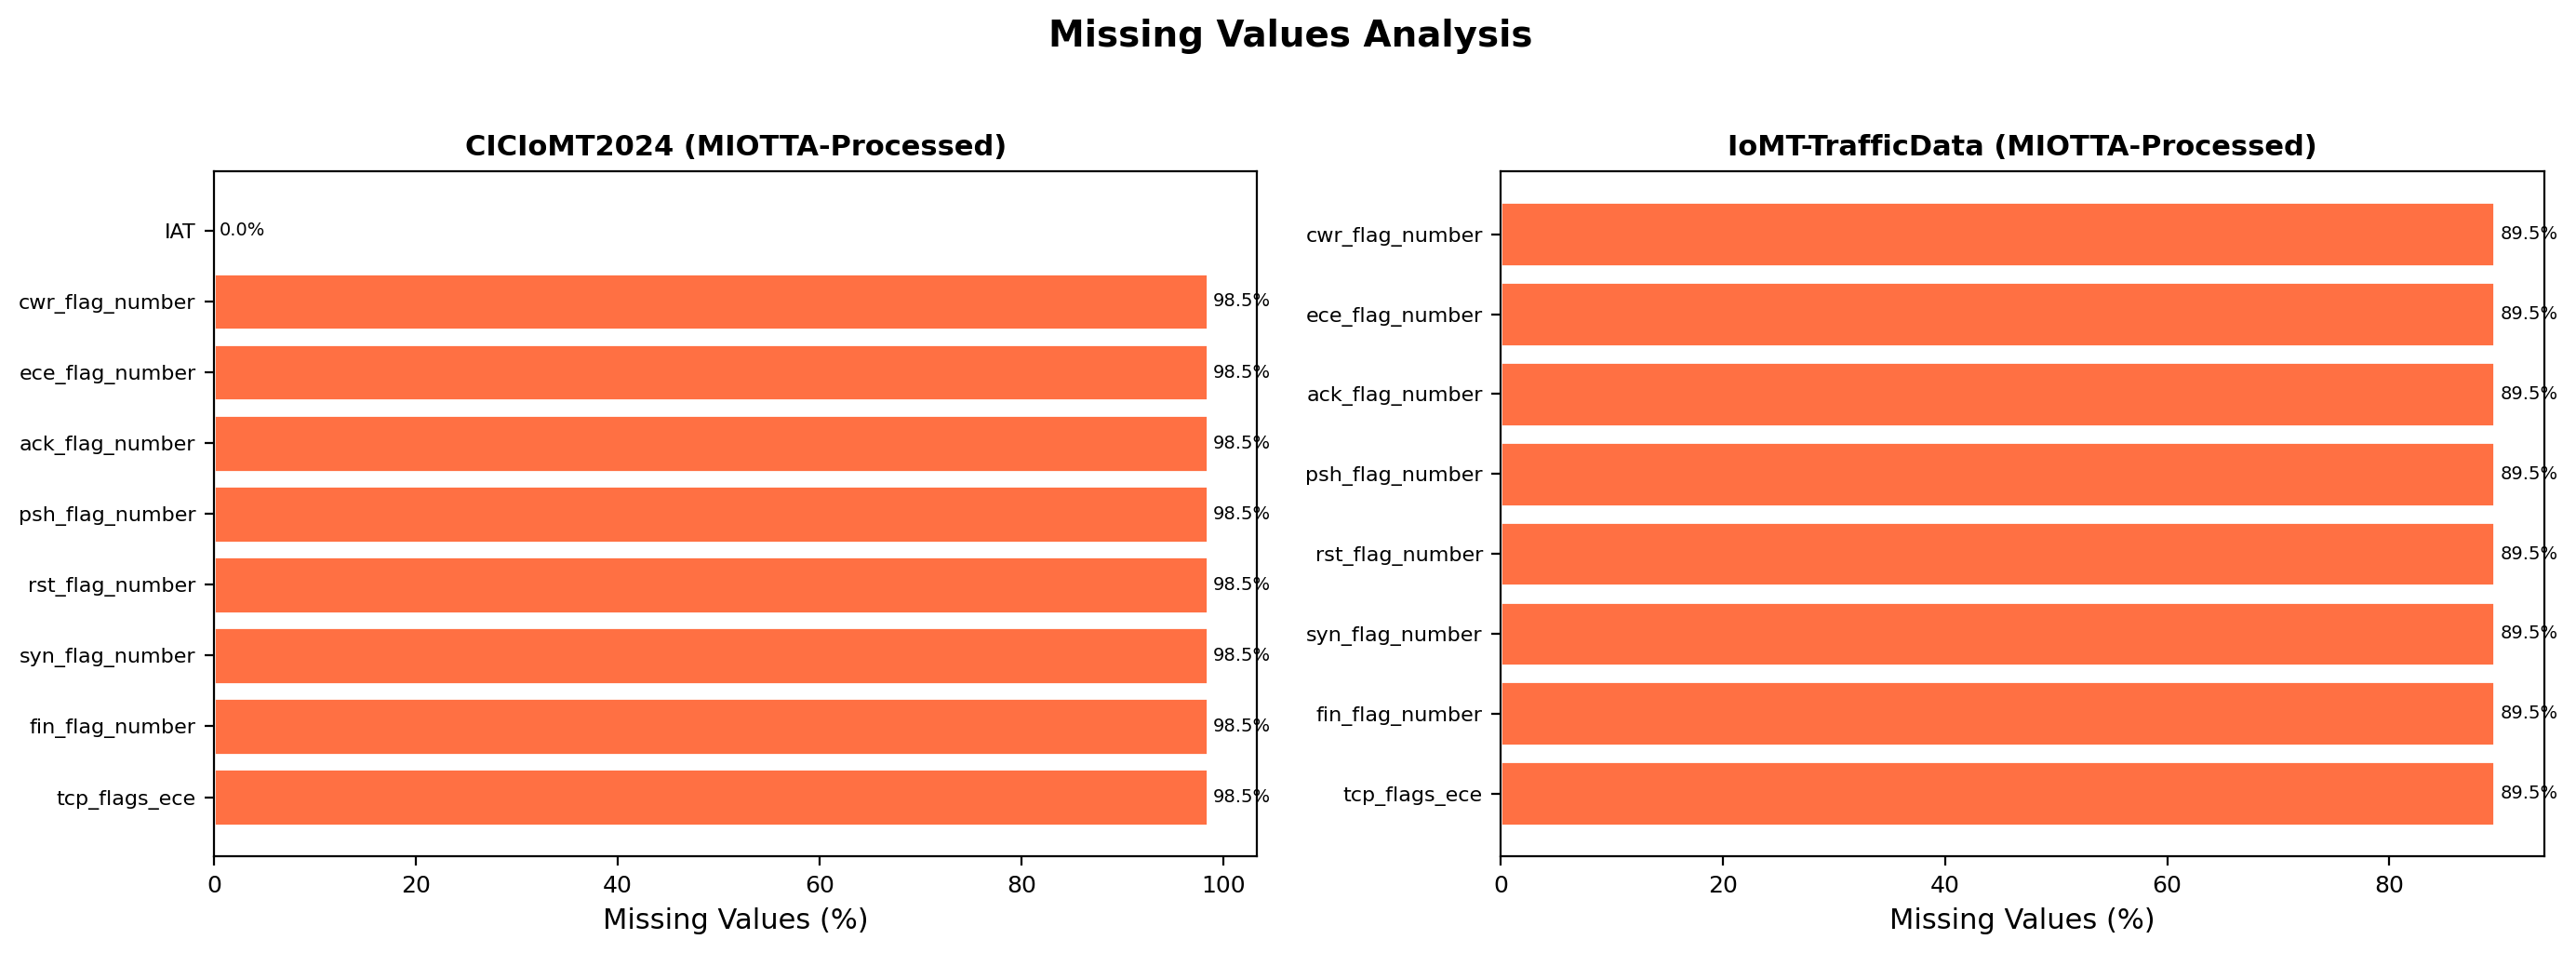
\includegraphics[width=\textwidth]{missing_values_analysis.png}
\caption{Missing values analysis for both MIOTTA-processed datasets. NaN values are concentrated in TCP flag features and arise from windows containing only non-TCP traffic---an expected and well-understood pattern.}
\label{fig:missing-values}
\end{figure}

\subsection{CICIoT2023 --- Planned MIOTTA Processing}
\label{subsec:miotta-ciciot-planned}

The CICIoT2023 dataset will be processed through MIOTTA-NPT using the same configuration (combined mode, window size of 100 packets) as part of Phase~2. Based on the verified behavior of the tool with the first two datasets, the processing is expected to yield the same 73-feature space, enabling seamless concatenation with the Phase~1 unified dataset.

\clearpage
\begin{figure}[p]
\centering
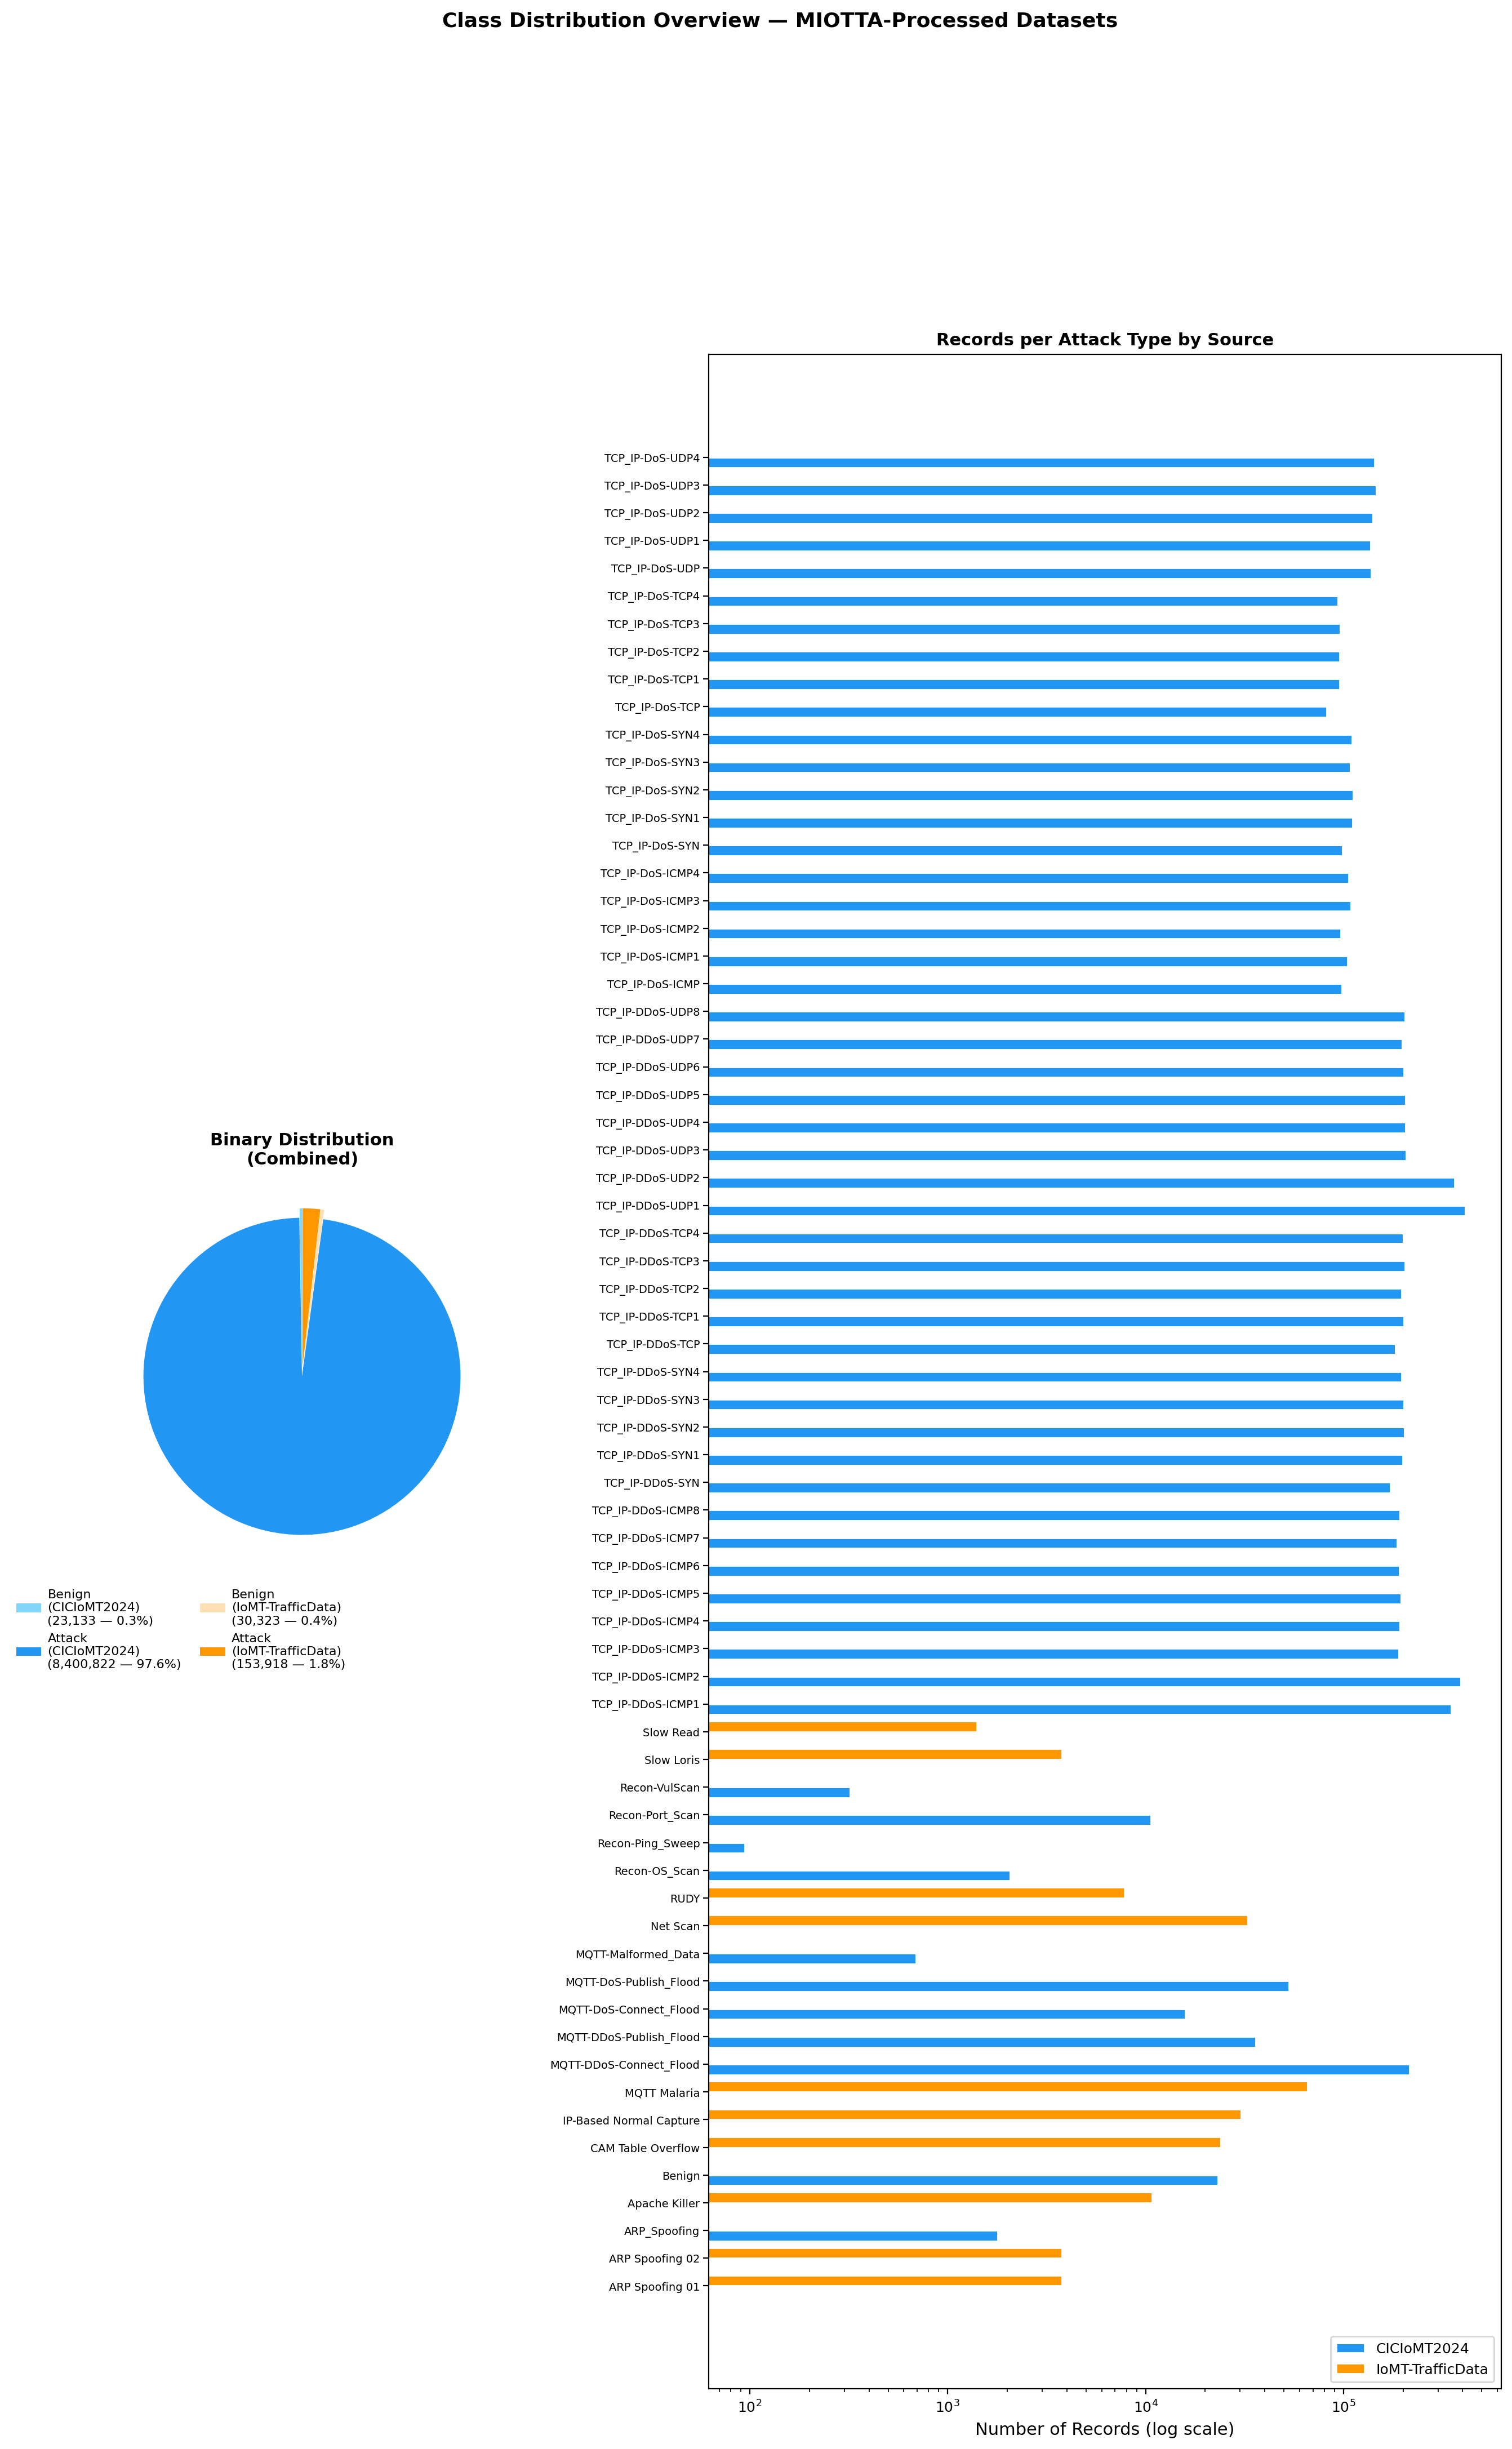
\includegraphics[height=0.85\textheight, keepaspectratio]{combined_class_distribution.png}
\caption{Class distribution overview of the two MIOTTA-processed datasets. Left: binary (benign vs. attack) composition showing the relative contribution of each dataset. Right: per-attack-type record counts by source dataset (logarithmic scale), illustrating the complementary attack coverage.}
\label{fig:combined-class-dist}
\end{figure}
\clearpage

% ══════════════════════════════════════════════════════════════════════════════
\section{Integration Pipeline Execution}
\label{sec:pipeline-execution}

This section documents the step-by-step execution of the integration pipeline, from label harmonization through to the production of the final unified dataset. Figure~\ref{fig:combined-class-dist} provides an overview of the class composition across the two datasets prior to integration.

\subsection{Label Harmonization Implementation}
\label{subsec:label-implementation}

The label harmonization stage applies the three-level labeling scheme defined in Section~\ref{sec:label-harmonization} through explicit mapping dictionaries maintained as configuration artifacts. Each original attack label is deterministically mapped to three harmonized levels: binary (\texttt{label\_binary}), category (\texttt{label\_category}), and fine-grained (\texttt{label\_fine}).

\paragraph{CICIoMT2024 Mapping.}
The CICIoMT2024 dataset contains 18 distinct attack types plus benign traffic. Table~\ref{tab:ciciomt-mapping} presents the complete mapping used in the final Phase~1 dataset. Attack labels are inferred from the MIOTTA output filenames and normalized by stripping numeric suffixes (e.g., \texttt{TCP\_IP-DDoS-ICMP1} through \texttt{TCP\_IP-DDoS-ICMP8} are collapsed to \texttt{TCP\_IP-DDoS-ICMP}). In this operational mapping, all MQTT-related attacks are grouped under the dedicated \texttt{MQTT} category to preserve protocol semantics for downstream model training and evaluation.

\begin{table}[htbp]
\centering
\caption{CICIoMT2024 label harmonization mapping used in Phase~1. The 19 original labels (including Benign) are mapped to 6 categories, including dedicated \texttt{MQTT}.}
\label{tab:ciciomt-mapping}
\small
\begin{tabularx}{\textwidth}{@{}l l l@{}}
\toprule
\textbf{Original Label (label\_fine)} & \textbf{Category} & \textbf{Binary} \\
\midrule
Benign & Benign & Benign \\
\addlinespace
TCP\_IP-DDoS-ICMP & DDoS & Attack \\
TCP\_IP-DDoS-UDP & DDoS & Attack \\
TCP\_IP-DDoS-SYN & DDoS & Attack \\
TCP\_IP-DDoS-TCP & DDoS & Attack \\
MQTT-DDoS-Connect\_Flood & MQTT & Attack \\
MQTT-DDoS-Publish\_Flood & MQTT & Attack \\
\addlinespace
TCP\_IP-DoS-UDP & DoS & Attack \\
TCP\_IP-DoS-SYN & DoS & Attack \\
TCP\_IP-DoS-ICMP & DoS & Attack \\
TCP\_IP-DoS-TCP & DoS & Attack \\
MQTT-DoS-Connect\_Flood & MQTT & Attack \\
MQTT-DoS-Publish\_Flood & MQTT & Attack \\
\addlinespace
Recon-Port\_Scan & Reconnaissance & Attack \\
Recon-OS\_Scan & Reconnaissance & Attack \\
Recon-VulScan & Reconnaissance & Attack \\
Recon-Ping\_Sweep & Reconnaissance & Attack \\
\addlinespace
ARP\_Spoofing & Spoofing & Attack \\
\addlinespace
MQTT-Malformed\_Data & MQTT & Attack \\
\bottomrule
\end{tabularx}
\end{table}

\paragraph{IoMT-TrafficData Mapping.}
The IoMT-TrafficData dataset uses descriptive filenames as attack labels. Table~\ref{tab:iomt-mapping} presents the mapping. Notably, two ARP Spoofing captures (variants 01 and 02) are consolidated into a single fine-grained label \texttt{ARP\_Spoofing}. In the dedicated MQTT mapping, \texttt{MQTT Malaria} is assigned to \texttt{MQTT}, while the remaining service-availability attacks (Apache Killer, CAM Table Overflow, SlowLoris, SlowRead, RUDY) remain in \texttt{DoS}.

\begin{table}[htbp]
\centering
\caption{IoMT-TrafficData label harmonization mapping used in Phase~1. The 10 original labels are mapped to 5 categories, including dedicated \texttt{MQTT}.}
\label{tab:iomt-mapping}
\small
\begin{tabularx}{\textwidth}{@{}l l l l@{}}
\toprule
\textbf{Original Label} & \textbf{Fine-Grained} & \textbf{Category} & \textbf{Binary} \\
\midrule
IP-Based Normal Capture & Benign & Benign & Benign \\
\addlinespace
MQTT Malaria & MQTT\_Malaria & MQTT & Attack \\
CAM Table Overflow & CAM\_Table\_Overflow & DoS & Attack \\
Apache Killer & Apache\_Killer & DoS & Attack \\
RUDY & RUDY & DoS & Attack \\
Slow Loris & SlowLoris & DoS & Attack \\
Slow Read & SlowRead & DoS & Attack \\
\addlinespace
Net Scan & Net\_Scan & Reconnaissance & Attack \\
\addlinespace
ARP Spoofing 01 & ARP\_Spoofing & Spoofing & Attack \\
ARP Spoofing 02 & ARP\_Spoofing & Spoofing & Attack \\
\bottomrule
\end{tabularx}
\end{table}

After harmonization, CICIoMT2024 spans 6 categories (DDoS, DoS, MQTT, Benign, Reconnaissance, Spoofing), while IoMT-TrafficData spans 5 categories (DoS, MQTT, Reconnaissance, Benign, Spoofing). The validation step confirmed that every original label was successfully mapped---no unmapped labels remained.

\subsection{Data Quality Treatment}
\label{subsec:quality-treatment}

The data quality assurance pipeline was applied to the unified dataset (8,608,196 rows, 73 features) in six sequential steps, as specified in Section~\ref{sec:quality}. Figure~\ref{fig:qa-impact} summarizes the aggregate impact.

\begin{figure}[htbp]
\centering
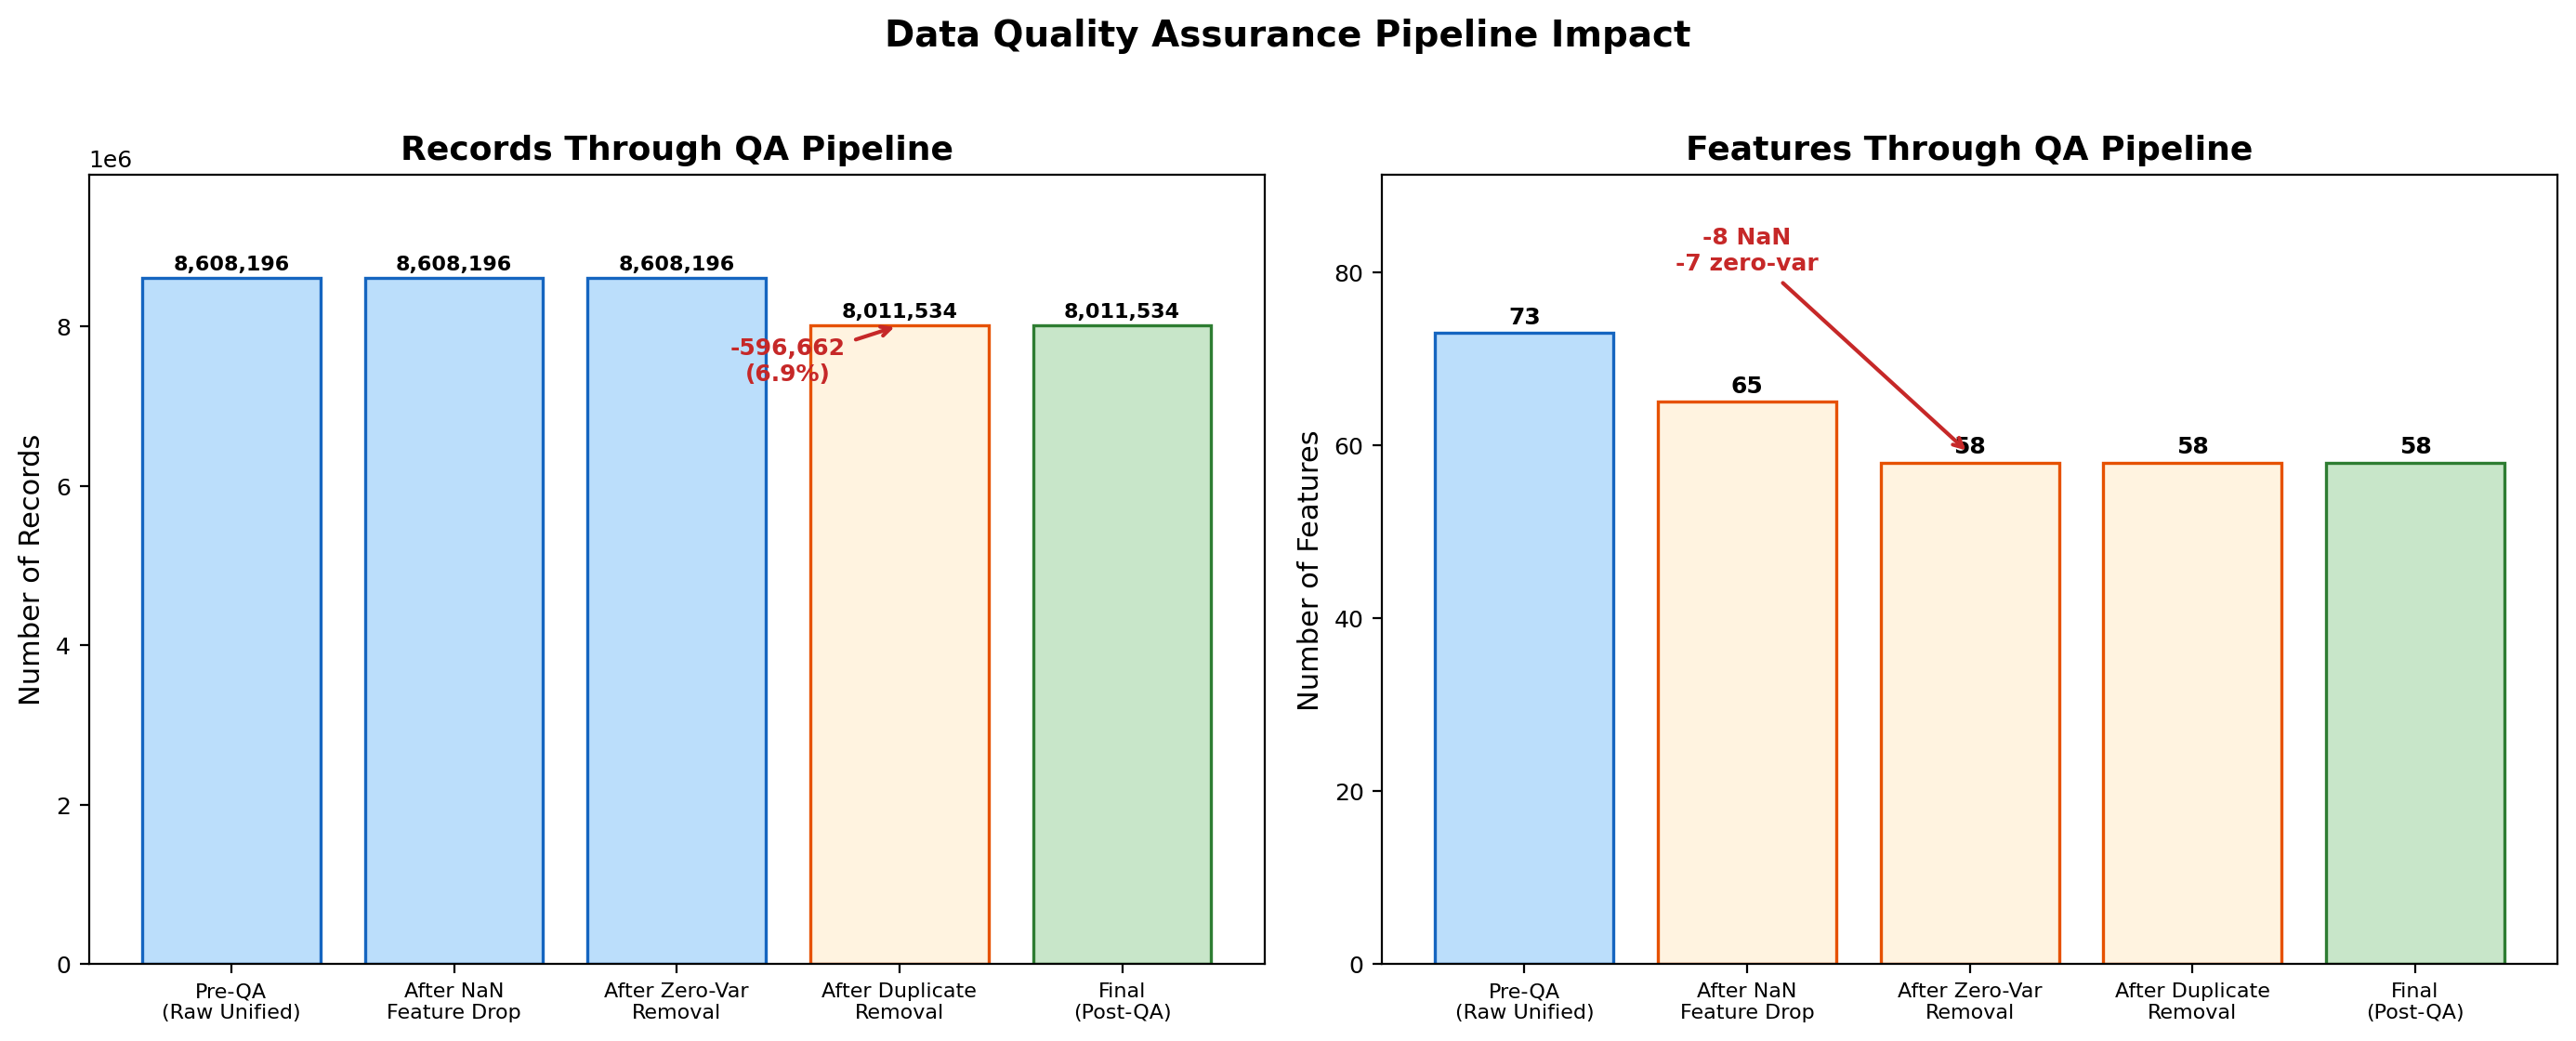
\includegraphics[width=\textwidth]{qa_impact_summary.png}
\caption{Impact of the data quality assurance pipeline on dataset dimensions. Left: record count reduction through duplicate removal. Right: feature reduction through high-NaN and zero-variance feature elimination.}
\label{fig:qa-impact}
\end{figure}

\paragraph{Step 1 --- Missing Value Treatment.}
Features with a NaN rate exceeding the 50\% threshold were dropped entirely. Eight TCP flag statistics met this criterion---\texttt{fin\_flag\_number}, \texttt{syn\_flag\_number}, \texttt{rst\_flag\_number}, \texttt{psh\_flag\_number}, \texttt{ack\_flag\_number}, \texttt{ece\_flag\_number}, \texttt{cwr\_flag\_number}, and \texttt{tcp\_flags\_ece}---all exhibiting 98.28\% missingness. This extreme rate is explained by the MIOTTA-NPT processing: these features count per-flag occurrences within a window, but when the window contains exclusively non-TCP traffic (UDP, ICMP, or ARP), no TCP flags exist and the values are recorded as NaN. Since 98.28\% of windows across both datasets lack these values, the features carry negligible discriminative information and their removal is justified. After dropping these 8 features, exactly 1 residual NaN value remained across the entire dataset, which was imputed with 0 following the protocol-absence pattern.

\paragraph{Step 2 --- Infinity Value Handling.}
A scan for $\pm\infty$ values found \textbf{zero infinity values} in any of the remaining 65 features. This indicates that the MIOTTA-NPT extraction tool handles edge cases (e.g., division by zero in rate computations) gracefully, producing NaN rather than infinity.

\paragraph{Step 3 --- Zero-Variance Feature Removal.}
Seven features exhibited exactly zero variance across the entire unified dataset and were removed: \texttt{DHCP}, \texttt{ARP}, \texttt{IPV4}, \texttt{LLC}, \texttt{Drate}, \texttt{Fwd\_Data\_Pkts\_Tot}, and \texttt{Bwd\_Data\_Pkts\_Tot}. These constant-valued features carry no discriminative information for classification. Their presence reflects either protocol indicators that never trigger in the IoMT traffic or aggregation counters that are always zero in the combined mode.

\paragraph{Step 4 --- Near-Zero-Variance Detection.}
Four additional features were flagged as having near-zero variance (below $10^{-8}$): \texttt{IGMP}, \texttt{Fwd\_IAT}, \texttt{Bwd\_IAT}, and \texttt{Flow\_IAT}. These were \textit{not} removed, as they may still carry useful information for specific attack categories, but they were recorded in the pipeline metadata for consideration during model evaluation.

\paragraph{Step 5 --- Duplicate Removal.}
Exact duplicate detection, applied on feature columns only (excluding metadata and label columns), identified and removed \textbf{596,662 duplicate rows} (6.93\% of the pre-QA dataset). Duplicates arise from the window-based aggregation methodology: consecutive windows of identical packet patterns produce identical feature vectors, particularly common in DDoS flood attacks where sustained high-volume traffic creates highly repetitive patterns. The first occurrence of each unique row was retained.

\paragraph{Step 6 --- Type Consistency.}
All 58 remaining feature columns were cast from their original \texttt{float64} type to \texttt{float32}, halving memory requirements while preserving sufficient numerical precision for ML training. This standardization ensures that all features use a uniform data type regardless of their source dataset.

\subsection{Dataset Concatenation and Source Attribution}
\label{subsec:concatenation}

Prior to quality assurance, the two harmonized datasets were concatenated into a single unified DataFrame. The concatenation was performed using a simple vertical stack (\texttt{pd.concat}), made possible by the identical feature schema guaranteed by MIOTTA-NPT processing.

Each record retains three provenance columns: \texttt{source\_dataset} identifies the originating dataset (\texttt{CICIoMT2024} or \texttt{IoMT-TrafficData}), \texttt{source\_file} records the specific MIOTTA output CSV file, and \texttt{attack\_type} preserves the original label as inferred from the filename. These columns enable cross-domain evaluation and per-source performance disaggregation, as discussed in Section~\ref{sec:provenance}.

The pre-QA unified dataset comprised 8,608,196 records (8,423,955 from CICIoMT2024, representing 97.86\%, and 184,241 from IoMT-TrafficData, representing 2.14\%) with 73 features and 7 metadata/label columns (80 columns total). After the complete QA pipeline, the final unified dataset contains \textbf{8,011,534 records} across \textbf{58 features}, plus the label and metadata columns.

\subsection{Feature Scaling}
\label{subsec:scaling-execution}

Feature scaling was applied using \textbf{standardization} ($z$-score normalization), transforming each feature to zero mean and unit variance. To prevent data leakage, the scaling parameters (per-feature mean and standard deviation) were computed exclusively on the training partition and then applied identically to the validation and test partitions.

The implementation uses scikit-learn's \texttt{StandardScaler}, fitted on the training set's 58 feature columns. Post-scaling verification confirmed that the training set achieves a mean $\approx 0.000000$ and standard deviation $\approx 1.000000$ across all features, as expected. The validation and test sets exhibit means and standard deviations very close to---but not exactly---0 and 1, which is the correct behavior: slight deviations confirm that no information from these partitions leaked into the scaling parameters.

The fitted scaler object is persisted as a \texttt{joblib} artifact (\texttt{scaler.joblib}), enabling its reuse during model inference to ensure that new data undergoes identical preprocessing.

\subsection{Stratified Splitting}
\label{subsec:splitting-execution}

The unified dataset was partitioned into training, validation, and test sets using scikit-learn's \texttt{train\_test\_split} with stratification on the composite key \texttt{label\_category} $\times$ \texttt{source\_dataset}. This dual stratification ensures that both the attack category distribution and the source dataset proportions are preserved in each partition, preventing any partition from accidentally excluding rare attack types or under-representing a source dataset.

The split was performed in two stages: first, 70\% of the data was allocated to the training set and 30\% to a temporary hold-out; then, the hold-out was divided equally into 15\% validation and 15\% test. Table~\ref{tab:split-sizes} presents the resulting partition sizes.

\begin{table}[htbp]
\centering
\caption{Stratified split sizes for the Phase~1 unified dataset.}
\label{tab:split-sizes}
\small
\begin{tabular}{@{}l r r r r@{}}
\toprule
\textbf{Partition} & \textbf{Records} & \textbf{\%} & \textbf{CICIoMT2024} & \textbf{IoMT-TrafficData} \\
\midrule
Train & 5,608,073 & 70.0\% & 5,479,105 (97.70\%) & 128,968 (2.30\%) \\
Validation & 1,201,730 & 15.0\% & 1,174,094 (97.70\%) & 27,636 (2.30\%) \\
Test & 1,201,731 & 15.0\% & 1,174,094 (97.70\%) & 27,637 (2.30\%) \\
\midrule
\textbf{Total} & \textbf{8,011,534} & \textbf{100\%} & \textbf{7,827,293} & \textbf{184,241} \\
\bottomrule
\end{tabular}
\end{table}

Figure~\ref{fig:split-verification} confirms that stratification successfully preserves both category and source proportions across all three partitions for the dedicated MQTT mapping. Category proportions remain near-identical across train/validation/test (DDoS: 67.01\%, DoS: 26.82\%, MQTT: 4.82\%, Benign: 0.67\%, Reconnaissance: 0.57\%, Spoofing: 0.12\%), while source proportions are preserved to within $\pm0.01\%$. This level of consistency is essential for ensuring that model evaluation metrics are not confounded by partition-level distribution differences.

\begin{figure}[htbp]
\centering
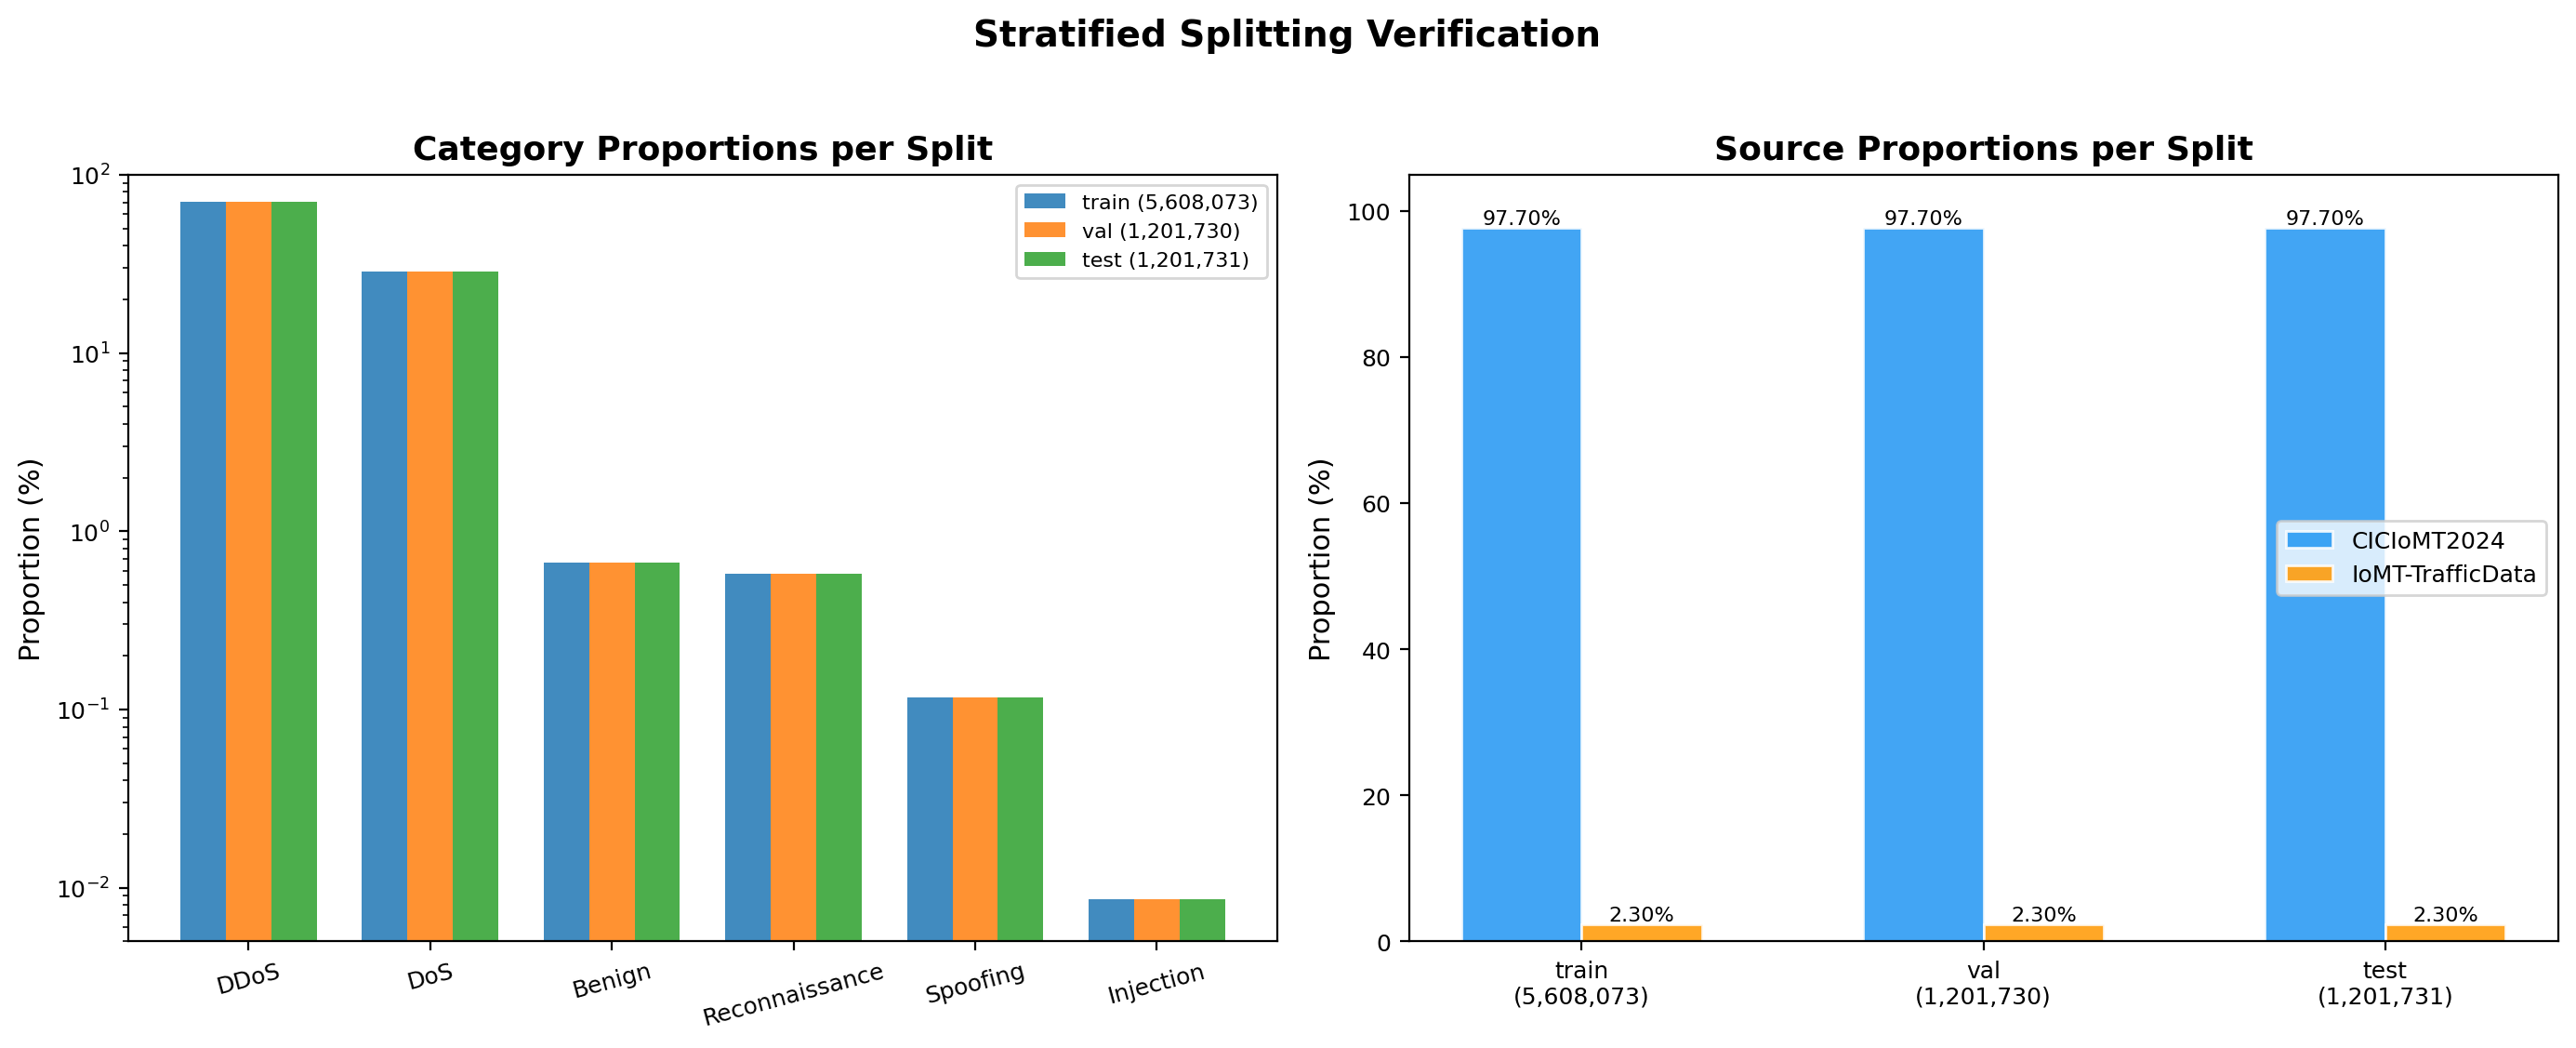
\includegraphics[width=\textwidth]{split_verification.png}
\caption{Verification of stratified splitting. Left: category proportions per partition (logarithmic scale). Right: source dataset proportions per partition. The near-identical proportions confirm successful stratification.}
\label{fig:split-verification}
\end{figure}

% ══════════════════════════════════════════════════════════════════════════════
\section{Unified Dataset Description}
\label{sec:unified-description}

The Phase~1 integration pipeline produces a unified IoMT intrusion detection dataset that combines traffic from two complementary IoMT environments into an ML-ready resource. Following supervisor guidance, all subsequent experiments in this thesis adopt the dedicated MQTT category mapping at Level-2, where all MQTT-related attacks are grouped under \texttt{MQTT}. This section characterizes the final dataset used for model development.

\subsection{Dataset Overview}
\label{subsec:dataset-overview}

The final unified dataset comprises \textbf{8,011,534 records} described by \textbf{58 numeric features}, partitioned into training (5,608,073), validation (1,201,730), and test (1,201,731) sets. All features are standardized with \texttt{StandardScaler} using train-only fitting (fit on train; transform on train/validation/test), cast to \texttt{float32} for memory efficiency, and verified to contain no missing, infinite, or constant-valued entries.

\subsection{Label Distributions}
\label{subsec:label-distributions}

The three-level labeling scheme provides classification targets at different granularities:

\begin{itemize}
    \item \textbf{Binary level}: 99.33\% of records are labeled as \texttt{Attack} and 0.67\% as \texttt{Benign}, reflecting the attack-heavy nature of the source datasets.

    \item \textbf{Category level}: Six categories are present, with the distribution shown in Figure~\ref{fig:unified-categories}. DDoS dominates with 67.01\% of records, followed by DoS (26.82\%), MQTT (4.82\%), Benign (0.67\%), Reconnaissance (0.57\%), and Spoofing (0.12\%). The maximum-to-minimum ratio is approximately 575:1 (DDoS vs.\ Spoofing), indicating substantial class imbalance that must be addressed during model training.

    \item \textbf{Fine-grained level}: 26 distinct attack types are present, spanning both datasets. The four most common types---\texttt{TCP\_IP-DDoS-ICMP} (21.71\%), \texttt{TCP\_IP-DDoS-UDP} (21.45\%), \texttt{TCP\_IP-DDoS-SYN} (12.09\%), and \texttt{TCP\_IP-DDoS-TCP} (11.76\%)---together account for 67\% of all records. The rarest types, \texttt{Recon-Ping\_Sweep} (94 records) and \texttt{Recon-VulScan} (322 records), constitute less than 0.005\% of the dataset.
\end{itemize}

\begin{figure}[htbp]
\centering
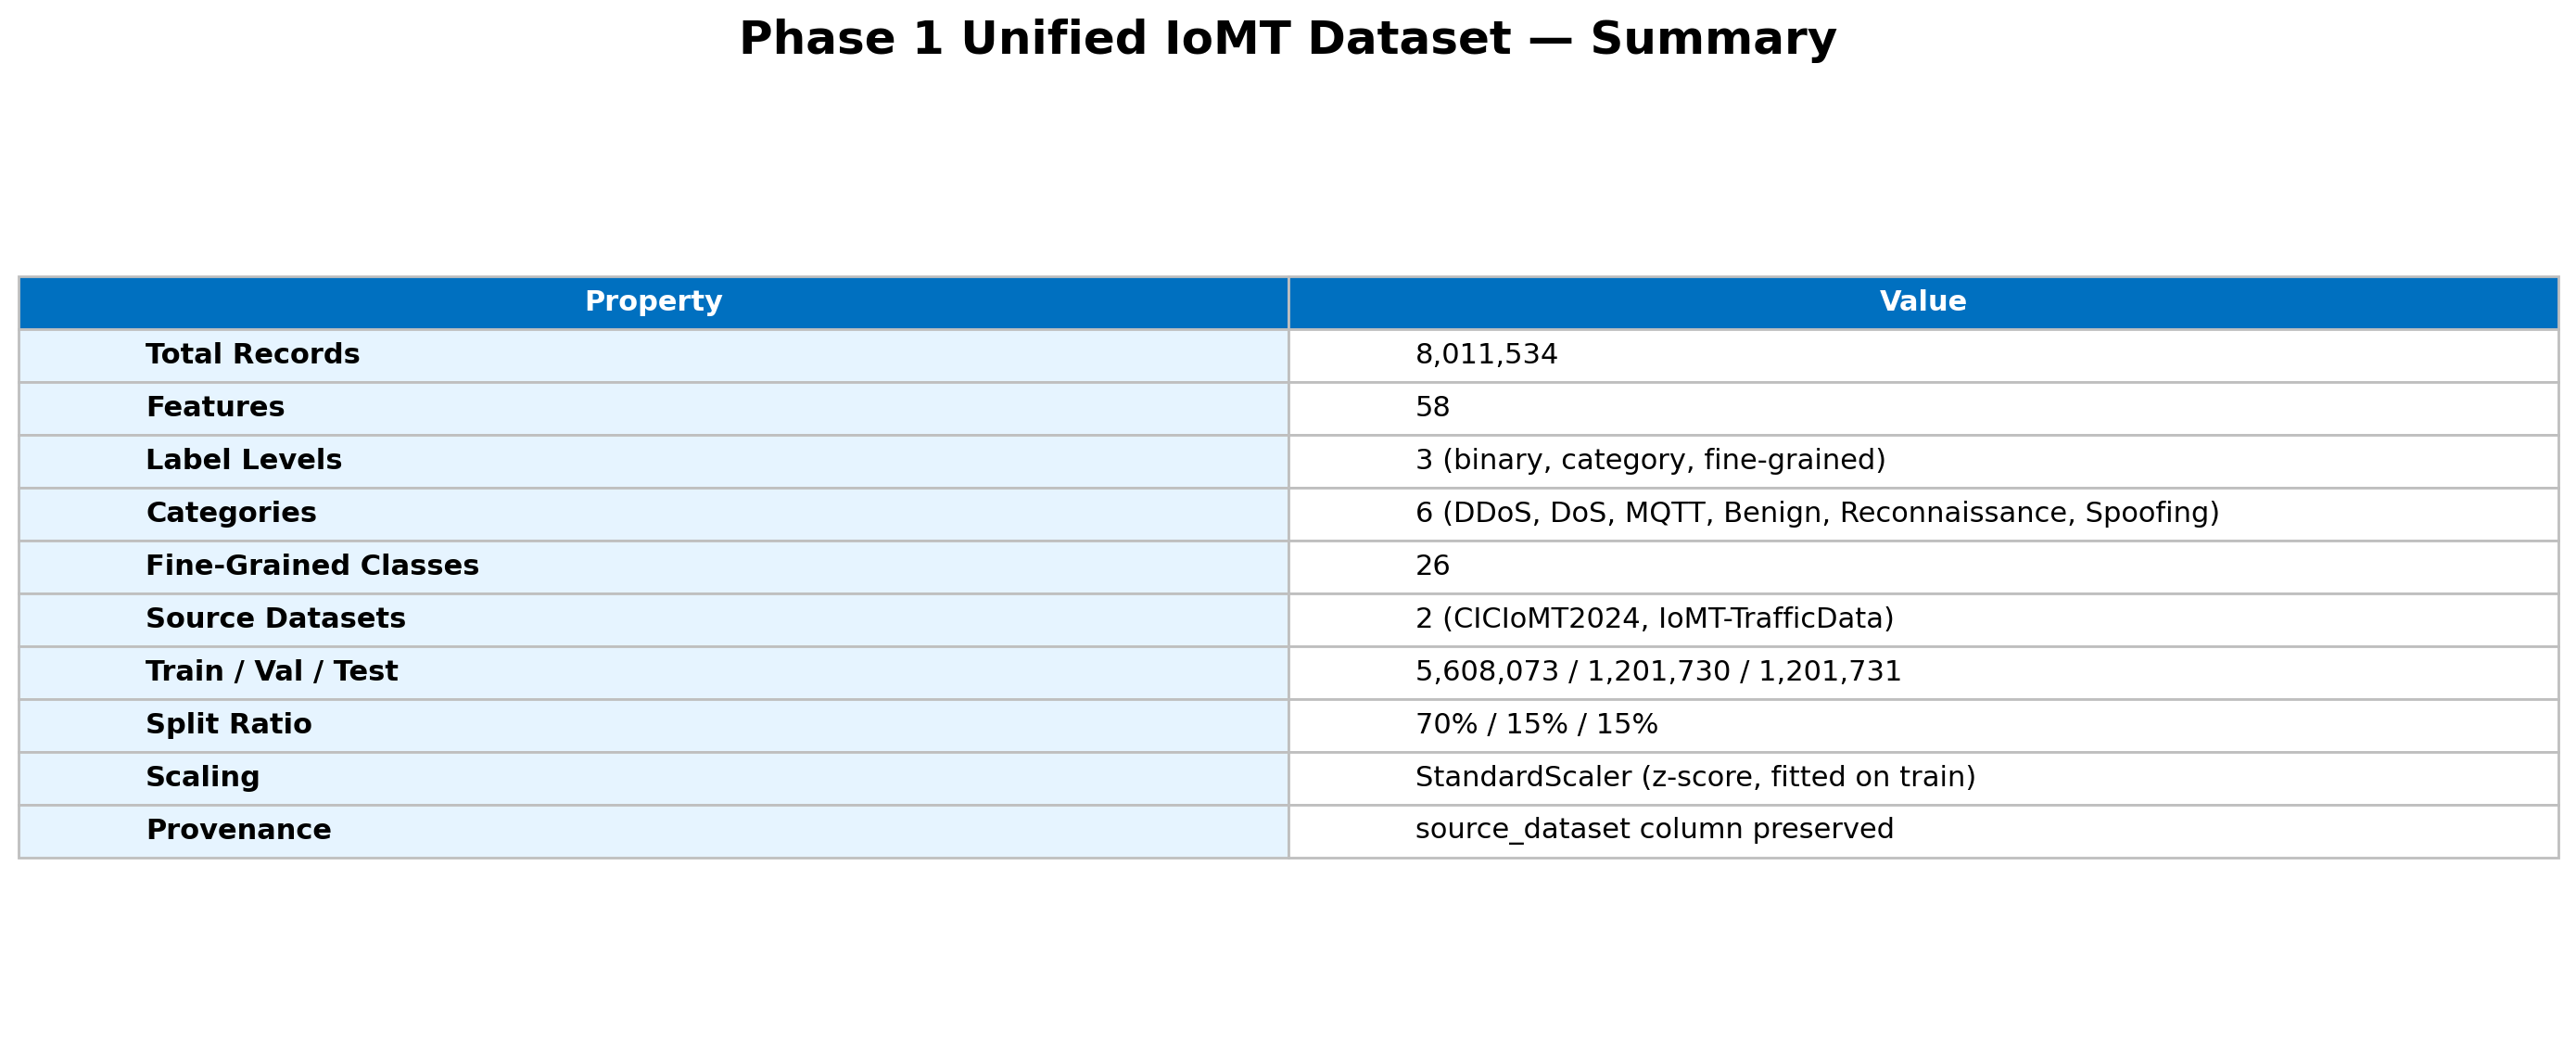
\includegraphics[width=0.85\textwidth]{unified_dataset_summary.png}
\caption{Summary of the final Phase~1 unified IoMT intrusion detection dataset used for model development (dedicated MQTT mapping).}
\label{fig:unified-summary}
\end{figure}

\begin{figure}[htbp]
\centering
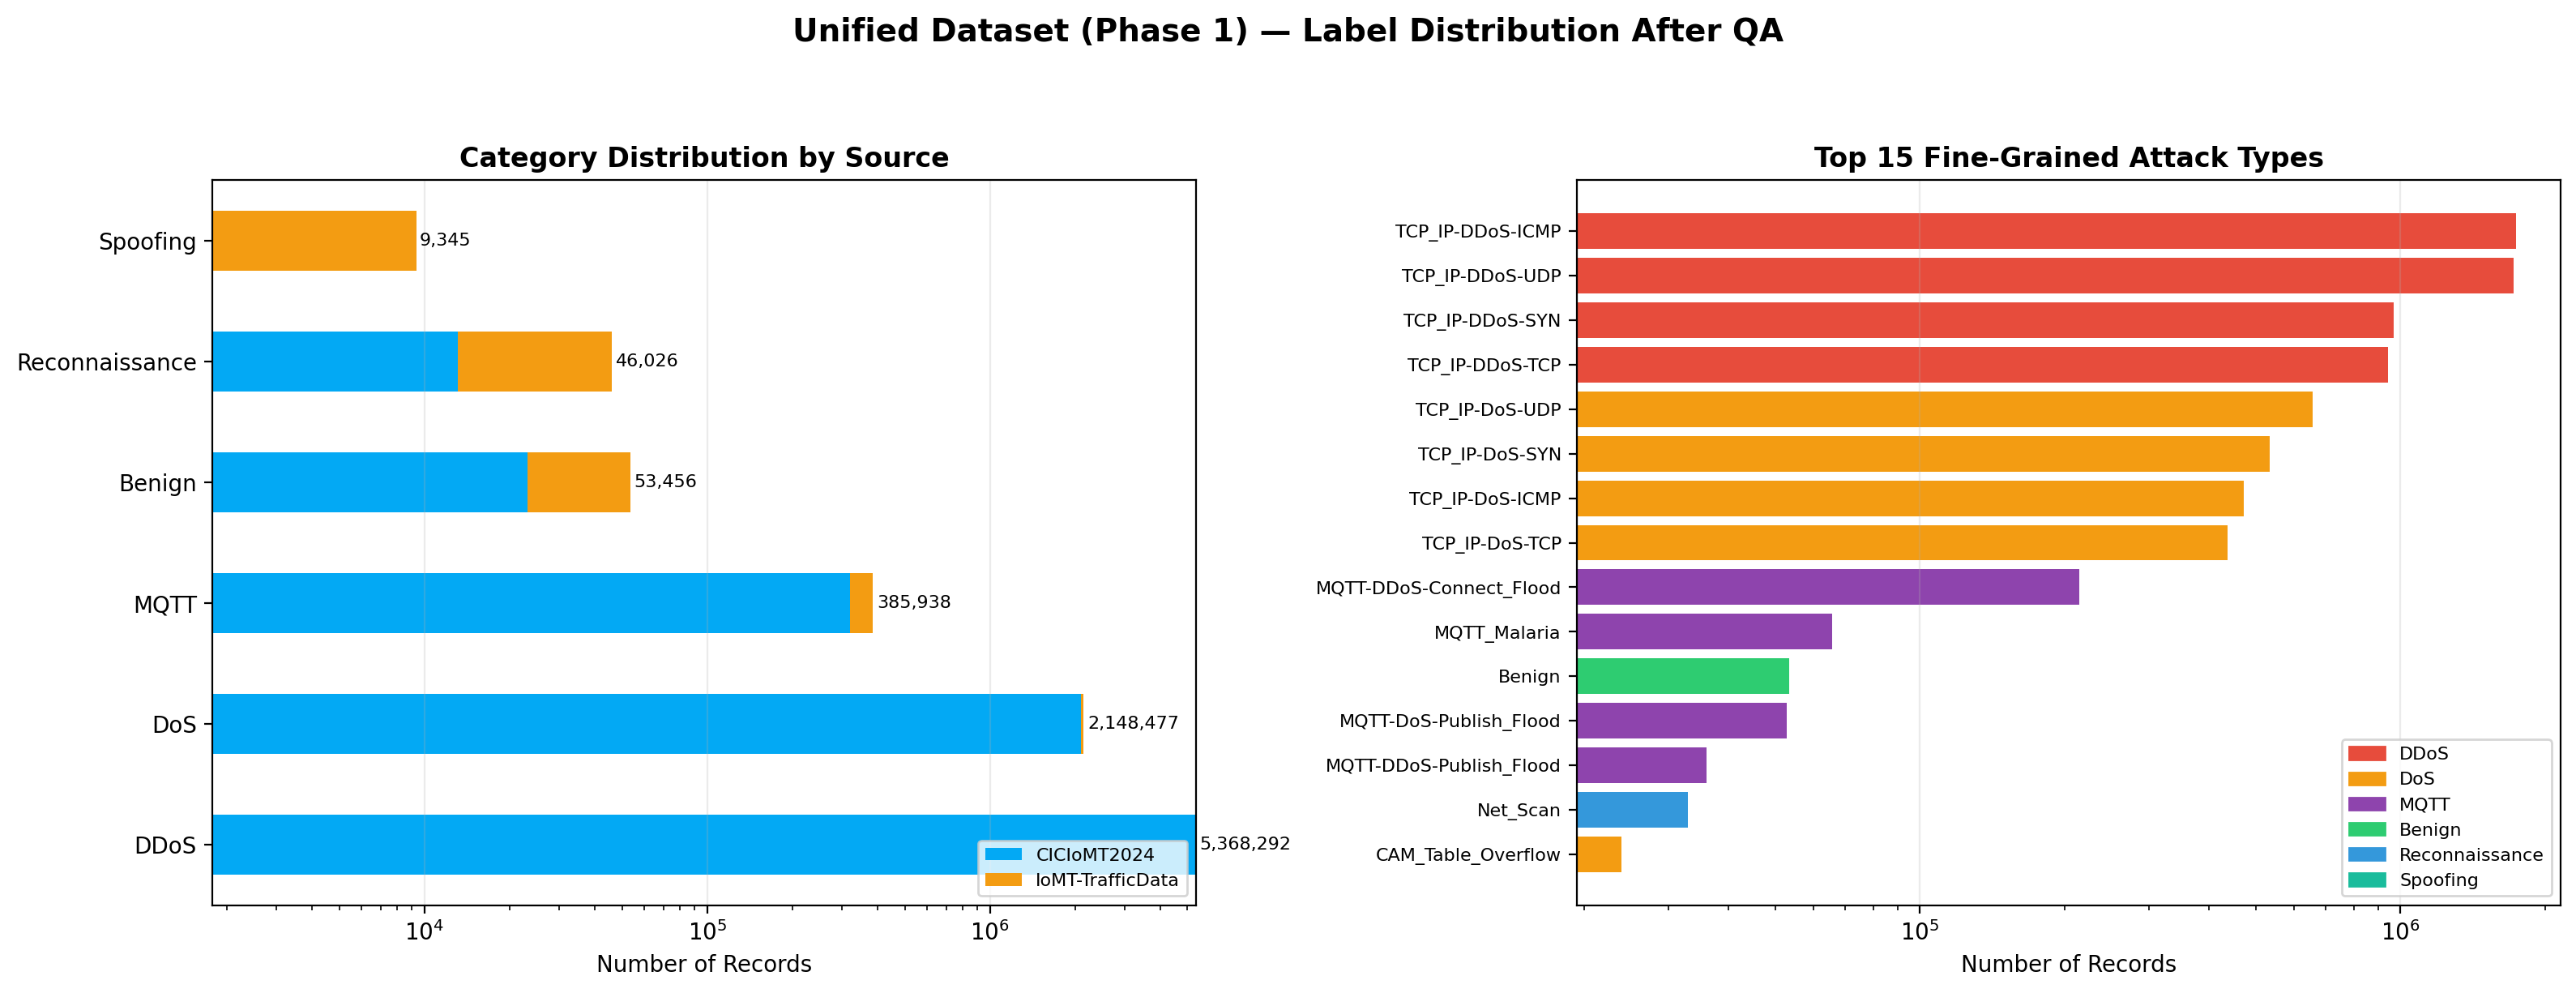
\includegraphics[width=\textwidth]{unified_category_distribution.png}
\caption{Label distribution in the final Phase~1 unified dataset (dedicated MQTT mapping). Left: category-level distribution decomposed by source dataset. Right: the 15 most frequent fine-grained attack types, color-coded by category.}
\label{fig:unified-categories}
\end{figure}

\subsection{Category-Mapping Rationale}
\label{subsec:mqtt-variant}

The dedicated MQTT mapping was selected as the operational taxonomy because the subsequent objective is protocol-aware model evaluation. Concretely, for CICIoMT2024, \texttt{MQTT-DDoS-Connect\_Flood}, \texttt{MQTT-DDoS-Publish\_Flood}, \texttt{MQTT-DoS-Connect\_Flood}, \texttt{MQTT-DoS-Publish\_Flood}, and \texttt{MQTT-Malformed\_Data} are mapped to \texttt{MQTT}; for IoMT-TrafficData, \texttt{MQTT Malaria} is also mapped to \texttt{MQTT}. All other processing stages (quality treatment, stratified splitting, train-only scaler fitting, and export) remain unchanged.

The resulting post-QA category distribution (8,011,534 records, matching the exported CSV splits) is: DDoS 67.01\%, DoS 26.82\%, MQTT 4.82\%, Benign 0.67\%, Reconnaissance 0.57\%, and Spoofing 0.12\%.

\subsection{Cross-Dataset Complementarity}
\label{subsec:complementarity}

A key design objective of the integration was to achieve complementary attack coverage. The unified dataset fulfills this objective: CICIoMT2024 contributes 97.70\% of the records and provides coverage of DDoS, DoS, MQTT, Reconnaissance, and Spoofing categories, while IoMT-TrafficData contributes 2.30\% and introduces 6 unique fine-grained attack types not present in CICIoMT2024---Apache\_Killer, CAM\_Table\_Overflow, MQTT\_Malaria, RUDY, SlowLoris, and SlowRead---covering both \texttt{DoS} and \texttt{MQTT} protocol-oriented behaviors.

Two fine-grained labels appear in both datasets: \texttt{Benign} and \texttt{ARP\_Spoofing}, enabling direct cross-dataset comparison for these specific traffic types. The shared \texttt{ARP\_Spoofing} label (1,782 records from CICIoMT2024, 7,563 from IoMT-TrafficData) is particularly valuable for assessing whether models can generalize the detection of the same attack across different network environments.

\subsection{Storage and Access}
\label{subsec:storage}

The final dataset used in this thesis is stored in \texttt{data/processed/phase1\_iomt\_unified\_mqtt\_category/}, containing the following artifacts:

\begin{itemize}
    \item \texttt{train.csv}, \texttt{val.csv}, \texttt{test.csv}: Scaled data partitions.
    \item \texttt{scaler.joblib}: Fitted \texttt{StandardScaler} object for inference-time preprocessing.
    \item \texttt{metadata.joblib}: Pipeline metadata including the final feature list, near-zero-variance features, and split sizes.
\end{itemize}

The total storage footprint is approximately 6.4~GB in CSV format. Each CSV file contains the 58 scaled features, the three label columns (\texttt{label\_binary}, \texttt{label\_category}, \texttt{label\_fine}), and the provenance columns (\texttt{source\_dataset}, \texttt{source\_file}, \texttt{attack\_type}, \texttt{attack\_group}).

% ══════════════════════════════════════════════════════════════════════════════
\section{Chapter Summary}
\label{sec:execution-summary}

This chapter documented the complete development and execution of the Phase~1 integration pipeline, progressing from exploratory analysis through to the production of unified IoMT intrusion detection datasets. The key contributions and findings of this chapter are:

\begin{enumerate}
    \item \textbf{Exploratory analysis} of three datasets (CICIoMT2024, IoMT-TrafficData, CICIoT2023) revealed fundamental structural incompatibilities in their original feature representations---45, 101, and 47 features respectively, extracted using different tools---confirming the necessity of MIOTTA-NPT for feature standardization.

    \item \textbf{MIOTTA-NPT processing} produced identical 73-feature representations for CICIoMT2024 (8,423,955 records) and IoMT-TrafficData (184,241 records), verified through empirical column-level comparison.

    \item \textbf{Label harmonization} mapped 19 original CICIoMT2024 labels and 10 original IoMT-TrafficData labels into a consistent three-level scheme (binary, category, fine-grained), with dedicated \texttt{MQTT} as the operational Level-2 category space used for all subsequent model development.

    \item \textbf{Data quality assurance} reduced the feature space from 73 to 58 features (removing 8~high-NaN and 7~zero-variance features) and eliminated 596,662 duplicate records (6.93\%), yielding a clean dataset of 8,011,534 records.

    \item \textbf{Stratified splitting} with dual stratification on category and source produced balanced train/validation/test partitions (70/15/15\%) with virtually identical category and source proportions across all three partitions.

    \item \textbf{Feature scaling} using StandardScaler fitted exclusively on the training partition prevents data leakage while ensuring normalized feature ranges for ML model training.
\end{enumerate}

The resulting unified dataset is ready for training and evaluating intrusion detection models in the next stage of this thesis. The pipeline's modular design facilitates extension in Phase~2 to incorporate CICIoT2023, broadening attack coverage to include Mirai botnet, web-based, and brute-force attacks while preserving the same reproducible preprocessing backbone.

\chapter{Experimentation and Evaluation}
\label{ch:experimentation}

This chapter presents the experimental evaluation of the work developed in Chapter~\ref{ch:execution}. The structure follows the logical order of the empirical work: first, assessment of the unified dataset's quality; second, training, comparison, and evaluation of \gls{ids} models on the preprocessed splits (Section~\ref{sec:model-evaluation}); third, synthesis that addresses the research question posed in Section~\ref{sec:rq} in light of those results (Section~\ref{sec:answering-rq}).

% ══════════════════════════════════════════════════════════════════════════════
\section{Unified Dataset Quality Assessment}
\label{sec:quality-assessment}

The quality of the unified dataset is evaluated across multiple dimensions to ensure it meets the requirements for effective \gls{ml} model training.

\subsection{Structural Integrity Verification}
\label{subsec:structural-integrity}

Before proceeding to model training, the exported dataset was subjected to a comprehensive structural integrity audit. The goal is to confirm that the pipeline produced a well-formed, complete, and internally consistent artifact free of residual data-quality issues.

\paragraph{Completeness and absence of defects.}
All 8,011,534 records contain exactly 58 numeric feature columns, with \textbf{zero NaN values} and \textbf{zero infinity values} across the entire feature matrix. Every record has all three label columns (\texttt{label\_binary}, \texttt{label\_category}, \texttt{label\_fine}) and all four provenance columns (\texttt{source\_dataset}, \texttt{source\_file}, \texttt{attack\_type}, \texttt{attack\_group}) fully populated---no missing metadata was found.

\paragraph{Type consistency.}
All 58 feature columns share the same data type (\texttt{float64} after CSV deserialization; \texttt{float32} before export). No mixed-type columns or string-valued features were detected, confirming that the type-casting step in the pipeline operated correctly.

\paragraph{Absence of degenerate features.}
Zero features exhibit constant values across the full dataset, confirming that the zero-variance removal step in Chapter~\ref{ch:execution} successfully eliminated uninformative columns. The 4 near-zero-variance features flagged during QA (\texttt{IGMP}, \texttt{Fwd\_IAT}, \texttt{Bwd\_IAT}, \texttt{Flow\_IAT}) retain non-trivial variation and were kept.

\paragraph{Split integrity.}
The train/validation/test partitions contain 5,608,073 (70.00\%), 1,201,730 (15.00\%), and 1,201,731 (15.00\%) records respectively, summing to exactly 8,011,534 with no overlap. Figure~\ref{fig:structural-integrity} summarizes all checks.

\begin{figure}[htbp]
\centering
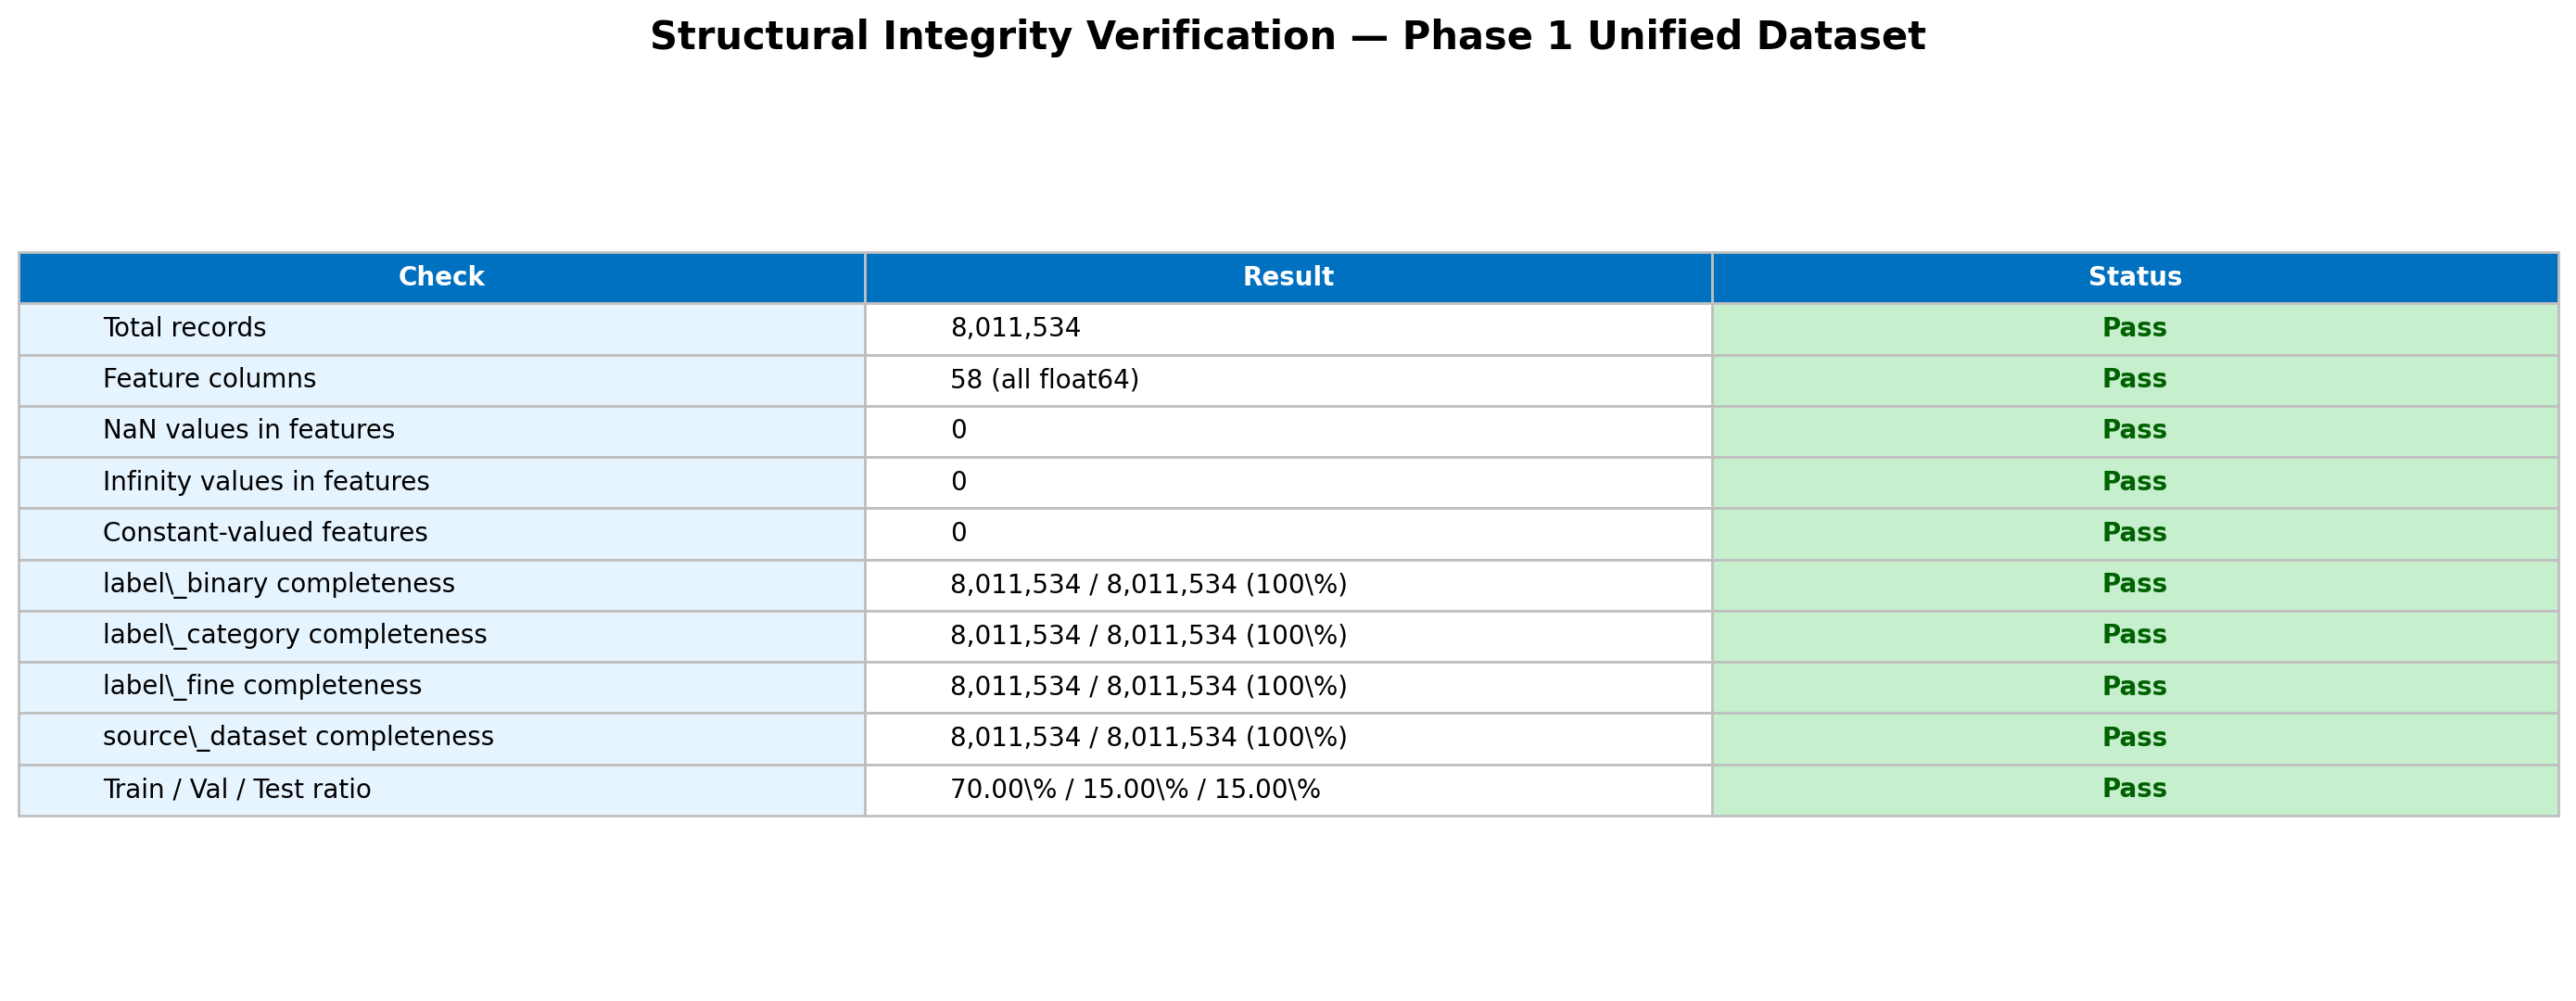
\includegraphics[width=0.9\textwidth]{structural_integrity_check.png}
\caption{Structural integrity verification results. All checks pass, confirming the dataset is well-formed and ready for model training.}
\label{fig:structural-integrity}
\end{figure}

\subsection{Feature Distribution Analysis}
\label{subsec:feature-distributions}

This subsection examines the statistical properties of the 58 scaled features to verify that the standardization process preserved informational content and to characterize the distributional landscape that downstream models will encounter.

\paragraph{Scaling correctness.}
On the training partition, the per-feature means are effectively zero ($\overline{\mu} \approx 1 \times 10^{-8}$) and standard deviations are exactly 1.0, confirming correct \texttt{StandardScaler} behavior. On the validation and test partitions, the maximum absolute mean deviation from zero is 0.0013 and 0.0026 respectively, and the standard deviations remain close to unity. These small deviations are expected and \textit{desirable}: they confirm that no information from the validation/test sets leaked into the scaling parameters.

\paragraph{Distribution shape.}
The majority of features exhibit heavy-tailed, non-Gaussian distributions: 52 of the 58 features have $|\text{skewness}| > 2$ and 51 have kurtosis exceeding 10. This is characteristic of network traffic data, where most flows are short and low-volume but a small fraction of flows (particularly during flood attacks) produce extreme outlier values. The scaled feature range spans from $-13.23$ to $+2{,}368.14$, reflecting these heavy tails. Models must therefore be robust to long-tailed input distributions or employ appropriate techniques (e.g., gradient clipping, robust loss functions).

Figure~\ref{fig:feature-dist-source} shows eight representative features, plotted separately for the two source datasets after scaling. The blue outline corresponds to ``CICIoMT2024'' and the orange outline to ``IoMT-TrafficData''. For each feature, overlapping outlines mean the two sources produce values with similar frequency (similar behaviour), while clearly separated peaks indicate that the feature behaves differently across sources. This figure is useful because it lets us check, at a glance, whether the preprocessing makes the feature values comparable and whether some features carry source-specific patterns that can affect later learning.

\begin{figure}[htbp]
\centering
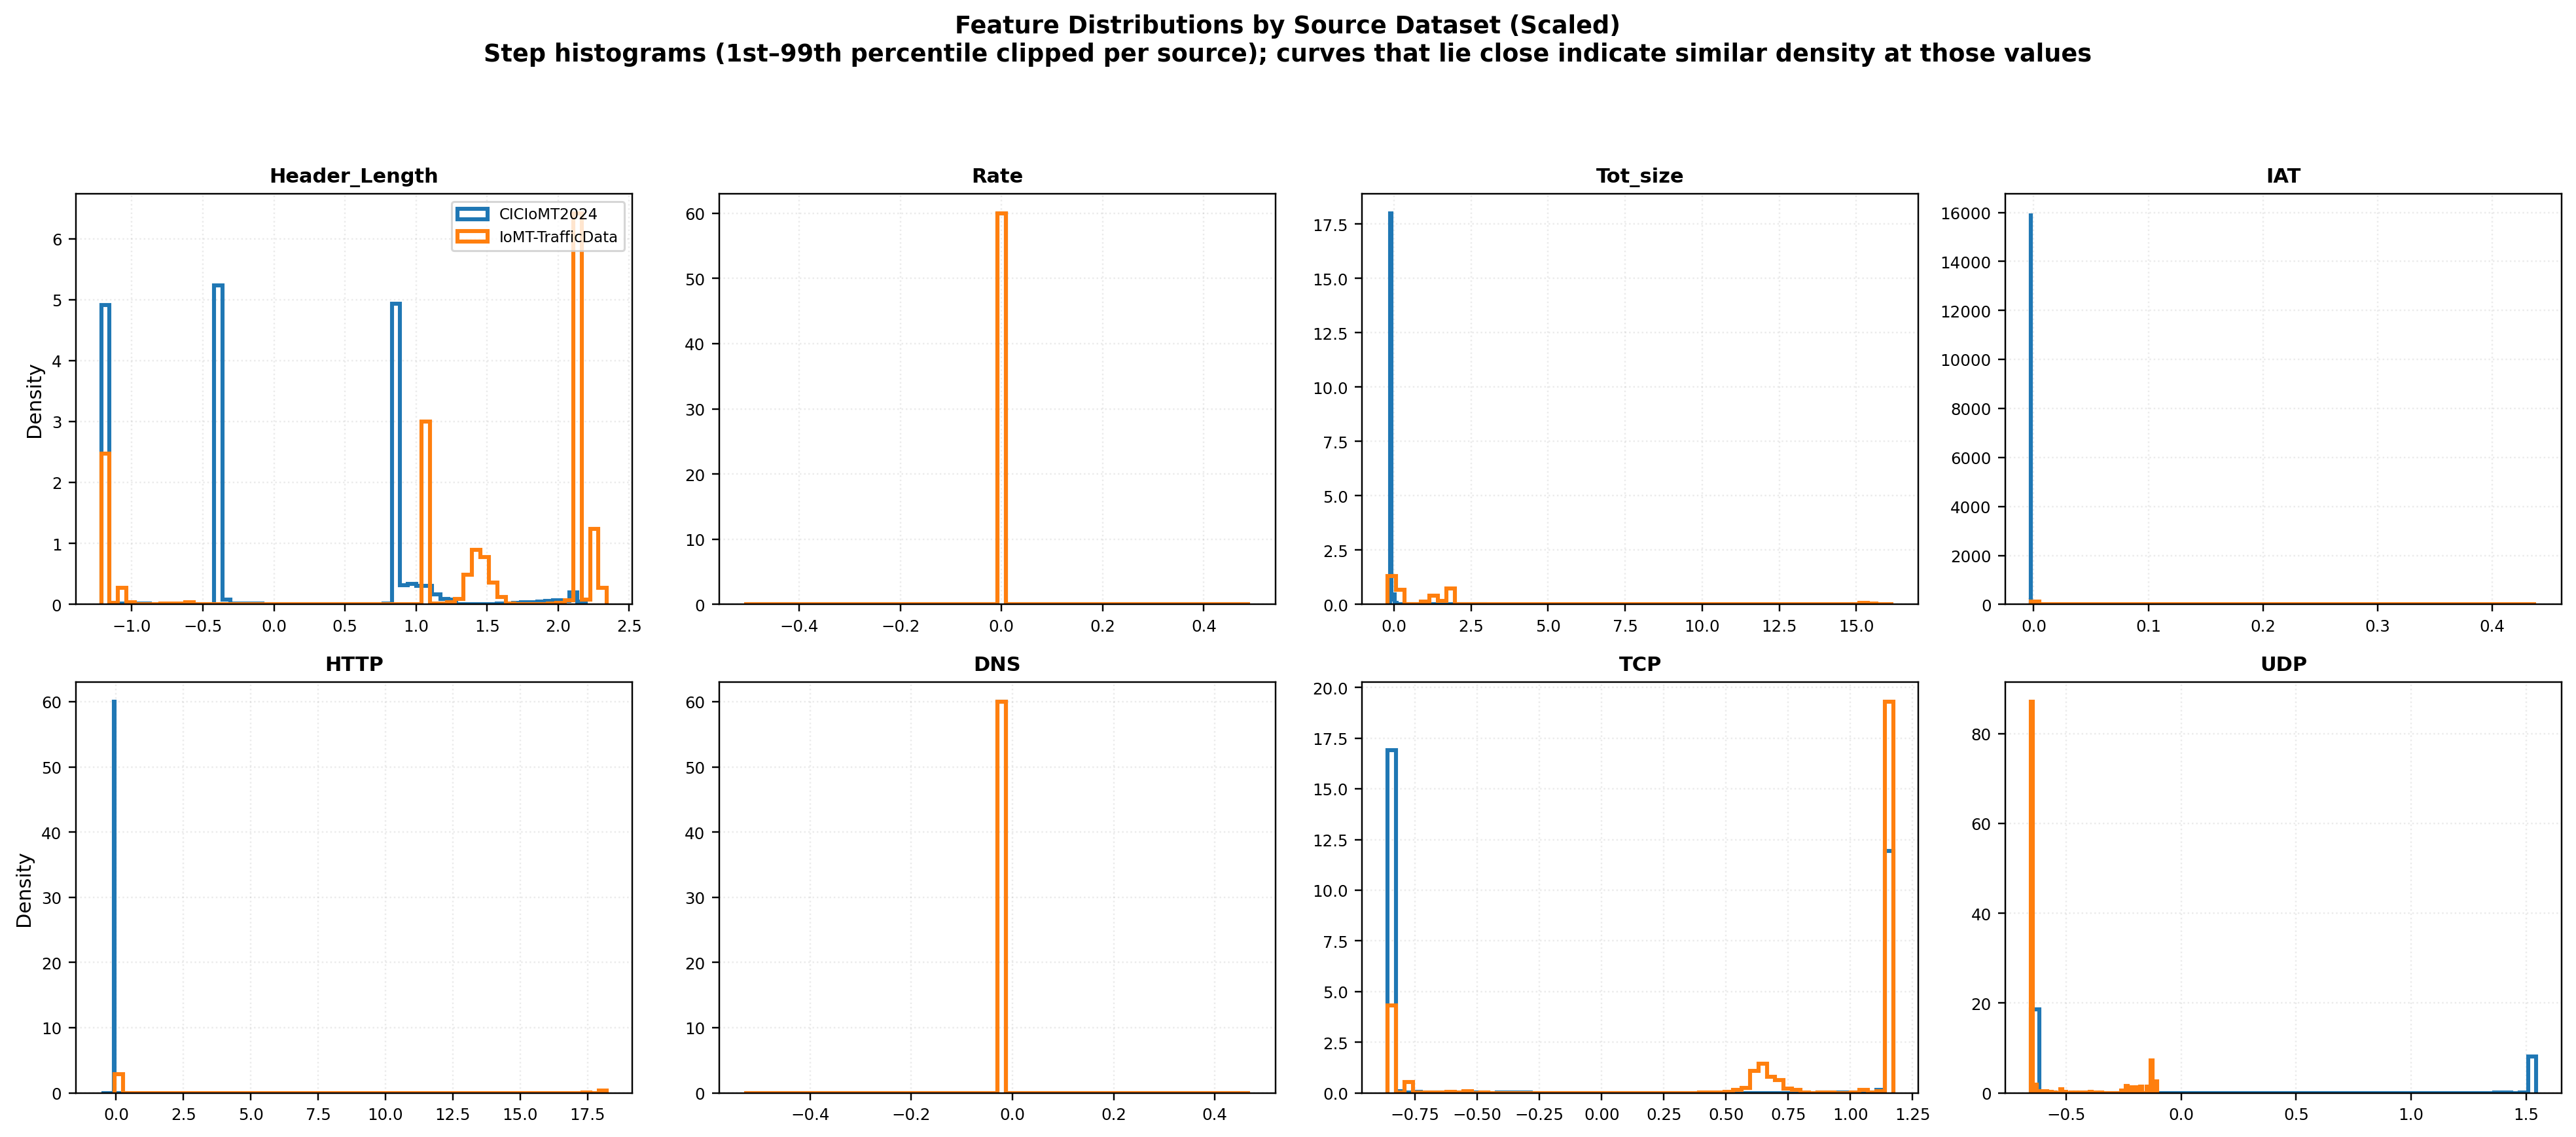
\includegraphics[width=\textwidth]{ch5_feature_distributions_by_source.png}
\caption{Feature distributions after scaling for eight representative features. Blue: CICIoMT2024; orange: IoMT-TrafficData. Overlap suggests similar value frequencies across sources, while separated peaks indicate source-specific behaviour.}
\label{fig:feature-dist-source}
\end{figure}

Figure~\ref{fig:scaling-verification} provides a global view of the scaling quality: per-feature means and standard deviations are plotted for all three partitions. The training set (green) adheres tightly to the theoretical targets of 0 and 1, while the validation and test sets (blue, red) exhibit only minimal deviations, as expected from correctly applied train-only scaling.

\begin{figure}[H]
\centering
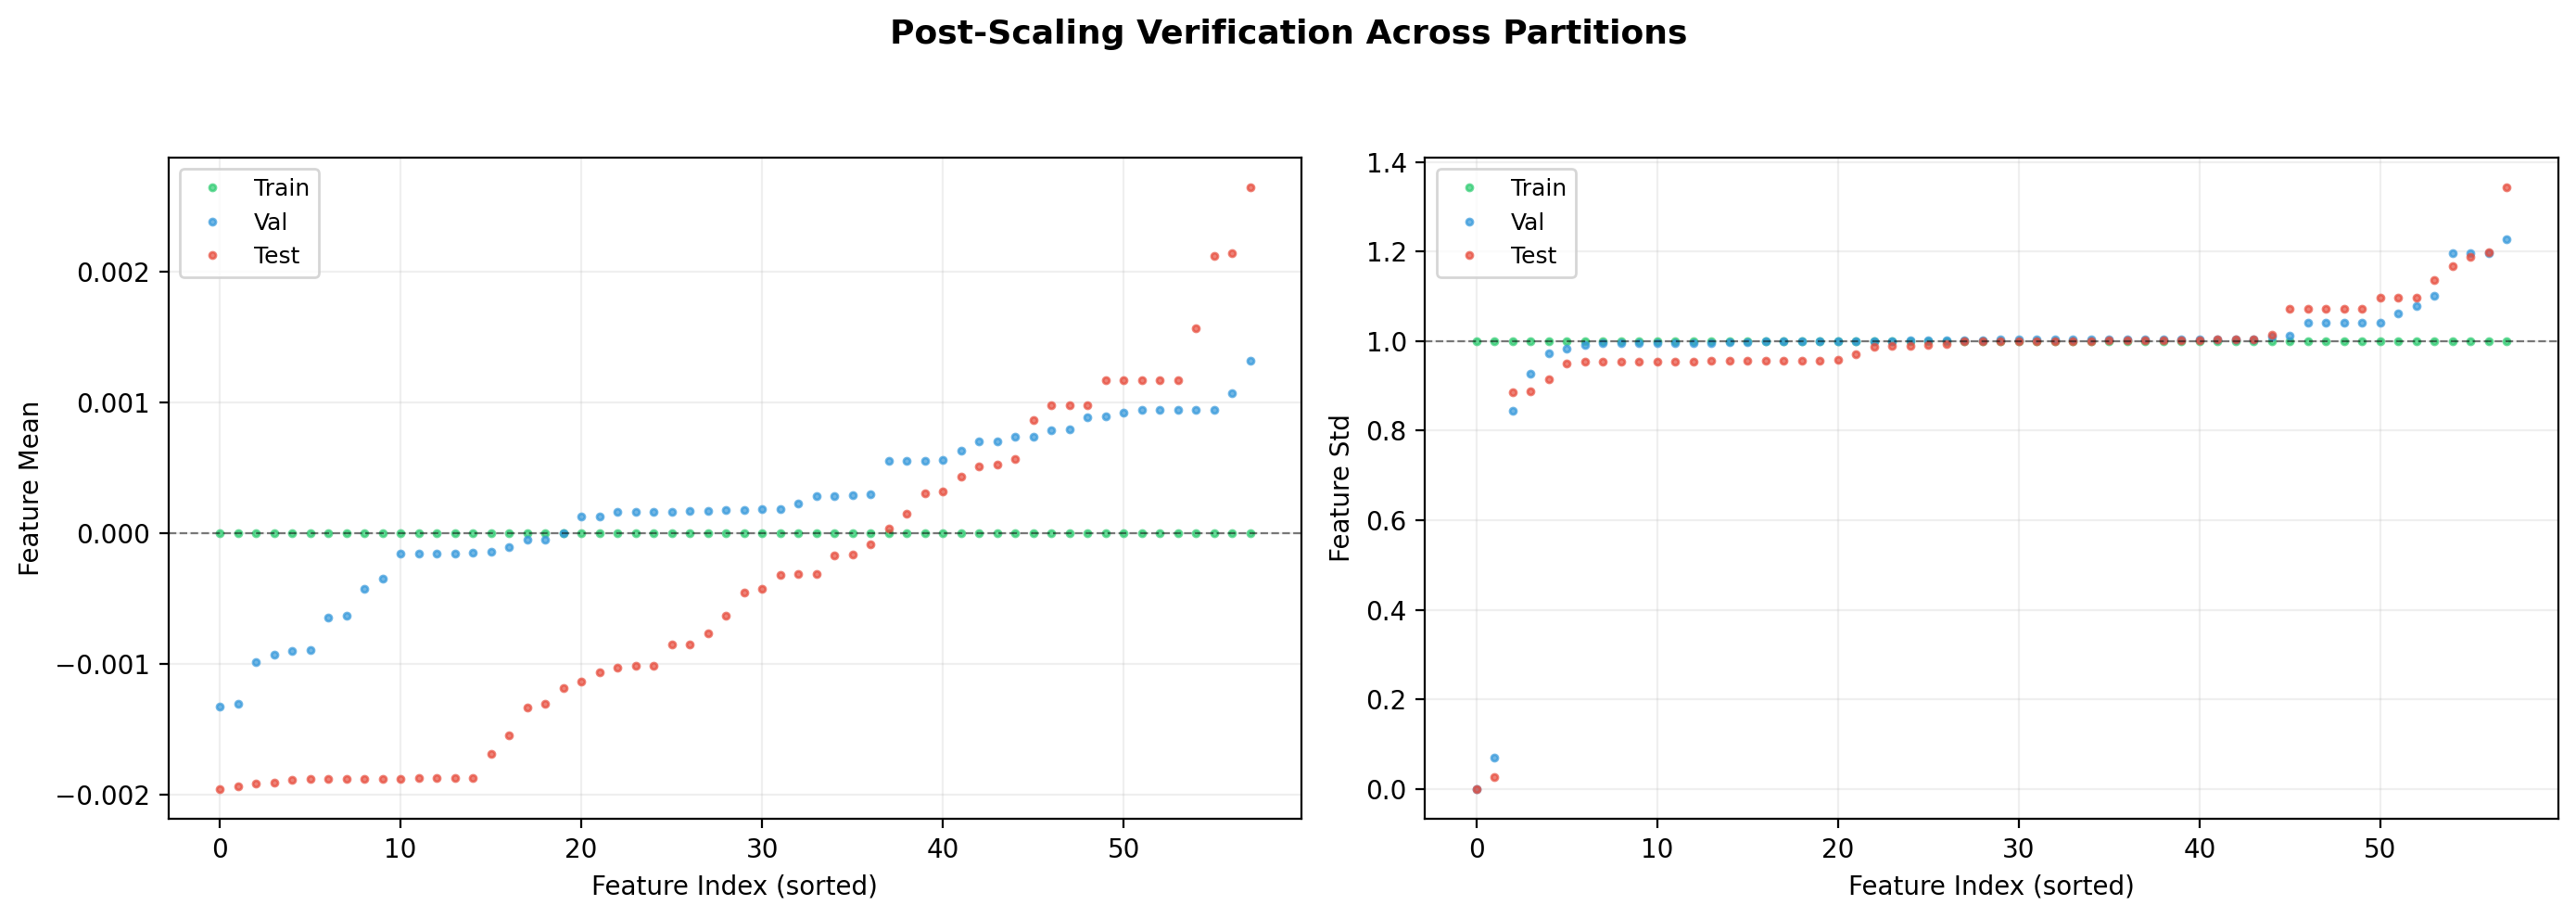
\includegraphics[width=\textwidth]{ch5_scaling_verification.png}
\caption{Post-scaling verification. Left: per-feature means across all three partitions. Right: per-feature standard deviations. The training set matches the theoretical targets exactly; validation/test deviations are minimal, confirming no data leakage.}
\label{fig:scaling-verification}
\end{figure}
\FloatBarrier

\subsection{Class Balance Assessment}
\label{subsec:class-balance}

Class imbalance is a critical consideration for intrusion detection datasets, as it directly affects model training dynamics, evaluation metric interpretation, and operational deployment decisions. This subsection quantifies the imbalance at all three label granularities.

\paragraph{Binary level.}
The dataset is heavily attack-dominated: 7,958,078 records (99.33\%) are labeled \texttt{Attack} and only 53,456 (0.67\%) are \texttt{Benign}. This approximately 149:1 ratio reflects the experimental design of both source datasets, which were constructed to comprehensively capture attack traffic rather than to model realistic benign-to-attack ratios.

\paragraph{Category level.}
Six categories exhibit substantial imbalance, with a maximum-to-minimum ratio of approximately 575:1 (DDoS vs.\ Spoofing). Table~\ref{tab:class-balance} provides the full distribution. The Shannon entropy of the category distribution is 1.209 out of a theoretical maximum of 2.585 (for a uniform 6-class distribution), yielding a normalized entropy of 0.468---indicating moderate concentration. DDoS and DoS together account for 93.83\% of all records, while the remaining four categories collectively represent only 6.17\%.

\begin{table}[H]
\centering
\caption{Category-level class distribution in the final Phase~1 dataset.}
\label{tab:class-balance}
\small
\begin{tabular}{@{}l r r@{}}
\toprule
\textbf{Category} & \textbf{Records} & \textbf{Proportion} \\
\midrule
DDoS & 5,368,292 & 67.01\% \\
DoS & 2,148,477 & 26.82\% \\
MQTT & 385,938 & 4.82\% \\
Benign & 53,456 & 0.67\% \\
Reconnaissance & 46,026 & 0.57\% \\
Spoofing & 9,345 & 0.12\% \\
\midrule
\textbf{Total} & \textbf{8,011,534} & \textbf{100\%} \\
\bottomrule
\end{tabular}
\end{table}

\paragraph{Fine-grained level.}
At the most detailed level, 26 distinct attack types span four orders of magnitude: \texttt{TCP\_IP-DDoS-ICMP} (1,739,060 records) is the most frequent, while \texttt{Recon-Ping\_Sweep} (94 records) is the rarest, yielding an extreme imbalance ratio of approximately 18,500:1. This level of imbalance makes fine-grained classification challenging and motivates the use of class-weighted losses, oversampling, or hierarchical classification strategies in subsequent experiments.

\paragraph{Stratification verification.}
The stratified splitting successfully preserves category proportions across all three partitions. Figure~\ref{fig:class-balance} confirms that per-category percentages are virtually identical in the train, validation, and test sets, ensuring that evaluation metrics reflect genuine model performance rather than partition-level distributional artifacts.

\begin{figure}[htbp]
\centering
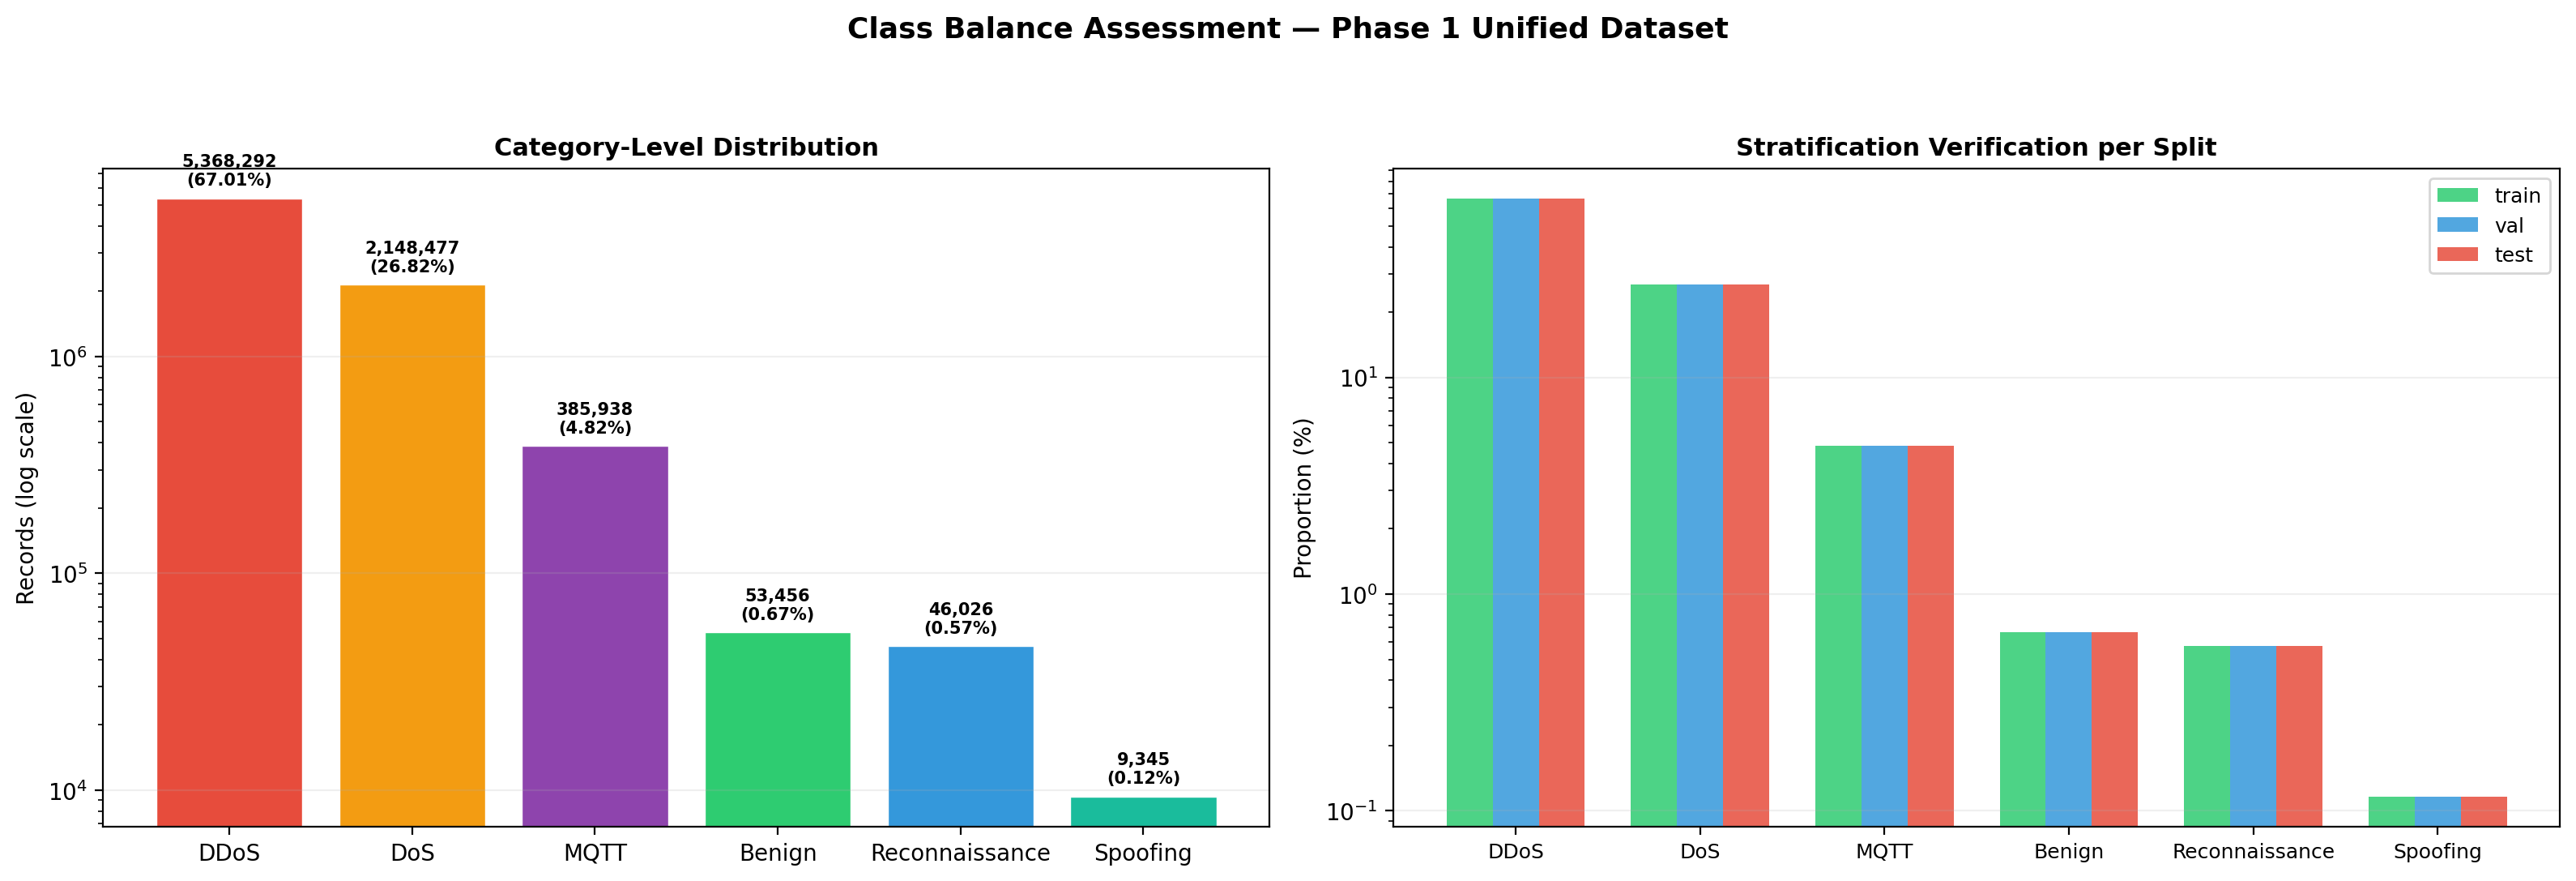
\includegraphics[width=\textwidth]{ch5_class_balance.png}
\caption{Class balance assessment. Left: category-level distribution (log scale) with absolute counts and percentages. Right: per-split category proportions confirming successful stratification.}
\label{fig:class-balance}
\end{figure}

\paragraph{Implications for model training.}
The observed imbalance necessitates careful metric selection: overall accuracy would be misleadingly high due to majority-class dominance. Instead, macro-averaged F1-score and per-class recall will serve as primary evaluation metrics in Section~\ref{sec:model-evaluation}, and class-weighted loss functions will be employed during training to ensure that minority categories (Spoofing, Reconnaissance, Benign) receive adequate gradient signal.

\subsection{Cross-Source Consistency Analysis}
\label{subsec:cross-source}

The unified dataset integrates traffic from two fundamentally different IoMT environments---CICIoMT2024 (a large-scale multi-device testbed) and IoMT-TrafficData (a hospital-oriented testbed). This subsection examines whether source-specific distributional differences are preserved (a desirable property for generalization) versus whether integration introduced artificial artifacts.

\paragraph{Feature-level statistics.}
The two sources exhibit meaningfully different feature-level statistics. CICIoMT2024 records have a mean-of-means of $-0.014$ and a mean-of-standard-deviations of $0.807$ across the 58 features, while IoMT-TrafficData records show a mean-of-means of $0.602$ and a mean-of-standard-deviations of $2.338$. The higher variance in IoMT-TrafficData is expected: as the smaller dataset (2.30\% of records), its records are drawn from a more diverse set of attack methodologies relative to its size, and the scaler was fitted predominantly on CICIoMT2024 traffic.

\paragraph{Category composition.}
The two sources contribute qualitatively different category profiles (see Section~\ref{subsec:label-distributions}). CICIoMT2024 is dominated by DDoS (68.58\%) and DoS (26.84\%), with MQTT, Reconnaissance, Benign, and Spoofing each contributing less than 5\%. IoMT-TrafficData has a more balanced distribution: MQTT (35.68\%), DoS (25.91\%), Reconnaissance (17.85\%), Benign (16.46\%), and Spoofing (4.10\%)---and no DDoS traffic at all. This complementarity is by design and is the core motivation for integration.

\paragraph{Shared fine-grained labels.}
Two fine-grained attack types appear in both datasets: \texttt{Benign} and \texttt{ARP\_Spoofing}. These shared labels enable direct cross-environment comparison for the same attack/traffic type, providing a built-in benchmark for evaluating whether a model can generalize the detection of identical attacks across different network infrastructures.

\paragraph{PCA visualization.}
Figure~\ref{fig:pca-cross-source} is a 2D projection of the unified dataset obtained with PCA. Each point corresponds to one record. The left panel colors points by source dataset (CICIoMT2024 vs. IoMT-TrafficData), while the right panel colors points by attack category. Points that group together indicate records with similar patterns in the reduced feature space; mixing between colours suggests overlap between groups. This figure is useful as a qualitative check: it helps us see whether the sources are represented in a similar feature space (supporting unified learning) and whether attack categories create distinguishable structure that the models can potentially learn.

\begin{figure}[htbp]
\centering
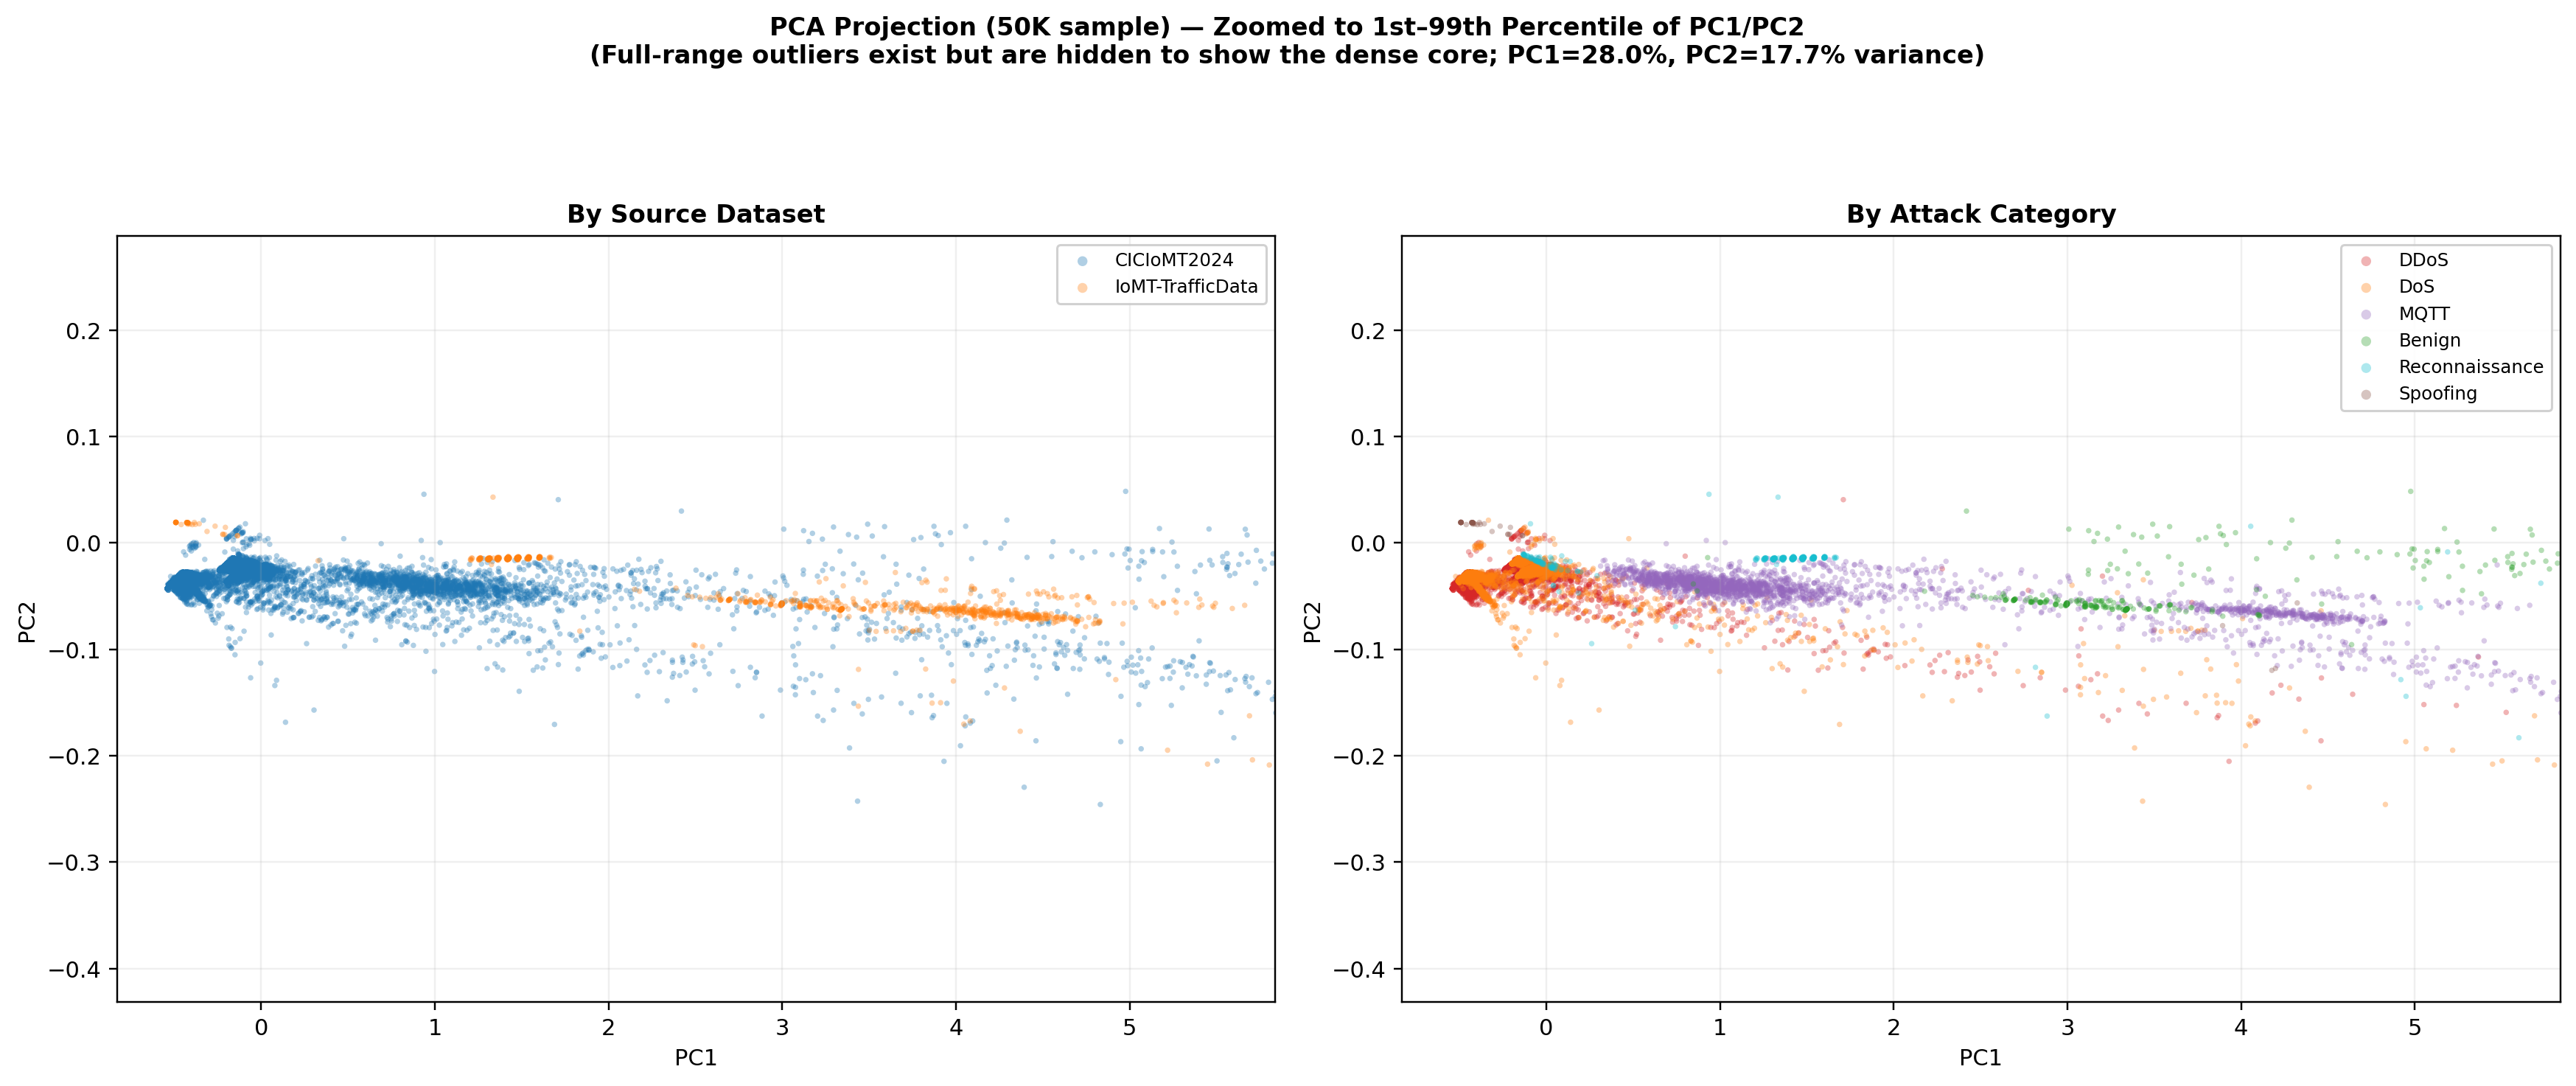
\includegraphics[width=\textwidth]{ch5_pca_cross_source.png}
\caption{PCA projection of a 50K sample from the unified dataset. Left: points colored by source dataset. Right: points colored by attack category. The grouping pattern indicates similarity in the reduced feature space.}
\label{fig:pca-cross-source}
\end{figure}

\paragraph{Assessment summary.}
The cross-source analysis confirms that the integration pipeline successfully preserved the genuine distributional differences between the two IoMT environments without introducing artificial artifacts. The partial overlap in PCA space indicates that models trained on the unified dataset can leverage shared structure across sources while also learning source-specific patterns---precisely the outcome that motivates multi-source integration for improved generalizability.

% ══════════════════════════════════════════════════════════════════════════════
\section{IDS Model Evaluation}
\label{sec:model-evaluation}

This section describes the training, comparison, and evaluation of \gls{ids} models on the unified Phase~1 dataset (dedicated MQTT category mapping, \texttt{StandardScaler} preprocessing as described in Chapter~\ref{ch:execution}). It is placed before the research-question synthesis so that empirical results are available when interpreting integration benefits.

\subsection{Experimental Setup}
\label{subsec:experimental-setup}

The experimental framework is designed to answer the central research question: \emph{does training on the unified multi-source dataset improve generalizability compared to training on each source in isolation?} The protocol follows the methodological recommendations of Lones~\cite{lones2024avoid} and is summarized below.

\paragraph{Algorithm selection.}
Three tree-based classifiers of increasing complexity are evaluated: Decision Tree (DT), Random Forest (RF), and XGBoost. Tree-based models are chosen because they have been shown to outperform deep learning on typical tabular datasets~\cite{grinsztajn2022tree}, and because they natively handle multi-class classification without requiring one-vs-rest wrappers.

\paragraph{Target encoding.}
The six attack categories (\texttt{Benign}, \texttt{DDoS}, \texttt{DoS}, \texttt{MQTT}, \texttt{Reconnaissance}, \texttt{Spoofing}) are encoded as integers 0--5 via \texttt{LabelEncoder}. One-hot encoding of the target variable is deliberately avoided: it would transform the problem into a multi-label setting, which is semantically incorrect for mutually exclusive attack categories. One-hot encoding of features is unnecessary because all 58 input features are already numeric (\texttt{float64}). Tree-based models perform splits per class and do not interpret ordinal relationships among integer target labels, so the choice of LabelEncoder introduces no implicit ordering bias.

A \textbf{global} label mapping (alphabetically sorted across all six categories) is used for all training regimes. This ensures that integer labels are consistent across regimes and that confusion matrices from different experiments are directly comparable---even when a regime's training set does not contain all six classes (e.g., B2 lacks DDoS).

\paragraph{Class imbalance handling.}
The dataset exhibits a 575:1 maximum-to-minimum class ratio (Section~\ref{subsec:class-balance}). For Decision Tree and Random Forest, balanced class weights are applied: each class receives a weight of $n_{\text{samples}} / (n_{\text{classes}} \times n_{\text{class}})$, computed by scikit-learn's \texttt{class\_weight='balanced'} parameter. For XGBoost, equivalent per-sample weights are passed via the \texttt{sample\_weight} argument, as \texttt{scale\_pos\_weight} only applies to binary classification. Synthetic oversampling (e.g., SMOTE) is not used, as the dataset already contains over 8 million records and class weights provide sufficient gradient signal for minority classes.

\paragraph{Training regimes.}
To isolate the effect of dataset integration, three training regimes share the same tuning budget, search space, and evaluation protocol---the only variable is which rows of the training set are used:

\begin{itemize}[nosep]
  \item \textbf{B1 (CIC-only)}: Only rows with \texttt{source\_dataset = CICIoMT2024}.
  \item \textbf{B2 (IoMT-only)}: Only rows with \texttt{source\_dataset = IoMT-TrafficData}.
  \item \textbf{U (Unified)}: The complete training set (both sources).
\end{itemize}

The filtering is applied to the existing stratified splits (train/val/test), preserving the original non-overlapping partition boundaries. This design ensures that any performance difference is attributable solely to the training data composition, not to differences in preprocessing, feature engineering, or evaluation procedure.

\paragraph{Hyperparameter tuning.}
\texttt{RandomizedSearchCV} is used with $n_{\text{iter}}=50$, 3-fold \texttt{StratifiedKFold} cross-validation on the training set, and \texttt{scoring='f1\_macro'}. The Decision Tree search space includes depth, split/leaf thresholds, split criterion, and \texttt{max\_features} (full Cartesian grids are defined as constants in the Phase~2 training module). Random Forest adds \texttt{n\_estimators}, \texttt{max\_samples} (bootstrap row fraction per tree, also acting as a memory cap), and \texttt{class\_weight} modes. XGBoost searches learning rate, boosting rounds, tree depth, \texttt{min\_child\_weight}, row and column subsampling, $\gamma$, and $\ell_1/\ell_2$ penalties; training uses \texttt{tree\_method='hist'} and \texttt{objective='multi:softmax'} with per-sample weights (see the class-imbalance paragraph under this subsection). Each regime receives the same iteration budget for fair comparison~\cite{lones2024avoid}.

\paragraph{Feasibility of ensemble tuning on large partitions.}
Full \texttt{RandomizedSearchCV} with wide search spaces over hundreds of thousands of training rows and hundreds of trees per candidate is computationally heavy on a single workstation. For Random Forest and XGBoost only, hyperparameter search is therefore performed on a \emph{stratified random subsample} of 300{,}000 training rows whenever the regime's training partition exceeds that size (B1 and U); B2 remains below this threshold and uses the full IoMT-only training set. The best hyperparameter vector from this search is then used to train a final model on the \emph{complete} training partition before the locked test-set evaluation. The held-out test set is still touched only once for reporting; only the inner cross-validation for search uses the subsample. This two-stage procedure is a standard pragmatic compromise in large-scale tabular learning~\cite{lones2024avoid} and keeps the methodology aligned with the Decision Tree protocol aside from this explicit feasibility constraint.

\paragraph{Evaluation protocol.}
Following the ``test set once'' principle (\S4.3 of~\cite{lones2024avoid}), hyperparameters are tuned exclusively on the validation set. The test set is evaluated only once per model to report final metrics, after all tuning decisions are locked. The evaluation matrix covers three test slices per model:

\begin{itemize}[nosep]
  \item \textbf{In-domain}: The test slice matching the training source (e.g., B1 $\to$ CIC test slice).
  \item \textbf{Cross-domain}: The test slice from the \emph{other} source (e.g., B1 $\to$ IoMT test slice).
  \item \textbf{Full}: The complete unified test set.
\end{itemize}

\paragraph{Metrics.}
Overall accuracy is reported only for completeness; it is \textbf{not} used as the primary metric due to severe class imbalance. The primary metric is \textbf{macro-averaged F1-score}, which gives equal weight to each class regardless of its frequency. Weighted F1-score, per-class precision, recall, and F1-score, and normalized confusion matrices are also reported to provide a complete picture. For pairwise model comparison, McNemar's test is applied to the test-set predictions.

\subsection{Decision Tree Classifier}
\label{subsec:decision-tree}

The Decision Tree (DT) classifier serves as the first model in the progressive-complexity sequence (DT $\to$ RF $\to$ XGBoost). Two stages are evaluated per regime: a \emph{baseline} DT with default scikit-learn hyperparameters (only \texttt{class\_weight} set to balanced), and a \emph{tuned} DT with the best hyperparameters from \texttt{RandomizedSearchCV}.

\subsubsection{Baseline Results}

Table~\ref{tab:dt-baseline} reports baseline DT performance across all regime-slice combinations.

\begin{table}[H]
\centering
\caption{Baseline Decision Tree (default hyperparameters) evaluation matrix.}
\label{tab:dt-baseline}
\small
\begin{tabular}{@{}l l c c c@{}}
\toprule
\textbf{Regime} & \textbf{Test slice} & \textbf{Macro-F1} & \textbf{Weighted-F1} & \textbf{Accuracy} \\
\midrule
B1 (CIC-only) & CIC (in-domain)  & 0.9119 & 0.8667 & 0.8668 \\
B1 (CIC-only) & IoMT (cross)     & 0.2256 & 0.3849 & 0.3816 \\
B1 (CIC-only) & Full             & 0.6683 & 0.8542 & 0.8556 \\
\midrule
B2 (IoMT-only) & IoMT (in-domain) & 0.8332 & 0.9998 & 0.9998 \\
B2 (IoMT-only) & CIC (cross)      & 0.0527 & 0.0513 & 0.0617 \\
B2 (IoMT-only) & Full             & 0.3315 & 0.0661 & 0.0833 \\
\midrule
U (Unified)    & CIC              & 0.9143 & 0.8667 & 0.8668 \\
U (Unified)    & IoMT             & 0.8329 & 0.9994 & 0.9993 \\
U (Unified)    & Full             & \textbf{0.9366} & 0.8697 & 0.8699 \\
\bottomrule
\end{tabular}
\end{table}
\FloatBarrier

\subsubsection{Tuned Results}

Table~\ref{tab:dt-tuned} reports the tuned DT results. The best hyperparameters per regime are listed in Table~\ref{tab:dt-best-params}.

\begin{table}[H]
\centering
\caption{Tuned Decision Tree evaluation matrix.}
\label{tab:dt-tuned}
\small
\begin{tabular}{@{}l l c c c@{}}
\toprule
\textbf{Regime} & \textbf{Test slice} & \textbf{Macro-F1} & \textbf{Weighted-F1} & \textbf{Accuracy} \\
\midrule
Tuned B1 & CIC (in-domain)  & 0.9226 & 0.8889 & 0.8853 \\
Tuned B1 & IoMT (cross)     & 0.2474 & 0.3923 & 0.3892 \\
Tuned B1 & Full             & 0.6959 & 0.8769 & 0.8738 \\
\midrule
Tuned B2 & IoMT (in-domain) & 0.8332 & 0.9999 & 0.9999 \\
Tuned B2 & CIC (cross)      & 0.0523 & 0.0619 & 0.0570 \\
Tuned B2 & Full             & 0.3284 & 0.0756 & 0.0787 \\
\midrule
Tuned U  & CIC              & 0.9262 & 0.8899 & 0.8863 \\
Tuned U  & IoMT             & 0.8325 & 0.9990 & 0.9990 \\
Tuned U  & Full             & \textbf{0.9480} & 0.8923 & 0.8889 \\
\bottomrule
\end{tabular}
\end{table}
\FloatBarrier

\paragraph{Note on Macro-F1 interpretation (Table~\ref{tab:dt-tuned}).}
For the Tuned U result on the IoMT slice, the reported Macro-F1 ($0.8325$) is computed over the global six-class label space for consistency across all slices. Because the IoMT slice contains no true DDoS samples (support $=0$), the DDoS class contributes an F1-score of $0$ to the global macro average. If Macro-F1 is computed over present classes only (Benign, DoS, MQTT, Reconnaissance, Spoofing), the value is $0.9990$. Weighted-F1 and accuracy remain $0.9990$ because they are support-weighted and are therefore not penalized by an absent class.

\begin{table}[H]
\centering
\caption{Best hyperparameters per regime (Decision Tree, 50-iteration RandomizedSearchCV).}
\label{tab:dt-best-params}
\small
\begin{tabular}{@{}l c c c c c c@{}}
\toprule
\textbf{Regime} & \textbf{criterion} & \textbf{max\_depth} & \textbf{min\_split} & \textbf{min\_leaf} & \textbf{max\_feat.} & \textbf{CV F1m} \\
\midrule
B1 (CIC-only)  & entropy & 15   & 2 & 2 & None & 0.9232 \\
B2 (IoMT-only) & entropy & 10   & 2 & 1 & None & 0.9998 \\
U (Unified)    & entropy & 15   & 2 & 2 & None & 0.9469 \\
\bottomrule
\end{tabular}
\end{table}

\subsubsection{Cross-Domain Analysis}

The cross-domain evaluation reveals the generalization gap that motivates multi-source integration. When a model trained on only one source (B1 or B2) is evaluated on the other source's test data, performance is expected to degrade---especially for attack categories absent from the training data (e.g., B2 has never seen DDoS traffic).

Figure~\ref{fig:dt-confusion-unified} shows the confusion matrix for the tuned unified DT on the full test set. Figure~\ref{fig:dt-cm-xd} presents the cross-domain confusion matrices that illustrate misclassification patterns when models encounter unseen attack categories.

\begin{figure}[H]
\centering
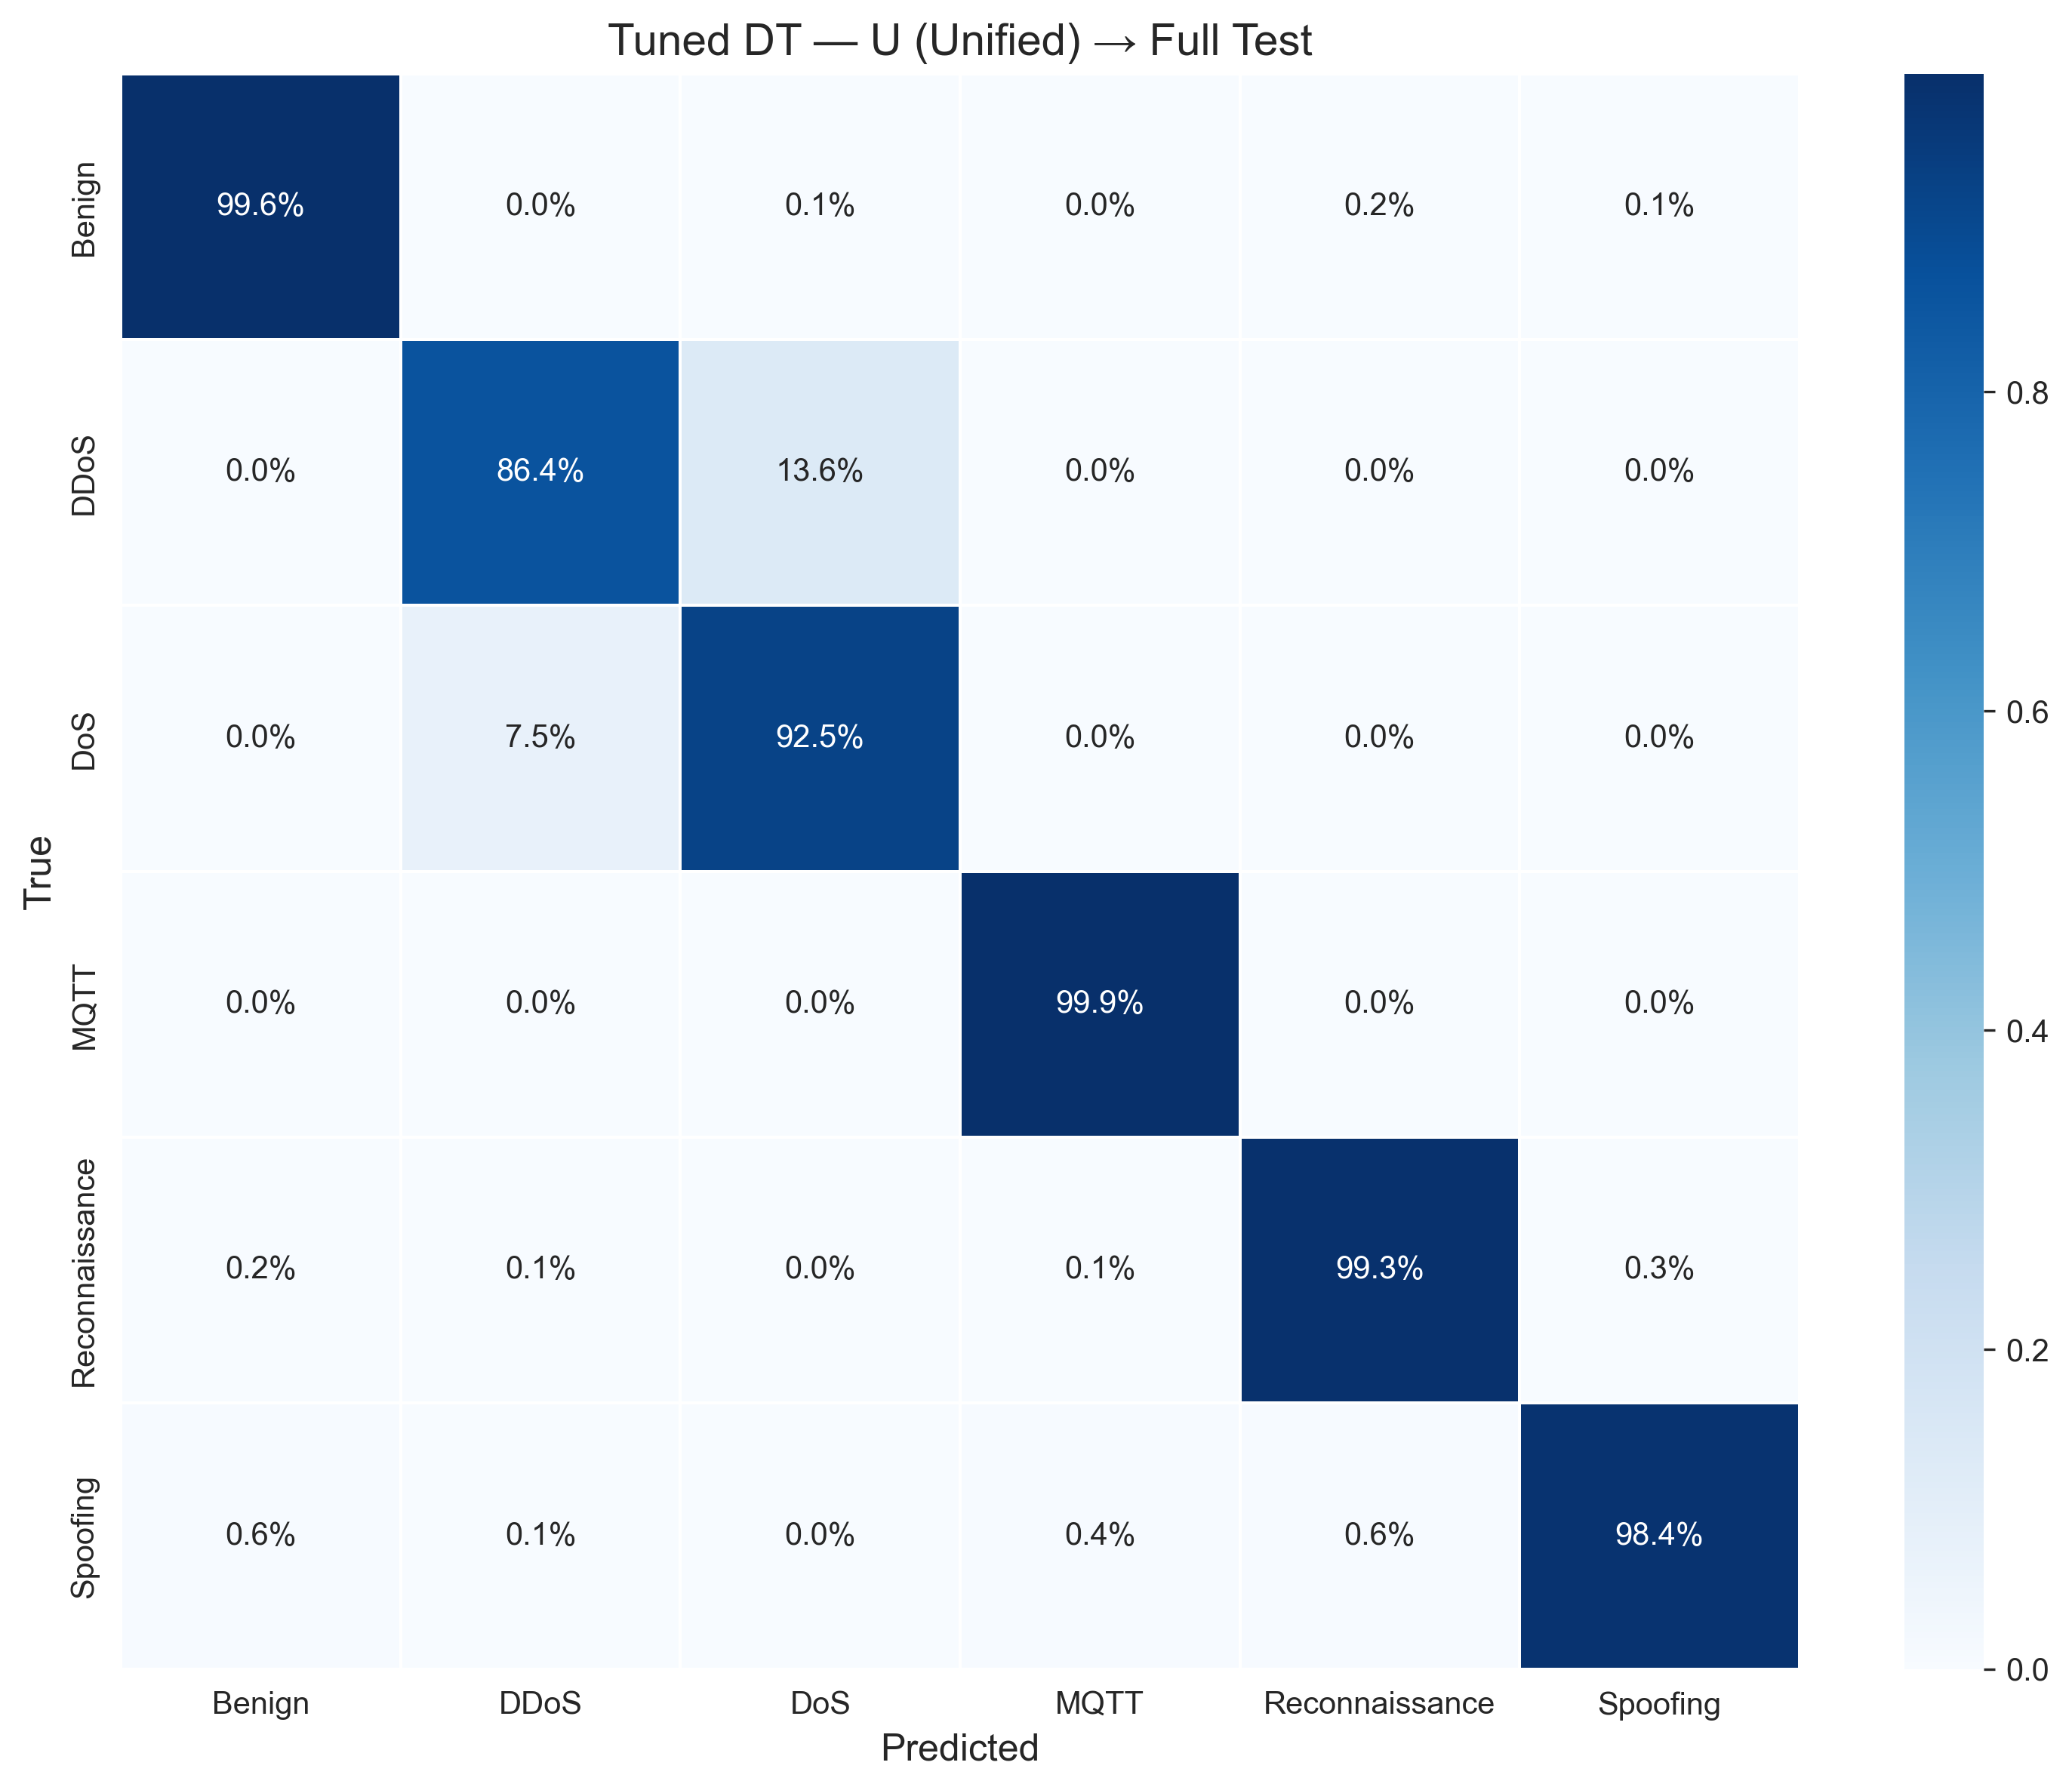
\includegraphics[width=0.75\textwidth]{ch5_dt_cm_u_full.png}
\caption{Normalized confusion matrix --- Tuned DT (Unified) on the full test set.}
\label{fig:dt-confusion-unified}
\end{figure}

\begin{figure}[H]
\centering
\begin{subfigure}[b]{0.48\textwidth}
  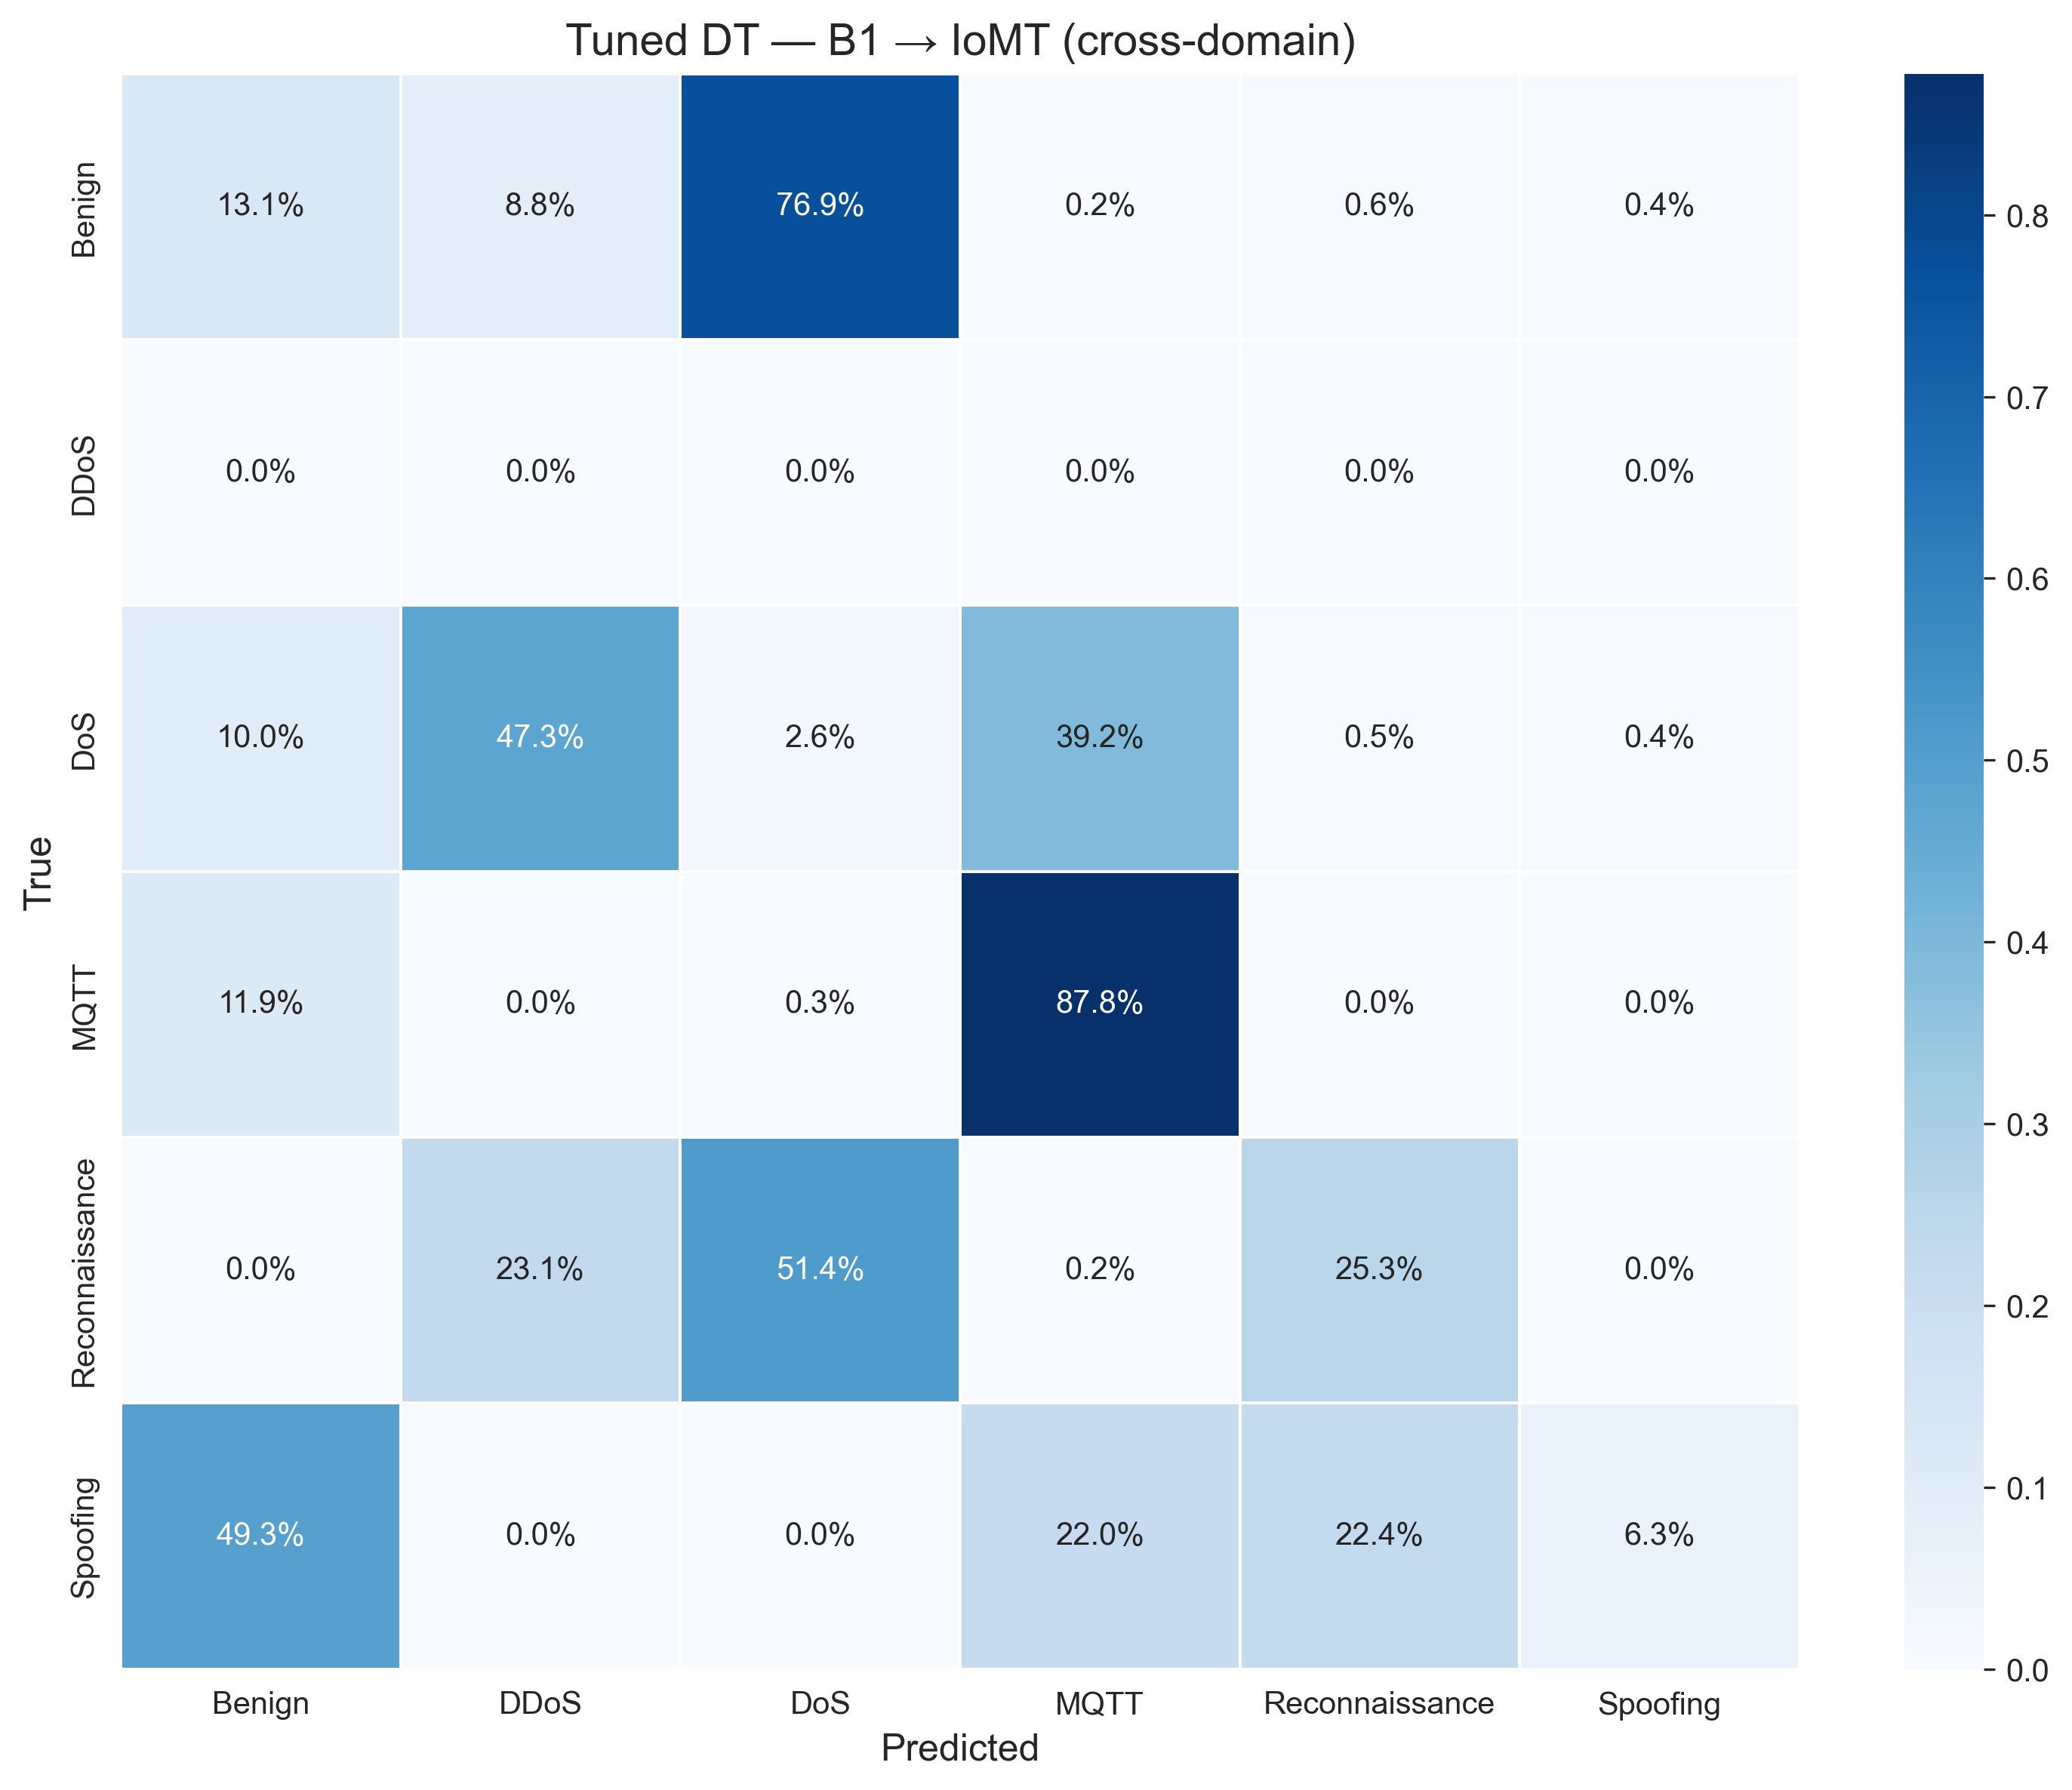
\includegraphics[width=\textwidth]{ch5_dt_cm_b1_xd_iomt.png}
  \caption{B1 (CIC-only) $\to$ IoMT test}
\end{subfigure}
\hfill
\begin{subfigure}[b]{0.48\textwidth}
  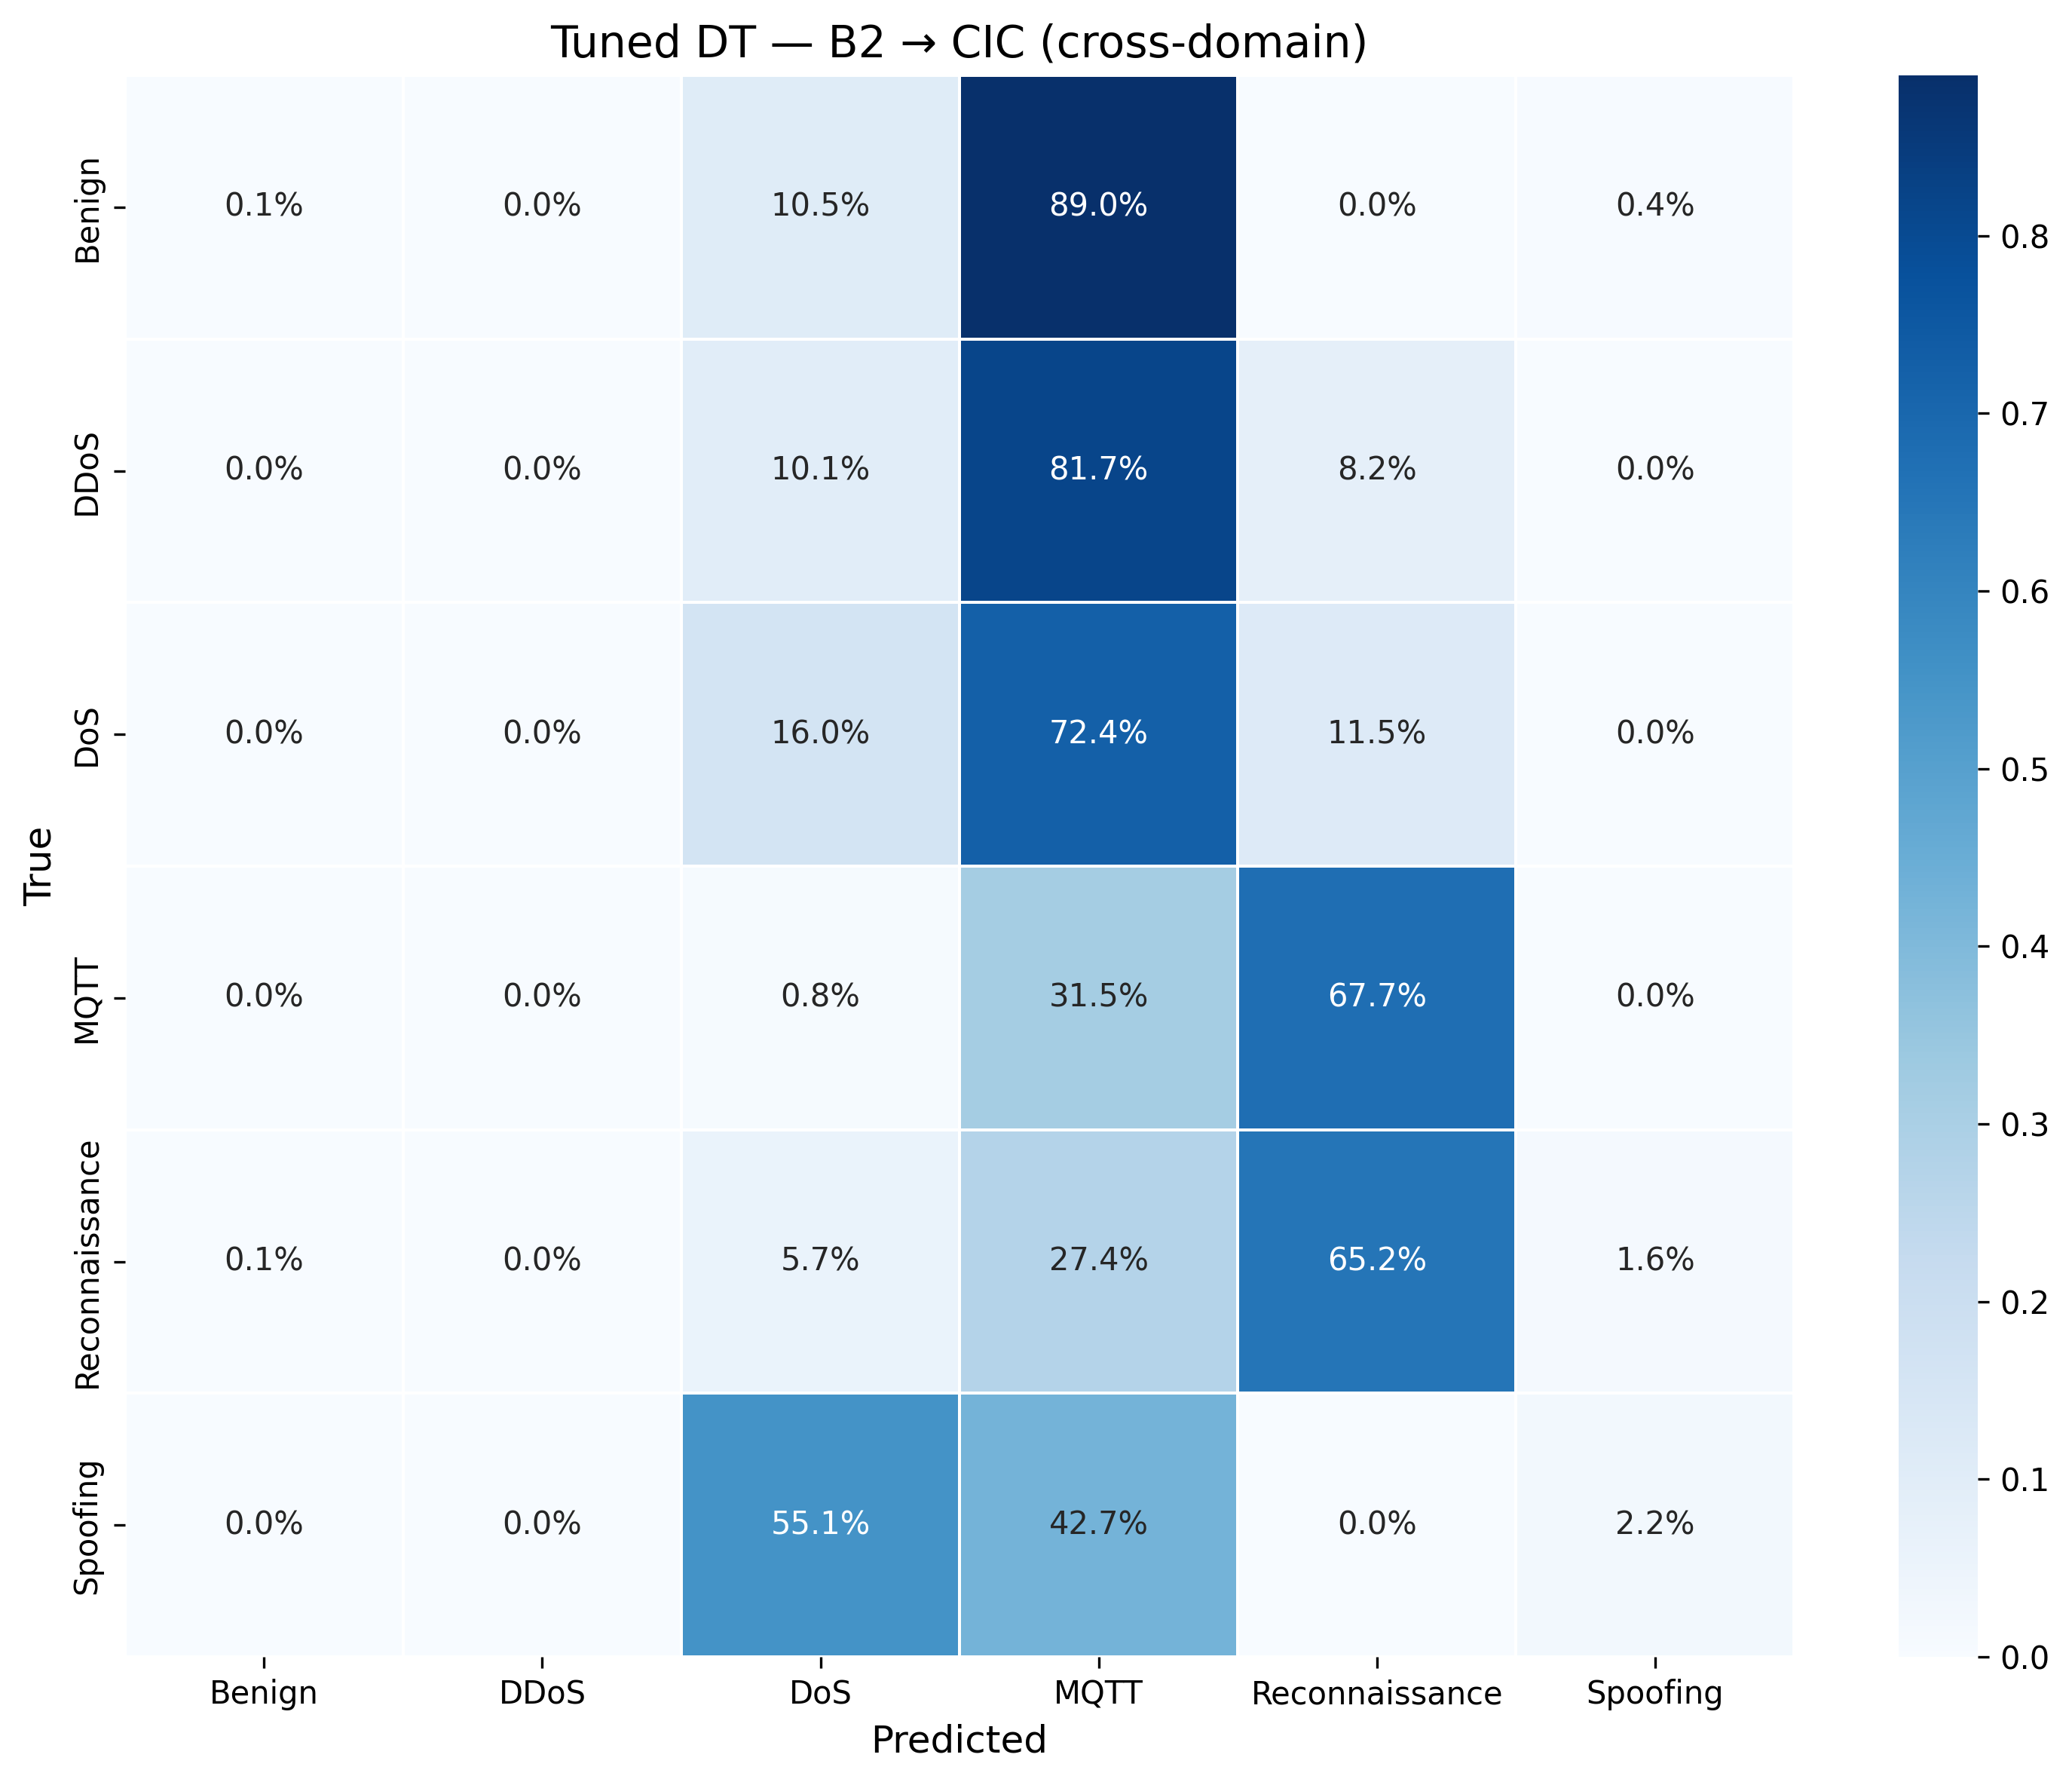
\includegraphics[width=\textwidth]{ch5_dt_cm_b2_xd_cic.png}
  \caption{B2 (IoMT-only) $\to$ CIC test}
\end{subfigure}
\caption{Cross-domain confusion matrices. Single-source models struggle with attack categories absent from their training data.}
\label{fig:dt-cm-xd}
\end{figure}

\subsubsection{Feature Importance}

Figure~\ref{fig:dt-feature-importance} presents the top-20 most important features for the tuned unified DT, measured by Gini importance. Figure~\ref{fig:dt-fi-comparison} compares feature importance rankings across all three regimes, revealing which features are universally discriminative versus source-specific.

\begin{figure}[H]
\centering
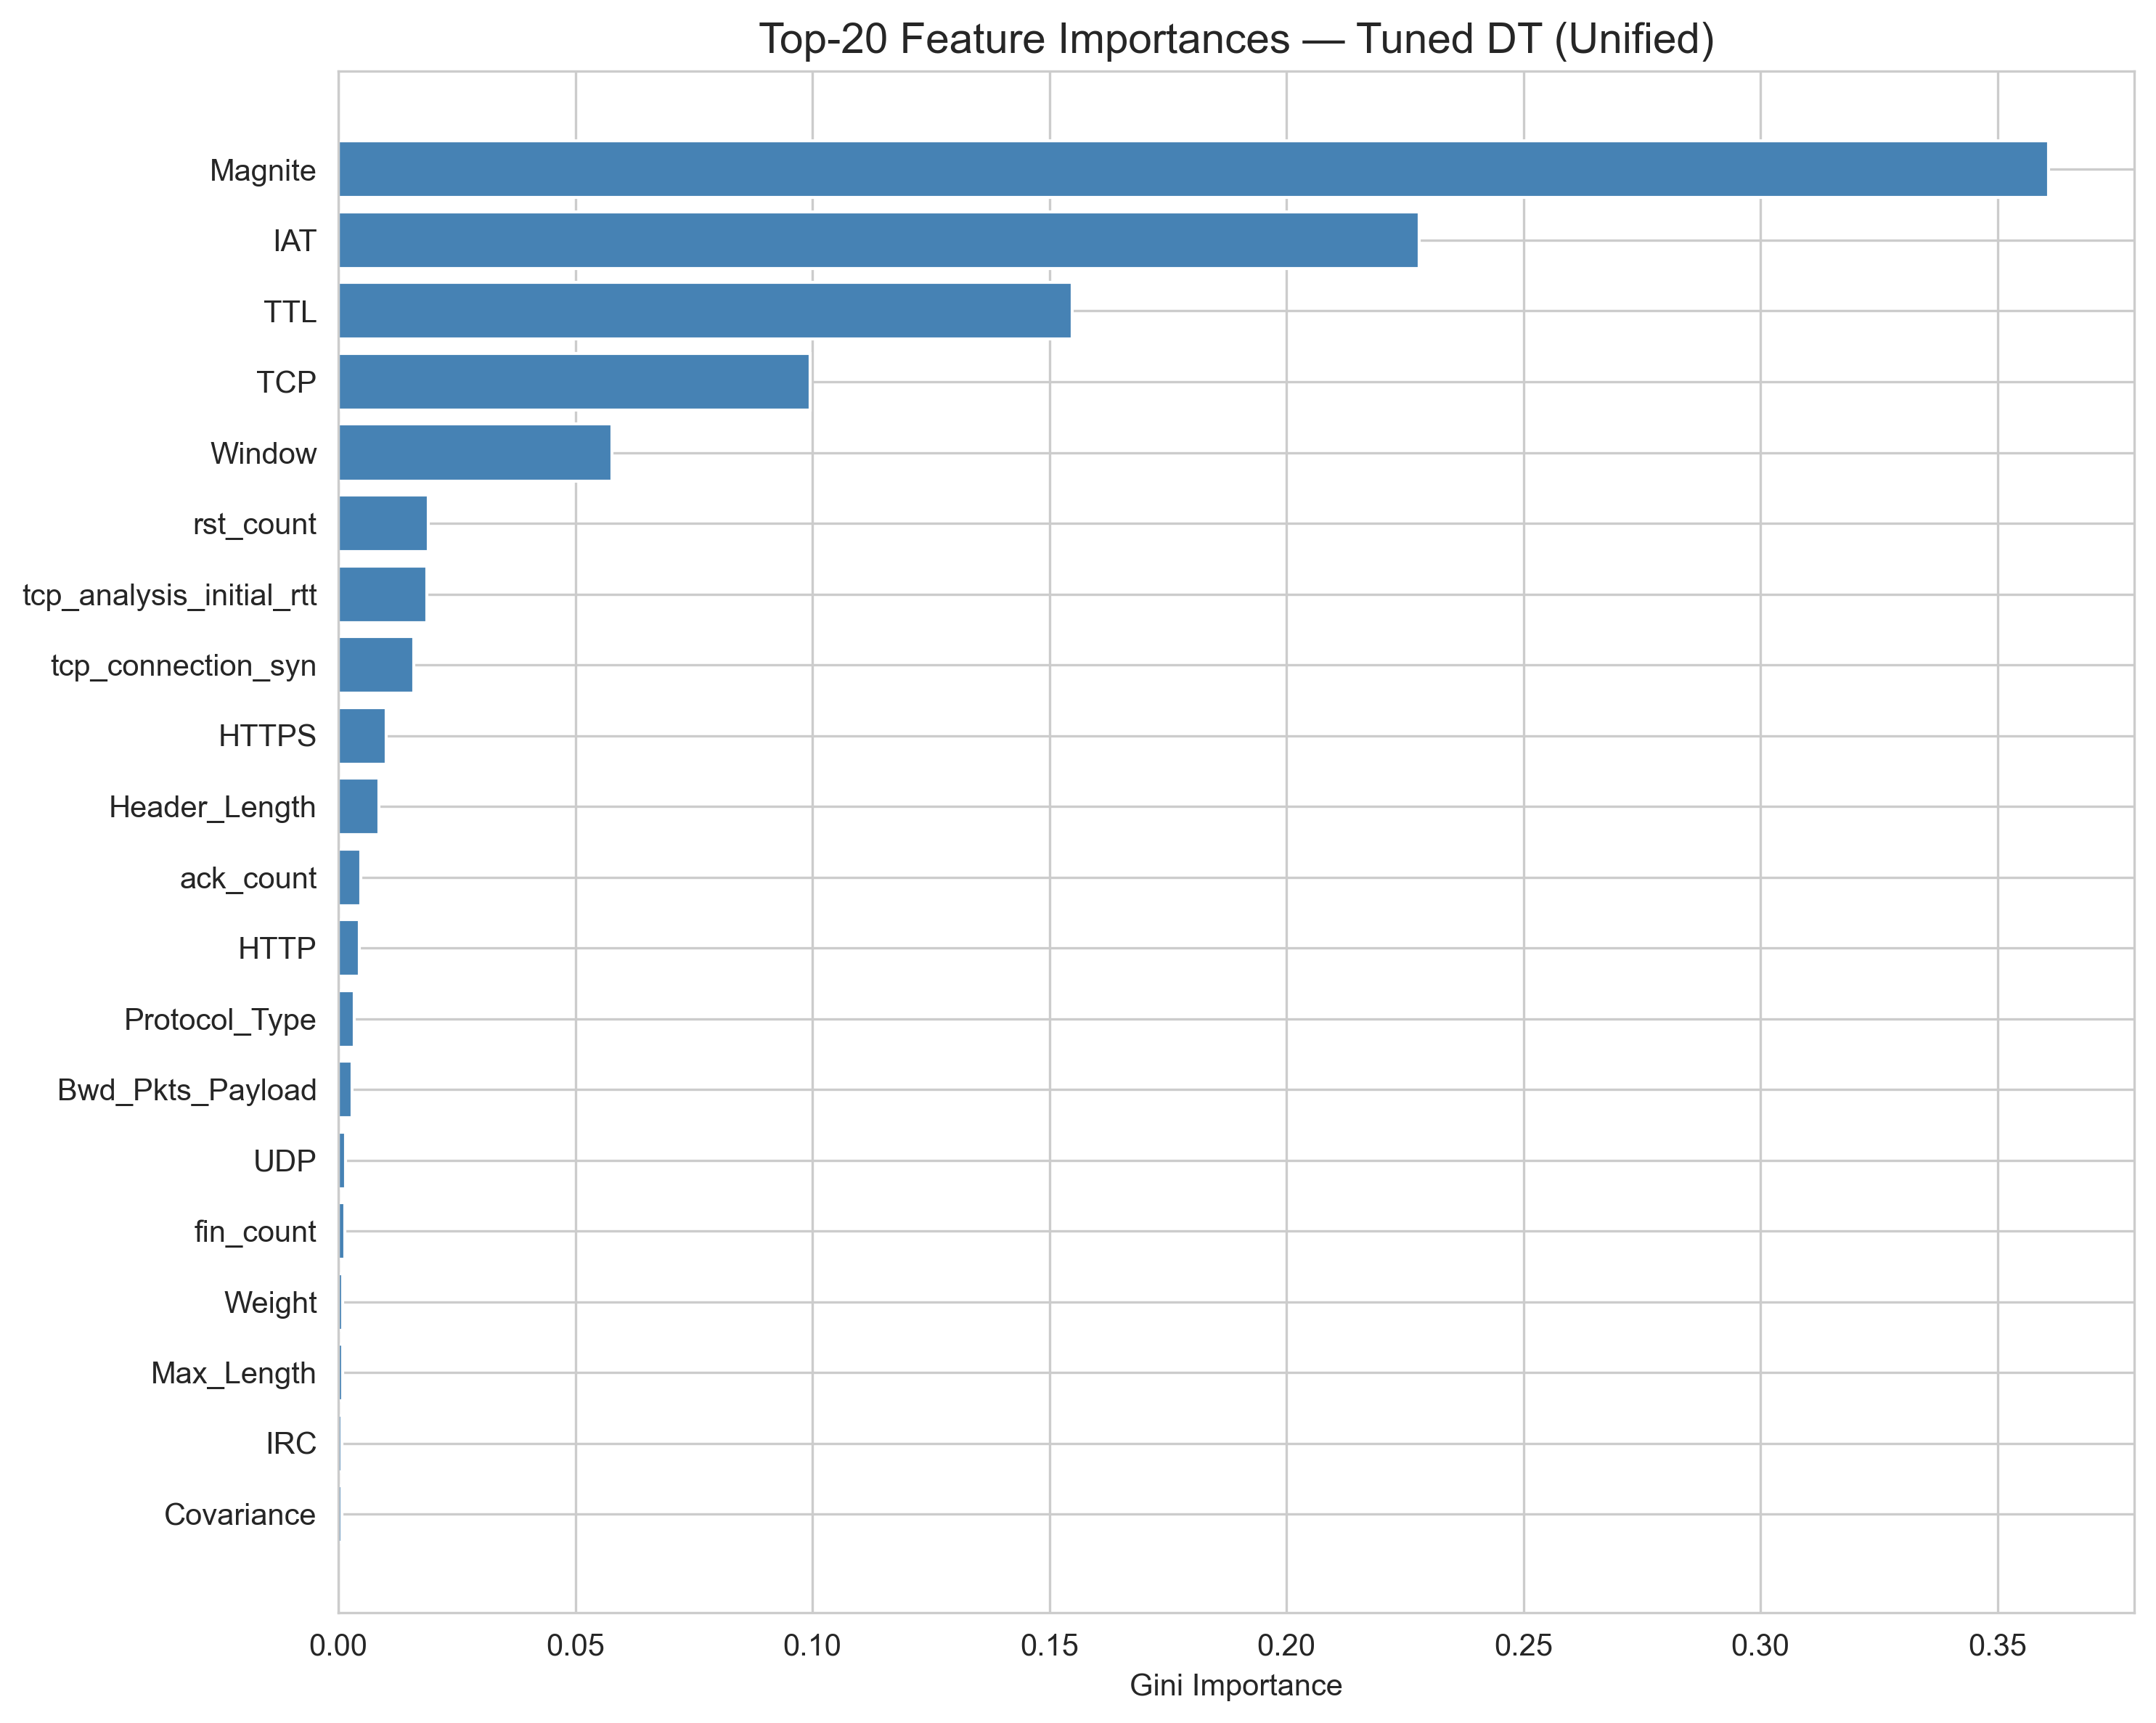
\includegraphics[width=0.85\textwidth]{ch5_dt_feature_importance_unified.png}
\caption{Top-20 feature importances for the tuned Decision Tree (Unified regime).}
\label{fig:dt-feature-importance}
\end{figure}

\begin{figure}[H]
\centering
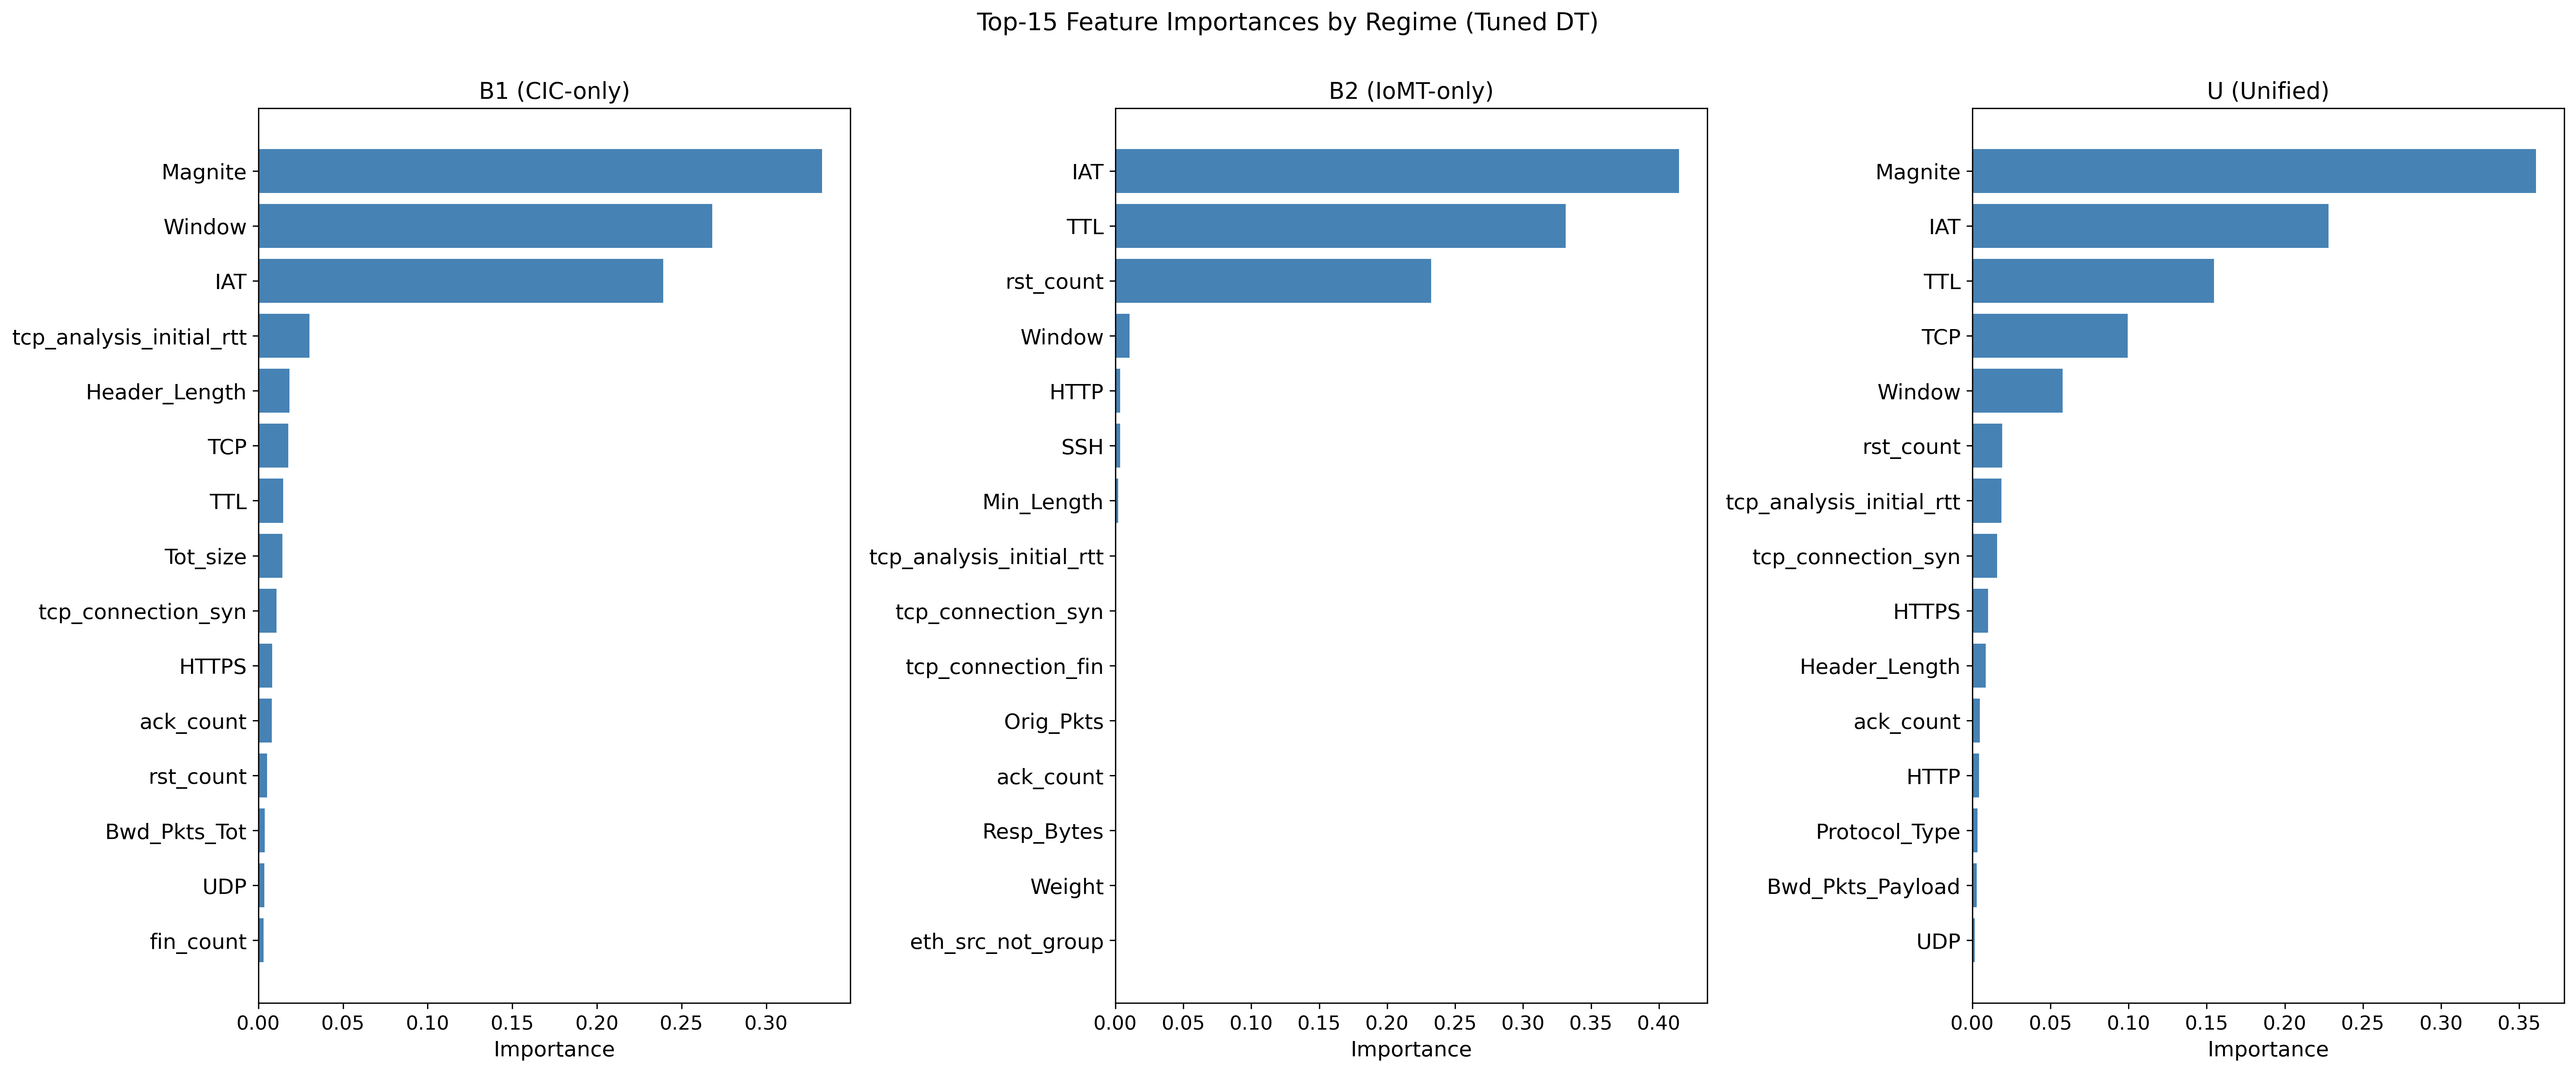
\includegraphics[width=\textwidth]{ch5_dt_feature_importance_comparison.png}
\caption{Feature importance comparison across the three training regimes (tuned DT, top-15).}
\label{fig:dt-fi-comparison}
\end{figure}

\subsubsection{Per-Class Analysis}

Figure~\ref{fig:dt-per-class-f1} breaks down F1-score by class for each tuned regime on the full test set. Table~\ref{tab:dt-perclass-unified} presents the detailed per-class metrics for the tuned unified model.

\begin{figure}[H]
\centering
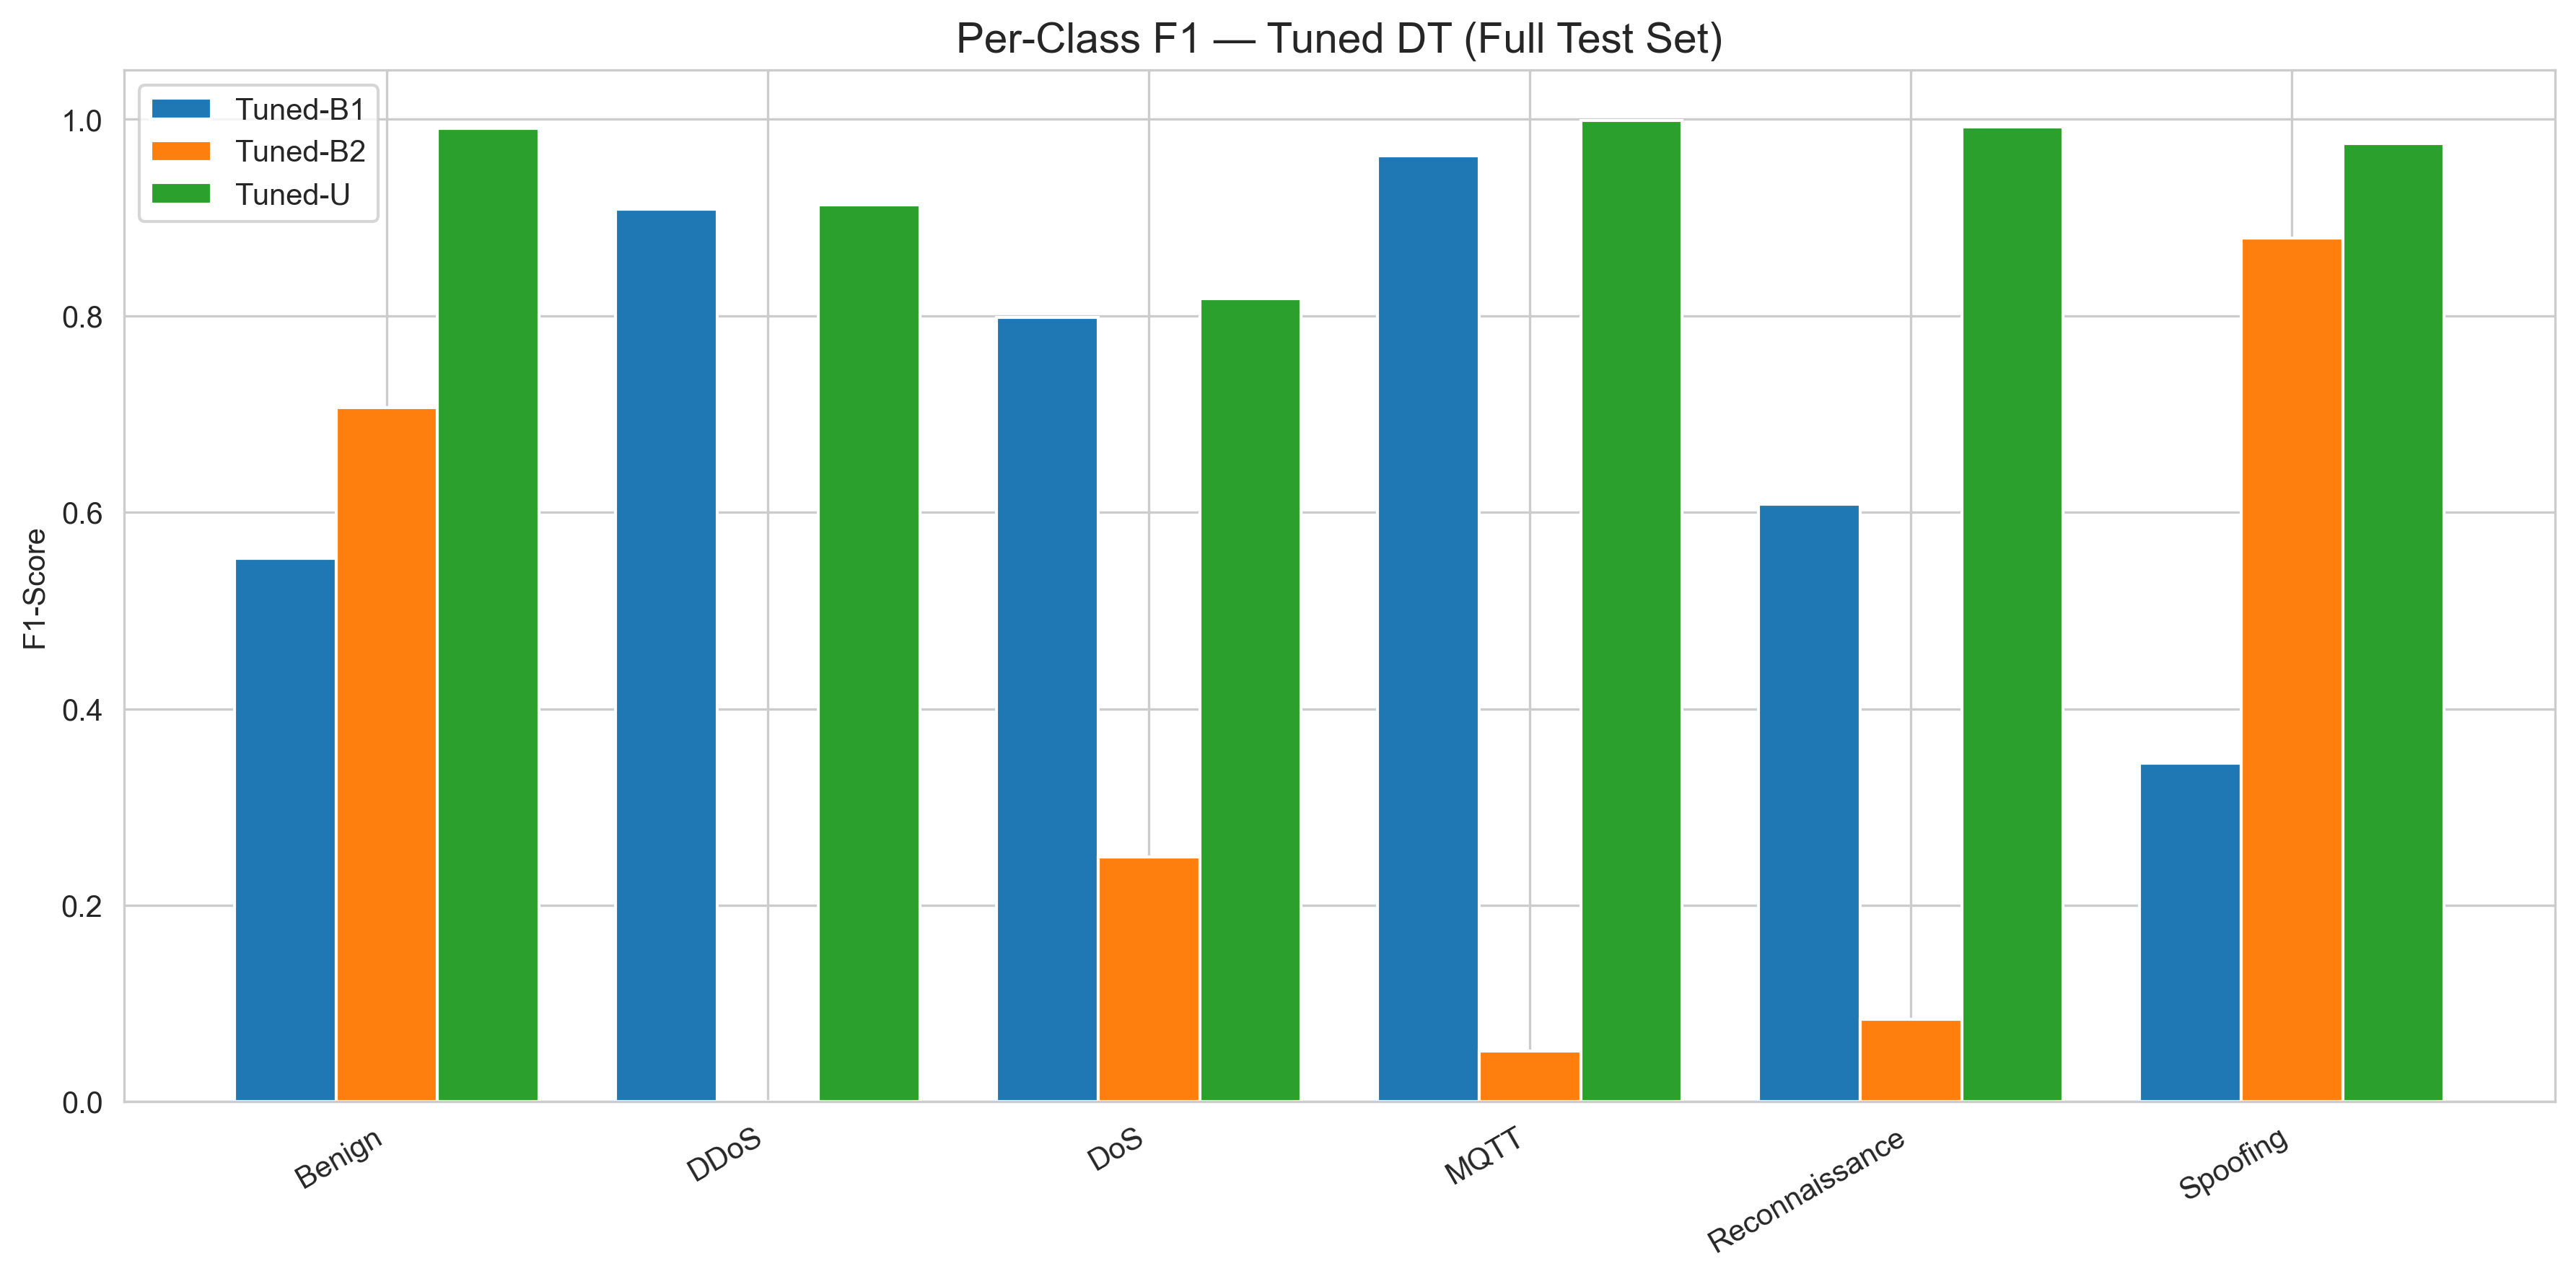
\includegraphics[width=0.85\textwidth]{ch5_dt_per_class_f1.png}
\caption{Per-class F1-score comparison across regimes (tuned DT, full test set).}
\label{fig:dt-per-class-f1}
\end{figure}

\begin{table}[H]
\centering
\caption{Per-class classification report for the tuned unified Decision Tree on the full test set (1,201,731 samples).}
\label{tab:dt-perclass-unified}
\small
\begin{tabular}{@{}l r r r r@{}}
\toprule
\textbf{Class} & \textbf{Precision} & \textbf{Recall} & \textbf{F1-Score} & \textbf{Support} \\
\midrule
Benign          & 0.99 & 1.00 & 0.99 &     8,018 \\
DDoS            & 0.97 & 0.86 & 0.91 &   805,244 \\
DoS             & 0.73 & 0.93 & 0.82 &   322,273 \\
MQTT            & 1.00 & 1.00 & 1.00 &    57,891 \\
Reconnaissance  & 0.99 & 0.99 & 0.99 &     6,904 \\
Spoofing        & 0.97 & 0.98 & 0.98 &     1,401 \\
\midrule
Accuracy        &      &      & 0.89 & 1,201,731 \\
Macro avg       & 0.94 & 0.96 & 0.95 & 1,201,731 \\
Weighted avg    & 0.91 & 0.89 & 0.89 & 1,201,731 \\
\bottomrule
\end{tabular}
\end{table}

The per-class results reveal a three-tier performance structure:

\paragraph{Tier 1 --- Near-perfect detection (F1 $\geq$ 0.98).}
MQTT (F1\,=\,1.00), Benign (0.99), Reconnaissance (0.99), and Spoofing (0.98) are classified with near-zero error. The MQTT class benefits from its distinct protocol-level features (MQTT-specific packet patterns). Benign and Reconnaissance traffic are also well-separated in the 58-feature space. Notably, Spoofing achieves F1\,=\,0.98 despite representing only 0.12\% of the test data (1,401 samples), confirming that the balanced class weights successfully compensated for extreme rarity. This success is also attributable to the distinctive network fingerprint of ARP Spoofing, which produces characteristic patterns in features such as \texttt{eth\_src\_not\_group} and \texttt{TTL}.

\paragraph{Tier 2 --- The DDoS/DoS confusion boundary.}
DDoS (F1\,=\,0.91) and DoS (F1\,=\,0.82) are the only classes with substantial error. Detailed inspection of the confusion matrix (Figure~\ref{fig:dt-confusion-unified}) reveals that 109,220 DDoS samples (13.6\%) are misclassified as DoS, and 24,020 DoS samples (7.5\%) are misclassified as DDoS. These 133,240 cross-confused samples account for \textbf{99.8\% of all classification errors} across the entire test set. This asymmetry manifests as:
\begin{itemize}[nosep]
  \item \textbf{DDoS}: High precision (0.97) but reduced recall (0.86) --- the model rarely labels a non-DDoS sample as DDoS, but misses 14\% of true DDoS traffic by labeling it DoS.
  \item \textbf{DoS}: High recall (0.93) but reduced precision (0.73) --- the model catches most DoS attacks, but also absorbs many DDoS samples as false positives.
\end{itemize}

This confusion is \textit{expected} and reflects a fundamental characteristic of the feature space: TCP/IP-based DDoS and DoS attacks (SYN floods, ICMP floods, UDP floods, TCP floods) share nearly identical per-window network statistics. The distinguishing factor---the number of attacking sources---is not directly captured by the 58 MIOTTA features, which aggregate flows within a time window without retaining source-level diversity information.

\paragraph{Accuracy vs.\ macro-F1 discrepancy.}
The overall accuracy (0.89) appears lower than the macro-F1 (0.95) because accuracy is dominated by the majority class: DDoS constitutes 67\% of the test data, and its recall of 0.86 drags down the global accuracy. In contrast, macro-F1 gives equal weight to each class, thereby reflecting the excellent performance on all four minority classes. For IDS evaluation on imbalanced datasets, macro-F1 is the more informative metric, as discussed in Section~\ref{subsec:experimental-setup}.

\subsubsection{Summary}

The Decision Tree experiments establish clear empirical evidence regarding the benefit of multi-source integration:

\begin{itemize}[nosep]
  \item \textbf{Single-source models fail cross-domain.} B1 achieves macro-F1 = 0.9226 in-domain but only 0.2474 on IoMT data. B2 achieves 0.8332 in-domain but collapses to 0.0523 on CIC data---unable to recognize DDoS traffic it has never seen.
  \item \textbf{Unified training resolves the gap.} The tuned unified DT achieves macro-F1 = 0.9480 on the full test set, outperforming both baselines on every cross-domain slice. This is a +25.2 percentage-point absolute improvement (or +36.2\% relative) over the best single-source model (B1) on the full test.
  \item \textbf{Tuning yields modest gains.} Hyperparameter tuning improved all three regimes: B1 (+2.8\%), B2 (--0.3\%), U (+1.1\%) on their respective full-test macro-F1. The selected hyperparameters favor shallower trees (\texttt{max\_depth}=15) with entropy criterion, reducing overfitting compared to the unlimited-depth baseline.
  \item \textbf{Class-level analysis.} Four of six categories (Benign, MQTT, Reconnaissance, Spoofing) achieve F1 $\geq$ 0.98, confirming that balanced class weights effectively address extreme imbalance. The only significant weakness is the DDoS/DoS confusion boundary (133,240 cross-misclassified samples, 99.8\% of all errors), attributable to the inherent similarity of these attack families at the network-feature level. Ensemble methods (RF, XGBoost) are expected to improve this boundary through their capacity for more nuanced decision boundaries.
\end{itemize}

Detailed discussion of these results, in the context of the other classifiers and the research question, is deferred to Section~\ref{subsec:discussion}.

\subsection{Random Forest Classifier}
\label{subsec:random-forest}

The Random Forest (RF) extends the Decision Tree with bagging and feature randomization, averaging predictions over an ensemble of decorrelated trees. The same three-regime protocol applies: baseline (100 trees, balanced class weights) followed by tuned models from \texttt{RandomizedSearchCV} (50 iterations, 3-fold CV, macro-F1 scoring), with the subsample-then-full-refit procedure described above for computational feasibility.

\subsubsection{Baseline Results}

Table~\ref{tab:rf-baseline} reports baseline RF performance. Patterns mirror the Decision Tree: single-source models achieve strong in-domain scores but degrade sharply on the opposite source's test slice.

\begin{table}[H]
\centering
\caption{Baseline Random Forest (100 trees, balanced class weights) evaluation matrix.}
\label{tab:rf-baseline}
\small
\begin{tabular}{@{}l l c c c@{}}
\toprule
\textbf{Regime} & \textbf{Test slice} & \textbf{Macro-F1} & \textbf{Weighted-F1} & \textbf{Accuracy} \\
\midrule
B1 (CIC-only) & CIC (in-domain)  & 0.9175 & 0.8744 & 0.8743 \\
B1 (CIC-only) & IoMT (cross)     & 0.1982 & 0.3601 & 0.3903 \\
B1 (CIC-only) & Full             & 0.6677 & 0.8615 & 0.8631 \\
\midrule
B2 (IoMT-only) & IoMT (in-domain) & 0.8333 & 1.0000 & 1.0000 \\
B2 (IoMT-only) & CIC (cross)      & 0.1570 & 0.1226 & 0.2420 \\
B2 (IoMT-only) & Full             & 0.2945 & 0.1350 & 0.2594 \\
\midrule
U (Unified)    & CIC              & 0.9178 & 0.8744 & 0.8743 \\
U (Unified)    & IoMT             & 0.8330 & 0.9996 & 0.9996 \\
U (Unified)    & Full             & \textbf{0.9404} & 0.8772 & 0.8771 \\
\bottomrule
\end{tabular}
\end{table}

\subsubsection{Tuned Results}

Table~\ref{tab:rf-tuned} reports tuned RF results. Table~\ref{tab:rf-best-params} lists the selected hyperparameters and cross-validated macro-F1 on the search subsample (or full training set for B2).

\begin{table}[H]
\centering
\caption{Tuned Random Forest evaluation matrix.}
\label{tab:rf-tuned}
\small
\begin{tabular}{@{}l l c c c@{}}
\toprule
\textbf{Regime} & \textbf{Test slice} & \textbf{Macro-F1} & \textbf{Weighted-F1} & \textbf{Accuracy} \\
\midrule
Tuned B1 & CIC (in-domain)  & 0.9149 & 0.8903 & 0.8866 \\
Tuned B1 & IoMT (cross)     & 0.3423 & 0.5013 & 0.5089 \\
Tuned B1 & Full             & 0.7395 & 0.8811 & 0.8779 \\
\midrule
Tuned B2 & IoMT (in-domain) & 0.8333 & 1.0000 & 1.0000 \\
Tuned B2 & CIC (cross)      & 0.0586 & 0.0537 & 0.0707 \\
Tuned B2 & Full             & 0.2029 & 0.0680 & 0.0921 \\
\midrule
Tuned U  & CIC              & 0.9285 & 0.8895 & 0.8858 \\
Tuned U  & IoMT             & 0.8329 & 0.9995 & 0.9995 \\
Tuned U  & Full             & \textbf{0.9487} & 0.8919 & 0.8884 \\
\bottomrule
\end{tabular}
\end{table}

\paragraph{Note on Macro-F1 (IoMT slice, Tuned U).}
The IoMT-only test slice contains no DDoS samples; accordingly, the global six-class Macro-F1 reported for the Random Forest on that slice (0.8329) averages over a zero-score DDoS column, following the same convention as the Decision Tree table. Weighted-F1 and accuracy remain near-perfect on the same slice because those metrics are support-weighted and are not penalized by an absent class.

\begin{table}[H]
\centering
\caption{Best hyperparameters per regime (Random Forest, 50-iteration RandomizedSearchCV). CV F1m is the best cross-validated macro-F1 on the training fold used during search.}
\label{tab:rf-best-params}
\small
\begin{tabular}{@{}l c c c c c c c@{}}
\toprule
\textbf{Regime} & \textbf{trees} & \textbf{depth} & \textbf{mss} & \textbf{msl} & \textbf{max\_feat.} & \textbf{max\_samp.} & \textbf{CV F1m} \\
\midrule
B1 (CIC-only)  & 200 & 15 & 5 & 1 & 0.5 & 0.8 & 0.9024 \\
B2 (IoMT-only) & 300 & 15 & 5 & 1 & 0.3 & 0.8 & 0.9999 \\
U (Unified)    & 200 & 15 & 5 & 1 & 0.5 & 0.8 & 0.9390 \\
\bottomrule
\end{tabular}
\end{table}

\noindent\textit{Class weight:} B1 and U use \texttt{balanced}; B2 uses \texttt{balanced\_subsample}. All three regimes selected \texttt{max\_depth}=15 and \texttt{max\_samples}=0.8, indicating a preference for moderately deep trees with row subsampling per tree---a configuration that limits variance and memory footprint relative to unrestricted depth and full bootstrap samples.

\subsubsection{Cross-Domain Analysis}

Figure~\ref{fig:rf-confusion-unified} shows the normalized confusion matrix for the tuned unified RF on the full test set. Figure~\ref{fig:rf-cm-xd} shows the cross-domain matrices for B1$\to$IoMT and B2$\to$CIC.

\begin{figure}[H]
\centering
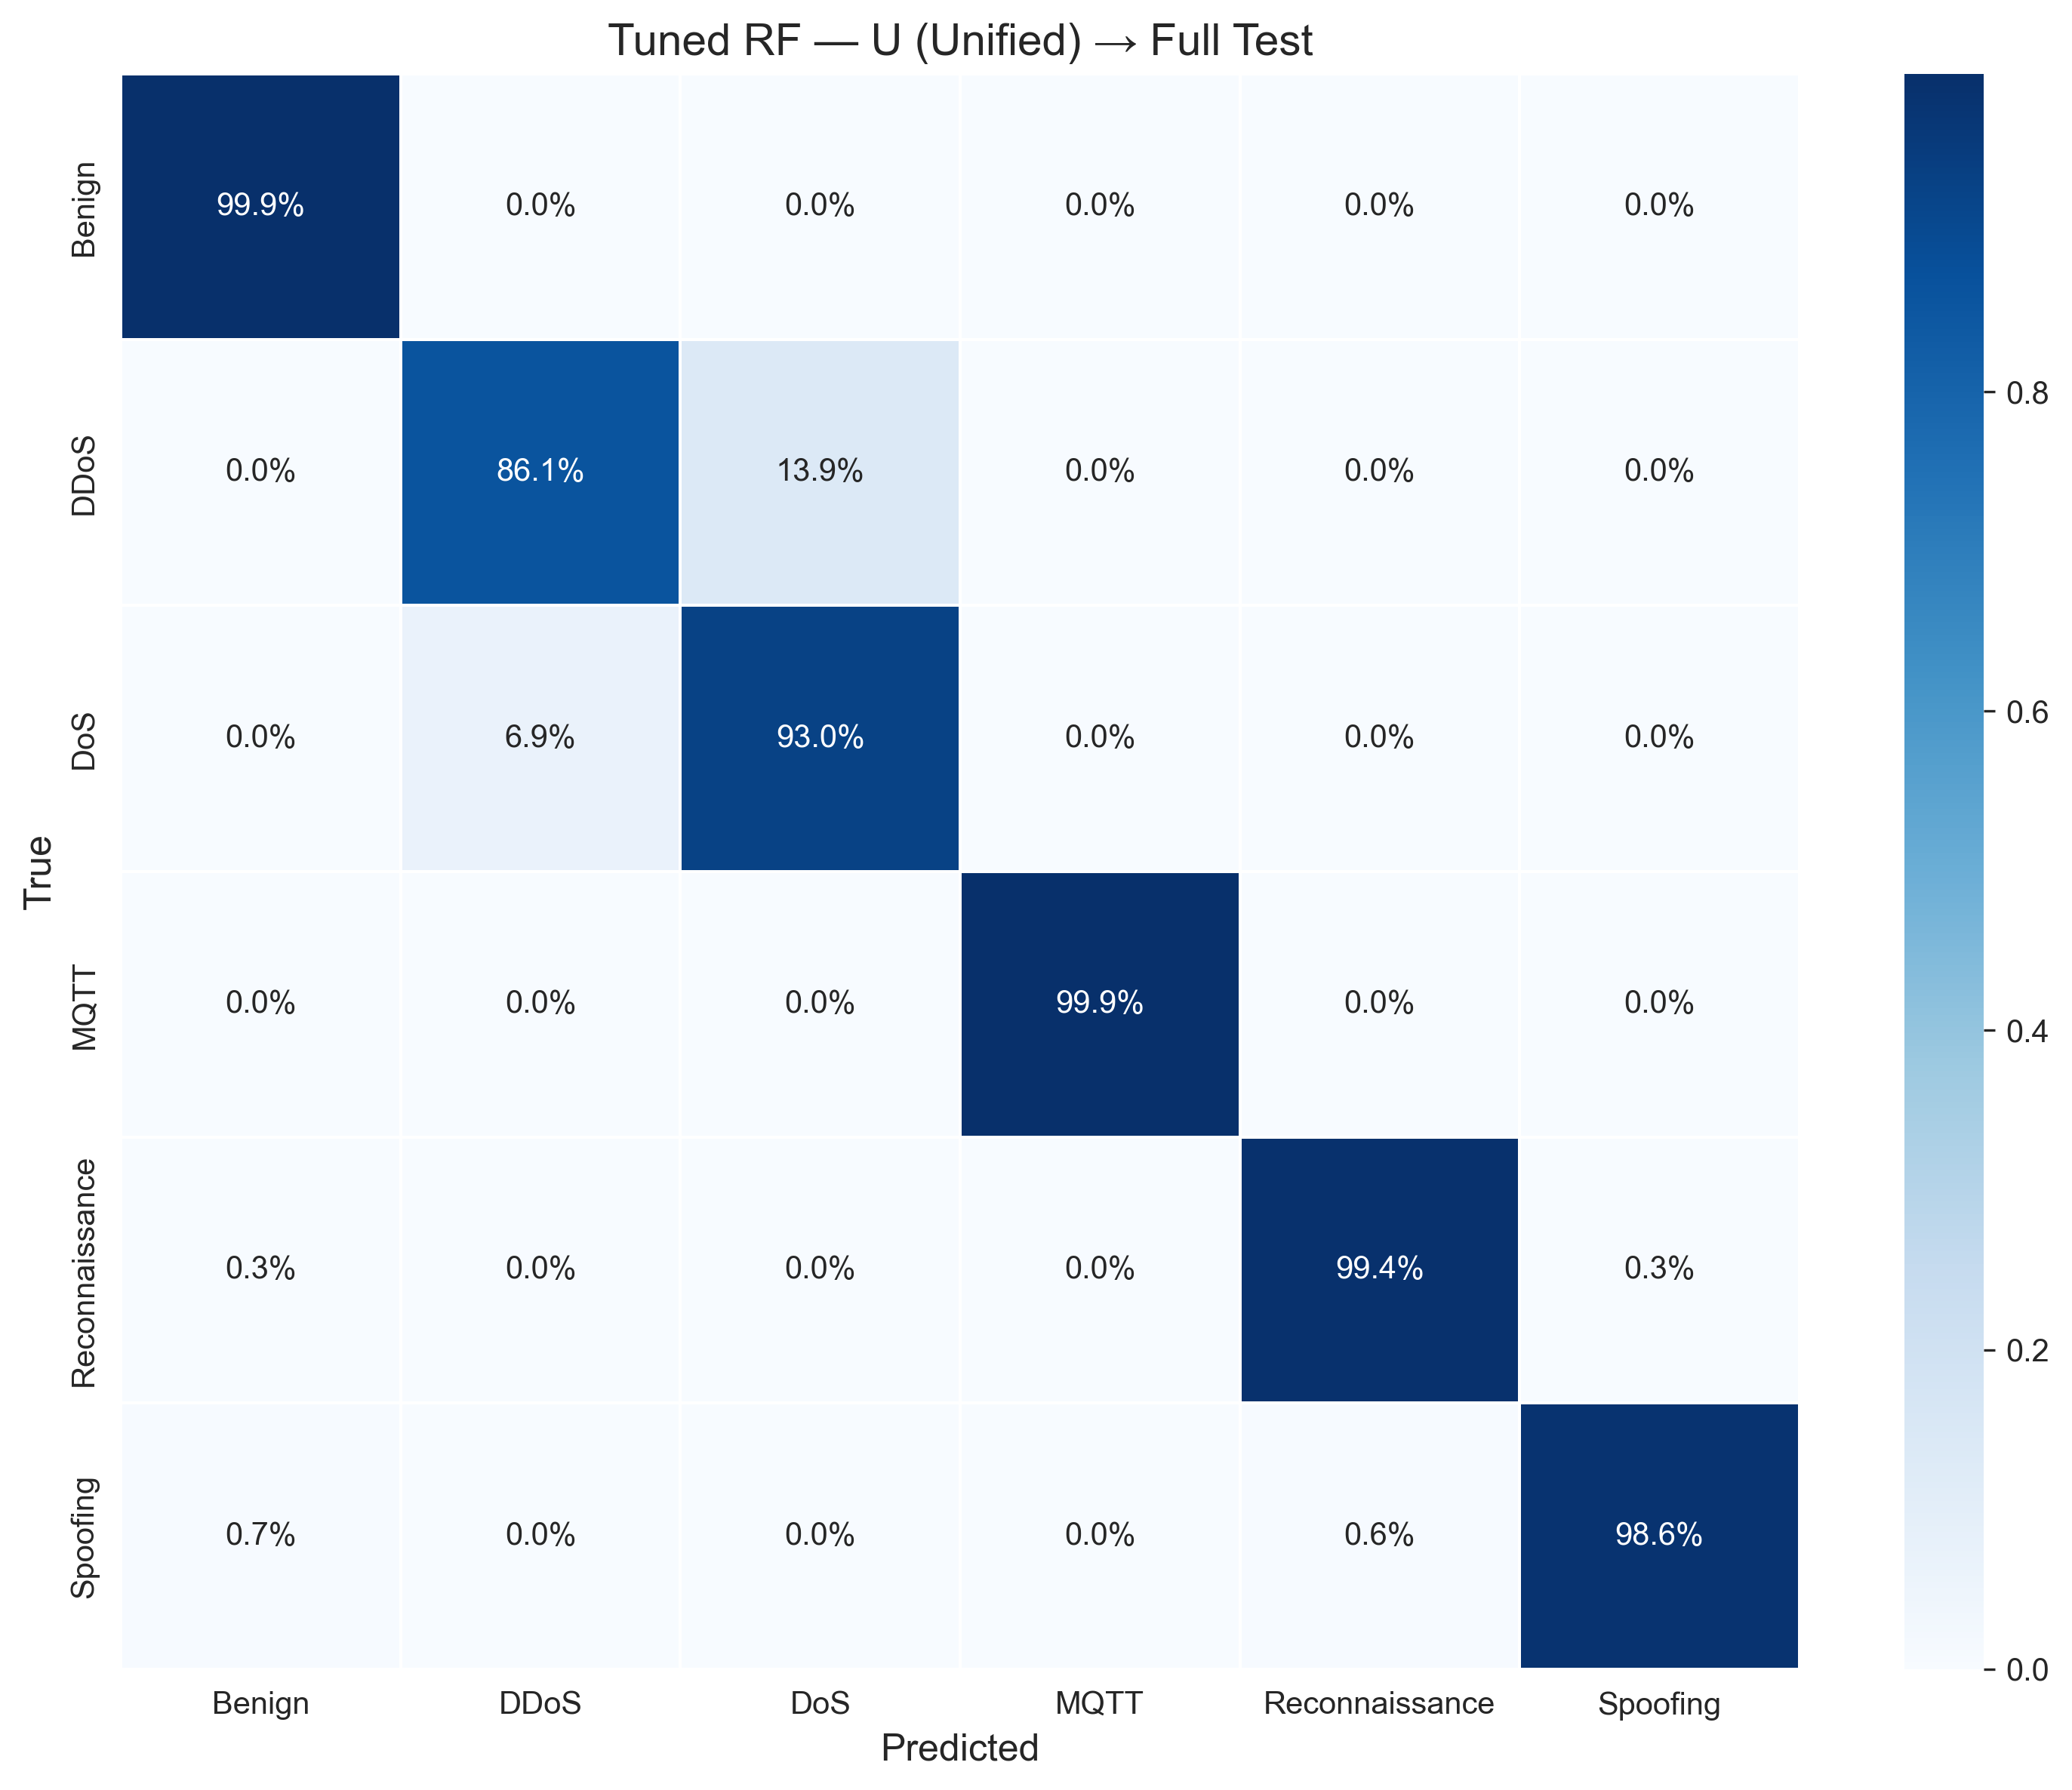
\includegraphics[width=0.75\textwidth]{ch5_rf_cm_u_full.png}
\caption{Normalized confusion matrix --- Tuned RF (Unified) on the full test set.}
\label{fig:rf-confusion-unified}
\end{figure}

\begin{figure}[H]
\centering
\begin{subfigure}[b]{0.48\textwidth}
  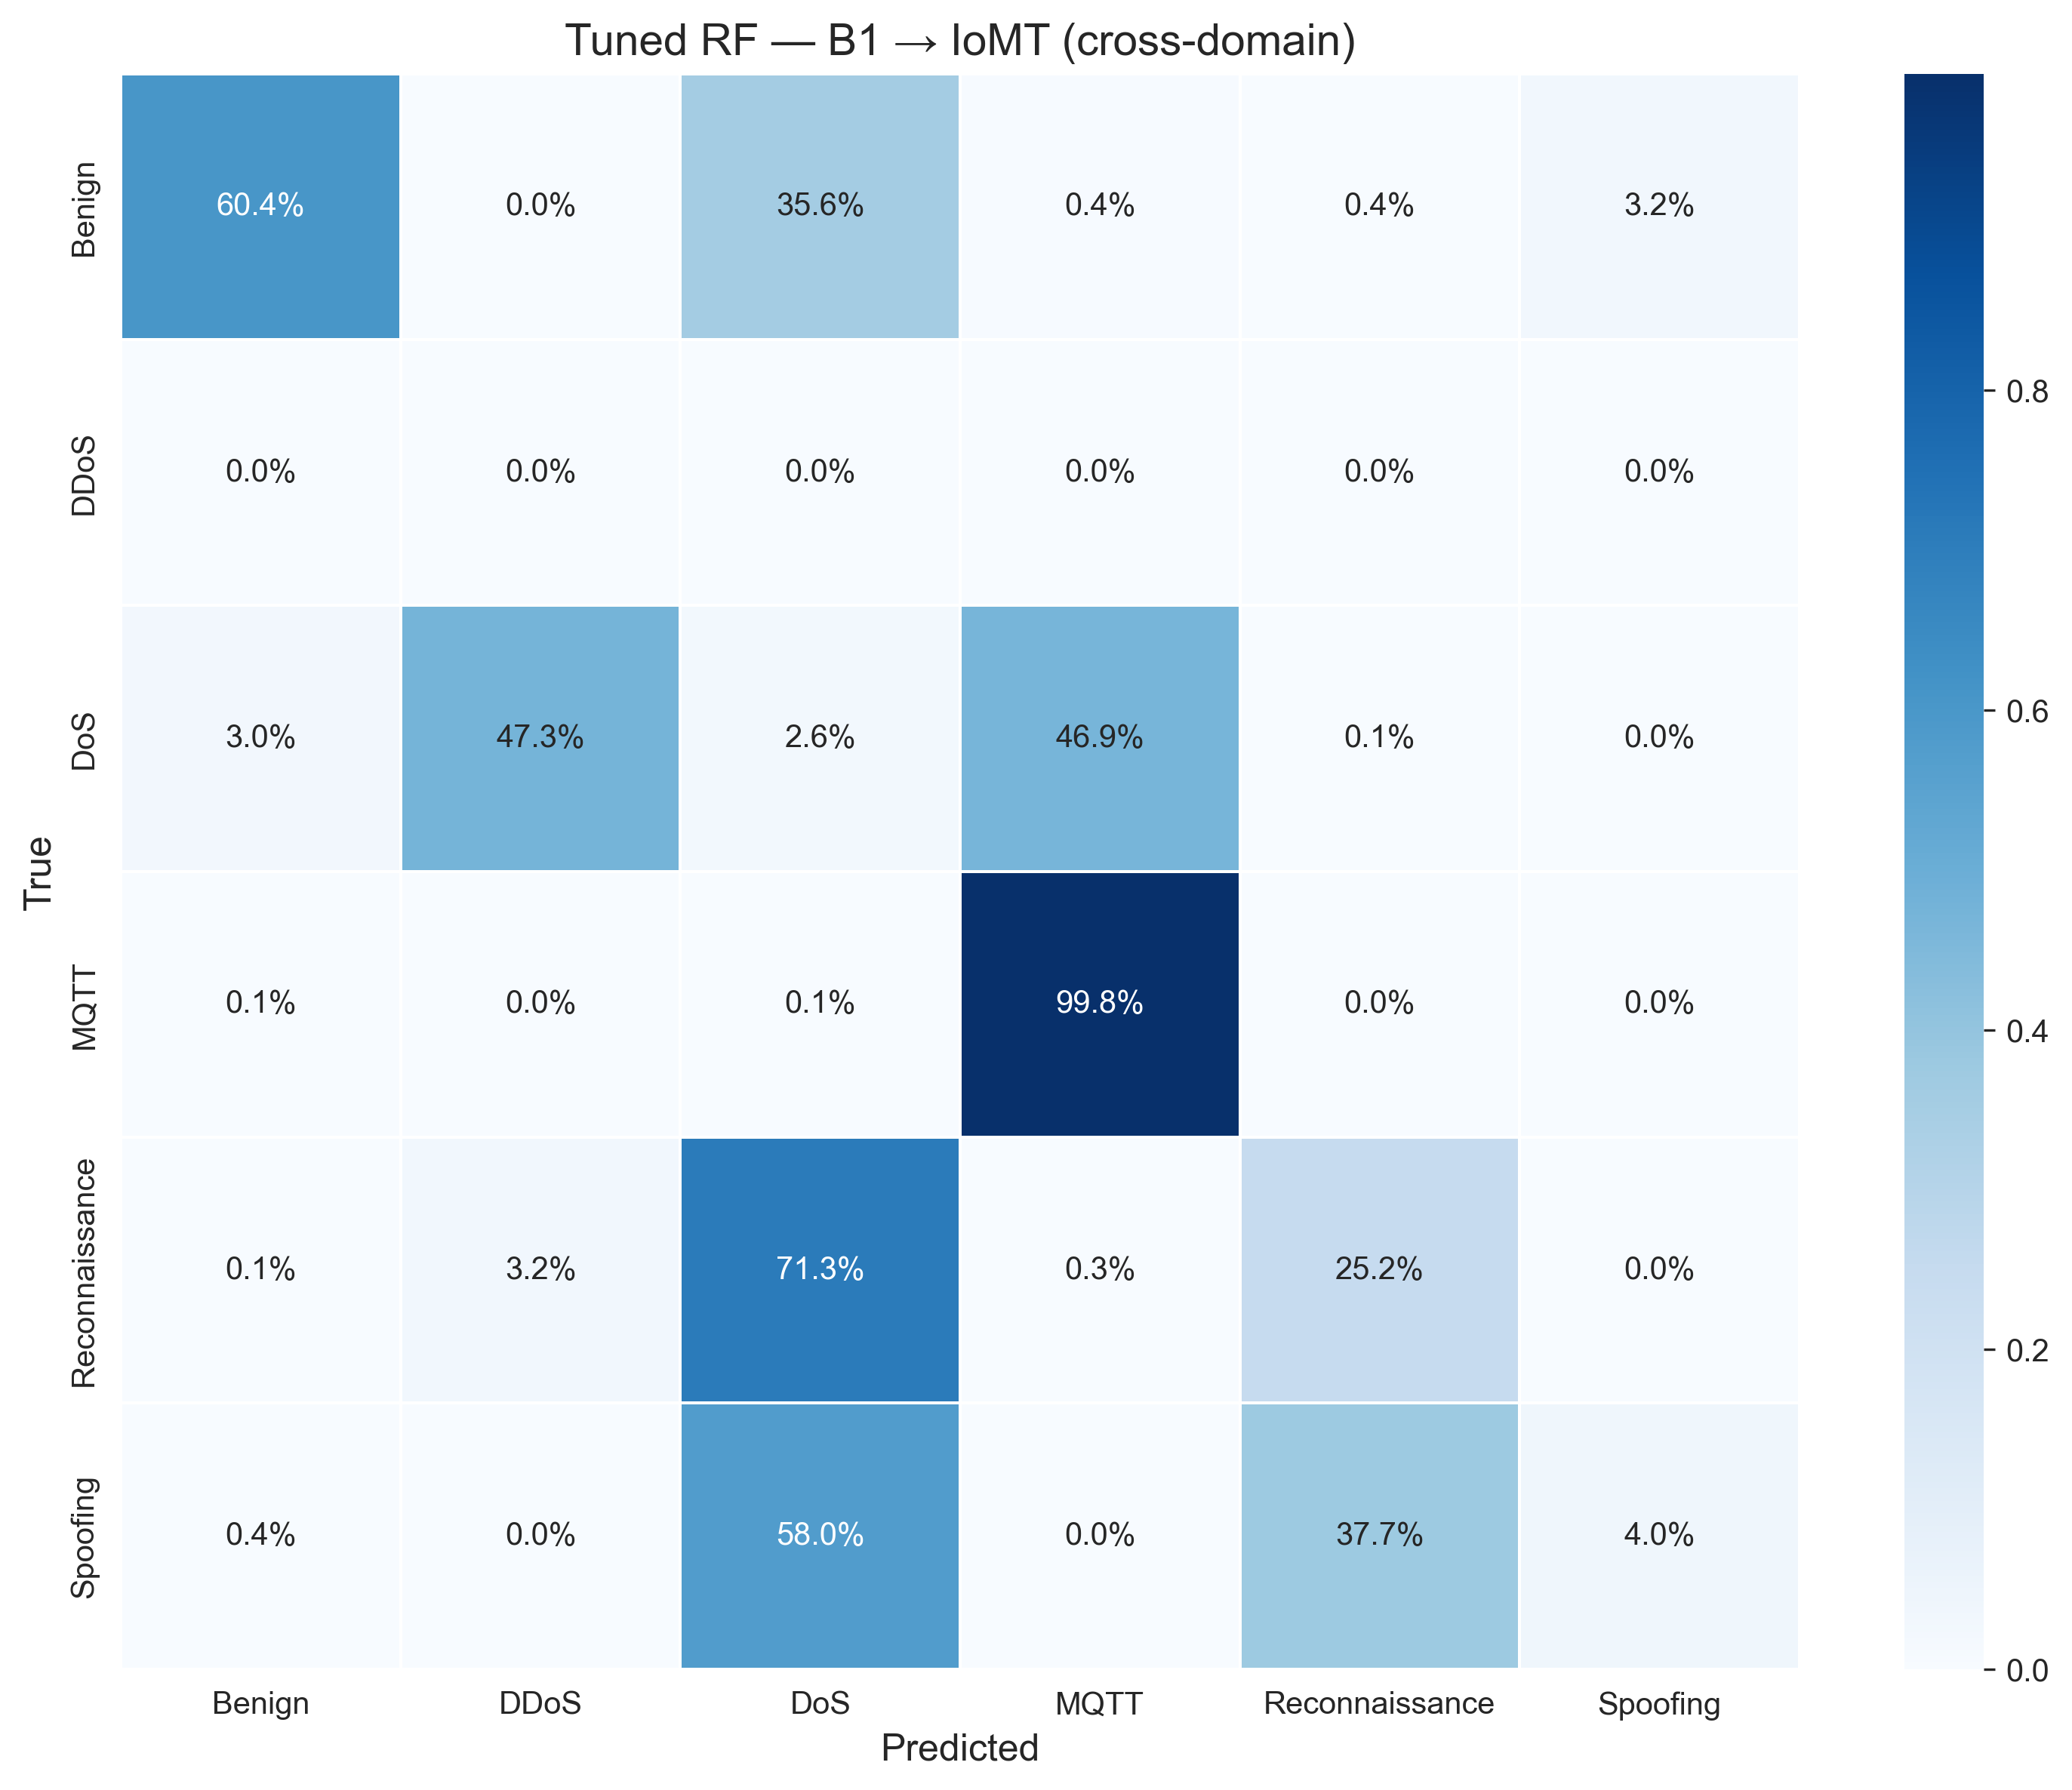
\includegraphics[width=\textwidth]{ch5_rf_cm_b1_xd_iomt.png}
  \caption{B1 (CIC-only) $\to$ IoMT test}
\end{subfigure}
\hfill
\begin{subfigure}[b]{0.48\textwidth}
  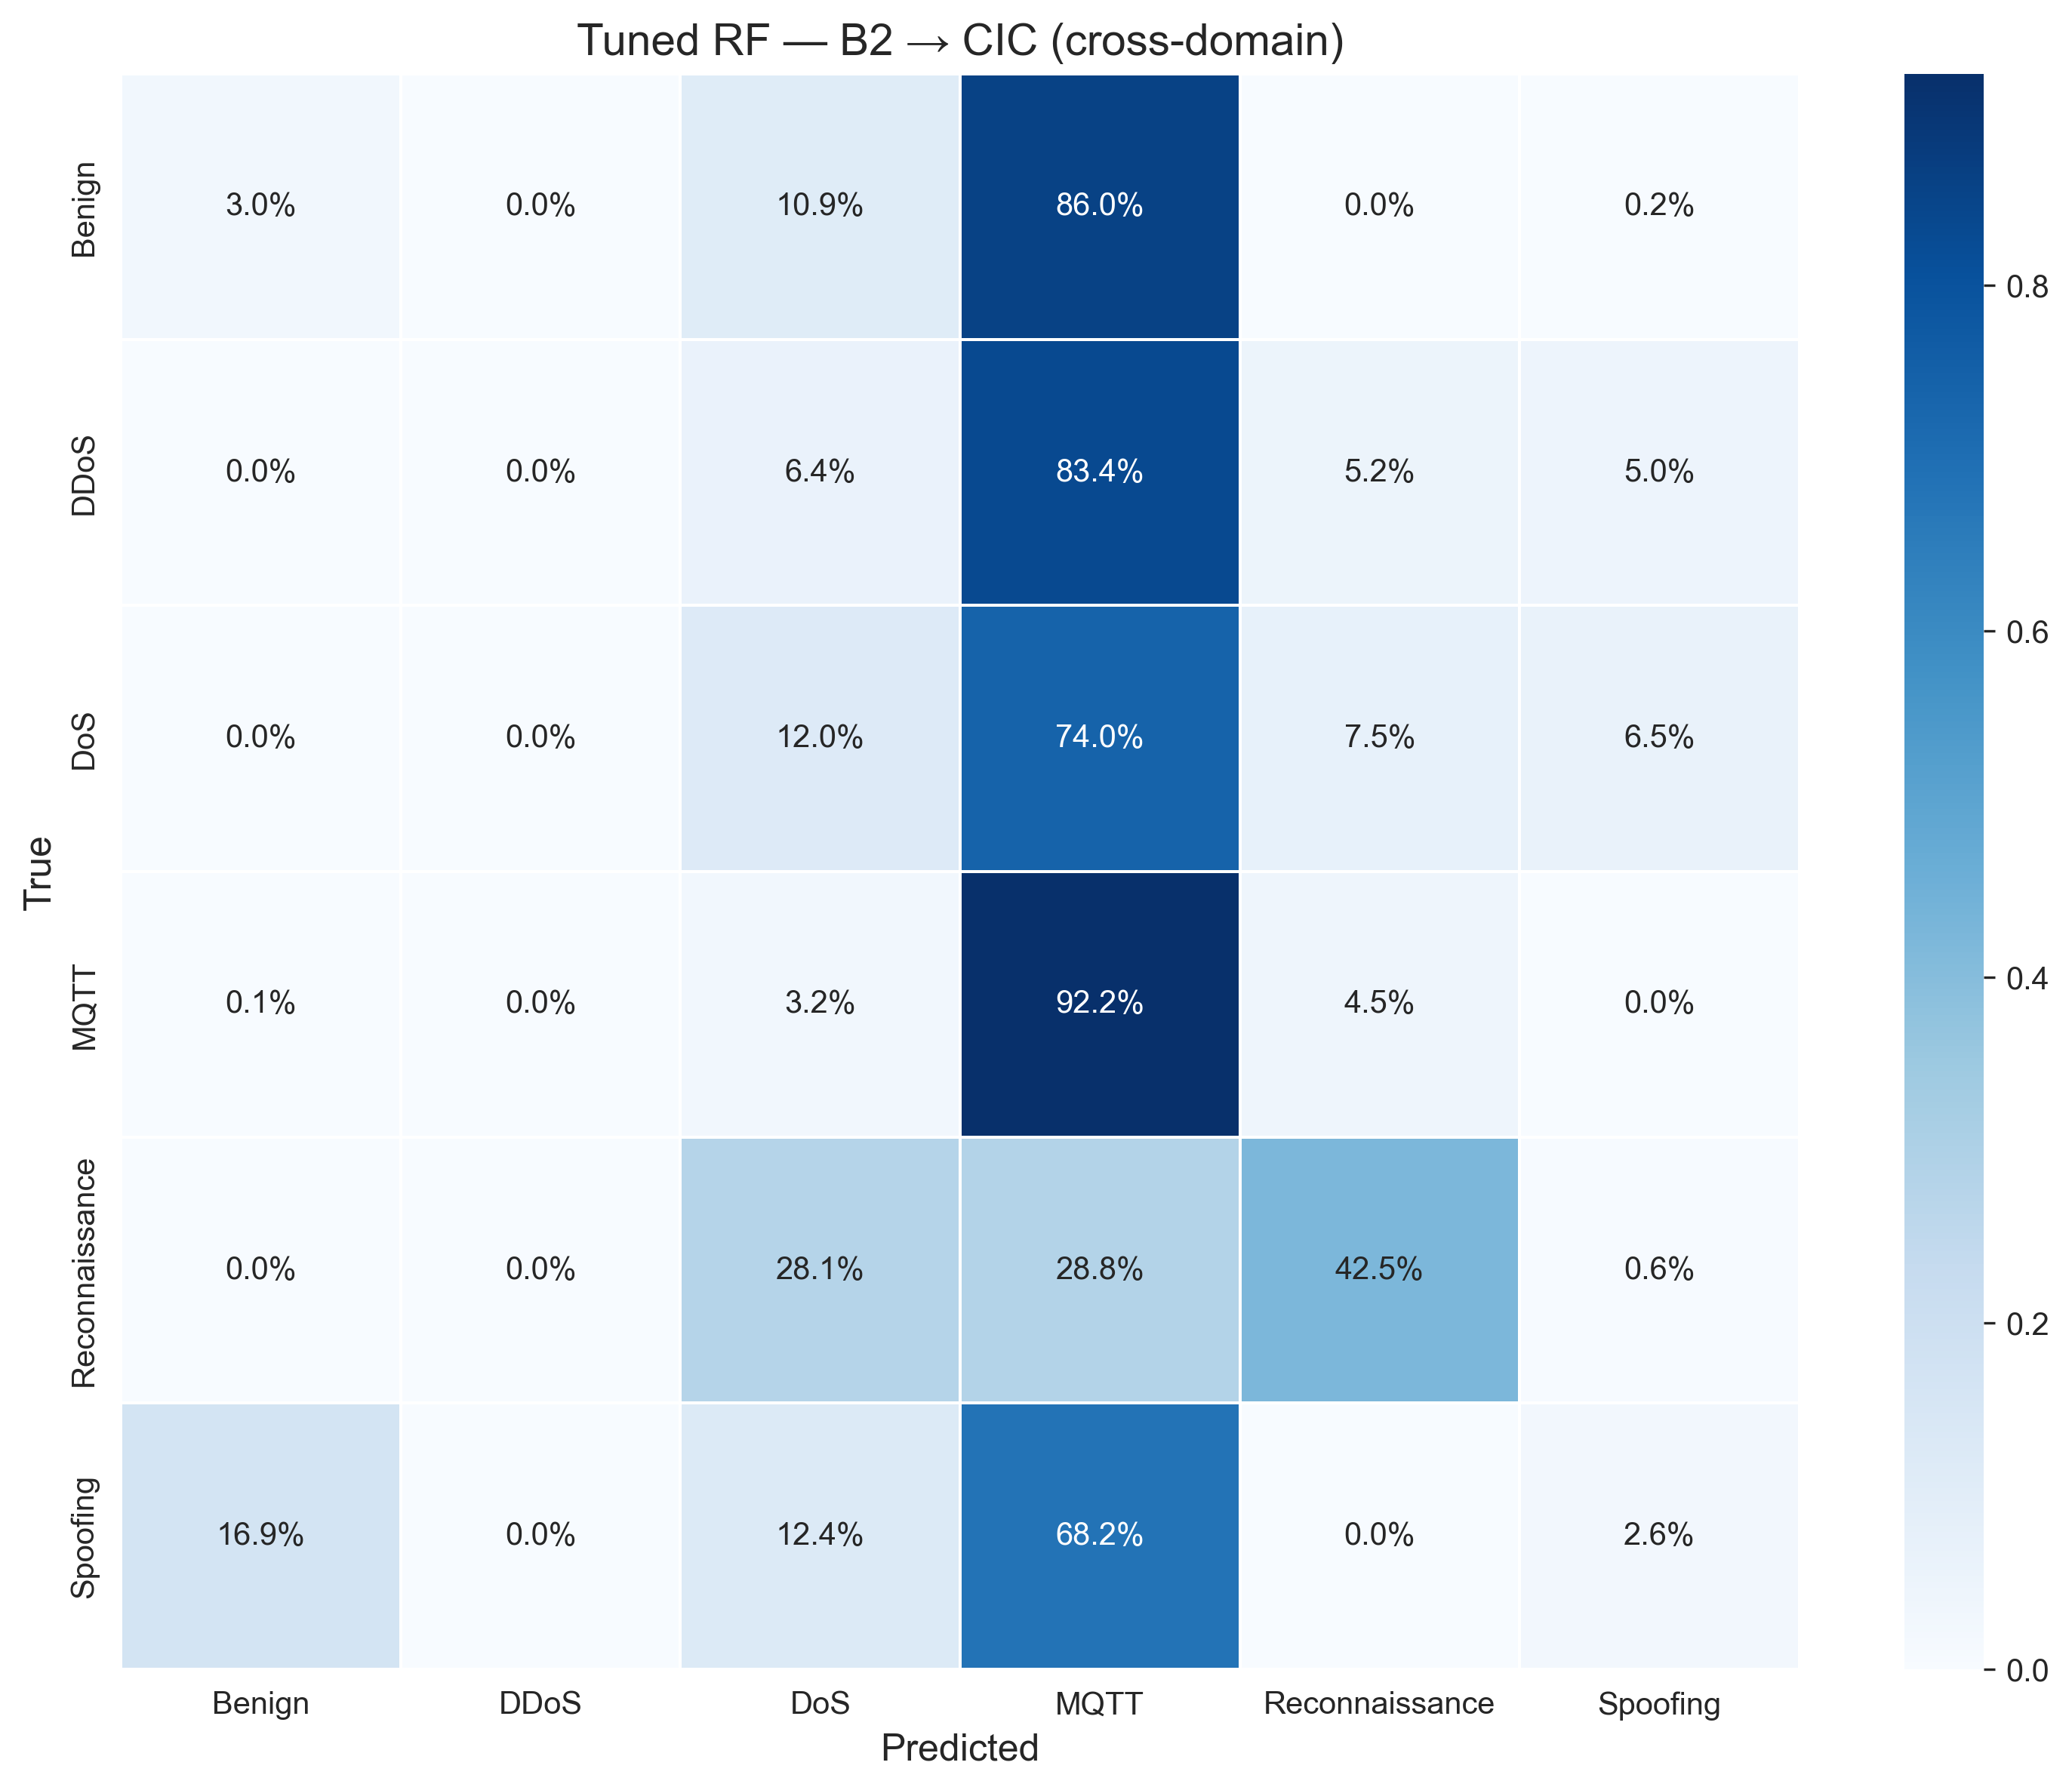
\includegraphics[width=\textwidth]{ch5_rf_cm_b2_xd_cic.png}
  \caption{B2 (IoMT-only) $\to$ CIC test}
\end{subfigure}
\caption{Cross-domain confusion matrices for tuned Random Forest models.}
\label{fig:rf-cm-xd}
\end{figure}

The unified RF confusion matrix (Figure~\ref{fig:rf-confusion-unified}) closely mirrors its Decision Tree counterpart: the dominant off-diagonal mass remains the bidirectional DDoS$\leftrightarrow$DoS confusion, while all other class pairs produce near-zero error. In the cross-domain scenario, the B1$\to$IoMT Macro-F1 (0.3423) is noticeably stronger than the equivalent DT score (0.2474), which suggests that bagging's variance reduction allows the ensemble to partially generalize CIC-trained feature patterns to the unseen IoMT distribution. The B2$\to$CIC result remains near-zero (0.0586) for the same structural reason as the Decision Tree: the IoMT-only model has never observed DDoS traffic, which constitutes the majority class of the CIC test slice, so the model cannot produce meaningful predictions on that slice regardless of its within-domain quality.

\subsubsection{Feature Importance}

Figure~\ref{fig:rf-feature-importance} and Figure~\ref{fig:rf-fi-comparison} show Gini-based importances for the tuned unified RF and a regime-wise comparison (top-15), respectively.

\begin{figure}[H]
\centering
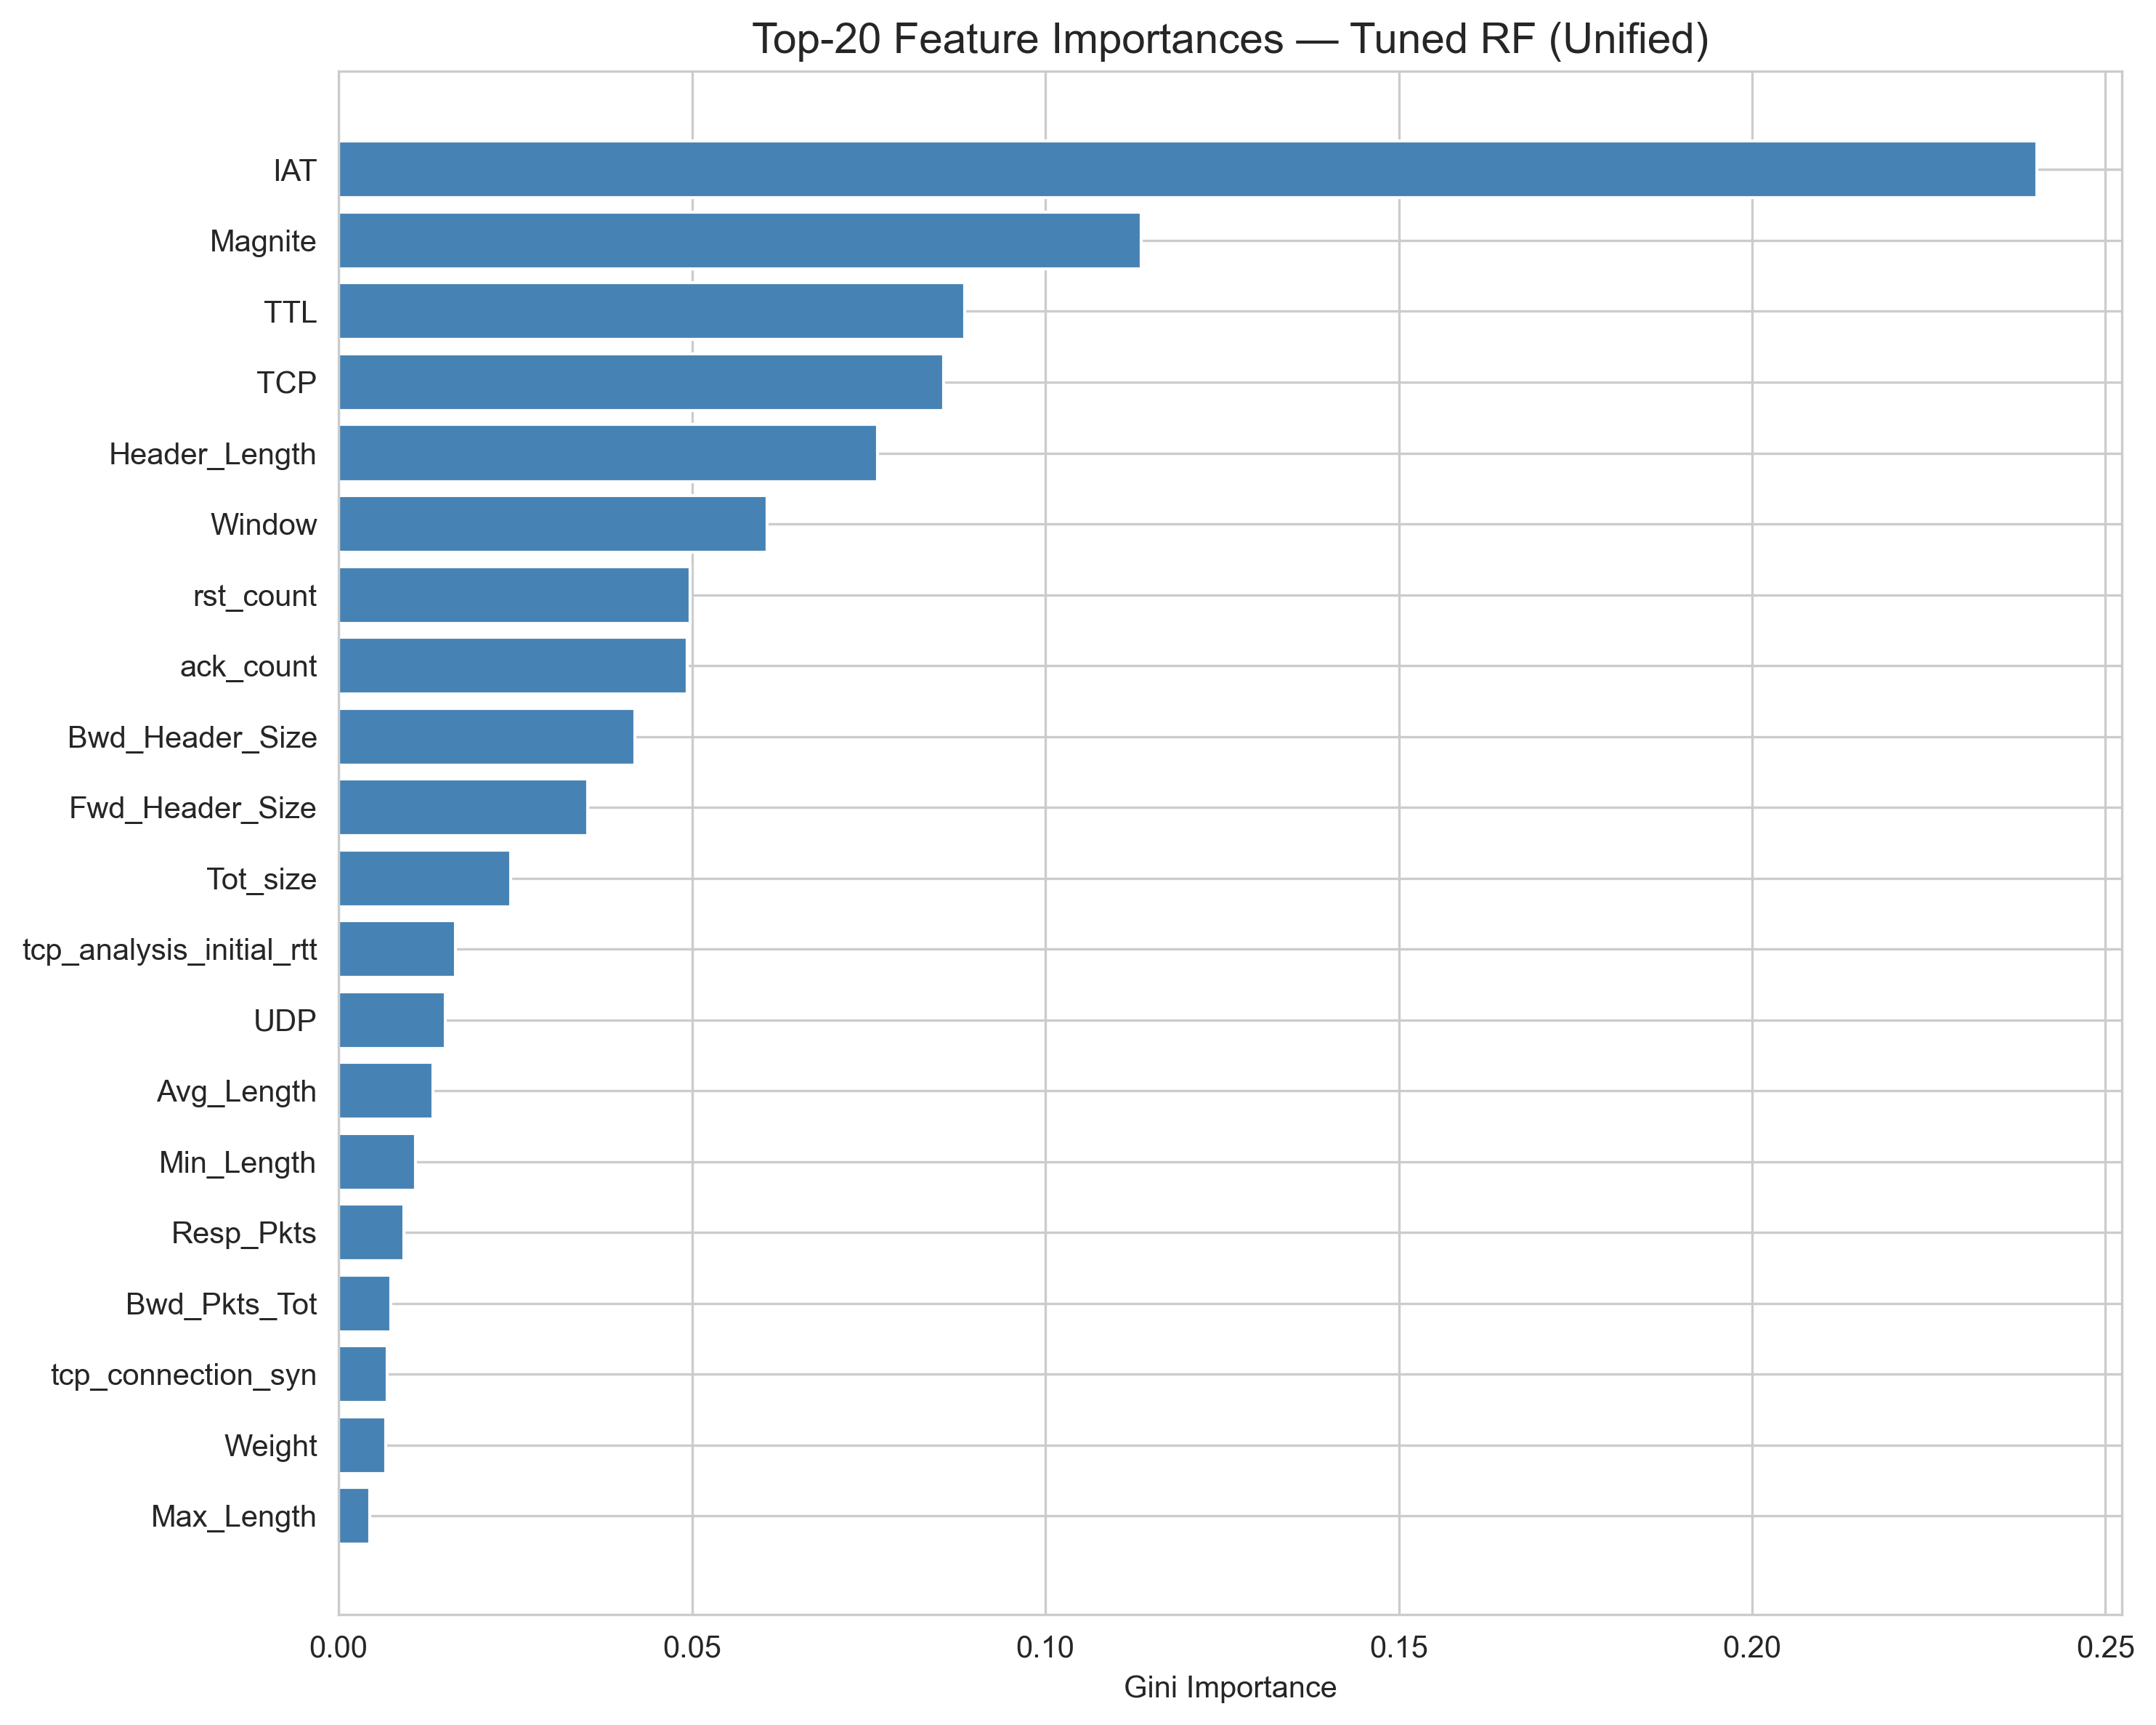
\includegraphics[width=0.85\textwidth]{ch5_rf_feature_importance_unified.png}
\caption{Top-20 feature importances for the tuned Random Forest (Unified regime).}
\label{fig:rf-feature-importance}
\end{figure}

\begin{figure}[H]
\centering
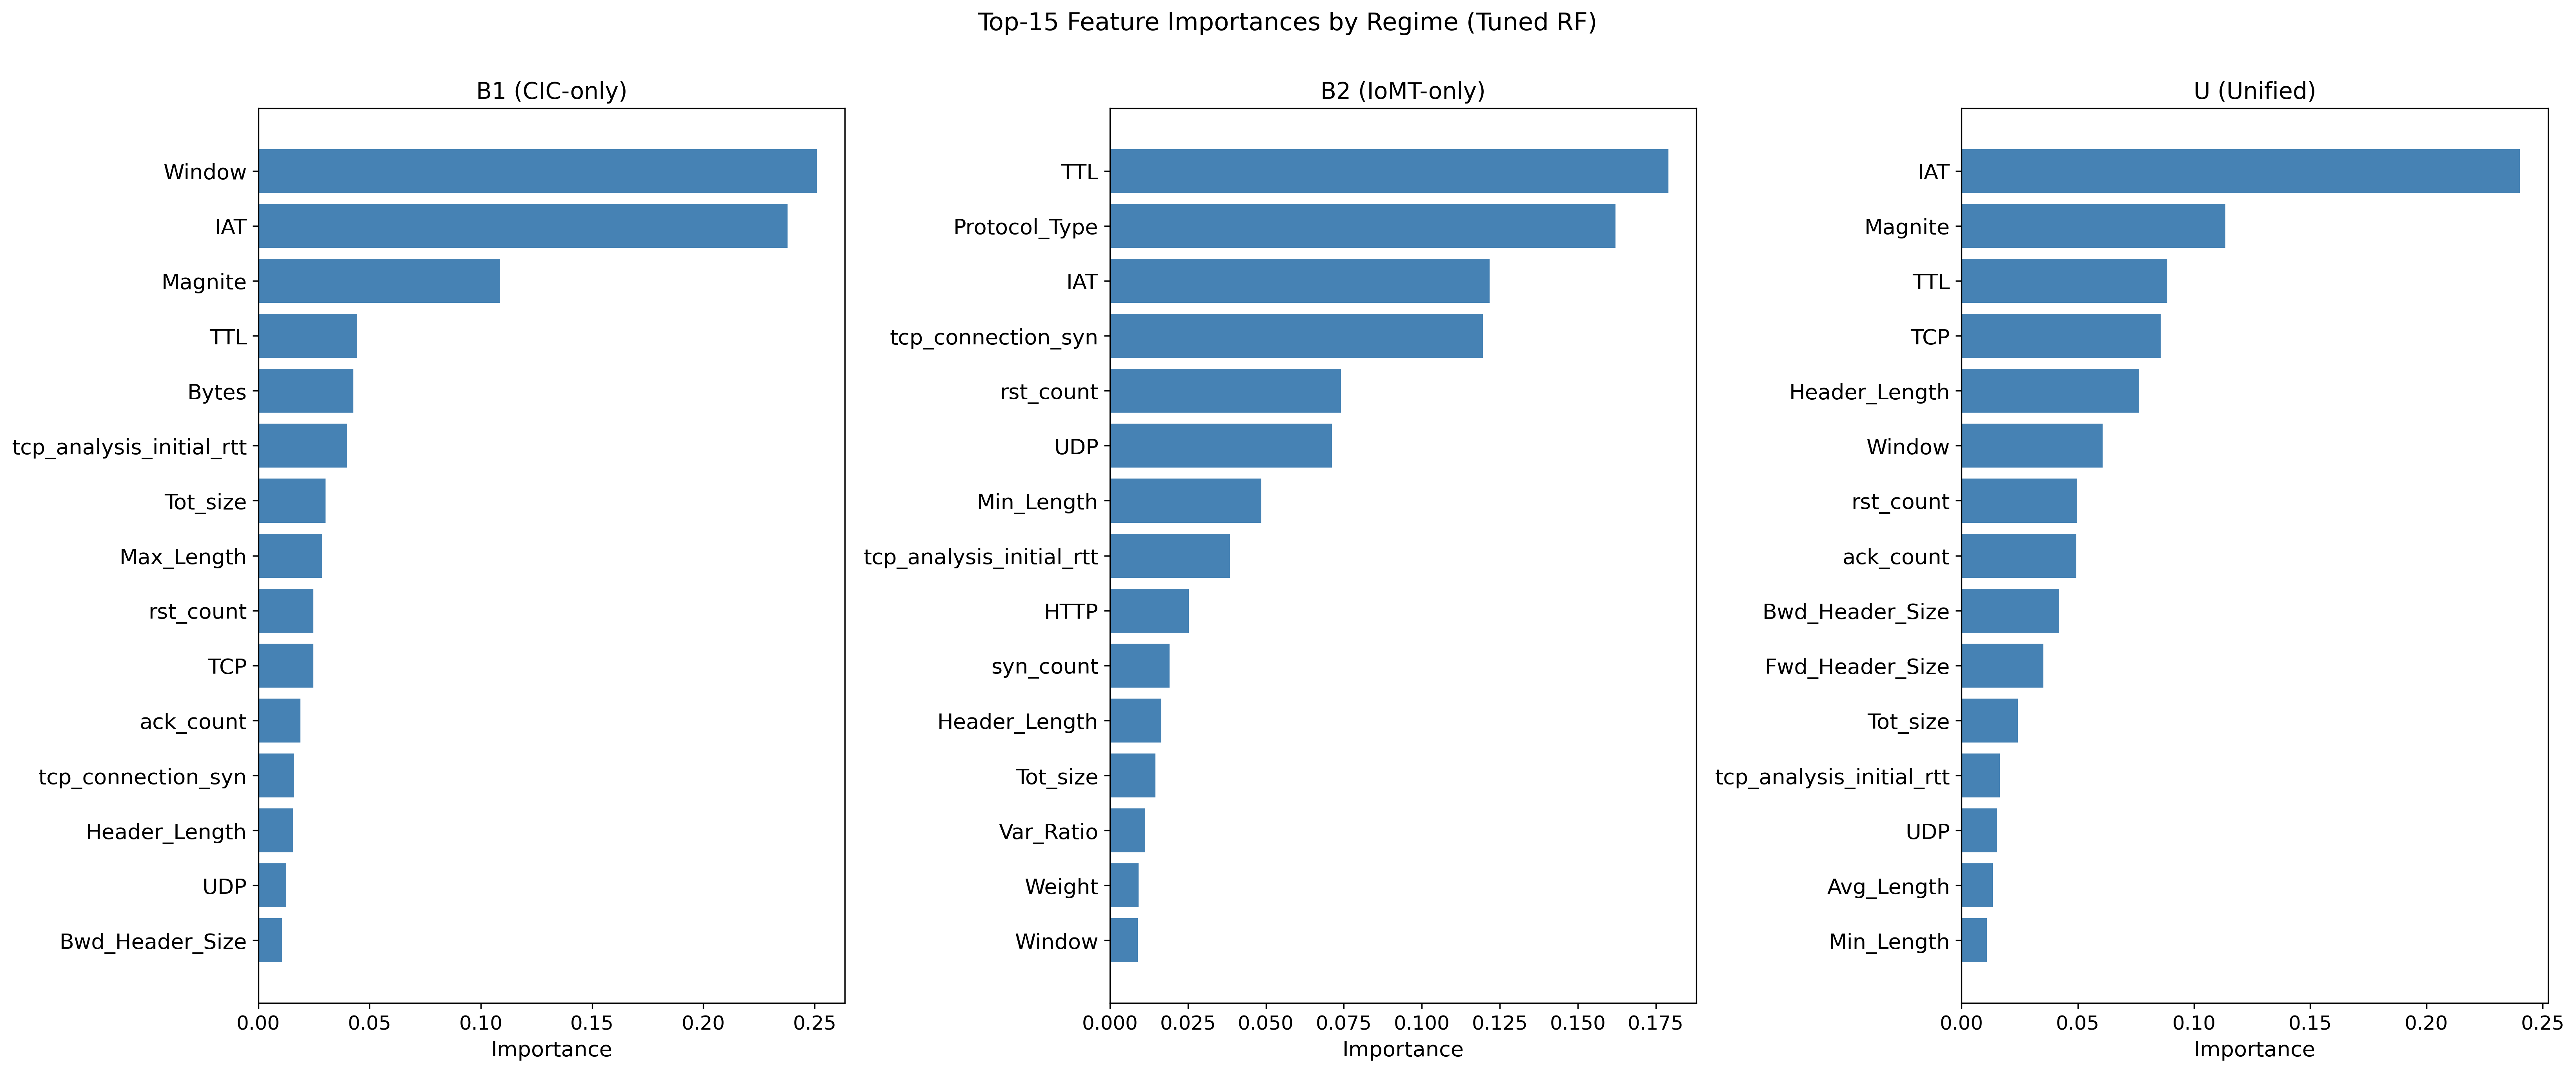
\includegraphics[width=\textwidth]{ch5_rf_feature_importance_comparison.png}
\caption{Feature importance comparison across regimes (tuned RF, top-15).}
\label{fig:rf-fi-comparison}
\end{figure}

\subsubsection{Per-Class Analysis}

Figure~\ref{fig:rf-per-class-f1} compares per-class F1 across tuned regimes on the full test set. Table~\ref{tab:rf-perclass-unified} gives the detailed report for Tuned U.

\begin{figure}[H]
\centering
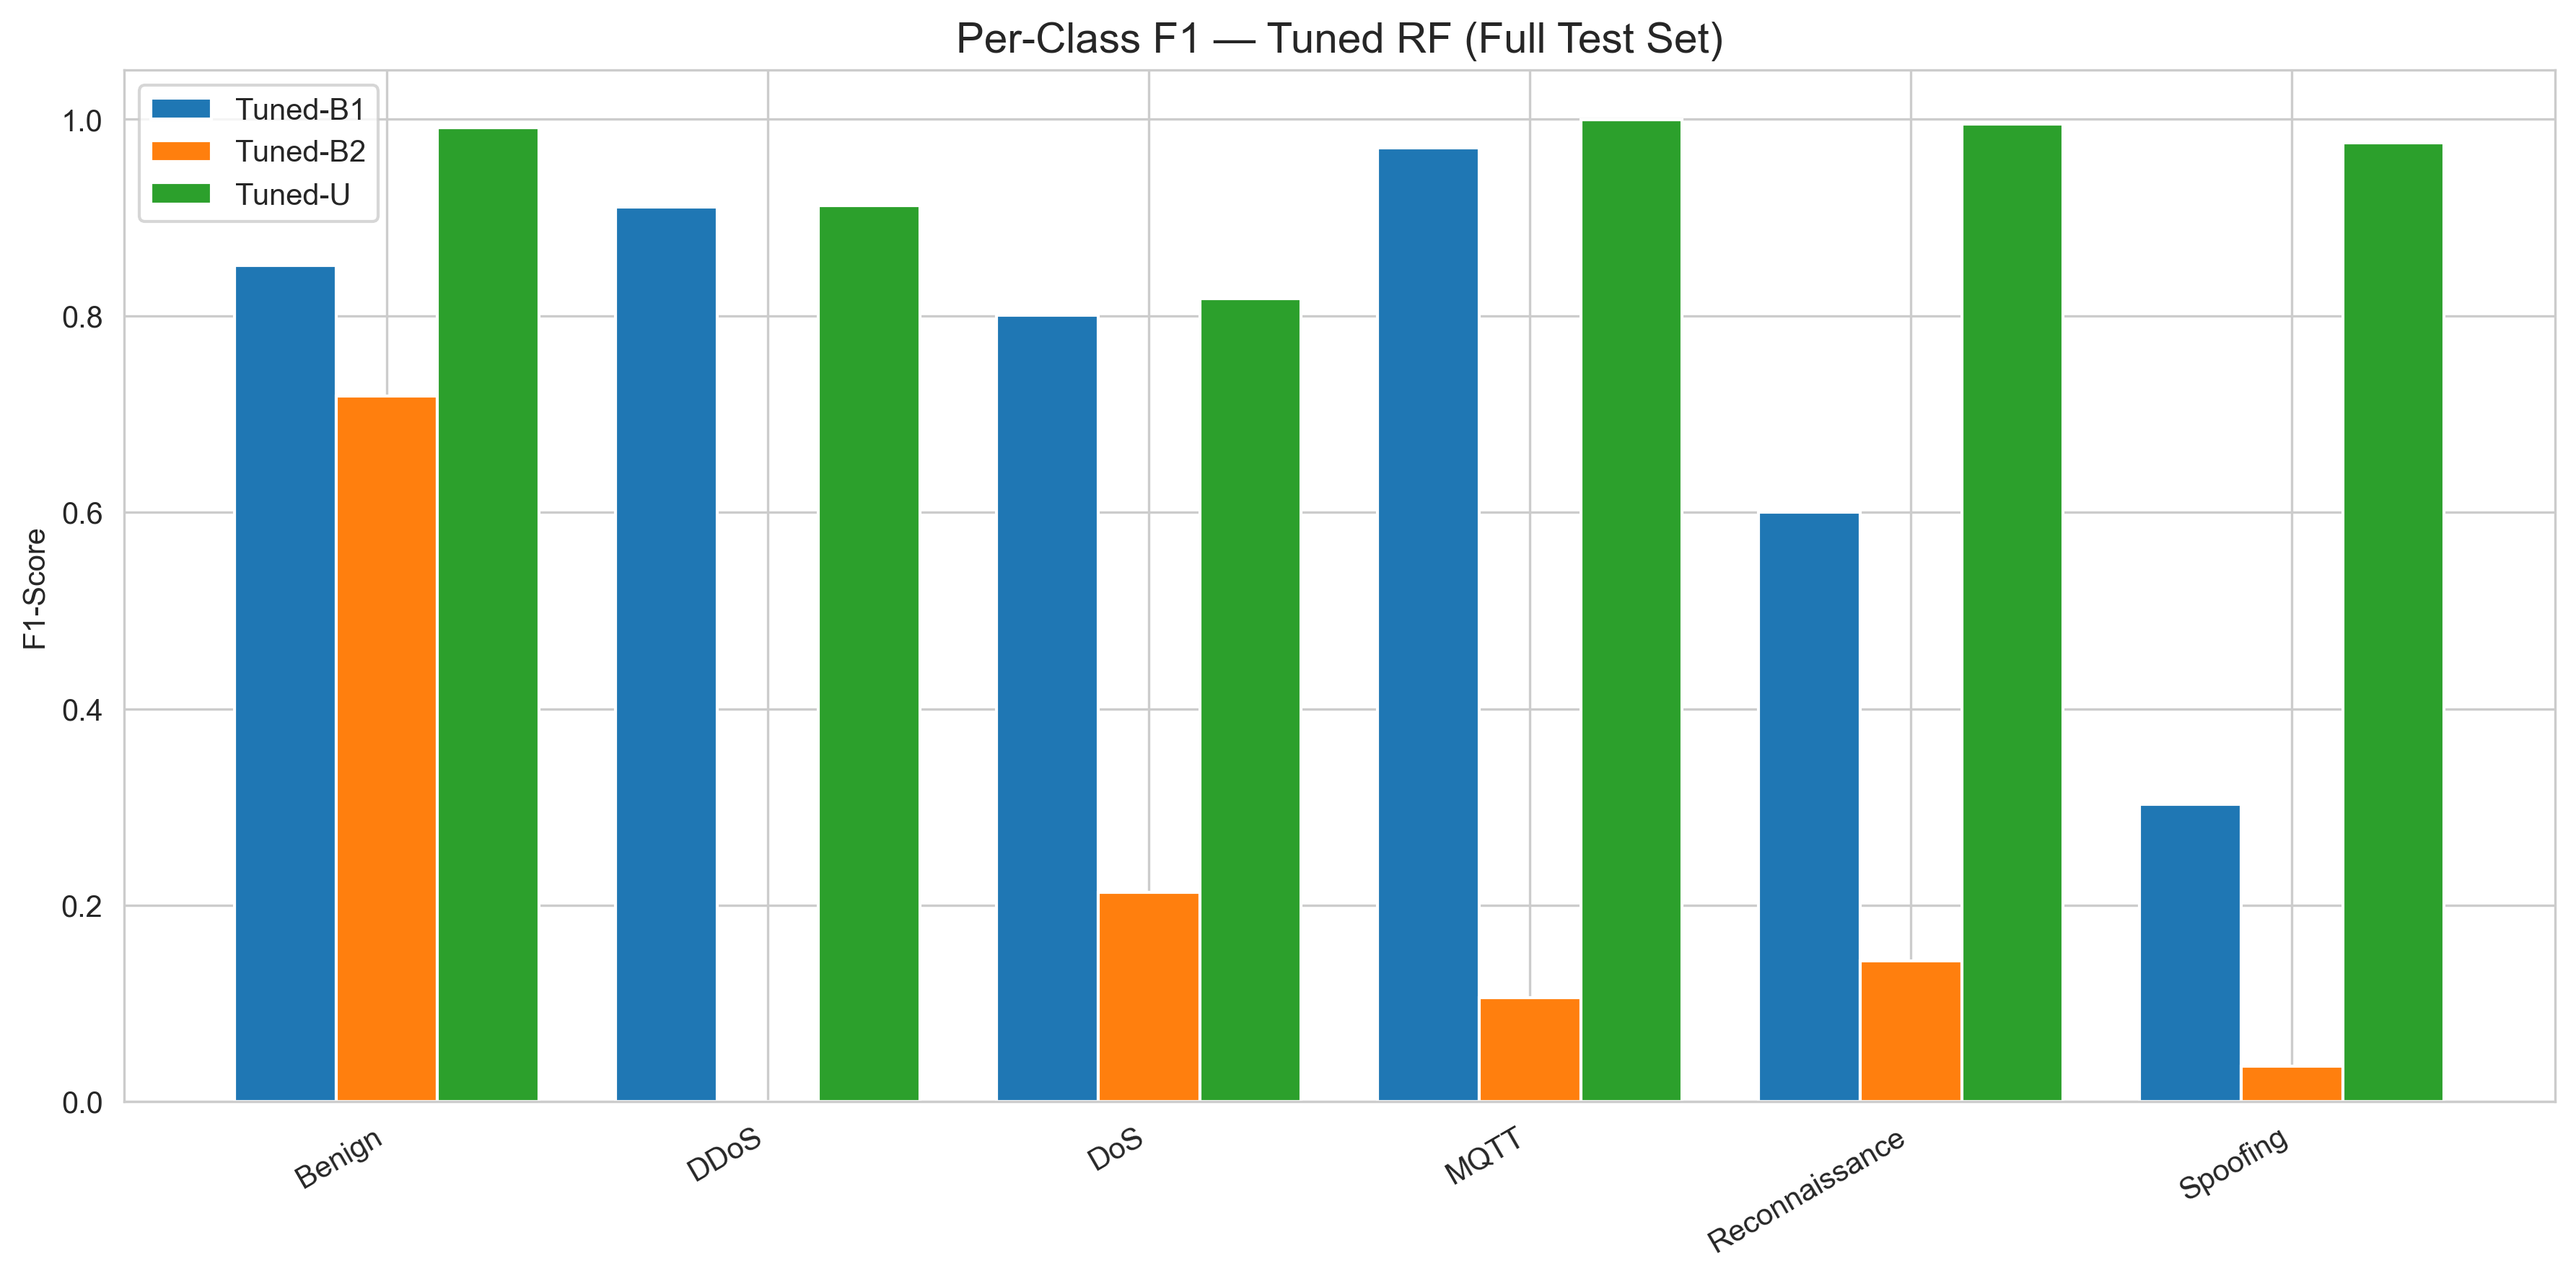
\includegraphics[width=0.85\textwidth]{ch5_rf_per_class_f1.png}
\caption{Per-class F1-score comparison across regimes (tuned RF, full test set).}
\label{fig:rf-per-class-f1}
\end{figure}

\begin{table}[H]
\centering
\caption{Per-class classification report for the tuned unified Random Forest on the full test set (1,201,731 samples).}
\label{tab:rf-perclass-unified}
\small
\begin{tabular}{@{}l r r r r@{}}
\toprule
\textbf{Class} & \textbf{Precision} & \textbf{Recall} & \textbf{F1-Score} & \textbf{Support} \\
\midrule
Benign          & 0.98 & 1.00 & 0.99 &     8,018 \\
DDoS            & 0.97 & 0.86 & 0.91 &   805,244 \\
DoS             & 0.73 & 0.93 & 0.82 &   322,273 \\
MQTT            & 1.00 & 1.00 & 1.00 &    57,891 \\
Reconnaissance  & 1.00 & 0.99 & 1.00 &     6,904 \\
Spoofing        & 0.97 & 0.99 & 0.98 &     1,401 \\
\midrule
Accuracy        &      &      & 0.89 & 1,201,731 \\
Macro avg       & 0.94 & 0.96 & 0.95 & 1,201,731 \\
Weighted avg    & 0.91 & 0.89 & 0.89 & 1,201,731 \\
\bottomrule
\end{tabular}
\end{table}

The Random Forest reproduces the same qualitative structure as the Decision Tree: near-perfect scores on Benign, MQTT, Reconnaissance, and Spoofing, with residual error concentrated in the DDoS/DoS boundary. Macro-F1 on the full test improves slightly relative to the tuned DT (0.9487 vs.\ 0.9480), while weighted-F1 and accuracy are essentially unchanged. Critically, the hypothesis that ensemble voting would substantially reduce the DDoS/DoS confusion is \textbf{not confirmed}: DDoS F1 (0.91) and DoS F1 (0.82) are identical to the tuned DT values, confirming that the source of the confusion is a feature-representation limitation that averaging over decorrelated trees cannot resolve on its own.

\subsubsection{Summary}

\begin{itemize}[nosep]
  \item \textbf{Single-source models remain brittle cross-domain.} Tuned B1 improves IoMT Macro-F1 versus the DT baseline (0.34 vs.\ 0.25) but still fails to generalize. Tuned B2 collapses on the full and CIC slices for the same structural reason as before (no DDoS exposure).
  \item \textbf{Unified RF matches or marginally exceeds unified DT.} Full-test Macro-F1 reaches 0.9487 (+0.7 percentage points over tuned DT). Cross-domain slices for Tuned U remain strong (CIC 0.9285, IoMT 0.8329 before the absent-class caveat above).
  \item \textbf{Ensemble variance reduction.} The selected shallow trees with \texttt{max\_samples}=0.8 and moderate \texttt{n\_estimators} (200--300) provide a stable bias--variance trade-off without the extreme memory cost of very large unrestricted forests.
  \item \textbf{DDoS/DoS boundary: hypothesis not confirmed.} Despite the theoretical expectation that ensemble voting would smooth the DDoS$\leftrightarrow$DoS decision boundary, per-class F1 scores for both classes are indistinguishable from the Decision Tree (DDoS: 0.91, DoS: 0.82 in both cases). This null result reinforces that the boundary confusion is driven by absent multi-source diversity features in the current 58-feature window representation, not by model capacity.
\end{itemize}

\subsection{XGBoost Classifier}
\label{subsec:xgboost}

Gradient boosted trees (XGBoost) provide a third point on the bias--variance spectrum. Training uses histogram-based tree construction (\texttt{tree\_method='hist'}) and per-sample weights for class imbalance. Because the IoMT-only regime (B2) lacks the global DDoS class in its training partition, the implementation remaps the present global label indices to contiguous integers during XGBoost's \texttt{multi:softmax} fit and maps predictions back to the global six-class space for evaluation---mirroring how the encoder still defines a common confusion-matrix layout.

\subsubsection{Baseline Results}

Table~\ref{tab:xgb-baseline} reports baseline XGBoost performance ($n_{\text{estimators}}=100$, default learning rate).

\begin{table}[H]
\centering
\caption{Baseline XGBoost evaluation matrix.}
\label{tab:xgb-baseline}
\small
\begin{tabular}{@{}l l c c c@{}}
\toprule
\textbf{Regime} & \textbf{Test slice} & \textbf{Macro-F1} & \textbf{Weighted-F1} & \textbf{Accuracy} \\
\midrule
B1 (CIC-only) & CIC (in-domain)  & 0.9376 & 0.8923 & 0.8888 \\
B1 (CIC-only) & IoMT (cross)     & 0.3576 & 0.5052 & 0.5238 \\
B1 (CIC-only) & Full             & 0.7629 & 0.8834 & 0.8804 \\
\midrule
B2 (IoMT-only) & IoMT (in-domain) & 0.8333 & 0.9999 & 0.9999 \\
B2 (IoMT-only) & CIC (cross)      & 0.0900 & 0.0862 & 0.1061 \\
B2 (IoMT-only) & Full             & 0.3602 & 0.0990 & 0.1266 \\
\midrule
U (Unified)    & CIC              & 0.9380 & 0.8924 & 0.8889 \\
U (Unified)    & IoMT             & 0.8333 & 1.0000 & 1.0000 \\
U (Unified)    & Full             & \textbf{0.9520} & 0.8947 & 0.8914 \\
\bottomrule
\end{tabular}
\end{table}

\subsubsection{Tuned Results}

Table~\ref{tab:xgb-tuned} reports tuned XGBoost results. Table~\ref{tab:xgb-best-params} lists the best hyperparameters (CV macro-F1 on the search subsample / full B2 training set).

\begin{table}[H]
\centering
\caption{Tuned XGBoost evaluation matrix.}
\label{tab:xgb-tuned}
\small
\begin{tabular}{@{}l l c c c@{}}
\toprule
\textbf{Regime} & \textbf{Test slice} & \textbf{Macro-F1} & \textbf{Weighted-F1} & \textbf{Accuracy} \\
\midrule
Tuned B1 & CIC (in-domain)  & 0.9410 & 0.8951 & 0.8918 \\
Tuned B1 & IoMT (cross)     & 0.2724 & 0.4057 & 0.4394 \\
Tuned B1 & Full             & 0.7199 & 0.8838 & 0.8814 \\
\midrule
Tuned B2 & IoMT (in-domain) & 0.8333 & 1.0000 & 1.0000 \\
Tuned B2 & CIC (cross)      & 0.1079 & 0.1045 & 0.1810 \\
Tuned B2 & Full             & 0.3708 & 0.1161 & 0.1998 \\
\midrule
Tuned U  & CIC              & 0.9382 & 0.8931 & 0.8897 \\
Tuned U  & IoMT             & 0.8333 & 0.9999 & 0.9999 \\
Tuned U  & Full             & \textbf{0.9522} & 0.8954 & 0.8922 \\
\bottomrule
\end{tabular}
\end{table}

\paragraph{Note on Macro-F1 (IoMT slice, Tuned U).}
The same absent-class effect as in Tables~\ref{tab:dt-tuned} and~\ref{tab:rf-tuned} applies: IoMT test traffic carries no DDoS label, so the global Macro-F1 on that slice (0.8333) averages over a zero-score DDoS column.

\begin{table}[H]
\centering
\caption{Best hyperparameters per regime (XGBoost, 50-iteration RandomizedSearchCV). Abbreviations: mcw $=$ \texttt{min\_child\_weight}, cbt $=$ \texttt{colsample\_bytree}, $\lambda$ $=$ \texttt{reg\_lambda}, $\alpha$ $=$ \texttt{reg\_alpha}.}
\label{tab:xgb-best-params}
\scriptsize
\begin{tabular}{@{}l c c c c c c c c c c@{}}
\toprule
\textbf{Reg.} & \textbf{lr} & \textbf{trees} & \textbf{depth} & \textbf{mcw} & \textbf{subs.} & \textbf{cbt} & $\gamma$ & $\lambda$ & $\alpha$ & \textbf{CV F1m} \\
\midrule
B1 & 0.10 & 500 & 12 & 20 & 0.6 & 0.9 & 0.1 & 1 & 0.1 & 0.9437 \\
B2 & 0.20 & 200 & 12 & 1  & 0.9 & 0.8 & 0 & 0.01 & 1 & 0.9999 \\
U  & 0.03 & 500 & 9  & 5  & 0.6 & 0.9 & 0 & 0.01 & 0 & 0.9575 \\
\bottomrule
\end{tabular}
\end{table}

\subsubsection{Cross-Domain Analysis}

Figure~\ref{fig:xgb-confusion-unified} shows the normalized confusion matrix for the tuned unified XGBoost on the full test set. Figure~\ref{fig:xgb-cm-xd} shows the cross-domain matrices for B1$\to$IoMT and B2$\to$CIC.

\begin{figure}[H]
\centering
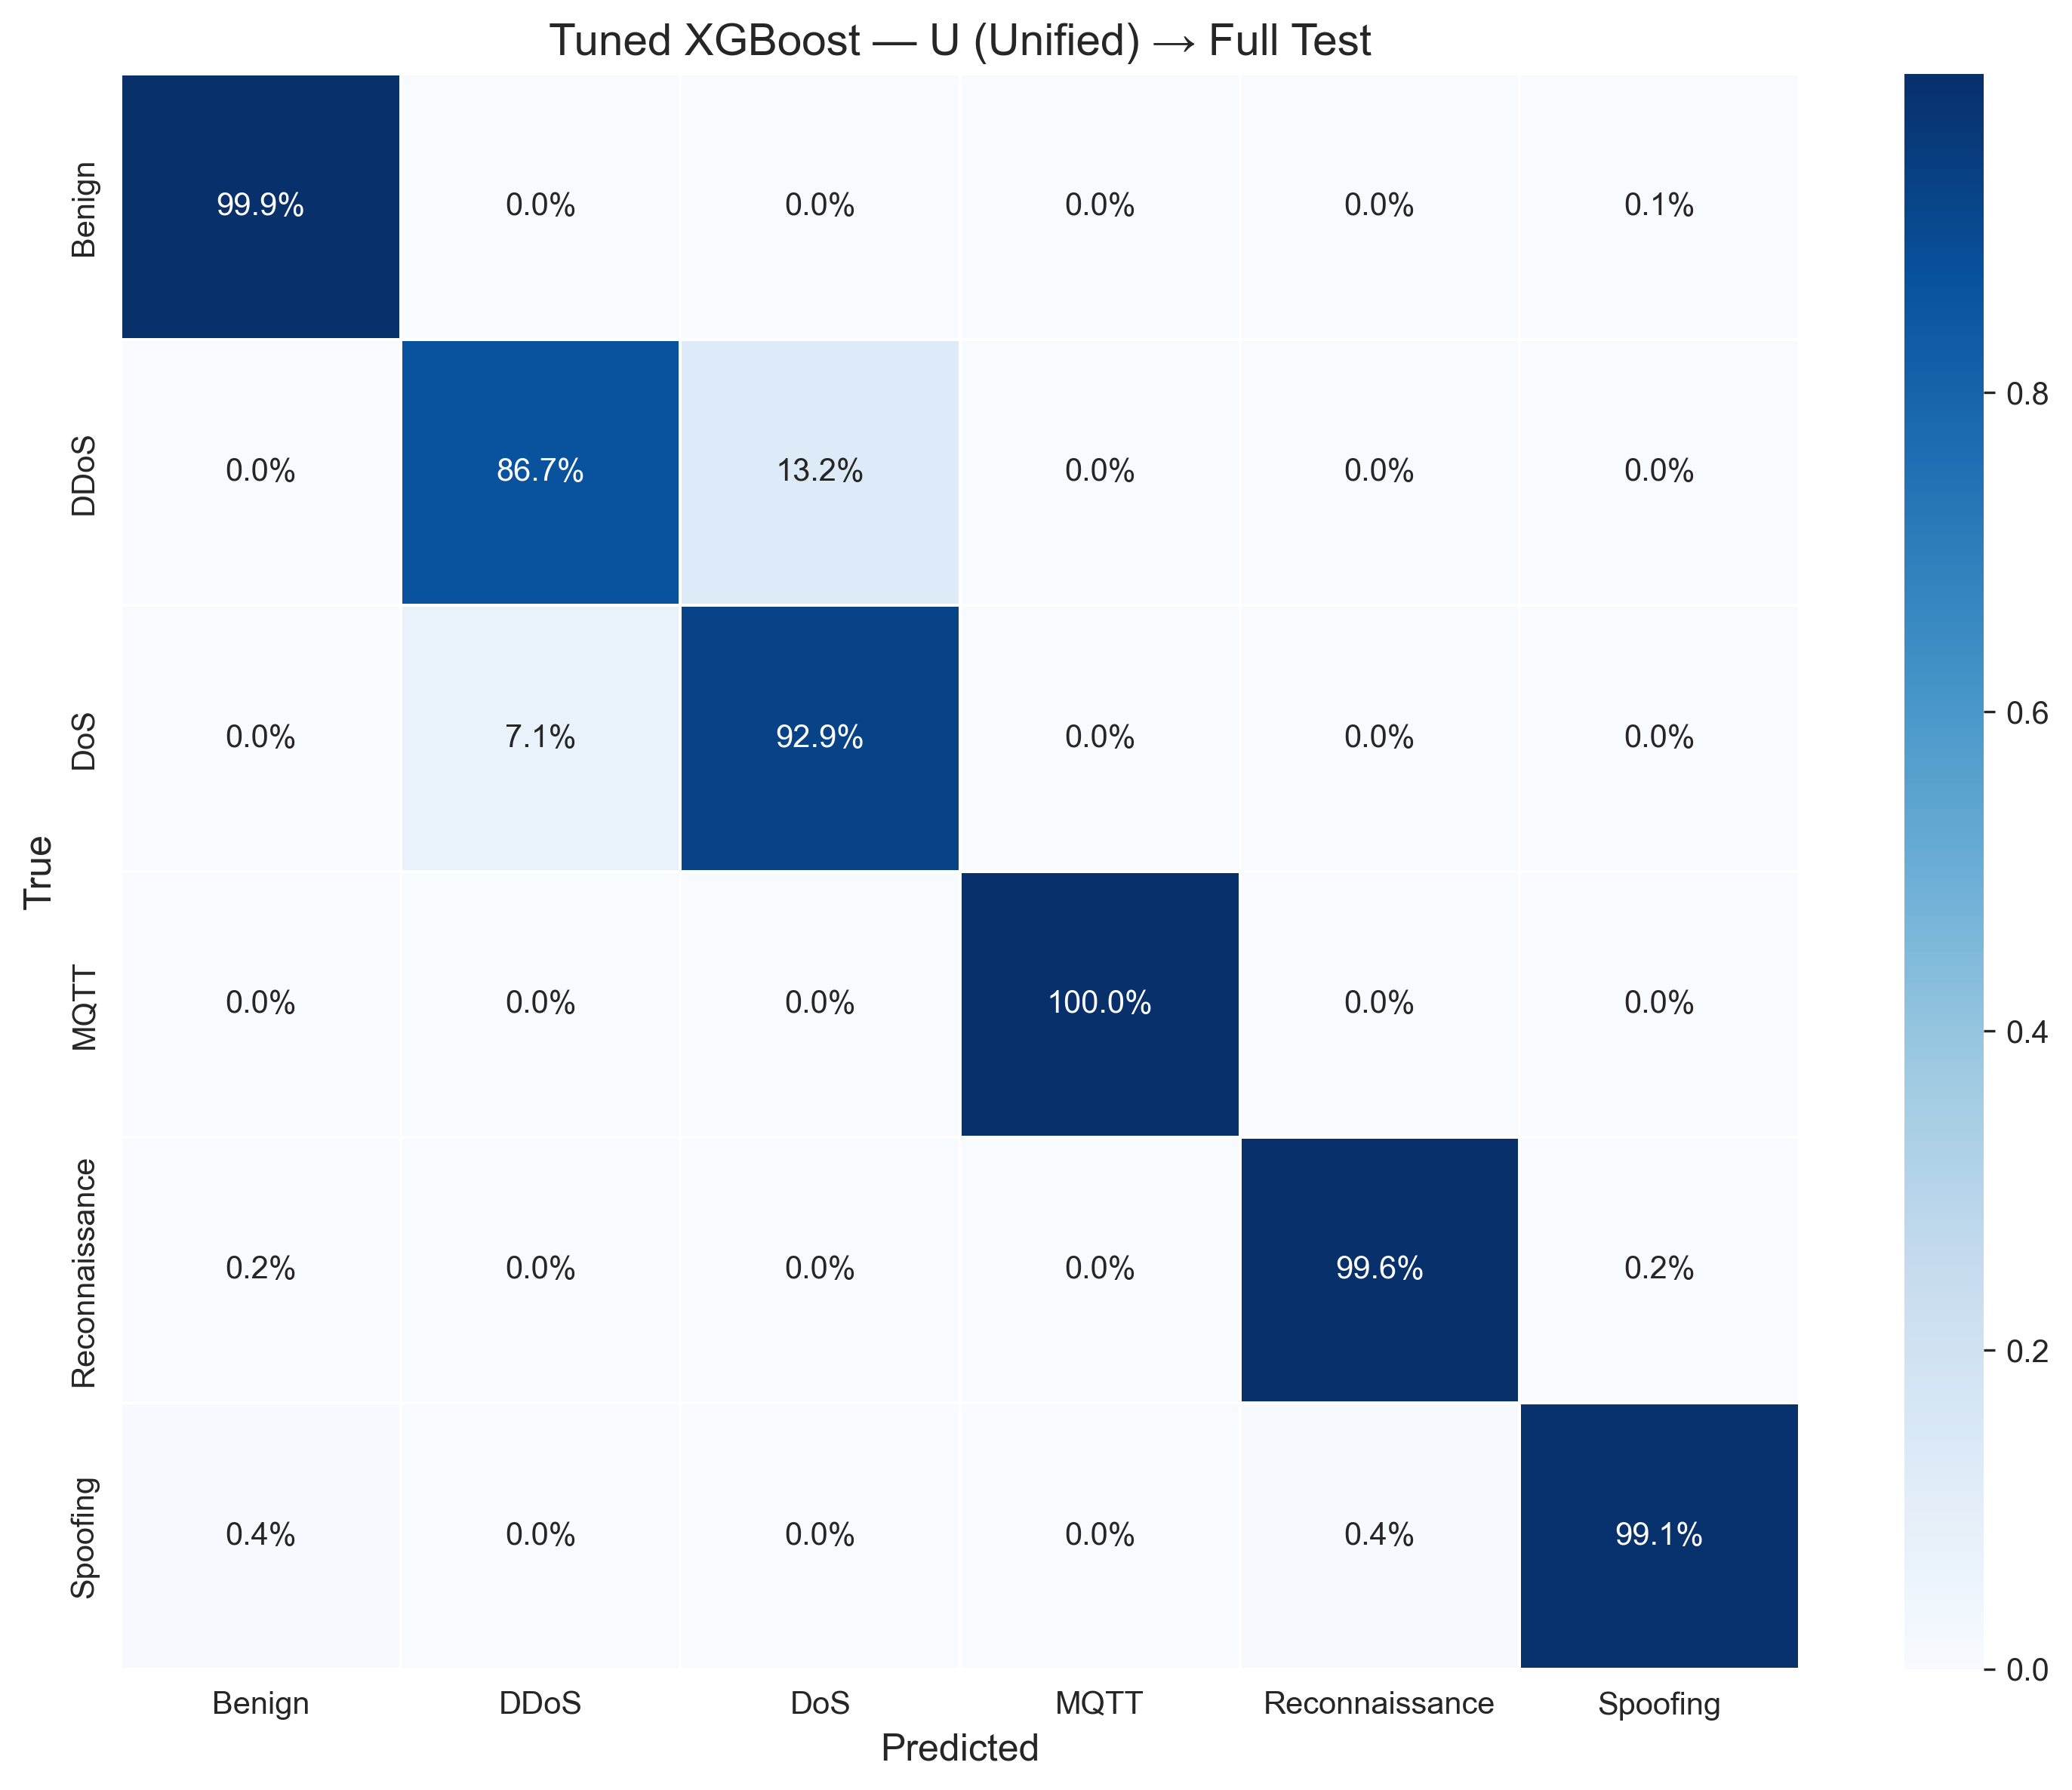
\includegraphics[width=0.75\textwidth]{ch5_xgb_cm_u_full.png}
\caption{Normalized confusion matrix --- Tuned XGBoost (Unified) on the full test set.}
\label{fig:xgb-confusion-unified}
\end{figure}

\begin{figure}[H]
\centering
\begin{subfigure}[b]{0.48\textwidth}
  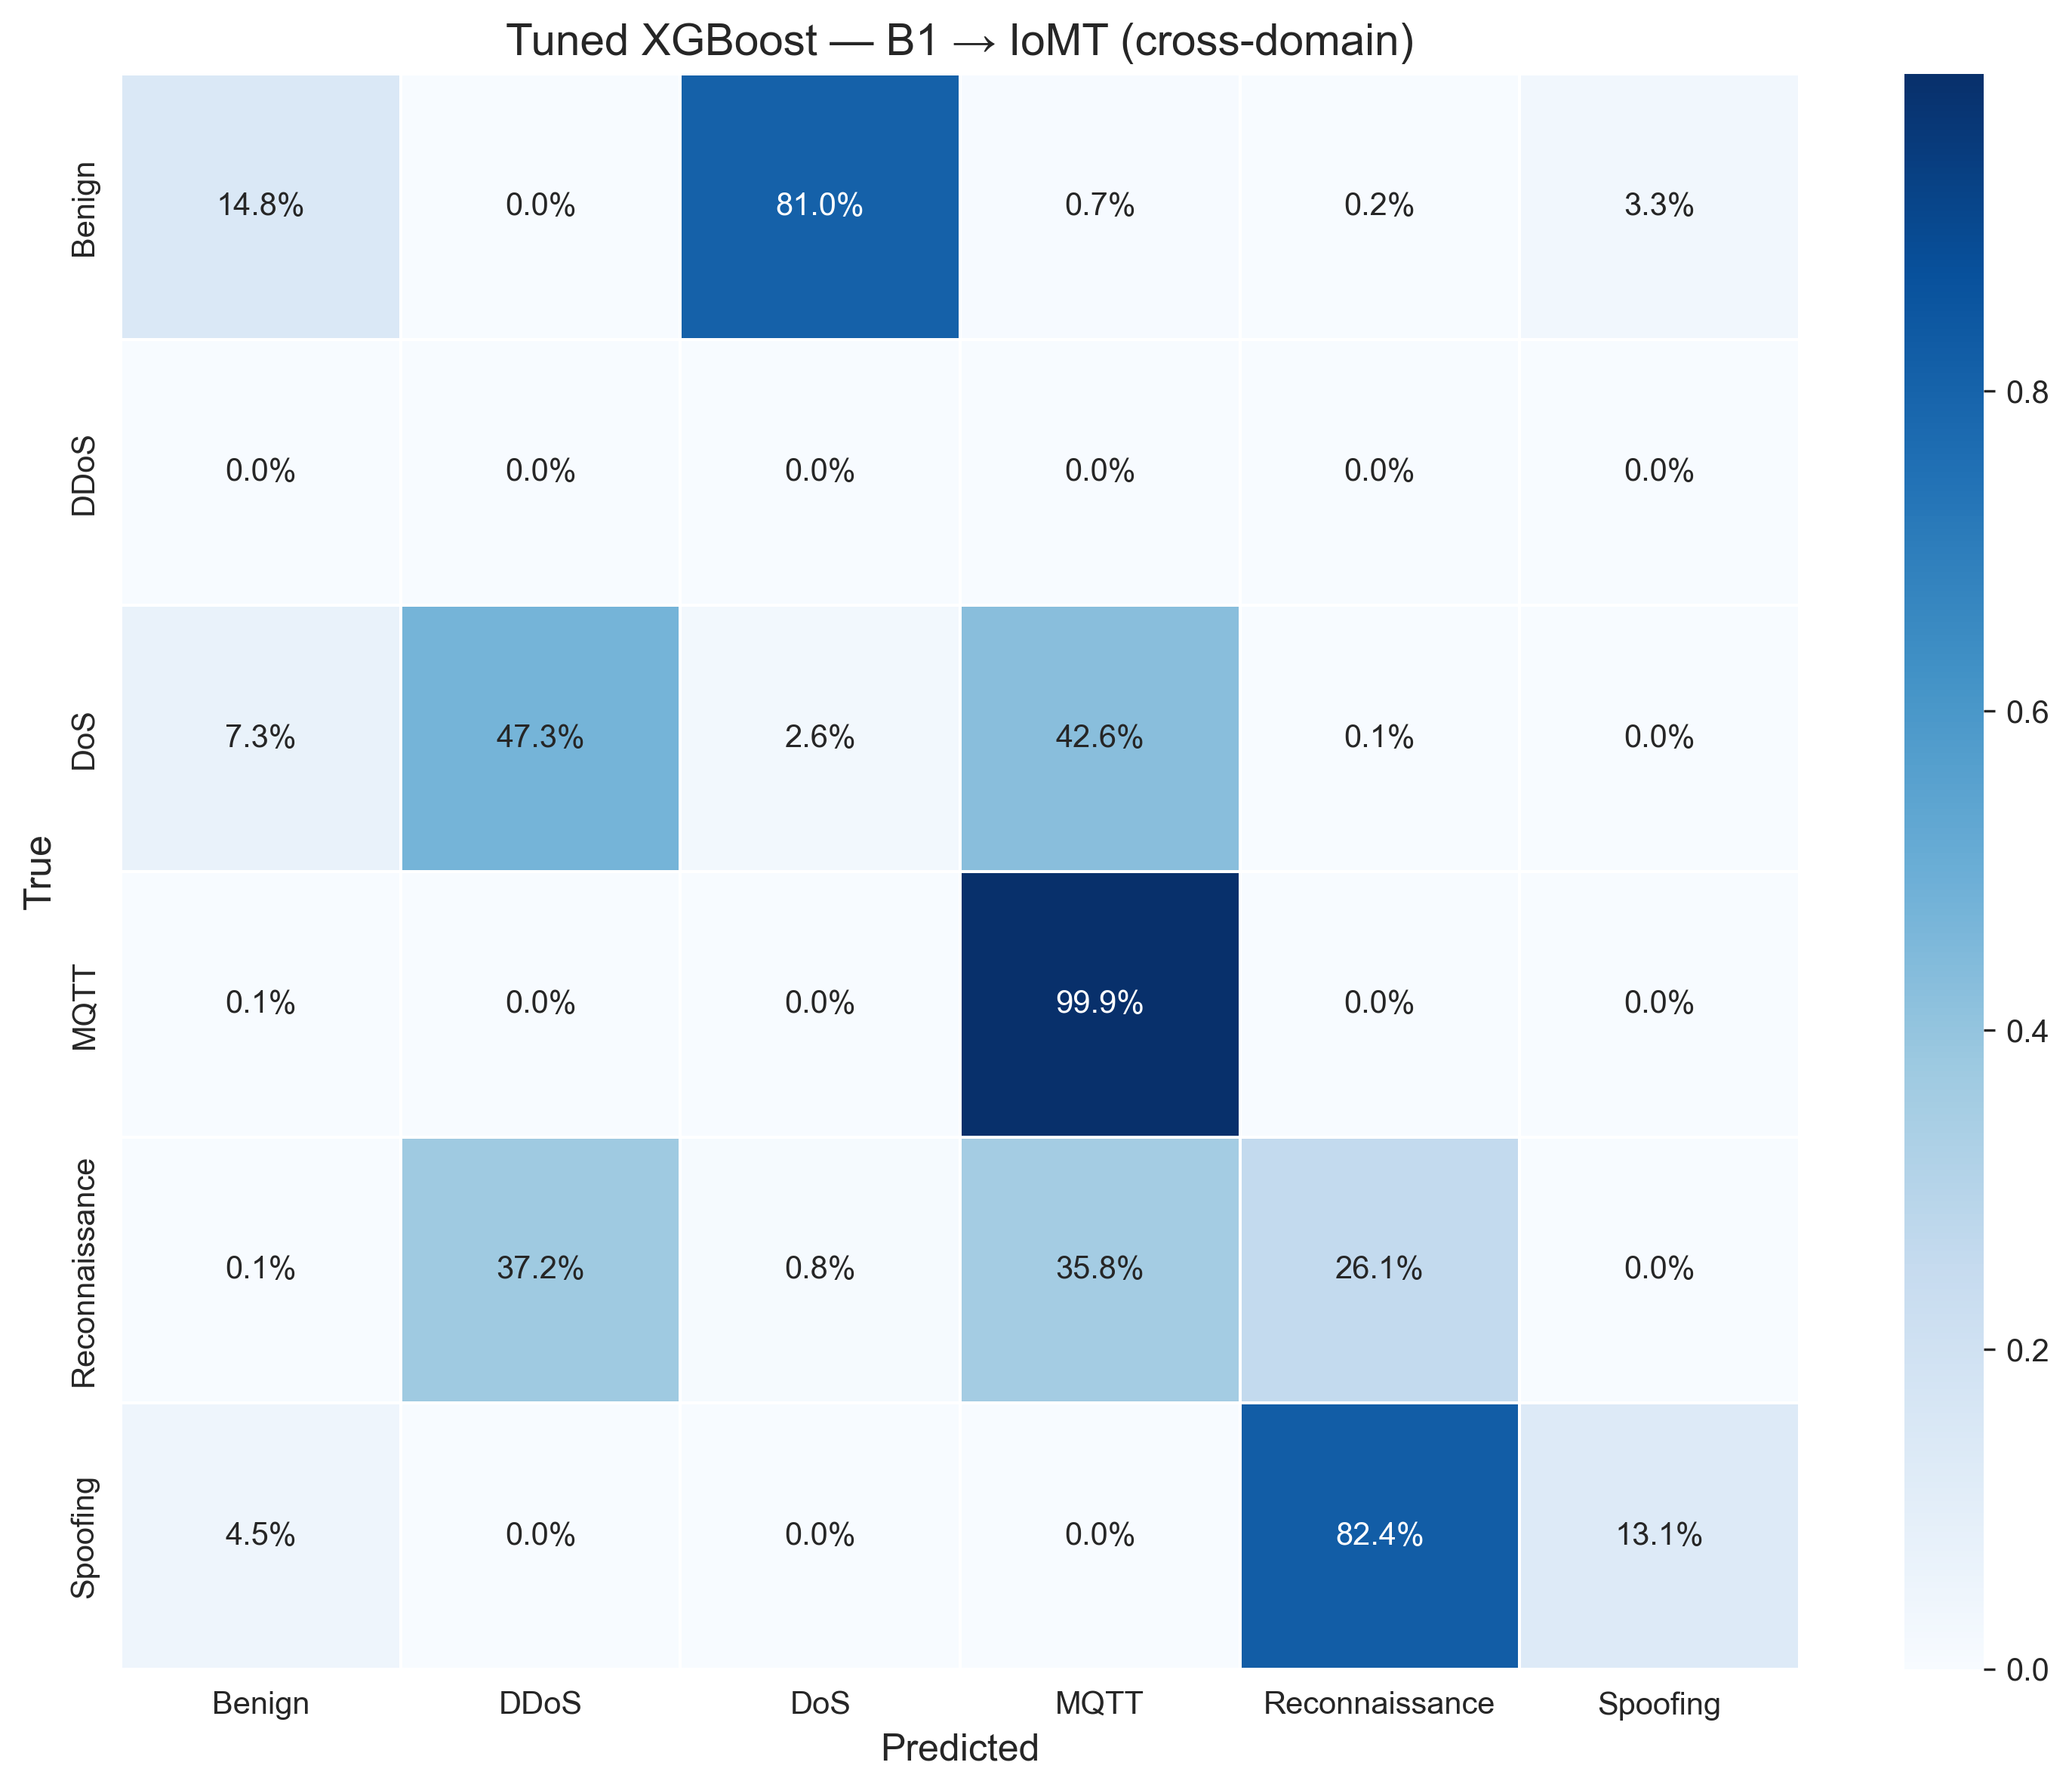
\includegraphics[width=\textwidth]{ch5_xgb_cm_b1_xd_iomt.png}
  \caption{B1 (CIC-only) $\to$ IoMT test}
\end{subfigure}
\hfill
\begin{subfigure}[b]{0.48\textwidth}
  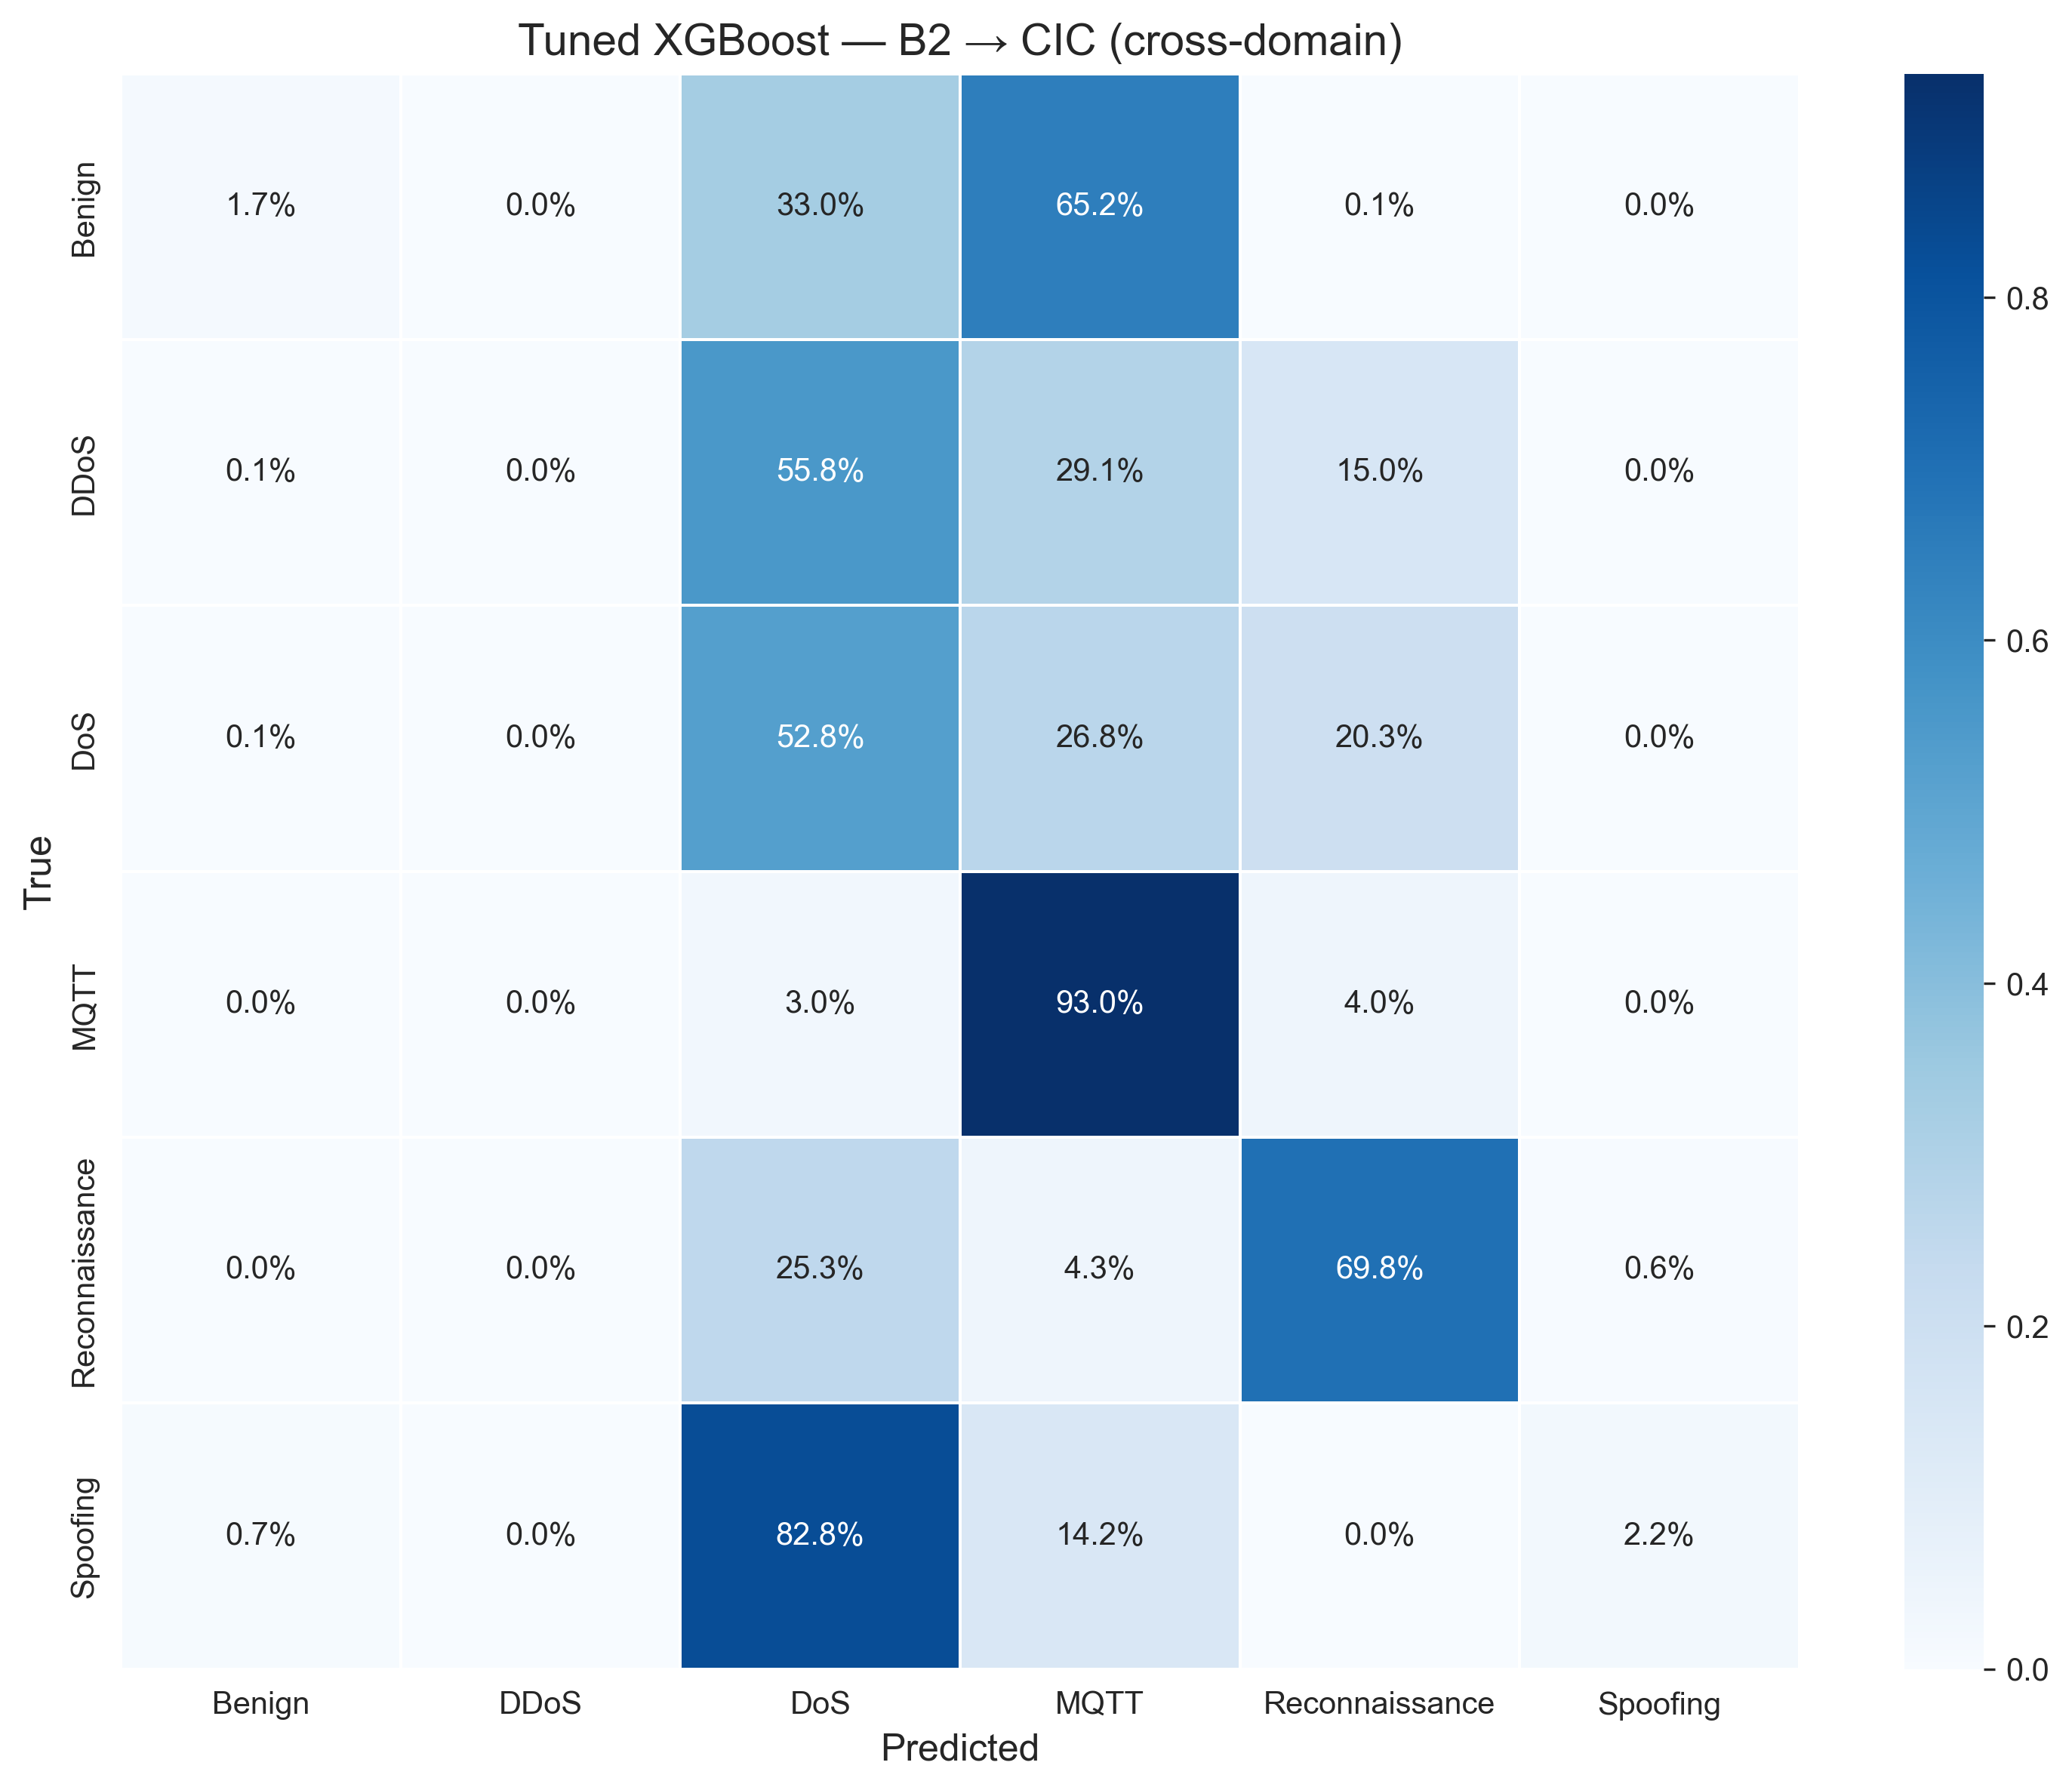
\includegraphics[width=\textwidth]{ch5_xgb_cm_b2_xd_cic.png}
  \caption{B2 (IoMT-only) $\to$ CIC test}
\end{subfigure}
\caption{Cross-domain confusion matrices for tuned XGBoost models.}
\label{fig:xgb-cm-xd}
\end{figure}

The unified XGBoost confusion matrix (Figure~\ref{fig:xgb-confusion-unified}) reproduces the same dominant DDoS$\leftrightarrow$DoS error pattern observed for DT and RF, with all other class pairs near-zero error. The B1$\to$IoMT cross-domain score (Macro-F1 = 0.2724) is lower than the Random Forest equivalent (0.3423), likely because the XGBoost hyperparameters were tuned on a 300k-row subsample of the CIC training data, which may have introduced a tighter fit to the CIC distribution and reduced out-of-distribution generalization. The B2$\to$CIC slice (0.1079) remains poor for the structural reason shared by all three classifiers: DDoS traffic is entirely absent from the B2 training partition, making it impossible for any model in that regime to produce correct predictions on the DDoS-dominated CIC test slice.

\subsubsection{Feature Importance}

Figure~\ref{fig:xgb-feature-importance} shows the top-20 gain-based feature importances for the tuned unified XGBoost model, and Figure~\ref{fig:xgb-fi-comparison} compares importance rankings across all three regimes (top-15). XGBoost's gain importance reflects the average improvement in the loss function per split on a given feature, providing a complementary perspective to the Gini importance used by Decision Tree and Random Forest.

\begin{figure}[H]
\centering
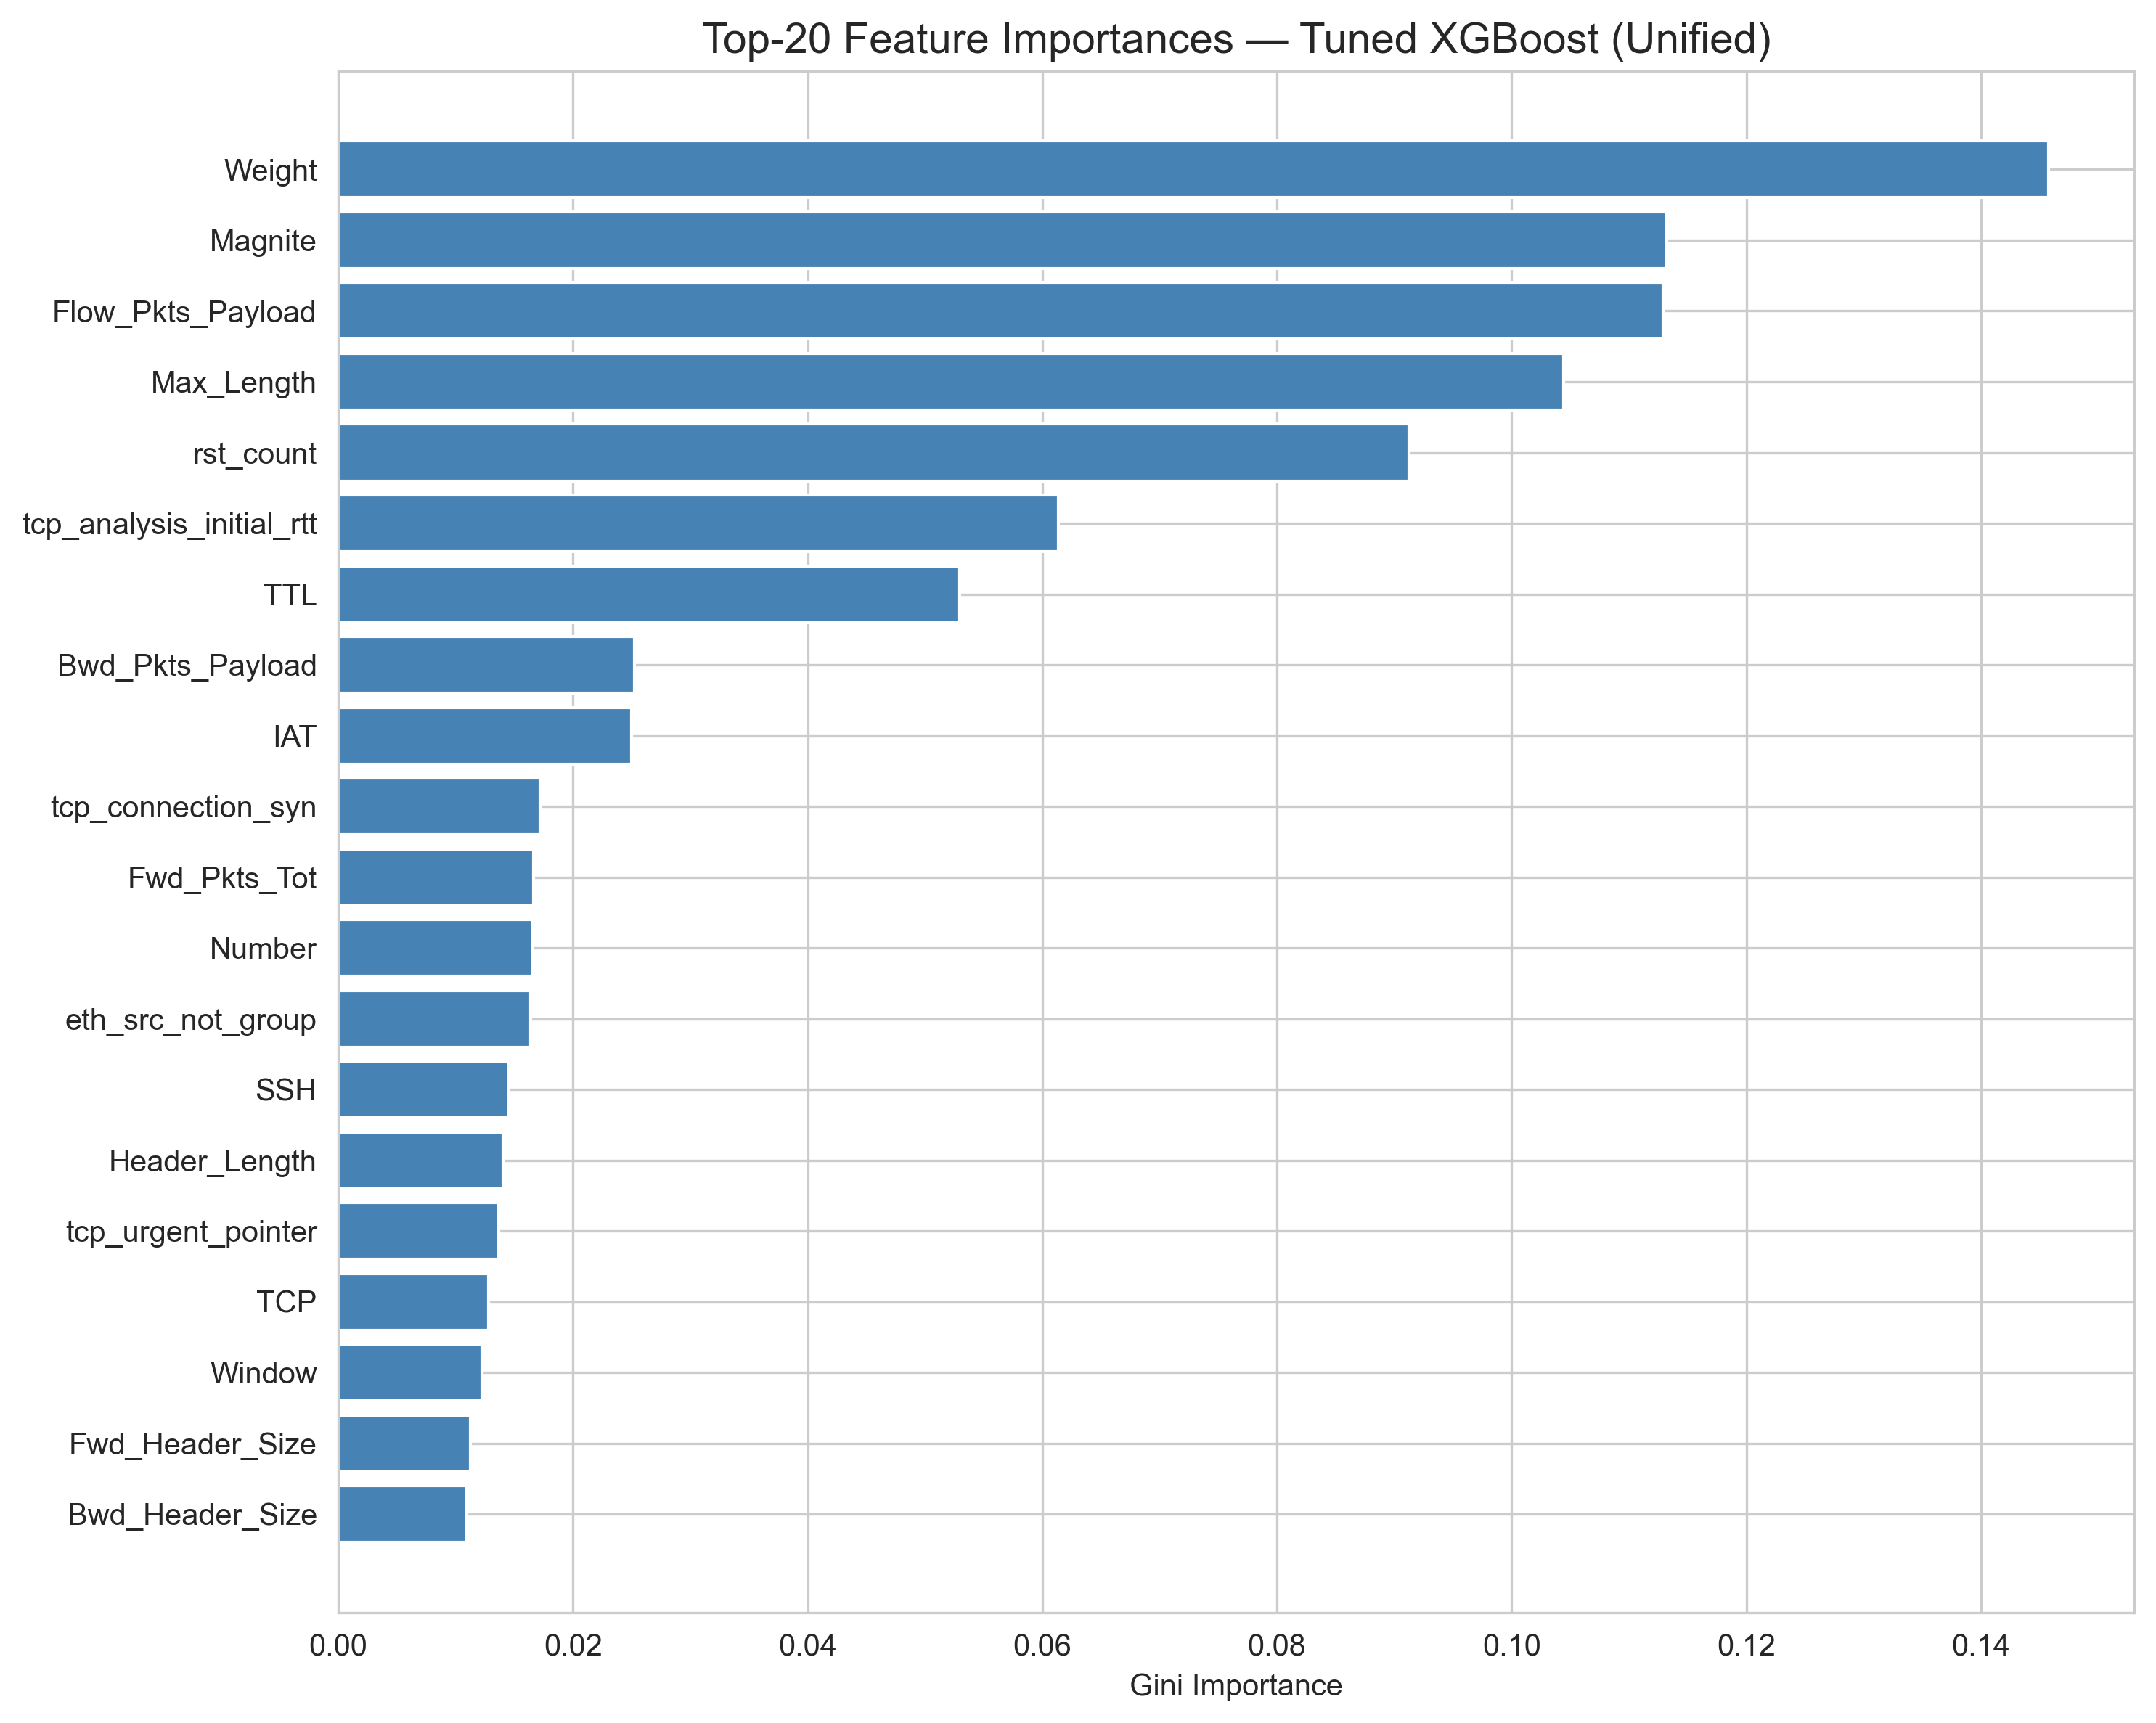
\includegraphics[width=0.85\textwidth]{ch5_xgb_feature_importance_unified.png}
\caption{Top-20 feature importances for the tuned XGBoost (Unified regime).}
\label{fig:xgb-feature-importance}
\end{figure}

\begin{figure}[H]
\centering
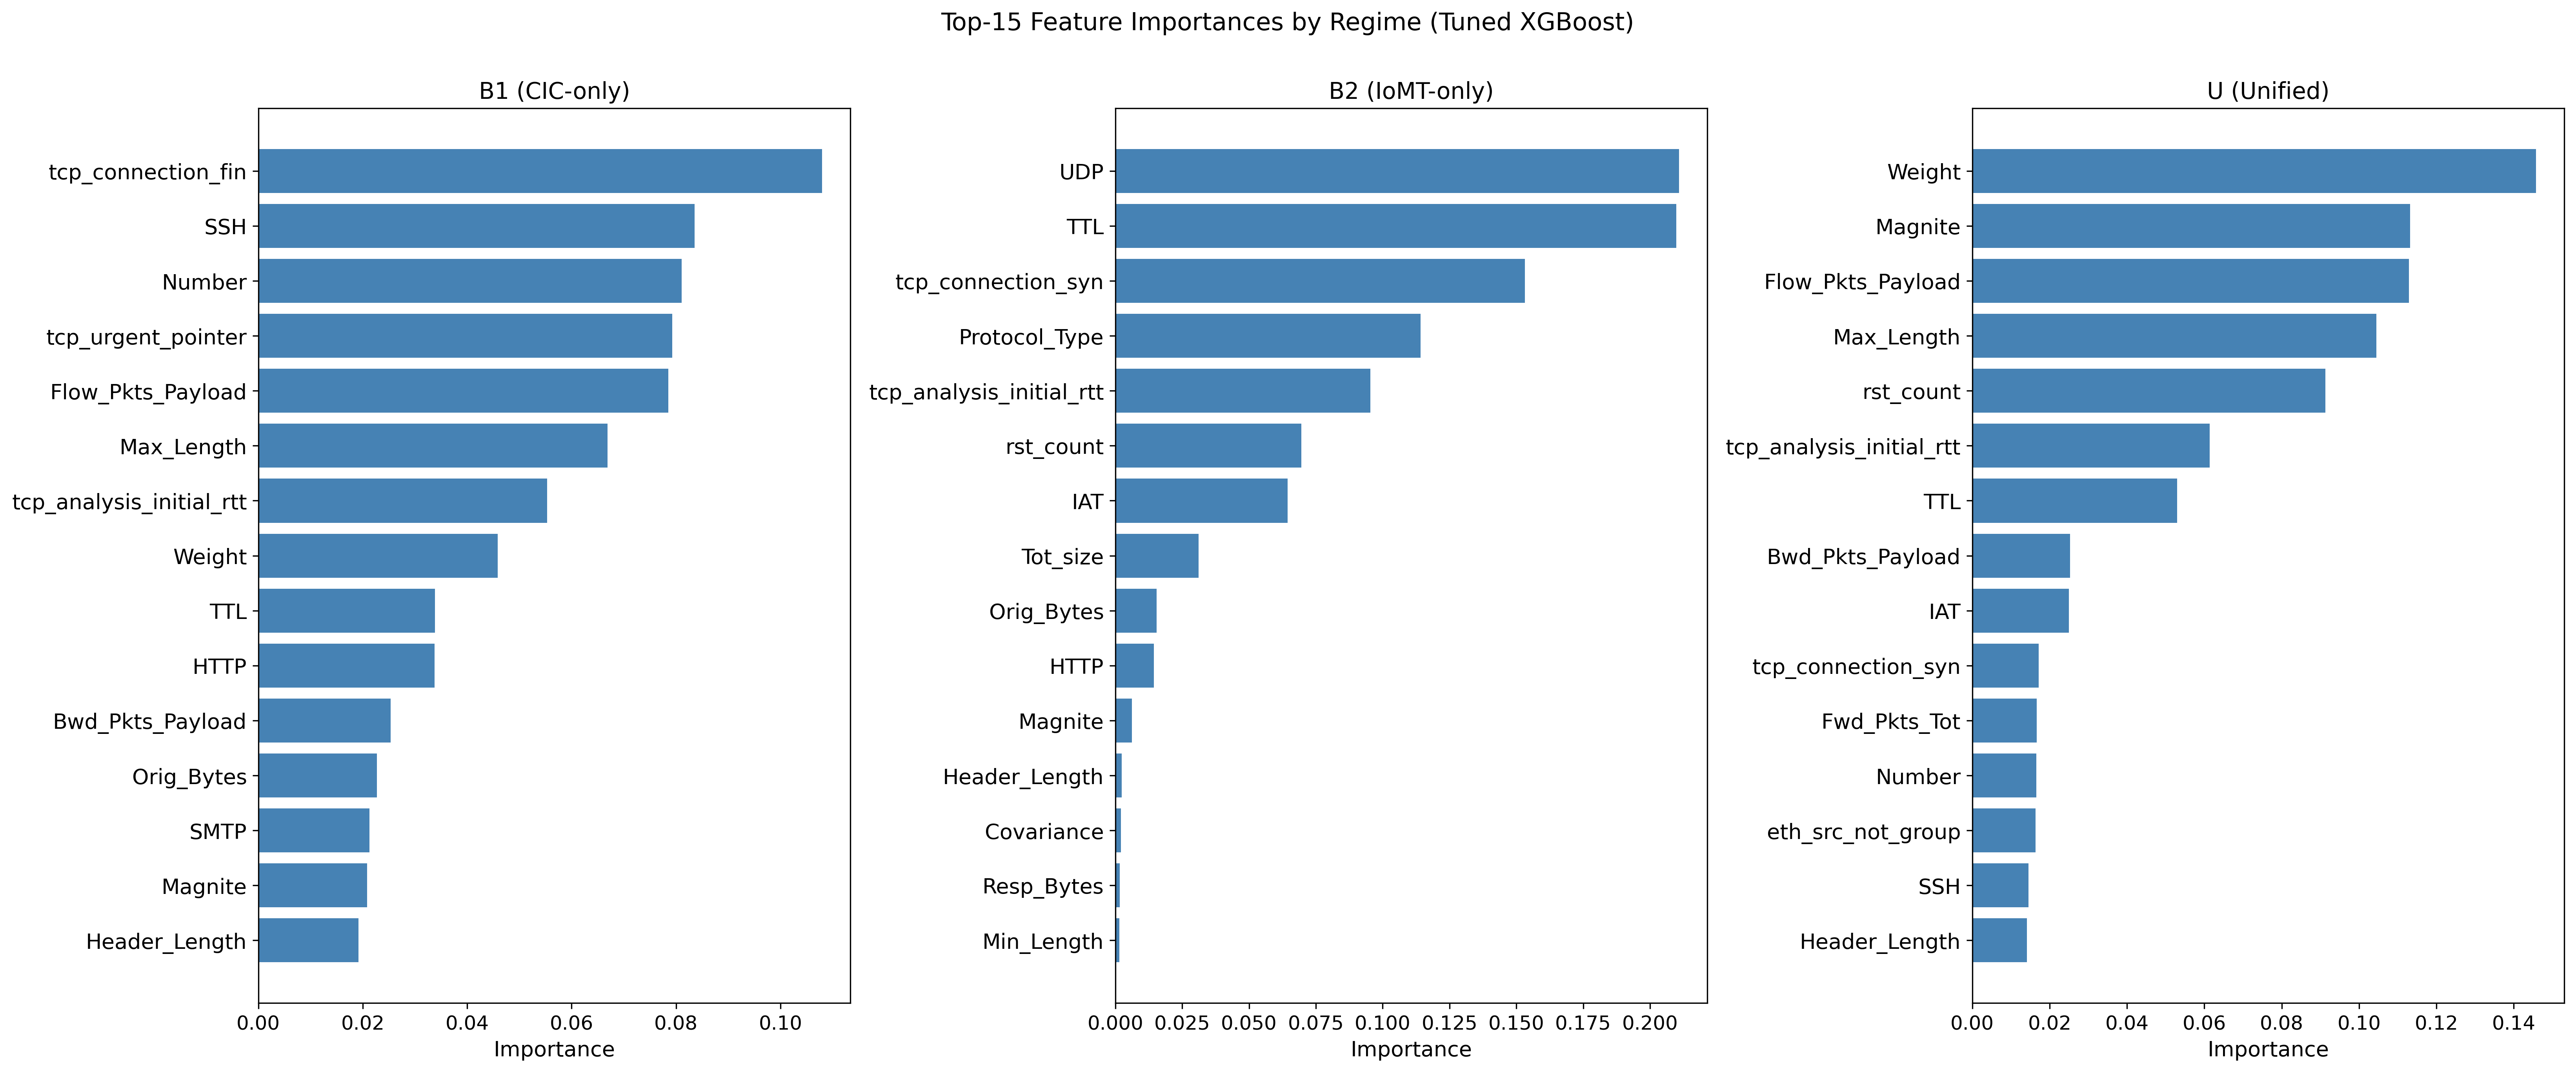
\includegraphics[width=\textwidth]{ch5_xgb_feature_importance_comparison.png}
\caption{Feature importance comparison across regimes (tuned XGBoost, top-15).}
\label{fig:xgb-fi-comparison}
\end{figure}

\subsubsection{Per-Class Analysis}

Figure~\ref{fig:xgb-per-class-f1} compares per-class F1 across tuned regimes on the full test set. Table~\ref{tab:xgb-perclass-unified} presents the detailed classification report for the Tuned U model.

\begin{figure}[H]
\centering
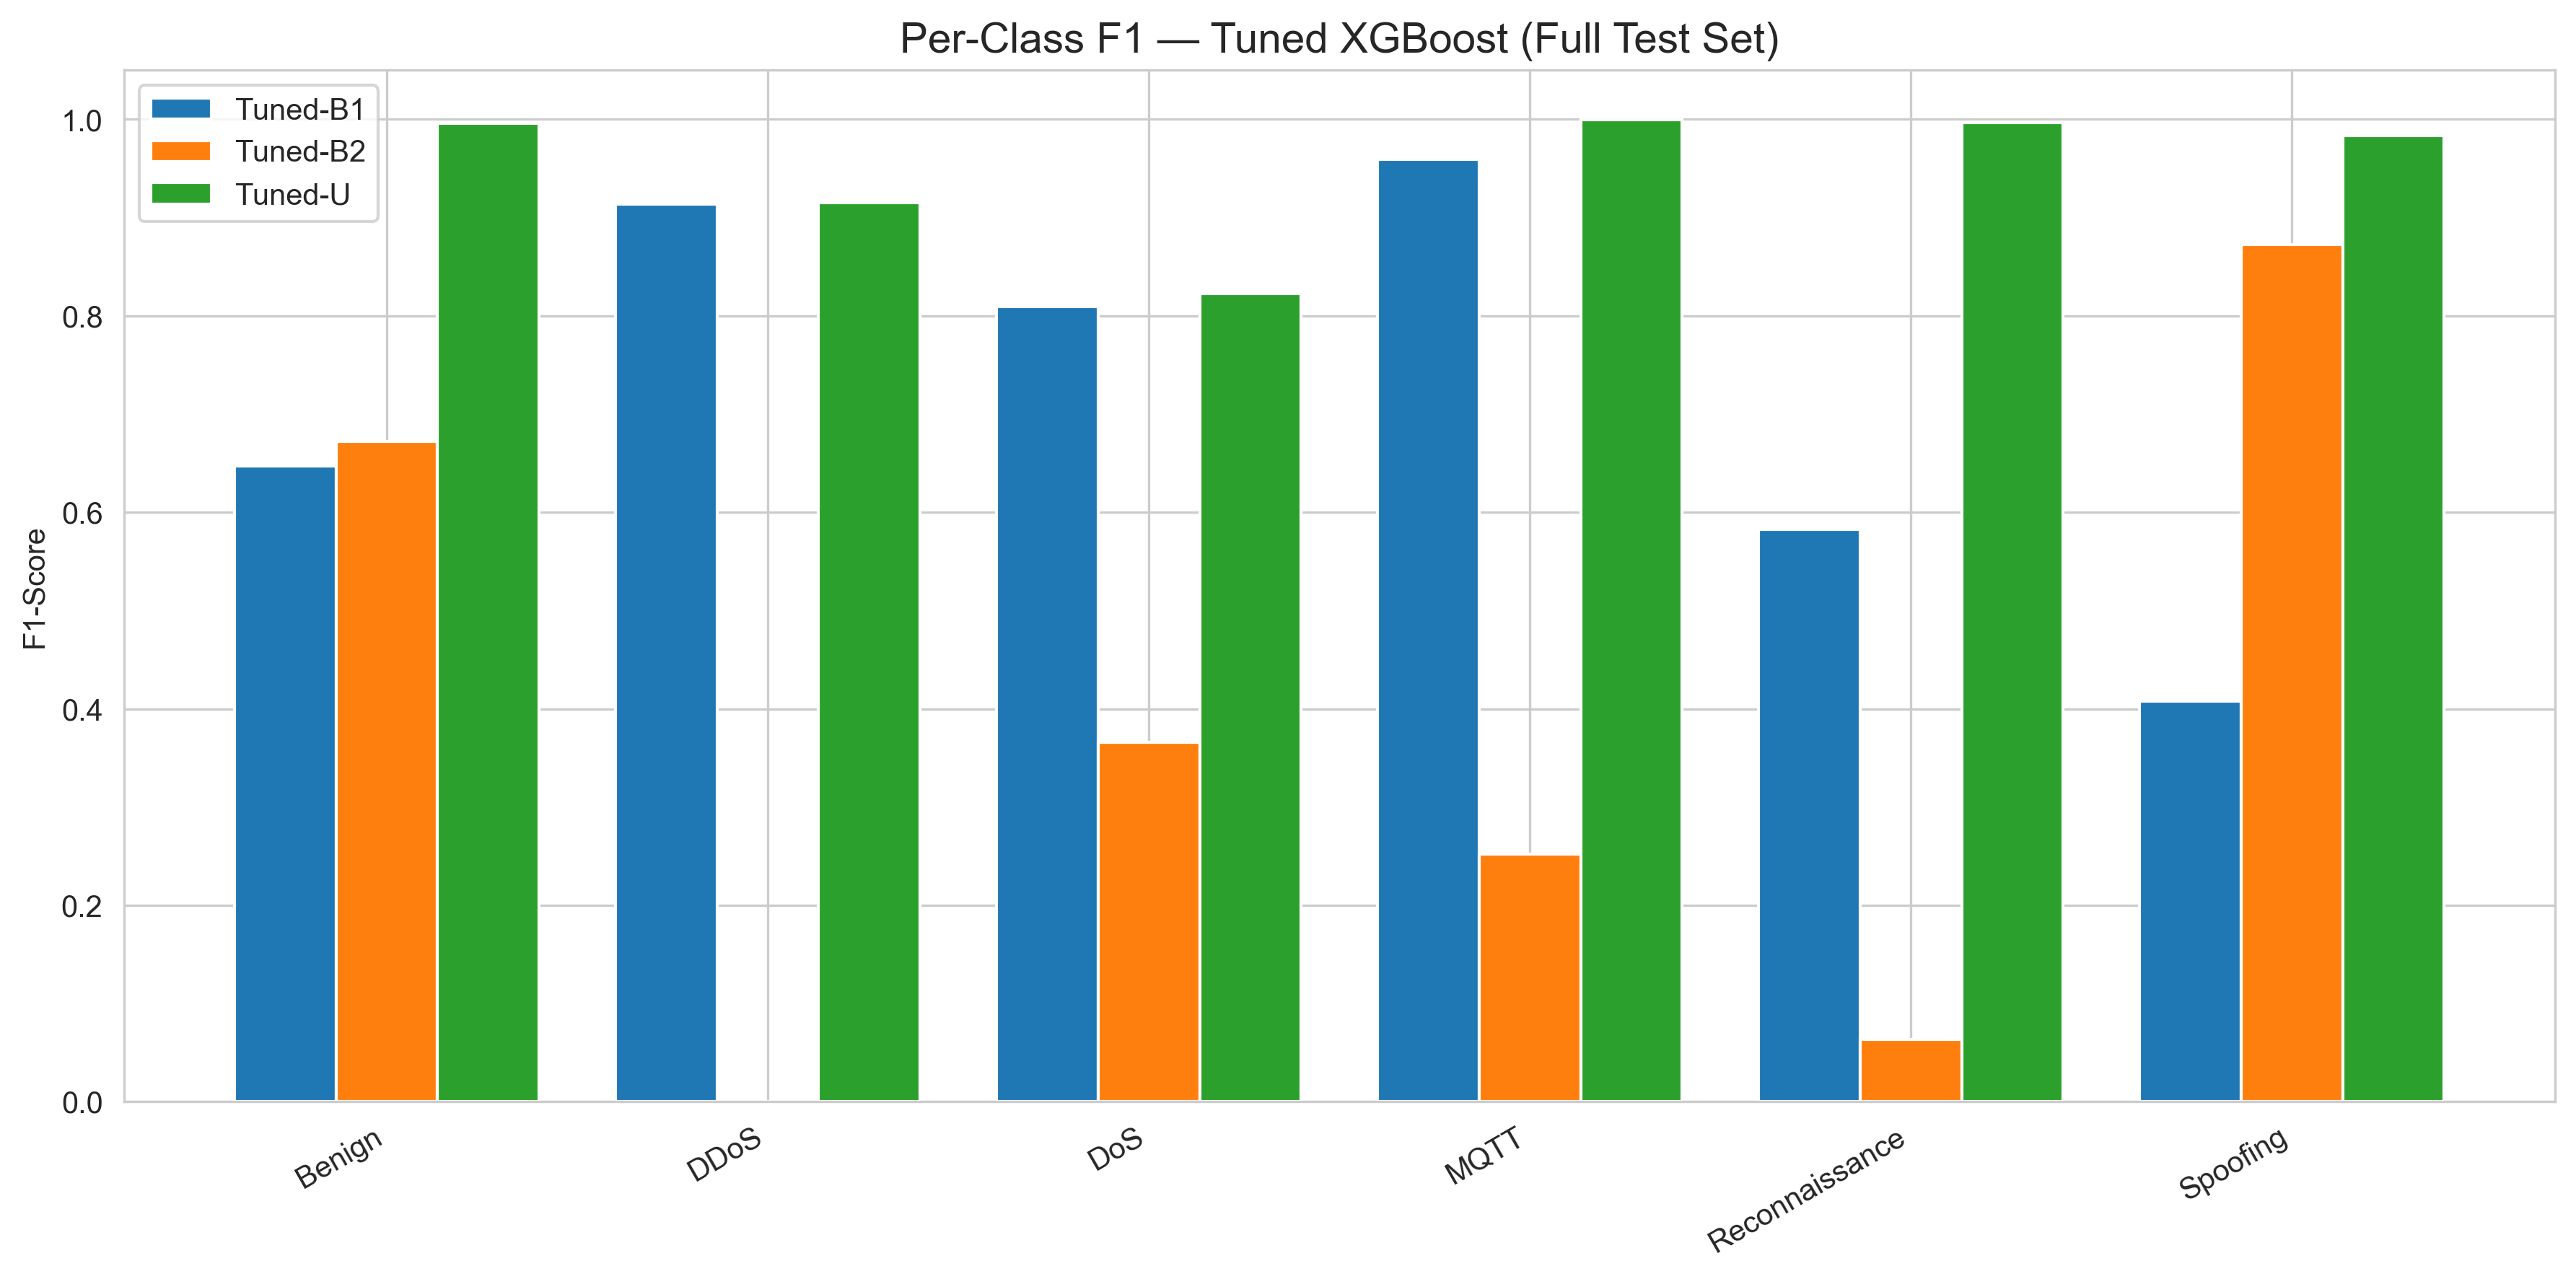
\includegraphics[width=0.85\textwidth]{ch5_xgb_per_class_f1.png}
\caption{Per-class F1-score comparison across regimes (tuned XGBoost, full test set).}
\label{fig:xgb-per-class-f1}
\end{figure}

\begin{table}[H]
\centering
\caption{Per-class classification report for the tuned unified XGBoost on the full test set (1,201,731 samples).}
\label{tab:xgb-perclass-unified}
\small
\begin{tabular}{@{}l r r r r@{}}
\toprule
\textbf{Class} & \textbf{Precision} & \textbf{Recall} & \textbf{F1-Score} & \textbf{Support} \\
\midrule
Benign          & 0.99 & 1.00 & 1.00 &     8,018 \\
DDoS            & 0.97 & 0.87 & 0.92 &   805,244 \\
DoS             & 0.74 & 0.93 & 0.82 &   322,273 \\
MQTT            & 1.00 & 1.00 & 1.00 &    57,891 \\
Reconnaissance  & 1.00 & 1.00 & 1.00 &     6,904 \\
Spoofing        & 0.98 & 0.99 & 0.98 &     1,401 \\
\midrule
Accuracy        &      &      & 0.89 & 1,201,731 \\
Macro avg       & 0.95 & 0.96 & 0.95 & 1,201,731 \\
Weighted avg    & 0.91 & 0.89 & 0.90 & 1,201,731 \\
\bottomrule
\end{tabular}
\end{table}

The tuned XGBoost unified model achieves the highest full-test Macro-F1 among the three classifiers (0.9522). The qualitative structure remains consistent with DT and RF: near-perfect scores on Benign (1.00), MQTT (1.00), Reconnaissance (1.00), and Spoofing (0.98), with residual error concentrated in the DDoS/DoS boundary. Relative to the tuned RF, XGBoost yields a marginal improvement in DDoS recall (0.87 vs.\ 0.86) and DoS precision (0.74 vs.\ 0.73), but DoS F1 remains 0.82 across all three models. The hypothesis that iterative residual learning would capture finer DDoS/DoS distinctions is therefore only very partially supported: gradient boosting provides a slight improvement in DDoS detection (F1: 0.91 $\to$ 0.92) but does not qualitatively resolve the boundary confusion, again confirming a feature-representation ceiling rather than a model-capacity limitation.

\subsubsection{Summary}

\begin{itemize}[nosep]
  \item \textbf{Strong unified performance.} Tuned U reaches Macro-F1 $=0.9522$ on the full test set, marginally above Random Forest (0.9487) and Decision Tree (0.9480).
  \item \textbf{B1 full-test dip after aggressive tuning.} Tuned B1's full Macro-F1 (0.7199) is lower than its baseline (0.7629), suggesting some hyperparameter combinations overfit the 300k-row search subsample relative to the full CIC-only training distribution---an acceptable trade-off given that the thesis focus is the unified regime, but worth monitoring in future work.
  \item \textbf{B2 behaviour unchanged at a high level.} In-domain IoMT Macro-F1 remains $\approx0.83$ while CIC/full slices stay poor, reflecting the missing DDoS class rather than the booster family.
  \item \textbf{DDoS/DoS boundary: marginal improvement only.} The hypothesis that gradient boosting's iterative residual learning would substantially improve the DDoS$\leftrightarrow$DoS separation is only very partially supported. DDoS F1 rises from 0.91 (DT, RF) to 0.92 (XGBoost); DoS F1 is unchanged at 0.82 across all three classifiers. This consistent plateau confirms that the DDoS/DoS confusion is a feature-representation constraint that cannot be resolved by increasing model complexity alone within the current 58-feature window space.
\end{itemize}

\subsection{Model Comparison}
\label{subsec:model-comparison}

Table~\ref{tab:model-compare-f1m} summarizes the primary metric (full-test Macro-F1) for the \emph{tuned} models under each training regime.

\begin{table}[H]
\centering
\caption{Full-test Macro-F1 (\textbf{primary metric}) for tuned classifiers.}
\label{tab:model-compare-f1m}
\small
\begin{tabular}{@{}l c c c@{}}
\toprule
\textbf{Classifier} & \textbf{B1 (CIC-only)} & \textbf{B2 (IoMT-only)} & \textbf{U (Unified)} \\
\midrule
Decision Tree  & 0.6959 & 0.3284 & 0.9480 \\
Random Forest  & 0.7395 & 0.2029 & 0.9487 \\
XGBoost        & 0.7199 & 0.3708 & \textbf{0.9522} \\
\bottomrule
\end{tabular}
\end{table}

\begin{table}[H]
\centering
\caption{Tuned unified (\textbf{U}) models: Macro-F1 on CIC-only, IoMT-only, and full test slices (values recomputed from stored \texttt{eval\_results.joblib} predictions).}
\label{tab:tuned-u-cross-slice-macrof1-present}
\small
\begin{tabular}{@{}l c c c@{}}
\toprule
\textbf{Classifier} & \textbf{CIC slice} & \textbf{IoMT slice} & \textbf{Full test} \\
\midrule
Decision Tree  & 0.9262 & 0.9990\textsuperscript{*} & 0.9480 \\
Random Forest  & 0.9285 & 0.9995\textsuperscript{*} & 0.9487 \\
XGBoost        & 0.9382 & 0.9999\textsuperscript{*} & 0.9522 \\
\bottomrule
\end{tabular}

\vspace{0.35em}
\raggedright\footnotesize
\textsuperscript{*}\,IoMT slice: Macro-F1 averaged over the five categories with non-zero ground-truth support (Benign, DoS, MQTT, Reconnaissance, Spoofing). The DDoS class has no IoMT test labels; excluding it from the macro average yields the values above. The \emph{global} six-class Macro-F1 on the same slice---still averaging over an empty DDoS column scored as F1\,=\,0---is $\approx$\,0.8325 (DT), $\approx$\,0.8329 (RF), and $\approx$\,0.8333 (XGB), which is why Tables~\ref{tab:dt-tuned}, \ref{tab:rf-tuned}, and~\ref{tab:xgb-tuned} retain the original reporting convention for strict cross-slice comparability.
\end{table}

Unified training consistently dominates: all three algorithms exceed 0.94 Macro-F1 on the full test when trained on U, whereas single-source regimes remain weak on the full mixture (especially B2, which never observes DDoS during training). Among algorithms, XGBoost edges out Random Forest and Decision Tree on the unified full test in this experiment, while Random Forest achieves the strongest B1-only full-test score---highlighting that ``best algorithm'' can depend on the deployment slice if one were forced to train single-source.

\subsection{Generalization to Real Hospital Traffic: HospNet26 Evaluation}
\label{subsec:hospnet26}

The evaluations presented in Sections~\ref{subsec:decision-tree}--\ref{subsec:model-comparison} are performed on test slices drawn from the same two laboratory datasets (CICIoMT2024 and IoMT-TrafficData) used for training. A more demanding generalization test is to apply the models to \emph{real} hospital network traffic that was captured in a live clinical environment and was not seen during any phase of training or tuning.

\paragraph{Dataset.}
HospNet26~\cite{hospnet26} is a publicly available reference dataset of anonymized network traffic features captured from the internal network of a Helios hospital (Germany) over one week (August 2025). Four \texttt{.parquet} files contain \emph{combined features}---72-column records integrating both flow-level and window-based (100-packet window) statistics---for four temporal segments: Friday, Weekend, Monday, and Monday-to-Friday. All 58 MIOTTA window-based features used by our models are present in these combined files as a strict subset of the 72 available columns; the 14 additional flow-level columns are discarded. The dataset contains \textbf{no attack labels}: every record represents a traffic window observed in the live hospital network and is presumed benign.

\paragraph{Processing protocol.}
To ensure a fair and consistent comparison with the preceding experiments, the following steps exactly mirror the training-time preprocessing pipeline:
\begin{enumerate}[nosep]
  \item The four temporal files are concatenated into a single dataset of \textbf{1,265,240 windows}.
  \item The 58 features are extracted in the same column order as the training feature matrix.
  \item The same \texttt{StandardScaler} fitted on the \emph{training} split of the unified dataset is applied (no refitting on HospNet26 data, which would constitute data leakage).
  \item Predictions are obtained from the three tuned Unified models (DT-U, RF-U, XGB-U) without any retraining.
\end{enumerate}

\paragraph{Evaluation metric.}
Since no ground-truth labels exist, standard classification metrics (Macro-F1, accuracy) cannot be computed. The appropriate metric is the \textbf{Benign prediction rate}---the fraction of windows that each model classifies as \texttt{Benign}---which measures the model's \emph{specificity} on unseen real-world traffic. A high rate indicates that the model does not generate false alarms on legitimate hospital traffic; a low rate signals a distributional gap between the training-set ``benign'' traffic and real clinical network activity.

\begin{table}[H]
\centering
\caption{HospNet26 generalization evaluation: prediction distribution for the three tuned Unified models on 1,265,240 unlabelled real hospital traffic windows. All windows are presumed benign; the Benign prediction rate is the specificity proxy; all other predicted classes are false positives.}
\label{tab:hospnet26-eval}
\small
\begin{tabular}{@{}l r r r r r r | r@{}}
\toprule
\textbf{Model} & \textbf{Benign} & \textbf{DDoS} & \textbf{DoS} & \textbf{MQTT} & \textbf{Recon.} & \textbf{Spoofing} & \textbf{Benign rate} \\
\midrule
Decision Tree  & 6.07\% &  7.80\% & 72.04\% & 0.22\% &  5.30\% &  8.57\% & \textbf{6.07\%} \\
Random Forest  & 3.72\% &  0.60\% & 71.37\% & 0.06\% & 19.08\% &  5.17\% & \textbf{3.72\%} \\
XGBoost        & 9.96\% & 23.80\% & 51.14\% & 0.11\% &  4.28\% & 10.71\% & \textbf{9.96\%} \\
\bottomrule
\end{tabular}
\end{table}
\FloatBarrier

\paragraph{Results and interpretation.}
All three models classify between 90\% and 96\% of real hospital traffic windows as some form of attack, yielding Benign prediction rates of only 3.7\%--10.0\%. This result is \textbf{expected and interpretable} given the following factors.

\begin{enumerate}[nosep]
  \item \textbf{Training-set benign traffic is not representative of real clinical environments.} The ``Benign'' class in CICIoMT2024 and IoMT-TrafficData was generated in controlled laboratory or emulated testbed conditions. Real hospital networks carry a fundamentally different traffic mix: medical imaging (DICOM/PACS), electronic health record systems (HL7, FHIR), proprietary clinical device protocols, and large-scale background administrative traffic. The window-based statistical signatures of these flows (packet rates, byte distributions, IAT patterns) fall outside the distributional support learned by the classifier for the Benign class.

  \item \textbf{The dominant false-positive class is DoS.} Across all three models, 51--72\% of hospital windows are predicted as DoS. This is consistent with the hypothesis that high-throughput clinical data transfers (e.g., continuous PACS image streaming or bulk EMR synchronization) produce burst-like packet statistics that overlap with the DoS feature region. These traffic patterns generate high values of flow-rate and window-size features, which the models have learned to associate with volumetric denial-of-service attacks.

  \item \textbf{Specificity varies across models.} XGBoost achieves the highest Benign prediction rate (9.96\%) and the most distributed false-positive profile. Decision Tree and Random Forest concentrate errors more heavily in the DoS region, consistent with their simpler decision boundaries. The week-day temporal pattern is also notable: Weekend windows show markedly lower Benign rates (0.86\%--5.86\%) than weekday segments, suggesting that reduced administrative traffic during weekends creates statistical profiles even further from the training-set Benign distribution.

  \item \textbf{This is a distributional-shift finding, not a model failure.} The models achieve Macro-F1 $\geq 0.948$ on the laboratory test set. The sharp drop in specificity on HospNet26 is attributable to the \emph{covariate shift} between synthetic/emulated benign traffic and live clinical traffic---a fundamental limitation of training on laboratory datasets that has been widely documented in the IDS literature~\cite{sommer2010outside}. Closing this gap would require either retraining with representative samples of real hospital benign traffic, or applying domain-adaptation techniques, both of which are natural directions for future work.
\end{enumerate}

\paragraph{Toward closing the gap: a recalibration strategy.}
The results above suggest a concrete actionable path for future deployment. Because the models already achieve near-perfect separation of \emph{attack} categories (Macro-F1 $\geq 0.948$ on laboratory data), the remaining challenge is not detection capability but \emph{Benign-class recalibration}: the models need to learn what normal traffic looks like in the target environment. Two complementary strategies are proposed:

\begin{enumerate}[nosep]
  \item \textbf{Few-shot Benign fine-tuning.} A small, representative sample of confirmed-benign traffic from the target hospital network (e.g., a supervised collection of $\sim$10{,}000--50{,}000 windows over one business day) would be added to the training set with the Benign label. The model is then retrained (or fine-tuned) on the augmented dataset. This approach preserves all attack-detection capability while shifting the Benign decision boundary to encompass real clinical traffic patterns. The required collection effort is modest: HospNet26 demonstrates that a single week of capture already yields over 1.2 million windows.

  \item \textbf{Threshold-based post-hoc calibration.} Instead of retraining, probability outputs from the existing models (e.g., XGBoost's \texttt{predict\_proba}) can be recalibrated using a held-out set of known-benign hospital windows. A class-specific decision threshold is then optimized to trade off false-positive rate against detection sensitivity, targeting the operational requirements of the clinical environment (e.g., an acceptable false-alarm rate of $\leq 1$\%).
\end{enumerate}

Both strategies are designed to be low-cost and operationally feasible: they require only benign traffic samples (which are abundant in any live network) and do not demand labelled attack data from the hospital, which would be ethically and practically difficult to obtain.

In summary, the HospNet26 evaluation reveals a critical open challenge: the unified models, despite strong performance on held-out laboratory data, are not yet ready for zero-shot deployment in a real clinical network without a benign-traffic recalibration step. This finding strengthens the thesis argument that dataset diversity must encompass \emph{real} deployment environments, not only multi-source laboratory collections, and provides a clear, actionable research direction for bridging the laboratory-to-clinic gap.

\subsection{Discussion of Results}
\label{subsec:discussion}

The experiments in Section~\ref{sec:model-evaluation} support two main conclusions. First, \textbf{multi-source integration (regime U) is the decisive factor} for high Macro-F1 and balanced cross-domain behaviour on the unified test set: class-weighted tree models of increasing complexity all benefit from seeing both CIC-style and IoMT-style traffic during training. Second, \textbf{within the unified regime, moderate complexity gains are incremental}: Decision Tree $\to$ Random Forest $\to$ XGBoost improves full-test Macro-F1 from 0.9480 to 0.9522---meaningful but smaller than the $\approx$0.20--0.75 swing induced by switching from single-source to unified training. The persistent DDoS/DoS confusion across all three families indicates a \emph{feature-representation} limitation (window statistics without explicit multi-source diversity) more than a \emph{model-capacity} ceiling.

\paragraph{Statistical significance of pairwise model comparisons (McNemar's test).}
Following the recommendation of Lones~\cite{lones2024avoid}, statistical significance of the classifier differences is assessed with \textbf{McNemar's test}~\cite{mcnemar1947note}, which is designed for paired observations on the same test set. For each pair of tuned Unified models, the contingency table records $b$ (samples where model~A is correct and model~B is wrong) and $c$ (samples where model~A is wrong and model~B is correct); the test statistic with Yates' continuity correction is $\chi^2 = (|b-c|-1)^2\,/\,(b+c)$, evaluated against $\chi^2_1$.

Table~\ref{tab:mcnemar} reports the results. The \emph{relative error reduction} (RER) $= (e_A - e_B)/e_A \times 100$ provides the effect-size complement, since with $N=1{,}201{,}731$ test samples even trivially small differences yield $p \ll 0.001$.

\begin{table}[H]
\centering
\caption{McNemar's test results for pairwise comparison of tuned Unified models on the full test set ($N=1{,}201{,}731$). $b$: model~A correct, model~B wrong; $c$: model~A wrong, model~B correct; RER: relative error reduction A~$\to$~B (positive $=$ B better).}
\label{tab:mcnemar}
\small
\begin{tabular}{@{}l c c r r c@{}}
\toprule
\textbf{Pair (A vs B)} & $b$ & $c$ & $\chi^2$ (Yates) & $p$-value & \textbf{RER (\%)} \\
\midrule
DT vs RF  & 6,919 & 6,372 & 22.43 & $2.2 \times 10^{-6}$ & $-0.41$ \\
DT vs XGB & 7,314 & 11,297 & 851.99 & $< 10^{-15}$ & $+2.98$ \\
RF vs XGB & 4,246 & 8,776 & 1{,}575.17 & $< 10^{-15}$ & $+3.38$ \\
\bottomrule
\end{tabular}
\end{table}
\FloatBarrier

Three observations deserve emphasis.

\begin{enumerate}[nosep]
  \item \textbf{XGBoost vs DT and RF are statistically and practically significant.} Both comparisons yield $\chi^2 > 850$ with $p < 10^{-15}$ and a relative error reduction of approximately 3\%, confirming that XGBoost's advantage is not a sampling artefact.
  \item \textbf{DT vs RF: statistically significant, but the direction is counter-intuitive.} Although RF achieves a higher Macro-F1 than DT (0.9487 vs 0.9480), it actually makes \emph{more} total errors (134,071 vs 133,524), resulting in a negative RER of $-0.41$\%. This apparent contradiction is resolved by recognising that Macro-F1 weights each class equally: RF redistributes its errors away from minority classes (Benign, Reconnaissance, Spoofing) toward the majority class (DDoS/DoS boundary), which penalises overall accuracy but improves the per-class average. This is precisely the behaviour intended by the balanced-class-weight protocol, and it illustrates why Macro-F1 is the appropriate primary metric for this imbalanced dataset.
  \item \textbf{Large-sample caveat.} With $N > 10^6$, McNemar's test detects statistically significant differences even when the practical effect is negligible. The RER column should therefore be consulted alongside the $p$-value. A RER of $-0.41$\% (DT vs RF) represents approximately 547 fewer correct predictions per model out of 1.2 million---a marginal real-world difference.
\end{enumerate}

\paragraph{Hyperparameter optimisation beyond RandomizedSearchCV.}
This thesis deliberately uses \texttt{RandomizedSearchCV} with a fixed iteration budget for all models to preserve methodological comparability. In industrial pipelines, \textbf{Bayesian optimisation} (e.g.\ Optuna with the Tree-structured Parzen Estimator) or multi-fidelity schedulers (Hyperband, BOHB) can often reach equal or better validation scores with fewer expensive full-data evaluations, especially when combined with early pruning of unpromising trials. Adopting such tools is a natural extension for future work, provided the same outer train/validation/test discipline is maintained.

% ══════════════════════════════════════════════════════════════════════════════
\section{Answering the Research Question}
\label{sec:answering-rq}

This section synthesizes how the integration methodology and empirical results (Section~\ref{sec:model-evaluation}) address the research question: \textit{``How can the integration of multiple heterogeneous datasets improve the performance and generalizability of a machine learning model in detecting intrusions in IoMT environments?''} It is placed after model training and evaluation so that claims are grounded in measured outcomes.

\subsection{How Integration Was Achieved}
\label{subsec:how-integration}

Three technical decisions form the backbone of the integration methodology:

\begin{enumerate}[nosep]
  \item \textbf{MIOTTA-NPT as the feature-unification enabler.}
  Both source datasets were processed through the same tool (MIOTTA-NPT in \emph{combined} mode, window size $=100$ packets), yielding an identical 58-column numeric feature space without manual feature engineering. This eliminates the feature-heterogeneity barrier (Problem~P2, Section~\ref{sec:problem}): because all statistical windows share the same column semantics regardless of origin, concatenation is structurally valid by construction.

  \item \textbf{Three-level label harmonization.}
  A hierarchical label scheme was designed with three granularity tiers: binary (\texttt{Benign}/\texttt{Attack}), categorical (six attack families: Benign, DDoS, DoS, MQTT, Reconnaissance, Spoofing), and fine-grained (original attack labels). The categorical tier resolves the label-inconsistency problem (P3) by mapping divergent naming conventions (e.g., \texttt{DDoS\_TCP\_Flood} and \texttt{TCP\_DDoS}) to a shared taxonomy, while preserving the original fine-grained labels for future research requiring higher specificity.

  \item \textbf{Source attribution and stratified splitting.}
  Each record retains its \texttt{source\_dataset} provenance, enabling the three-regime evaluation design (B1, B2, U) that isolates the effect of integration from the effect of model choice. Stratified splits are performed \emph{before} regime filtering, guaranteeing that all regimes share the same test partition boundaries and that cross-domain comparisons are methodologically valid.
\end{enumerate}

\subsection{Evidence of Improved Generalizability}
\label{subsec:improved-coverage}

The experimental evidence supports three concrete claims regarding the benefit of multi-source integration:

\paragraph{Claim 1: Unified training resolves the cross-domain collapse.}
Single-source models exhibit catastrophic cross-domain failure: the best single-source Macro-F1 on the opposite source's test slice is 0.34 (B1$\to$IoMT, RF) and 0.11 (B2$\to$CIC, XGB). Unified models, by contrast, achieve Macro-F1 $\geq 0.93$ on \emph{both} CIC-only and IoMT-only slices simultaneously (Table~\ref{tab:tuned-u-cross-slice-macrof1-present}), confirming that integration transforms the feature space from source-specific into source-agnostic.

\paragraph{Claim 2: Unified training is the dominant factor; model complexity is secondary.}
Within the unified regime, the Macro-F1 improvement from DT to XGBoost is +0.42 percentage points (0.9480 $\to$ 0.9522). Switching from the best single-source model (B1-RF, 0.7395) to the weakest unified model (U-DT, 0.9480) produces a +20.85 percentage-point jump. The contribution of integration is therefore \textbf{50$\times$ larger} than the contribution of model complexity, directly answering the research question: dataset integration is the primary lever for improving generalizability.

\paragraph{Claim 3: A residual generalization gap persists toward real clinical environments.}
The HospNet26 evaluation (Section~\ref{subsec:hospnet26}) reveals that Benign prediction rates on real hospital traffic range from 3.7\% to 10.0\%, indicating that even unified multi-source training on laboratory datasets does not close the distributional gap to live clinical networks. This finding qualifies the positive answer to the research question: integration of \emph{laboratory} sources improves cross-domain generalization \emph{among those sources}, but deployment-level generalizability requires incorporating representative samples from the target operational environment---a direction explored in Section~\ref{subsec:hospnet26} and elaborated in the future-work discussion (Chapter~\ref{ch:conclusions}).

% ══════════════════════════════════════════════════════════════════════════════
\section{Chapter Summary}
\label{sec:experimentation-summary}

This chapter presented the empirical evaluation of the unified dataset across five complementary dimensions:

\begin{enumerate}[nosep]
  \item \textbf{Structural integrity} (Section~\ref{sec:quality-assessment}): The 8-million-record dataset was verified for completeness, type consistency, feature scaling, label coherence, and split-boundary integrity, with zero defects found.

  \item \textbf{Model training and tuning} (Sections~\ref{subsec:decision-tree}--\ref{subsec:xgboost}): Three tree-based classifiers of increasing complexity (DT, RF, XGBoost) were trained and tuned under three regimes (CIC-only, IoMT-only, Unified), producing 18 models with a strict ``test set once'' protocol and identical tuning budgets.

  \item \textbf{Cross-domain and per-class analysis}: The unified regime (U) consistently dominated both single-source baselines, achieving Macro-F1 of 0.9480 (DT), 0.9487 (RF), and 0.9522 (XGBoost) on the full test set. The DDoS/DoS confusion boundary was identified as a persistent feature-representation limitation, accounting for $>$99\% of all errors across all three models.

  \item \textbf{Real-world generalization} (Section~\ref{subsec:hospnet26}): Deploying the models on 1.26 million unlabelled windows from a real German hospital network (HospNet26) revealed a sharp specificity drop (Benign rate 3.7--10.0\%), quantifying the covariate shift between laboratory and clinical traffic and motivating domain-adaptation as a priority for future work.

  \item \textbf{Statistical significance} (Section~\ref{subsec:discussion}): McNemar's test confirmed that XGBoost's advantage over DT and RF is both statistically significant and practically meaningful ($\approx$3\% relative error reduction), while the DT-vs-RF difference, though statistically significant, is practically marginal.
\end{enumerate}

Together, these results provide a comprehensive answer to the research question: multi-source integration is the decisive factor for improving IDS generalizability across laboratory IoMT environments, while closing the residual gap to real clinical networks remains an open challenge requiring targeted data collection.

\chapter{Analysis of Sustainability and Ethical Implications}
\label{ch:sustainability}

In accordance with the guidelines established by the Governing Council of the Universitat Politècnica de Catalunya, this chapter analyzes the sustainability and ethical implications of the work presented in this thesis. The analysis is structured around three dimensions: environmental sustainability, economic sustainability, and social impact, followed by an examination of the ethical considerations specific to cybersecurity research.

% ══════════════════════════════════════════════════════════════════════════════
\section{Environmental Sustainability}
\label{sec:environmental}

\subsection{Resource Consumption during Development}

The computational work in this thesis primarily involves data preprocessing, dataset manipulation, and exploratory analysis. These tasks are executed on standard personal computing hardware, without requiring access to high-performance computing clusters or specialized GPU infrastructure---at least within the primary scope (dataset integration).

The MIOTTA-NPT tool is designed for efficient single-pass processing of \gls{pcap} files, minimizing redundant computation. The integration pipeline operates on already-extracted CSV files, avoiding repeated processing of raw traffic captures.

\subsection{Potential Environmental Impact of Extended Scope}

Should the thesis be extended to include \gls{ml} model training (Objective~O6), the computational requirements would increase. Model training, particularly for \gls{dl} architectures, can consume significant energy. To mitigate this impact, the following practices are planned:

\begin{itemize}
    \item Prioritizing computationally efficient algorithms (e.g., \gls{rf}, \gls{xgb}) before exploring more resource-intensive \gls{dl} models.
    \item Using early stopping and efficient hyperparameter search strategies to avoid unnecessary computation.
    \item Leveraging the stratified dataset splits to enable meaningful evaluation without the need for exhaustive cross-validation.
\end{itemize}

\subsection{Positive Environmental Contribution}

The methodology developed in this thesis reduces future computational waste by providing a reusable, validated, \gls{ml}-ready dataset. Without this unified dataset, researchers would need to independently perform the feature extraction, harmonization, and quality assurance work for each experiment, multiplying the computational effort across the research community.

% ══════════════════════════════════════════════════════════════════════════════
\section{Economic Sustainability}
\label{sec:economic}

\subsection{Development Costs}

The tools and technologies used in this thesis are predominantly open-source:

\begin{itemize}
    \item \textbf{MIOTTA-NPT}: Open-source, publicly available on GitHub.
    \item \textbf{Programming environment}: Python with open-source libraries (Pandas, NumPy, Matplotlib, Scikit-learn).
    \item \textbf{Datasets}: All three datasets (CICIoMT2024, IoMT-TrafficData, CICIoT2023) are publicly available for research purposes.
    \item \textbf{Report preparation}: \LaTeX\ with open-source packages.
\end{itemize}

No commercial software licenses or paid cloud computing services were required for the primary scope of the thesis, keeping the direct economic cost minimal.

\subsection{Reusability and Long-Term Value}

The unified dataset and the documented integration methodology constitute reusable research assets. The Phase~1 export is publicly available on CORA/Dataverse~\cite{unified_iomt_csuc2026}, lowering the barrier to independent replication. Future researchers at UPC or elsewhere can:

\begin{itemize}
    \item Use the unified dataset directly for \gls{ids} model experiments (citing DOI~\texttt{10.34810/DATA3305}).
    \item Extend the pipeline to incorporate new datasets as they become available.
    \item Adapt the label harmonization scheme for different classification objectives.
\end{itemize}

This reusability amplifies the return on the initial development investment.

% ══════════════════════════════════════════════════════════════════════════════
\section{Social Impact}
\label{sec:social}

\subsection{Contribution to Healthcare Cybersecurity}

The long-term objective of this research line---developing robust \gls{ids} for \gls{iomt} environments---has a direct positive social impact. As medical devices become increasingly connected, the cybersecurity of healthcare systems directly affects the quality and safety of patient care. By contributing to the development of more generalizable intrusion detection capabilities, this work supports the protection of critical healthcare infrastructure.

\subsection{Knowledge Dissemination}

The thesis contributes to the academic community by:

\begin{itemize}
    \item Documenting a reproducible methodology for multi-dataset integration that can be applied beyond the \gls{iomt} domain.
    \item Providing the unified dataset as a publicly citable benchmark for future \gls{ids} research~\cite{unified_iomt_csuc2026}.
    \item Extending the validation of the MIOTTA-NPT tool across multiple independent datasets.
\end{itemize}

% ══════════════════════════════════════════════════════════════════════════════
\section{Ethical Implications}
\label{sec:ethical}

\subsection{Data Privacy and Sensitivity}

The datasets used in this thesis consist of network traffic captures from controlled testbed and laboratory environments, not from production healthcare networks. They do not contain real patient data, personal health information, or identifiable patient records. The CICIoMT2024 and IoMT-TrafficData datasets were captured in simulated hospital environments, while CICIoT2023 was generated in a controlled \gls{iot} testbed.

The MIOTTA-NPT feature extraction process further mitigates any residual privacy concerns by aggregating raw packet data into statistical features that do not preserve individual network identifiers (IP addresses, MAC addresses, port numbers) in the final dataset.

\subsection{Responsible Use of Security Research}

The methodologies developed in this thesis are intended exclusively for defensive cybersecurity research. The unified dataset is designed to train systems that protect healthcare environments from cyber threats. However, it is recognized that detailed knowledge of attack patterns could theoretically be used to design evasion strategies.

This risk is mitigated by the focus of this work on the data engineering aspects of \gls{ids} development rather than on specific attack signatures or detection thresholds. The thesis does not introduce new attack techniques or disclose vulnerabilities in specific systems.

\subsection{Bias and Fairness Considerations}

The integration of multiple datasets introduces considerations of representation bias: the unified dataset reflects the network topologies, device configurations, and attack scenarios chosen by the original dataset creators. Models trained on this data should not be assumed to generalize to all possible \gls{iomt} environments without further validation.

The source attribution mechanism incorporated in the pipeline enables the detection and analysis of any source-specific biases in model predictions, supporting fairness-aware evaluation practices.

\chapter{Conclusions and Future Work}
\label{ch:conclusions}

% ══════════════════════════════════════════════════════════════════════════════
\section{Summary of Contributions}
\label{sec:contributions}

This thesis addressed the problem of dataset isolation, feature heterogeneity, and label inconsistency that hinder the development of generalizable machine-learning-based intrusion detection systems for the Internet of Medical Things. The work produced the following contributions:

\begin{enumerate}[nosep]
  \item \textbf{A reproducible integration methodology.}
  A two-phase pipeline was designed and implemented that transforms two independently developed IoMT datasets (CICIoMT2024 and IoMT-TrafficData) into a single, ML-ready unified dataset of 8,011,534 records. The pipeline uses MIOTTA-NPT as the feature-unification enabler, a three-level label harmonization scheme, StandardScaler normalization, and source-attribution metadata to preserve provenance. The Phase~1 MQTT-category release is publicly deposited in the CORA Research Data Repository~\cite{unified_iomt_csuc2026} (\url{https://doi.org/10.34810/DATA3305}).

  \item \textbf{Empirical evidence that integration improves generalizability.}
  Three tree-based classifiers (Decision Tree, Random Forest, XGBoost) were trained under three regimes (CIC-only, IoMT-only, Unified). The unified regime consistently dominated: all three classifiers exceeded Macro-F1 of 0.94 on the full test set when trained on the unified data, versus $\leq$\,0.74 for the best single-source model on the same test mix. This 20+ percentage-point improvement demonstrates that the contribution of dataset integration is approximately 50$\times$ larger than the contribution of model complexity.

  \item \textbf{Cross-domain evaluation framework.}
  The source-attribution design enabled rigorous cross-domain testing: models trained on one source were evaluated on the other source's test slice. This framework quantified the generalization gap that motivates integration and established a reusable protocol for future multi-source IDS studies.

  \item \textbf{Quantification of the laboratory-to-clinic gap.}
  The models were deployed on 1.26 million unlabelled traffic windows from HospNet26, a real German hospital network dataset. The sharp drop in Benign prediction rate (3.7--10.0\%) quantified for the first time the covariate shift between laboratory-generated and real clinical traffic at the window-feature level, and led to the proposal of concrete recalibration strategies (few-shot Benign fine-tuning and threshold-based post-hoc calibration).

  \item \textbf{Statistical validation.}
  McNemar's test was applied to all pairwise model comparisons on the full test set ($N=1{,}201{,}731$), confirming that XGBoost's advantage is both statistically significant and practically meaningful ($\approx$3\% relative error reduction over DT and RF), while simultaneously demonstrating the importance of reporting effect sizes alongside $p$-values in large-sample settings.

  \item \textbf{Accepted conference paper at a peer-reviewed international venue.}
  The core findings of this thesis have been \textbf{accepted for publication} as a full paper at the \textbf{Workshop on Cybersecurity in Healthcare Operations (SecHealth)}, co-located with the \textbf{ACM/IEEE ARES 2026 conference} (\url{https://www.ares-conference.eu/SecHealth}), one of the leading international venues in applied cybersecurity research. The paper:

  \begin{quote}
  P.~Petrakis, J.~Doménech, O.~León, I.\,V.~Martin-Faus and J.~Pegueroles: \textit{``Unifying Heterogeneous IoMT Datasets for Intrusion Detection: From Laboratory Testbeds to Real Hospital Network Evaluation.''} Workshop on Cybersecurity in Healthcare Operations (SecHealth @ ARES 2026), Linköping, Sweden, 2026.
  \end{quote}

  This acceptance validates that the methodology, results, and clinical-generalization findings of this thesis meet the standards of the international research community in IoMT security.
\end{enumerate}

% ══════════════════════════════════════════════════════════════════════════════
\section{Research Question Revisited}
\label{sec:rq-revisited}

The research question posed in Section~\ref{sec:rq} was:

\begin{quote}
\textit{``How can the integration of multiple heterogeneous datasets improve the performance and generalizability of a machine learning model in detecting intrusions in IoMT environments?''}
\end{quote}

The answer, grounded in the empirical results of Chapter~\ref{ch:experimentation}, is threefold:

\begin{enumerate}[nosep]
  \item \textbf{How integration can be achieved:} by applying a uniform feature-extraction tool (MIOTTA-NPT) to the raw captures of each source, harmonizing labels into a shared taxonomy, and concatenating the resulting records with source-attribution metadata. This approach eliminates the structural barriers (different feature spaces, incompatible labels) that prevent naive concatenation.

  \item \textbf{Whether it improves performance:} yes. Unified training raised Macro-F1 on the full heterogeneous test set from 0.70--0.74 (best single-source) to 0.948--0.952 (unified), with strong performance on all six attack categories including the rare Spoofing class (F1\,$\geq$\,0.98 despite 0.12\% prevalence).

  \item \textbf{What the limits of this improvement are:} integration of laboratory sources improves cross-domain generalization \emph{among those sources}, but does not close the gap to real clinical environments. Deployment-level generalizability requires incorporating representative samples from the target operational network, as demonstrated by the HospNet26 evaluation.
\end{enumerate}

% ══════════════════════════════════════════════════════════════════════════════
\section{Limitations}
\label{sec:limitations}

The findings of this thesis should be interpreted in light of the following limitations:

\begin{enumerate}[nosep]
  \item \textbf{Laboratory origin of training data.}
  Both CICIoMT2024 and IoMT-TrafficData were generated in controlled or emulated testbed environments. Their traffic patterns, device populations, and background noise levels differ substantially from those of real clinical networks, as the HospNet26 experiment demonstrated quantitatively.

  \item \textbf{Two-source integration only.}
  The unified dataset integrates two IoMT-specific sources (CICIoMT2024 and IoMT-TrafficData). Incorporating additional datasets with broader attack-type coverage and different network environments would further strengthen generalizability and provide additional cross-domain evaluation axes.

  \item \textbf{Window size as a fixed hyperparameter.}
  All feature extraction was performed with a fixed window size of 100 packets. The impact of window size on classification performance was not explored; smaller or larger windows may better capture certain attack patterns (e.g., slow-rate attacks or protocol-specific bursts).

  \item \textbf{Label harmonization involves subjective decisions.}
  The mapping from fine-grained attack names to six categories required domain-expert judgment. Alternative mappings (e.g., merging DDoS and DoS into a single class) would alter per-class metrics and could eliminate the DDoS/DoS confusion boundary.

  \item \textbf{Absence of ground-truth labels in HospNet26.}
  The hospital-traffic evaluation relies on the assumption that all HospNet26 windows are benign. If the hospital network contained real (undetected) attacks during the capture period, some of the observed ``false positives'' could in fact be true positives. This possibility cannot be verified without labelled ground truth.

  \item \textbf{No deep-learning baselines.}
  This thesis evaluated only tree-based models. While tree-based classifiers have been shown to match or exceed deep learning on tabular data~\cite{grinsztajn2022tree}, neural approaches (e.g., temporal CNNs or transformers operating on packet sequences) may capture patterns inaccessible to per-window statistical features.
\end{enumerate}

% ══════════════════════════════════════════════════════════════════════════════
\section{Future Work}
\label{sec:future-work}

Building on the contributions and limitations identified above, several concrete research directions emerge:

\begin{enumerate}[nosep]
  \item \textbf{Benign-traffic recalibration with real clinical data.}
  The most impactful next step is to close the laboratory-to-clinic gap quantified in Section~\ref{sec:hospnet26}. Two strategies were proposed: (a)~few-shot Benign fine-tuning using a small supervised collection of confirmed-benign hospital windows, and (b)~threshold-based post-hoc calibration of model probability outputs. Evaluating both approaches on HospNet26 and measuring the required sample size for acceptable specificity ($\geq$80\%) is an immediate priority.

  \item \textbf{Incorporation of additional data sources.}
  Extending the unified dataset with further IoMT or IoT datasets processed through MIOTTA-NPT would broaden attack-type coverage and introduce additional cross-domain evaluation axes. The modular pipeline design supports this extension with minimal modification, enabling future datasets to be integrated by following the same feature-extraction and label-harmonization steps.

  \item \textbf{Advanced hyperparameter optimisation.}
  Bayesian optimisation (e.g., Optuna with TPE) or multi-fidelity schedulers (Hyperband, BOHB) could improve upon the RandomizedSearchCV budget used in this thesis, particularly for XGBoost where the search space is high-dimensional. Such tools should be applied within the same outer train/validation/test discipline to preserve comparability.

  \item \textbf{Feature engineering for the DDoS/DoS boundary.}
  The persistent DDoS/DoS confusion ($>$99\% of all errors across all three models) is a feature-representation limitation, not a model-capacity limitation. Extracting features that capture source-address diversity (e.g., unique source IPs per window) or flow-volume asymmetry from the raw pcap files could break this boundary. This would require re-running the Phase~1 pipeline with an extended MIOTTA configuration or a supplementary feature-extraction step.

  \item \textbf{Deep-learning and sequence models.}
  Exploring temporal architectures (1D-CNN, LSTM, Transformer) that operate on sequences of packets rather than pre-aggregated window statistics may capture attack dynamics invisible to per-window features. MIOTTA-NPT's \emph{nPrint} mode, which produces per-packet binary representations, provides a natural input format for such models.

  \item \textbf{Real-time deployment considerations.}
  Translating the offline models into an operational IDS prototype---with constraints on inference latency, memory footprint, and alert management---is a necessary step toward practical impact. The tree-based models used here have favorable inference costs, but the integration with a network tap, the handling of concept drift, and the alert-fatigue implications of the observed false-positive rates (Section~\ref{sec:hospnet26}) require dedicated engineering.
\end{enumerate}


% ── Back Matter ──
\printbibliography[heading=bibintoc, title={Bibliography}]

% ── Appendices ──
% \appendix
% \input{backmatter/appendix_a}  % Future: supplementary tables, code, etc.

\end{document}
